\documentclass[a4paper,12pt,titlepage]{report}

% \usepackage{pdflscape}

\usepackage{amsmath}
\usepackage{graphicx}
\usepackage{amssymb}
\usepackage{float}
\usepackage{amsfonts}
\usepackage{colortbl}
\usepackage{comment}
 
% Set Margins
\usepackage{anysize}
\marginsize{4cm}{2cm}{2cm}{2cm} % l r t b

% Customising headers
\usepackage{fancyhdr} 
\pagestyle{fancy} 
\renewcommand{\sectionmark}[1]{\markright{\thesection\ #1}}
\fancyhf{} %delete the current section for header and footer 
%\rfoot{\today}
%\lfoot{Thesis - Hemant Tailor}
\fancyhead[LE,RO]{\bfseries\thepage}  % page number to the right-hand side
\fancyhead[LO]{\bfseries\rightmark}       % chapter title to the left-hand side
\fancyhead[RE]{\bfseries\leftmark} 
\renewcommand{\headrulewidth}{0.5pt}
% make space for the rule 
\fancypagestyle{plain}{ 
\fancyhead{} %get rid of the headers on plain pages 
\renewcommand{\headrulewidth}{0pt} % and the line 
}

\usepackage{color}
\usepackage{xcolor}
\usepackage{listings}
\usepackage{caption}
\DeclareCaptionFont{white}{\color{white}}
\DeclareCaptionFormat{listing}{\colorbox{gray}{\parbox{\textwidth}{#1#2#3}}}
\captionsetup[lstlisting]{format=listing,labelfont=white,textfont=white}

\usepackage[unicode]{hyperref}
% PDF hyper-linking (set colors to black for printing)
%\usepackage[ps2pdf=true,colorlinks]{hyperref}
\usepackage{url}
\usepackage[figure,table]{hypcap}
\hypersetup{
	bookmarksnumbered,
	pdfstartview={FitH},
	citecolor={blue},
	linkcolor={blue},
	urlcolor={black},
	pdfpagemode={UseOutlines}
}

\makeatletter
\newcommand\org@hypertarget{}
\let\org@hypertarget\hypertarget
\renewcommand\hypertarget[2]{
  \Hy@raisedlink{\org@hypertarget{#1}{}}#2
}
\renewcommand{\eqref}[1]{Eq.~\ref{#1}}
\newcommand{\figref}[1]{Fig.~\ref{fig:#1}}
\newcommand{\sgn}{\text{sgn}}
\newcommand{\intinf}{\int_{-\infty}^{\infty}} 
\makeatother 

%Line spacing
\usepackage{setspace}
%\singlespacing
\onehalfspacing
%\doublespace


\usepackage[final]{pdfpages}
\usepackage{subfig}
\usepackage{upgreek}

\begin{document}

%Title
\begin{titlepage}
\begin{center}
\vspace*{0.5in}
\huge \textbf{The Statistical Thermodynamics of Stretched Multi-stranded Biomolecules}\\
\vspace{0.3cm}
%{\LARGE DNA and Collagen}
\par
\vspace{1.5in}
\large \textbf{Hemant Tailor} \\
\textit{Department of Physics and Astronomy \\
University College London}
\par
\vfill

\par
\vspace{0.5in}


\par
\vspace{0.5in}
Thesis submitted to\\
\large{University College London}
\par
\vspace{0.5in}
For the degree of \\
\textbf{Doctor of Philosophy in\\
Theoretical Physics}
\par
\vspace{0.5in}
2013
\vspace{0.5in}
\end{center}
\end{titlepage}

%Declaration
\thispagestyle{empty}
\vspace*{1in}
I, Hemant Tailor confirm that the work presented in this thesis is my own. Where information has been derived from other sources, I confirm that this has been indicated in the thesis.

\vspace*{1in}
\hspace{4in}Hemant Tailor

\hspace{4in}\today
\newpage

%Acknowledgements
\chapter*{Acknowledgements}

First and foremost I offer my sincerest gratitude to my supervisor, Prof Ian Ford, who has supported and guided me throughout my thesis with his patience and knowledge. I attribute the level of my degree to his encouragement and continuous effort. One simply could not have wished for a better, or friendlier supervisor. Thanks also to my second supervisor Dr Laurent Bozec for his useful inputs during the course of my research.

To my friends; I would like to thank Dr Alex Rutherford, Dr Alastair Dunn, Dr Alex Grimwood, Dr Matthew Wolf, Matthew Sheirs, and Savvas Papasavva.
Your company and friendship have made these years some of the most memorable, thank you for the good times!

To the people I love; a special thanks goes to Prakash and Hina Tailor, for there are fewer greater comforts in moments of adversity than having loving family at my side. Finally, I would like to thank my loving parents, Arvind and Nalini Tailor, for their unconditional support, both financially and emotionally throughout my degree. I dedicate this thesis to you.
 


%Abstract
\begin{abstract}

Mechanical experiments on single polymers have provided force-displacement data for a number of species, including multi-stranded polymers such as DNA and collagen. The interpretation of this information at the mesoscale requires the use of statistical mechanics to calculate the free energies of various structures. In this thesis, we look initially at the behaviour of a single stranded polymer in extension and go on to consider two particular multi-stranded polymers, DNA and collagen, both of which have different but similar tertiary structures. In simplifying the multi-stranded structures we evaluate the partition function by a transfer matrix approach in one dimension. The numerical solution of the equations provide the restoring force as a function of the extension of a single strand, as well as a description of the molecular distortion that is induced. In DNA we investigate molecular breakage schemes for base-pair potentials that simulate the severing of bonds when a single strand is pulled, and the tearing of one strand from another in triple-stranded collagen.

\end{abstract}


%Contents
\tableofcontents
\setcounter{tocdepth}{1}

%Sections
\chapter{Introduction}

Modern experimental techniques have given us the tools to probe the microscopic scale of biomolecules. The most famous example was the use of X-ray diffraction to deduce the structure of DNA in 1953 \cite{Watson1953,Kittel1968}. Since then many mechanical experiments performed on single biomolecules have provided insights into their static structure and function \cite{Makarov2002,Cheung2004,Gaub2000}. However, within the natural system biomolecules respond dynamically to their environment to operate the mechanisms that help support biological processes, and therefore to limit discussions to zero temperature structural states is an oversimplification in understanding of the biopolymer function. By studying the free energy we are able to move towards a view that encompasses biopolymers as a dynamical system with structural disorder \cite{Beveridge1989,Kollman1993}. 

In thermodynamics the free energy is a property of a system that measures the amount of energy that can be converted into external work during an isothermal process or the system's ability to do isothermal work. The mechanism of protein folding from linear chains to unique structures that regulate cellular function can be successfully understood by the theoretical framework of the free energy landscape \cite{Berg2010,Cheung2004}. By understanding the free energy behaviour we can begin to understand the entropic effects in protein stability \cite{Karplus1987,Prevost1991,Lee2001,Trebbi2005}, protein-ligand binding \cite{Stone2001,Carlsson2005,Homans2005} and protein folding \cite{Daura2005,Bicout2000,Chavez2004}. Free energy behaviour also gives a better understanding of chemical processes that take place in drug partitioning across cell membranes. These processes are of paramount importance in the field of computer-aided drug design, and cannot be predicted reliably without knowledge of the associated free energy changes \cite{Chipot2006,Chipot2007}. Another example involves DNA. Supercoiled DNA contains a large amount of free energy that can be used to drive biological reactions \cite{Sinden1994}. The biological process of transcription and replication requires an input of work and hence a change of free energy to open and unwind the DNA double helix to expose the chemical identity of the bases at the centre of the helix \cite{Williams2010}.

While molecular simulation provides an alternative approach to describe biomolecular mechanics from a bottom-up perspective this does not easily provide a thermal description of the behaviour. We can instead use semi-analytical statistical mechanics to provide a thermodynamic model to describe biopolymer mechanics. The canonical partition function
%
\begin{equation}
\label{partition_function}
Z=\int e^{-\beta H}\, d\tau
\end{equation}
%
where we integrate over the Boltzmann factors with $H$ being the classical Hamiltonian, describes the statistical properties of a system in thermodynamic equilibrium which can be applied to biopolymers to calculate free energies for a given microstate.  It is through this method we can investigate the structural properties at finite $T$, as well as potential phase transitions brought about during DNA shearing. In this thesis we simplify the structure of DNA allowing us explicitly to write a Hamiltonian describing the partition function of the system. We focus on characterising the free energy as a function of an axial displacement $u$, thus reproducing the effect of pulling one of the two polynucleotide strands in DNA.  

Collagen is another multi-stranded biomolecule where in recent years much work has been focused on characterising the mechanical properties of collagen molecules. The structure is made up of three backbone strands twisted together into a right-handed coil known as a triple helix. Some of the earliest experiments by Sasaki and Odajima \cite{Sasaki1996} estimated the Young's modulus of collagen molecules by X-ray diffraction techniques. Others include that of Bozec and Horton \cite{Bozec2005a,Wenger2007} who used an AFM to investigate the topographical and mechanical properties of collagen molecules. However, the limitation of experimental analysis still doesn't allow the details at the nanoscale to be probed. We consider a simple structure for collagen, in which the additional strand adds an extra degree of freedom to the Hamiltonian in the partition function, increasing the complexity of the calculation. Despite this, we are still able to proceed with the calculation of the free energy, to study the axial pulling of one of the three strands in collagen. 

We begin in chapter 2 by briefly introducing ourselves to models that describe simple linear polymers. Then in chapter 3 we briefly review the Transfer Matrix Method using the Ising Model before moving on to the structure of DNA and collagen in chapter 4. In this chapter we also consider some models that describe their conformations and force-extension behaviour. Since the early 1950's numerous models have been proposed to describe linear polymer conformation and statistics, the simplest being the Freely Jointed Chain (FJC). Because the method of evaluating a partition function with a constrained mechanical extension is central to our analysis, we begin by describing our own version of the FJC using this method in chapter 5. We then provide an alternative model to the FJC, the Extendable Freely Jointed Chain (EFJC), which allows for extendable links in the chain. Chapter 6 introduces our analysis of DNA, the first of the two multi-stranded polymers investigated in this thesis. It covers the creation of a thermodynamic model for DNA extension, and describes the transfer integral method which we use to evaluate the partition function. The simplification of the DNA structure allows us to take a deeper look into the effects of base-pair breakages when a strand in the DNA molecule is pulled in an axial direction. Chapters 7 and 8 cover the analysis of collagen. We introduce a triangular prism geometric structure as a simplification of the collagen molecule and apply a similar method to calculate the partition function. We then determine the force-extension curves for a variety of inter-strand potentials. Conclusions are given in chapter 9.

\chapter{Models}

\section{Freely Jointed Chain (FJC)}

The simplest mathematical model for a polymer is the freely jointed chain. In this hypothetical model the polymer is a set of points joined by $n$ links of fixed length $l$ in a linear succession. The angle between bond links in the $xy$-plane, $\theta$, and the $zx$-plane, $\phi$, can assume any value from $0$ to $2\pi$ with equal probability without any restriction. Thus, we can deduce that the directions for a given bond link are all equally probable, irrespective of the directions of its neighbouring bond links. These assumptions for the freely jointed chain model were first mathematically described by Kuhn, Guth and Marks by the analogy with an unrestricted random flight \cite{Flory1975,Flory1971}. Although this  is covered extensively in most polymer physics textbooks we review some of the basic principles \cite{Sperling2006,Plischke2006,DeGennes1979,Doi1988}.

We represent the conformation of a freely jointed chain by a set of $N+1$  position vectors in space ${\mathbf{R}_{i}}$ for $i=0,1,...N$, or alternatively by the set of $N$ bond vectors ${\mathbf{r}_{i}}$ for $i=1,...N$, where $\mathbf{r}_{i}=\mathbf{R}_{i}-\mathbf{R}_{i-1}$.  We can then characterise the size of a polymer by considering the end-to-end vector $\mathbf{R}$ of the chain,
%
\begin{equation}
\mathbf{R}= \sum_{i=1}^{N}\mathbf{r}_{i}
\end{equation}
%
Since the bond orientations are uncorrelated in the chain, the of symmetry of orientation implies $\mathbf{R}$ will be zero \cite{Flory1971}. Even if bond orientations were correlated the average would still be zero \eqref{R_moment}.
%
\begin{equation}
\label{R_moment}
\left\langle\mathbf{R}\right\rangle = 0
\end{equation}
%
The mean square of the end-to-end distance which characterises the spatial configurations of the chain molecules can be expressed as,
%
\begin{align}
\left\langle\mathbf{R}^{2}\right\rangle &= \sum_{i,j=1}^{N}\left\langle \mathbf{r}_{i}\cdot \mathbf{r}_{j}\right\rangle \\
&=\sum_{i=1}^{N}\left\langle |\mathbf{r}_{i}|^{2} \right\rangle + 2\sum_{i \neq j=1}^{N} \left\langle |\mathbf{r}_{i}|^{2}\right\rangle \delta_{ij} \\
&= Nl^{2} \label{R2_moment}
\end{align}
%
The root mean square length for the chain will then be 
%
\begin{equation}
\label{R_rms}
\mathbf{R}_{rms} \simeq N^{\frac{1}{2}}l
\end{equation}
%
\eqref{R_rms} shows that $\mathbf{R}_{rms}$ is much less than the total length $Nl$ measured along the path of the chain. This important conclusion implies that in the set of conformations that the freely jointed chain assumes in the process of thermal motion, stretched conformations only constitute a minor fraction. The majority of chain conformations are strongly coiled in space in thermodynamic equilibrium of an ideal freely jointed chain.

A freely jointed chain can also be treated as a simple random walk where $P(\mathbf{R})$ obeys Gaussian statistics in the limit of $N \to \infty$. The general Gaussian probability distribution in 3 dimensions that is normalised to $\int P(\mathbf{R})d^{3}R=1$ is
%
\begin{equation}
\label{gaussian_probability_distribution}
P(\mathbf{R})= (2\pi \beta)^{-\frac{3}{2}}\exp\left(-\frac{(\mathbf{R}-\alpha)^2}{2\beta}\right)
\end{equation} 
%
The condition imposed by \eqref{R_moment} means that the Gaussian distribution is symmetrical about $\mathbf{R}=0$, implying $\alpha =0$. The other condition set by \eqref{R2_moment} means  that the integral, $\int |\mathbf{R}|^2 P(\mathbf{R}) d^{3}R=Nl^{2}$ is satisfied when $\beta = Nl^{2}/3$ in 3 dimensions. The probability distribution then becomes,
%
\begin{equation}\label{fjc_p}
P(\mathbf{R})=\left(\frac{3}{2\pi N l^2}\right)^{\frac{3}{2}}\exp\left(-\frac{3\mathbf{R}^{2}}{2N l^{2}} \right)
\end{equation}
%
Here, \eqref{fjc_p} describes the probability distribution of end-to-end distance for the freely jointed chain. We can then obtain the entropy of the chain by using \eqref{fjc_p}
%
\begin{equation}
S\left(\mathbf{R}\right) \propto k\ln\left(P(\mathbf{R})\right)
\end{equation}
%
and
%
\begin{equation}\label{fjc_entropy}
S = S_{0}-k\frac{3\mathbf{R}^{2}}{2Nl^{2}}
\end{equation}
%
The free energy of the chain with the end-to-end point distance $\mathbf{R}$ only comes from the entropy.
%
\begin{equation}\label{fjc_fe}
F(\mathbf{R})=U-TS=F_{0}-kT\frac{3\mathbf{R}^{2}}{2Nl^{2}}
\end{equation}
%
\subsection{The Free Energy of Stretching a Freely Jointed Chain}

We will now calculate the free energy cost of stretching the ends of the freely jointed chain in order to understand the entropic elasticity. The entropy has already been defined by \eqref{fjc_entropy}, where $P(\mathbf{R})$ is the number of obtainable micro-conformations. For a chain with an end-to-end vector $\mathbf{R}$ the number $P(\mathbf{R})$ is the probability of that micro-conformation being occupied. The entropy difference between a chain held with an end-to-end distance $\mathbf{R}$ and one held with the end-to-end vector of zero is
%
\begin{equation}
\Delta S(\mathbf{R})=k\log P(\mathbf{R}) - k\log P(0)= k \log \frac{P(\mathbf{R})}{P(0)} 
\end{equation}
%
Hence the change in free energy of the chain is 
%
\begin{equation}\label{fjc_es}
\Delta F=-T\Delta S=\frac{3}{2}\frac{kT\mathbf{R}^{2}}{Nl^{2}}
\end{equation}
%
This is an entropic spring with spring constant
%
\begin{equation}\label{es_const}
k=\frac{3kT}{Nl^{2}}
\end{equation}
%


\section{Worm-Like Chain (WLC)}

Real polymers have mechanical properties that allow them to flex and bend. Different polymers exhibit different flexible properties that are quantitatively described by the persistence length $L_{p}$, the length scale at which the specific polymer bends. Polyethylene is an example of polymer that is extremely flexible, $L_{p} \approx 0.5\text{nm}$, in comparison, DNA is a much stiffer molecule due to its double helix structure, $L_{p} \approx 50\text{nm}$. 

The worm-like chain accounts for the semi-flexible polymer by assuming that the polymer is a uniform rod that is continuously flexible and each segment in the chain resists the bending force \cite{Chan2010}. The WLC model was first described by Kratky and Porod when they did experiments which investigated X-ray scattering from cellulose in a colloidal suspension \cite{Kratky1949}. The model has since been used to describe semi-flexible polymers.

The worm-like chain represents a polymer on a contour of fixed length $L$. We can define a position on the chain by a vector $\vec{x}(s)$. The tangent vector to the point $s$ on the curve is then
%
\begin{equation}\label{wlc1}
\vec{t}(s)=\frac{\partial \vec{x}(s)}{\partial s}
\end{equation}
%
and the end-to-end distance becomes
%
\begin{equation}
\vec{R}=\int_{0}^{L}\vec{t}(s)ds
\end{equation}
%
the mean square end-to-end distance becomes
%
\begin{align}
\left\langle\mathbf{R}^{2}\right\rangle &= \left\langle\vec{R}\cdot\vec{R}\right\rangle\\
&=\left\langle\int_{0}^{L}\vec{t}(s)ds\cdot\int_{0}^{L}\vec{t}(s')ds'\right\rangle\\
&=\int_{0}^{L}ds\int_{0}^{L}\left\langle\vec{t}(s)\cdot\vec{t}(s')\right\rangle ds' \label{wlc_1}
\end{align}
%
It can be shown that the orientational correlation function for a worm-like chain follows an exponential decay \cite{Maarel2008}
%
\begin{equation}\label{correl}
\left\langle\vec{t}(s)\cdot\vec{t}(s')\right\rangle = \left\langle\cos \theta\left(s-s'\right)\right\rangle =\exp\left(-\frac{s-s'}{L_{p}}\right)
\end{equation}
%
Where the persistence length $L_{p}$ is the length scale over which the orientation correlation is considered lost. Inserting \eqref{correl} into \eqref{wlc_1} the root mean square end-to-end distance of a worm-like chain becomes
%
\begin{equation}\label{mean_wlc}
\left\langle\mathbf{R}^{2}\right\rangle = 2L_{p}L-2L_{p}^{2}\left(1-\exp\left(-\frac{L}{L_{p}}\right)\right) 
\end{equation}
%
\eqref{mean_wlc} is important in two limiting cases. For $L \gg L_{p}$, \eqref{mean_wlc} simplifies to 
%
\begin{equation}\label{mean_wlc_1}
\left\langle\mathbf{R}^{2}\right\rangle = 2L_{p}L
\end{equation}
%
such that the worm-like chain behaves as a random coil, and for $L \ll L_{p}$
%
\begin{equation}\label{mean_wlc_2}
\left\langle\mathbf{R}^{2}\right\rangle = L^{2} 
\end{equation}
%
which shows the WLC behaving as a rigid rod. Models like the WLC fit biopolymers quite well for weak pulling forces where the elasticity of DNA is due to entropic effects \cite{Peyrard2004}. When the force exceeds 5 pN stretching of the double helix along its axis takes place and experimental results begin to deviate from the WLC. 

\chapter{Transfer Matrix Method}

The Transfer Matrix Method (TMM) is a mathematical method for calculating exact solutions to certain statistical mechanical models. The method works by  expressing the partition function in terms of an object called the transfer matrix and the calculation of the exact solution is reduced to  computing its eigenvalues and eigenvectors. The transfer matrix encapsulates the thermodynamic properties of the model through the eigenspectrum of the matrix \cite{Yeomans1992}.

In polymer physics we can use the transfer matrix formalism by treating a polymer as a one-dimensional array of units, much like a one dimensional lattice \cite{Zimm1960,Wartell1985}. Adjacent units make a contribution to the statistical weight of the conformation in a manner that is characterised by the transfer matrix. Since the polymer segments are connected, the state of a given segment depends on the states of the other segments. The partition function of the total system is then given by successive multiplication and summation of all transfer matrices corresponding to the monomer units \cite{Poland1966,Carlon2007}.

The transfer matrix method also has many points in common with a discrete formulation of quantum statistical mechanics, in particular the Feynman formulation in terms of a path integral. Here the transfer matrix method links classical systems described by statistical mechanics in $d$ dimensions with quantum systems in $(d-1)$ dimensions \cite{Parisi1998}.

The transfer matrix method was first introduced into statistical mechanics by Kramers and Wannier \cite{Kramers1941} to find an approximate solution to the statistical mechanics of a two-dimensional ferromagnet, but it was Onsager \cite{Onsager1944} in 1944 who demonstrated its power by calculating the exact partition function of the zero-field version of the Ising model.  The exact solution is covered extensively in the literature \cite{Brush1967, Plischke2006, Yeomans1992, Baxter1982, Newell1953} but for the purpose of understanding the transfer matrix method in its simplest case we begin by introducing the exact solution of the Ising model in one dimension.

\section{One-Dimensional Ising Model}

\begin{figure}[bp]
\centering 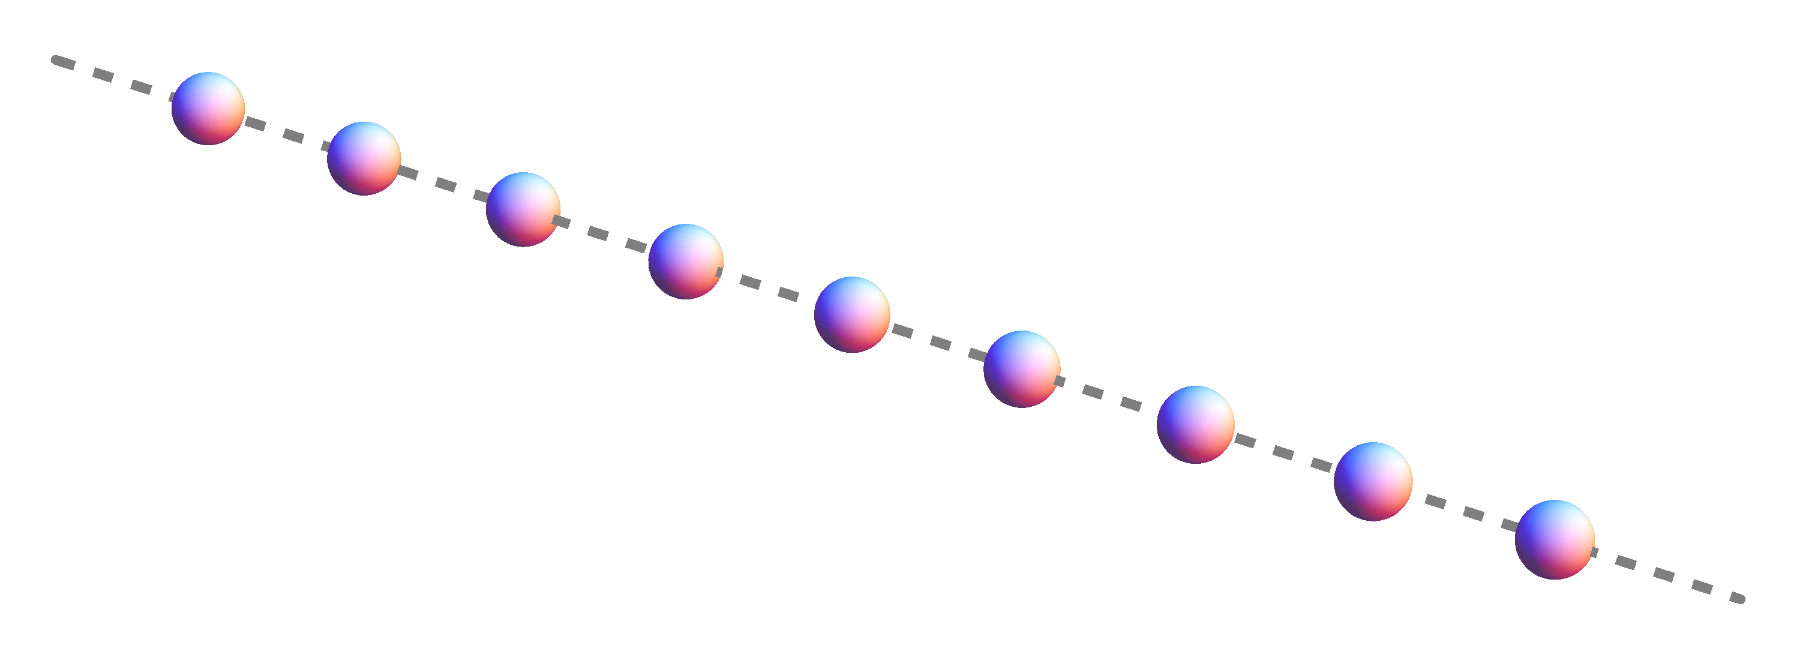
\includegraphics[scale=0.2]{Graphics/TransferMatrix/lattice_1d.png}
\caption{A lattice in one dimension is a set of regularly spaced units.}
\label{fig:1dlattice} 
\end{figure}

The Ising model in one dimension is a classical model for ferromagnetism described by a system of $N$ spins situated regularly on a straight line \figref{1dlattice}.  We denote the value of spin $i$ by $\sigma_i$ which can only take discrete values -1 and 1. In the system we have an external magnetic field interaction of strength $B$, a coupling constant between spin pairs with strength $J$, and the atomic magnetic moment $\mu$. The Hamiltonian for a one-dimensional Ising model is \cite{Newell1953,Yeomans1992}
%
\begin{equation}\label{1disinghamiltonian}
H=-\mu B\sum^{N}_{i=1}\sigma_{i}-J\sum^{N}_{i=1}\sigma_{i}\sigma_{i+1}
\end{equation}
%
where we impose a periodic boundary condition such that 
%
\begin{equation}\label{1disingboundarycondition}
\sigma_{N+1}=\sigma_{1}
\end{equation}
%
This changes the geometry of the straight line lattice into a circle where $\sigma_{N}$ and $\sigma_{1}$ become adjacent neighbours \figref{1dlatticeclosed}. In the Hamiltonian this allows the last term in the sum of interactions to become $\sigma_{N}\sigma_{1}$. Inserting the Hamiltonian into the partition function we get 
%
%The choice of boundary conditions becomes irrelevant in the thermodynamic limit \cite{Yeomans1992}
%
\begin{align}
Z &=\sum\exp\left( -\beta H\right)\\
&=\sum_{\{\sigma_{i}=\pm1\}}\exp\left(\beta\mu B\sum^{N}_{i=1}\sigma_{i}+\beta J\sum^{N}_{i=1}\sigma_{i}\sigma_{i+1}\right)\\
&=\sum_{\{\sigma_{i}=\pm1\}}\prod^{N}_{i=1}\exp\left( \beta \mu B\sigma_{i}\right)\exp\left(\beta J\sigma_{i}\sigma_{i+1}\right) \label{1dising1}
\end{align}
%
\begin{figure}[bp]
\centering 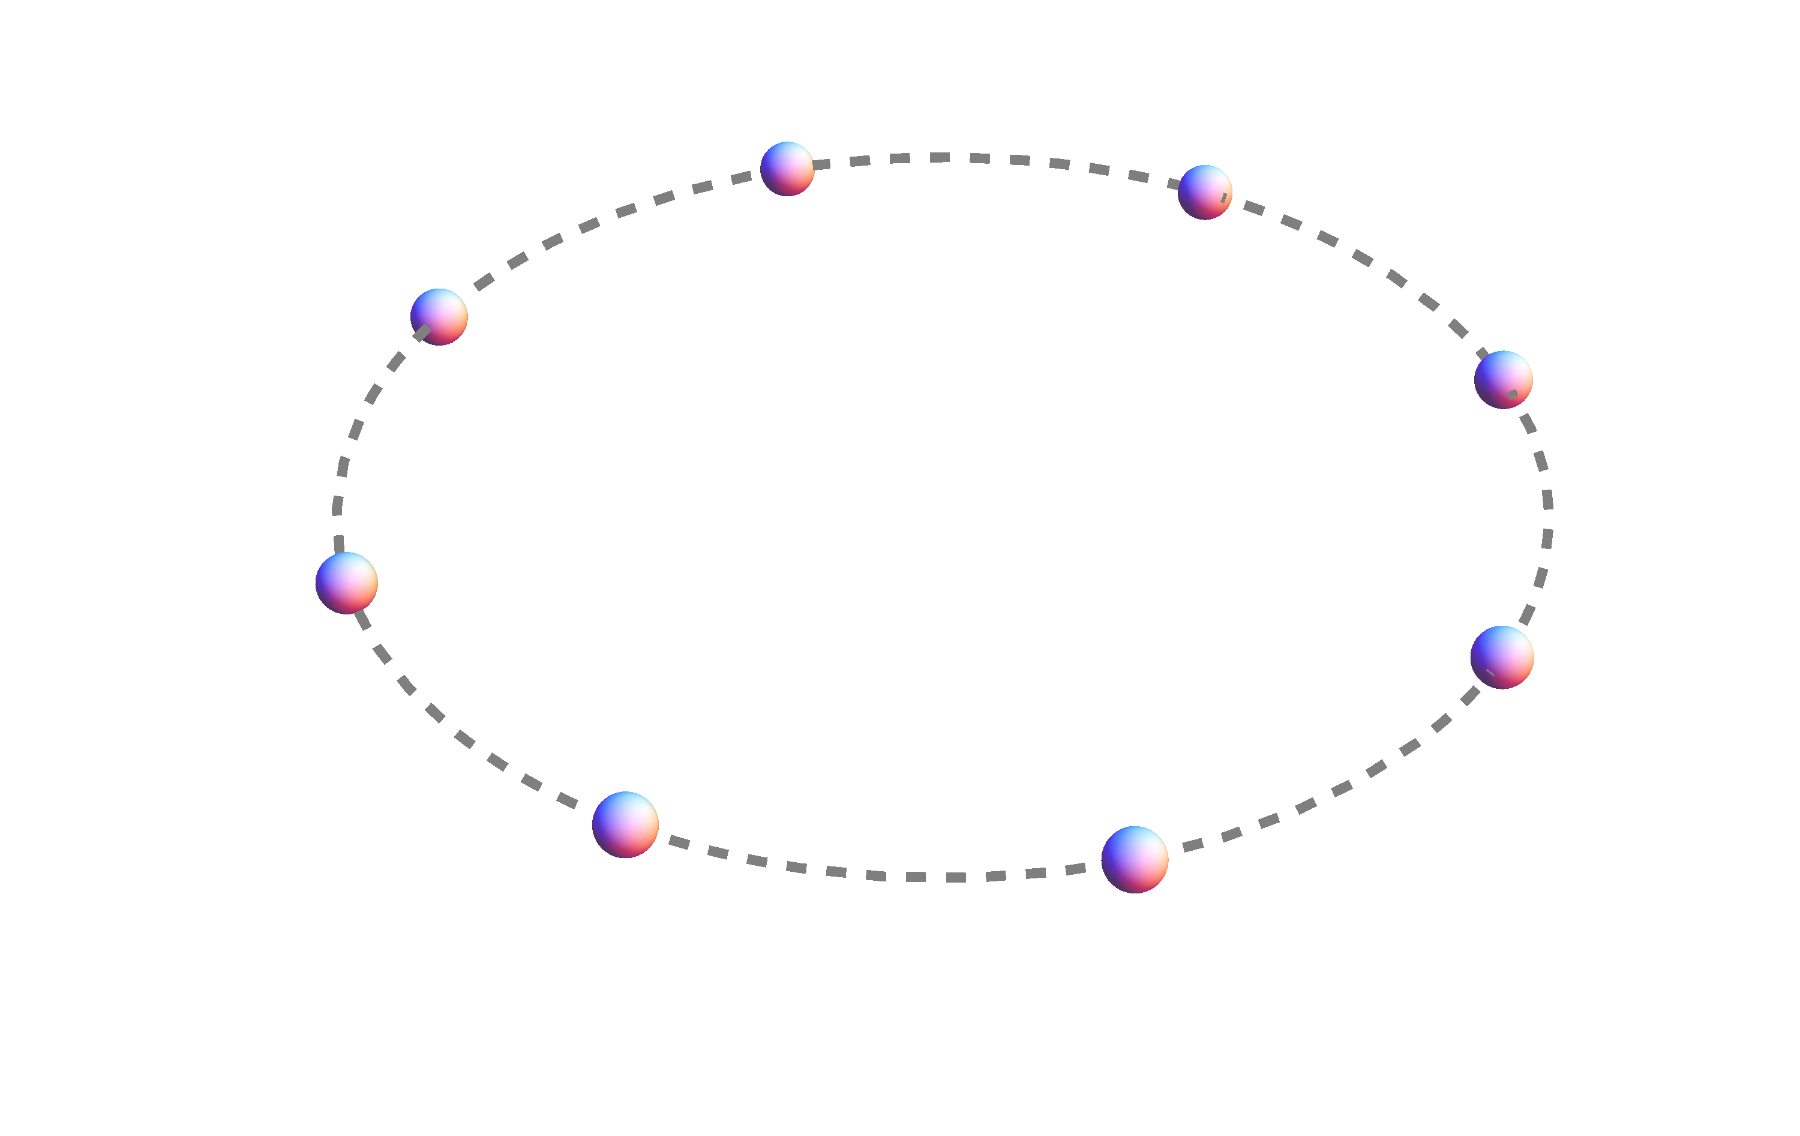
\includegraphics[scale=0.2]{Graphics/TransferMatrix/lattice_1d_closed.png}
\caption{A lattice in one dimension with periodic boundary conditions forms a circle.}
\label{fig:1dlatticeclosed} 
\end{figure}
%
The product of contributions from each spin in the exponential allows us to group adjacent spins together. If we do  this \eqref{1dising1} becomes \cite{Yeomans1992}
%
\begin{align}\label{1disingbeforematrixform}
Z&=\sum_{\{\sigma_{i}=\pm1\}}\exp\left(\beta J\sigma_{1}\sigma_{2}+\frac{\beta B\left(\sigma_{1}+\sigma_{2}\right)}{2}\right)\exp\left(\beta J\sigma_{2}\sigma_{3}+\frac{\beta B\left(\sigma_{2}+\sigma_{3}\right)}{2}\right)...\\
&...\exp\left(\beta J\sigma_{N-1}\sigma_{N}+\frac{\beta B\left(\sigma_{N-1}+\sigma_{N}\right)}{2}\right)\exp\left(\beta J\sigma_{N}\sigma_{1}+\frac{\beta B\left(\sigma_{N}+\sigma_{1}\right)}{2}\right)\nonumber
\end{align}
%
Next we introduce $T\left(\sigma_{i},\sigma_{i+1}\right)$,  which are the elements of a transfer matrix $T$. The rows are labelled by the values of $\sigma_{i}$ and columns by the values $\sigma_{i+1}$.
%
\begin{equation}\label{1disingtransfermatrix}
T\left(\sigma_{i},\sigma_{i+1}\right)=\exp\left(\beta J\sigma_{i}\sigma_{i+1}+\frac{\beta B\left(\sigma_{i}+\sigma_{i+1}\right)}{2}\right)
\end{equation}
%
If we write out the transfer matrix explicitly we get a $2 \times 2$ matrix
%
\begin{equation}
\bordermatrix{&\sigma_{i}=1&\sigma_{i+1}=-1 \cr
\sigma_{i}=1 & \exp\left(\beta J+B\right) & \exp\left(-\beta J \right) \cr
\sigma_{i+1}=-1 & \exp\left(-\beta J \right) & \exp\left(\beta J-B\right) \cr }
\end{equation}
%
Substituting \eqref{1disingtransfermatrix} into \eqref{1disingbeforematrixform}, the transfer matrix allows us to express the partition function  as a product of matrices \cite{Yeomans1992}
%
\begin{equation}
Z=\sum_{\{\sigma_{i}=\pm1\}}T\left(\sigma_{1},\sigma_{2}\right)T\left(\sigma_{2},\sigma_{3}\right)...T\left(\sigma_{N-1},\sigma_{N}\right)T\left(\sigma_{N},\sigma_{1}\right)=\mbox{tr}\left( T^{N}\right)
\end{equation}
%
This equation reduces the calculation of the partition function to the calculation of the trace of an unknown matrix $T^{N}$ . We know from linear algebra that the trace is invariant under cyclic permutations, and therefore using this property in conjunction with an appropriate unitary matrix $U$ and its inverse $U^{-1}$ we can convert the transfer matrix into a diagonal form
%
\begin{equation}
U^{-1}TU= \Lambda =\begin{pmatrix}
\lambda_1 & 0 \\ 
0 & \lambda_2 
\end{pmatrix}
\end{equation}
%
Where $\lambda_1$ and $\lambda_2$ are the eigenvalues of the transfer matrix $T$. Inserting this into the partition function we get
%
\begin{equation}
Z=\mbox{tr}\left(T^{N}\right) = \mbox{tr}\left(\Lambda^{N}\right) = \lambda_1^{N} + \lambda_2^{N}
\end{equation}
%
The eigenvalues of the transfer matrix can be calculated using the eigenvalue equation without explicitly knowing the form of the corresponding eigenvectors
%
\begin{equation}
\det \left| T-\lambda_{i}I\right| =
\begin{vmatrix}
\exp\left(\beta J+\beta B\right)-\lambda_1 & \exp\left(-\beta J \right) \\ \exp\left(-\beta J \right) & \exp\left(\beta J-\beta B\right)-\lambda_2 
\end{vmatrix}=0
\end{equation}
%
where the eigenvalues are \cite{Plischke2006,Yeomans1992}
%
\begin{equation}
\lambda_{1,2}=\exp\left( \beta J \right)\cosh \beta B\pm\sqrt{ \exp\left(2 \beta J\right)\sinh^{2}\beta B + \exp\left(-2\beta J\right)}
\end{equation}
%
The analysis using the transfer matrix gives surprising results in the thermodynamic limit $N \to \infty$ where the boundary effects become negligible only the largest eigenvalue is relevant. In the thermodynamic limit the free energy per spin is given by
%
\begin{align}
F&=-k_{B}T\lim_{N\to\infty}\frac{1}{N}\ln Z_{N}\\
&=-k_{B}T\lim_{N\to\infty}\frac{1}{N}\ln  \left\{ \lambda_{1}^{N}+\lambda_{2}^{N}\right\} \label{fe_2b2}
\end{align}
%
For the more general case where the transfer matrix is larger than a $2 \times 2$ matrix the set of eigenvalues go beyond $\lambda_{1}$ and $\lambda_{2}$, and \eqref{fe_2b2} becomes  
%
\begin{equation}
F=-k_{B}T\lim_{x\to\infty}\frac{1}{N}\ln \left\{ \lambda_{1}^{N}\left(1+\sum_{i}\frac{\lambda_{i}^{N}}{\lambda_{1}^{N}} \right)\right\} \label{fe_general}
\end{equation}
%
With $\lambda_{1}$ being the largest eigenvalue. Since the ratio $\lambda_{i}/\lambda_{1}$ is always less than unity, taking $N\to\infty$ leads to $\left(\lambda_{i}/\lambda_{1}\right)^{N}\to 0$ and hence
%
\begin{equation}
F=-k_{B} T \ln\lambda_{1}
\end{equation}
%
This elegantly shows that thermodynamic quantities in the thermodynamic limit $N\to\infty$ depend only on the largest eigenvalue of the transfer matrix, which is often easier to calculate than the entire spectrum of the matrix. Since this is also true for other interacting many-particle systems treated with the transfer matrix method the problem of finding the exact solution within the transfer-matrix approach is reduced to finding the largest eigenvalue. 

\section{Two-Dimensional Ising Model}

For a two dimensional model we consider a spin-$\frac{1}{2}$ Ising model on a square lattice in a vanishing external field. The lattice is defined by $R$ rows and $C$ columns and the Hamiltonian can be written as \cite{Schultz1964}
%
\begin{equation}
H=-J\left(\sum_{i=1}^{R}\sum_{j=1}^{C}\sigma_{i,j}\sigma_{i+1,j}+\sum_{i=1}^{R}\sum_{j=1}^{C}\sigma_{i,j+1}\sigma_{i,j}\right) 
\end{equation}

\begin{figure}[htp]
\centering 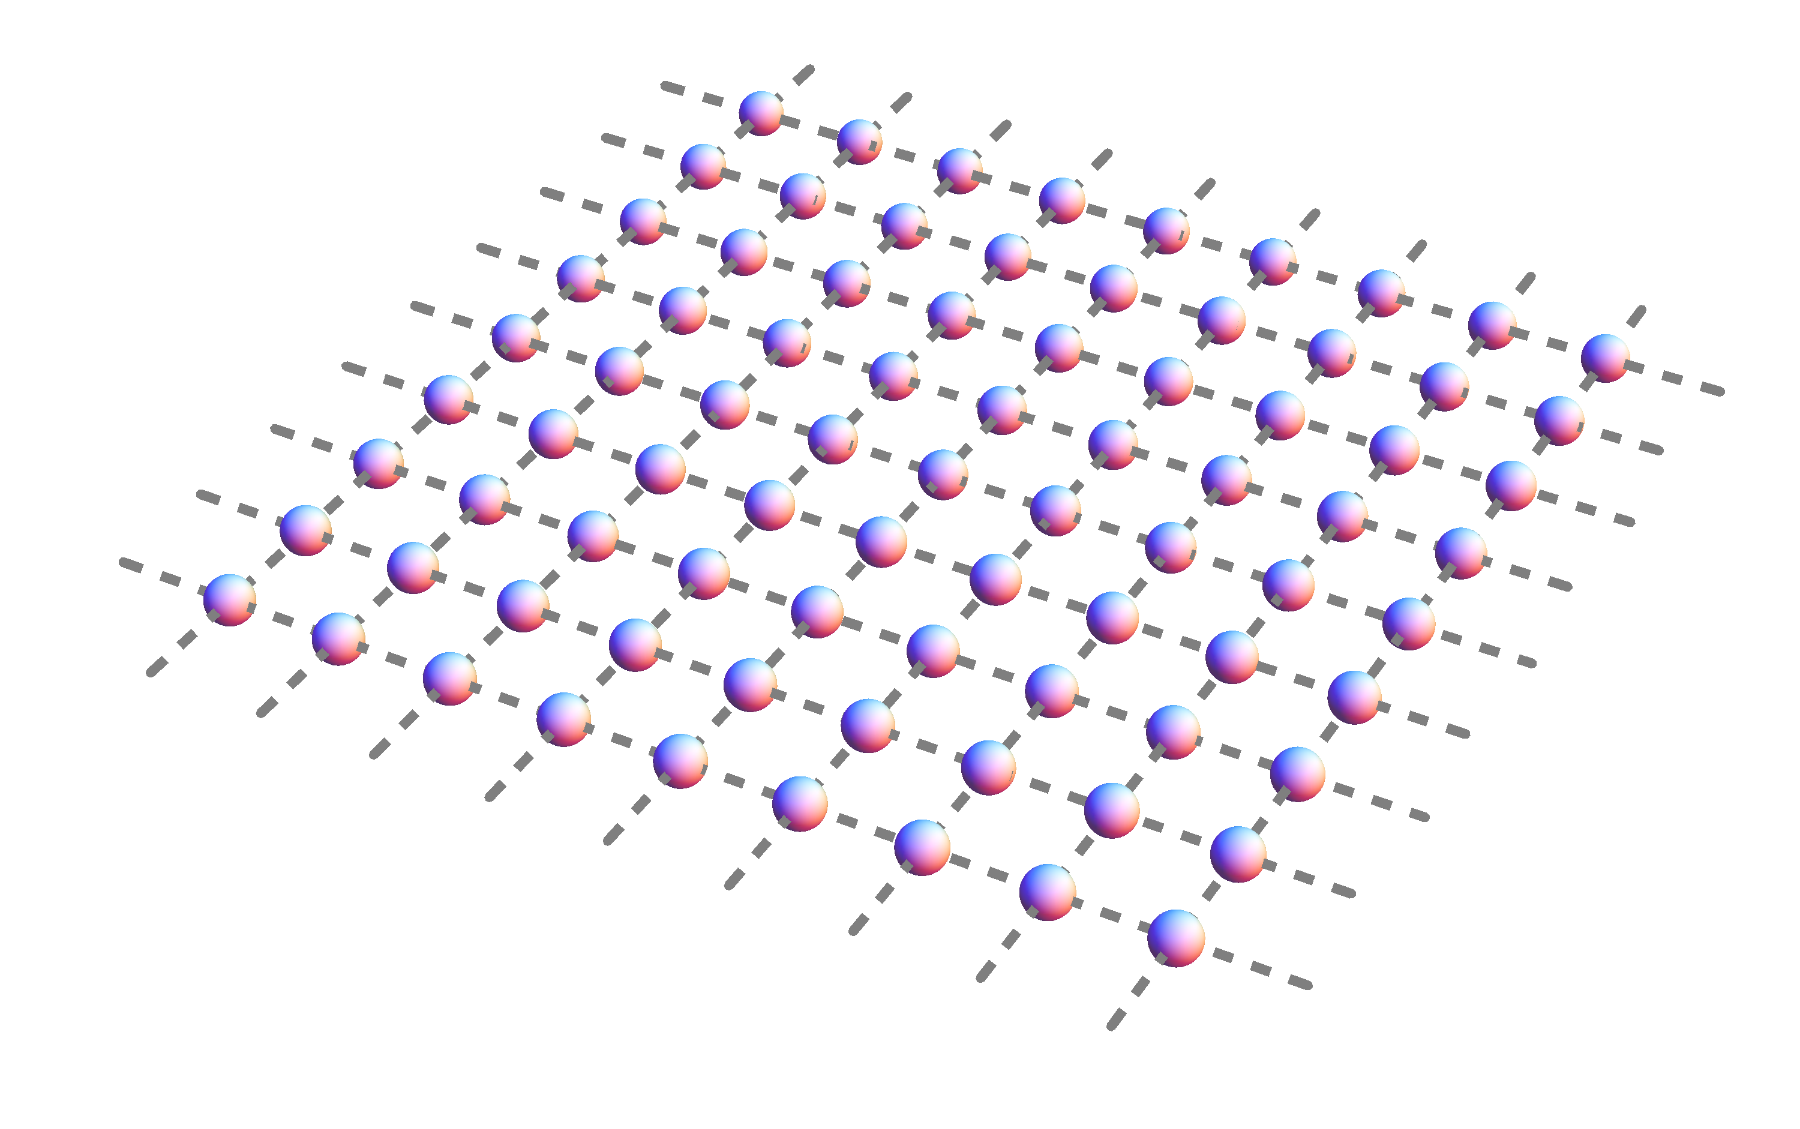
\includegraphics[scale=0.2]{Graphics/TransferMatrix/lattice_2d.png}
\caption{A lattice in two dimensions.}
\label{fig:2dlattice} 
\end{figure}
%
The summations contain two spin coupling interactions between nearest-neighbours: one is for adjacent rows of the square lattice, while the other takes into account adjacent columns. Again, we impose boundary conditions such that the square lattice is continuous
%
\begin{align}
\label{2disingboundarycondition1}
\sigma_{R+1,j}&=\sigma_{1,j}\quad \text{where $j=1,2,3,...,C$}\\
\label{2disingboundarycondition2}
\sigma_{i,C+1}&=\sigma_{i,1}\quad \text{where $i=1,2,3,...,R$}
\end{align}
%
The periodicity of the square lattice makes it topologically equivalent to a 2-torus where the $C^{th}$ column is coupled to the first column, and the  $R^{th}$ row is coupled to the first row. 
%
\begin{figure}[htp]
\centering 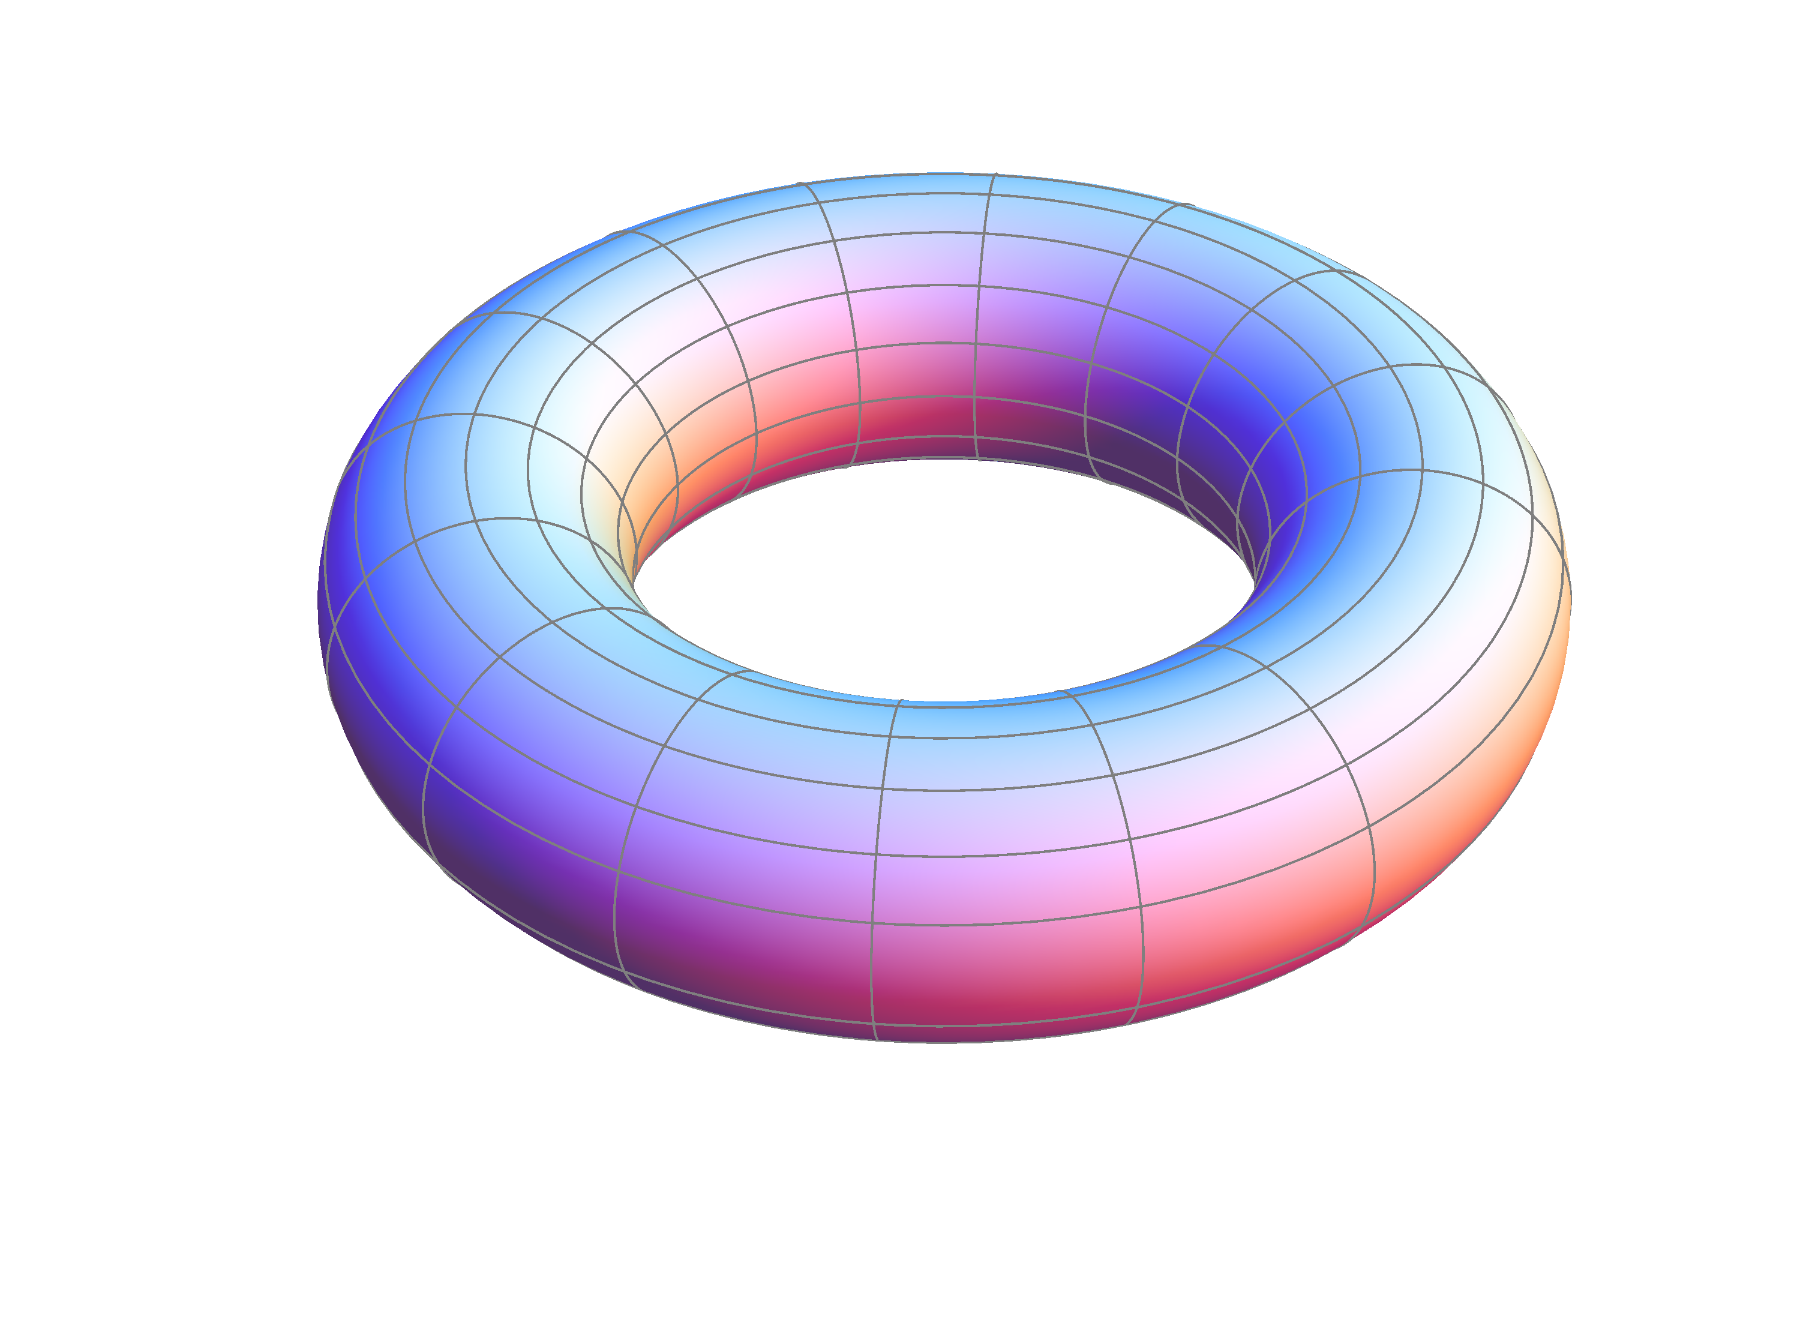
\includegraphics[scale=0.25]{Graphics/TransferMatrix/torus.png}
\caption{The boundary conditions in the vertical and horizontal directions wraps the square lattice into a 2-torus.}
\label{fig:torus} 
\end{figure}
%
We then set the the overall spin configuration of the $j^{th}$ column of spins by a new variable $\xi_{j}$ which has $2^{R}$ possible spin configurations.
%
\begin{equation}
\xi_{j}=\left(\sigma_{1,j},\sigma_{2,j},\sigma_{3,j},\sigma_{4,j},.....,\sigma_{R,j}\right)
\end{equation}
%
The Hamiltonian can then be written as a sum of the interaction energy of individual columns, $H_{1}$, and the interaction energy between adjacent columns, $H_{2}$.
%
\begin{align}
H_{1}\left(\xi_{j}\right)&=-J\sum_{i=1}^{R}\sigma_{i,j}\sigma_{i+1,j}\\
H_{2}\left(\xi_{j},\xi_{j+1}\right)&=-J\sum_{i=1}^{R}\sigma_{i,j}\sigma_{i,j+1}
\end{align}
%
The total Hamiltonian is simply
%
\begin{equation}
H\left(\xi\right)=\sum^{C}_{j=1}H_{1}\left(\xi_{j}\right) + H_{2}\left(\xi_{j},\xi_{j+1} \right)
\end{equation}
%
In the symmetric form the Hamiltonian is
%
\begin{equation}
H\left(\xi\right)= \sum^{C}_{j=1}\frac{1}{2} H_{1} \left(\xi_{j}\right) +\frac{1}{2} H_{1}\left( \xi_{j+1}\right) +  H_{2}\left(\xi_{j},\xi_{j+1} \right)
\end{equation}
%
Inserting this into the partition function  we get the relation
%
\begin{align}
Z&=\sum_{\xi_1}\sum_{\xi_2}\sum_{\xi_3}...\sum_{\xi_C}\exp\left(\sum^{C}_{j=1}-\frac{\beta}{2}\left( H_{1}\left(\xi_{j}\right) +H_{1}\left( \xi_{j+1}\right)\right) -  \beta H_{2}\left(\xi_{j},\xi_{j+1} \right) \right)\nonumber\\
&=\sum_{\xi_1}\sum_{\xi_2}\sum_{\xi_3}...\sum_{\xi_C}\prod_{j=1}^{C}\exp\left( -\frac{\beta}{2}\left( H_{1}\left(\xi_{j}\right) + H_{1}\left(\xi_{j+1}\right)\right) -  \beta H_{2}\left(\xi_{j},\xi_{j+1} \right) \right)
\end{align}
%
which evidently demonstrates the transfer matrix for the 2D Ising model to be
%
\begin{align}
T\left(\xi_j,\xi_{j+1}\right)&= \exp\left( -\frac{\beta}{2}\left( H_{1}\left(\xi_{j}\right) + H_{1}\left(\xi_{j+1}\right)\right) -  \beta H_{2}\left(\xi_{j},\xi_{j+1} \right) \right) \nonumber\\
&=\exp\left( \frac{\beta J}{2}\left( \sum_{i=1}^{R}\sigma_{i,j}\sigma_{i+1,j}   +   \sum_{i=1}^{R}\sigma_{i,j+1}\sigma_{i+1,j+1} \right) + \beta J\sum^{R}_{i=1}\sigma_{i,j}\sigma_{i,j+1} \right)
\end{align}
%
Using these transfer matrices in the partition function we get
%
\begin{equation}
Z=\sum_{\xi_1}\sum_{\xi_2}...\sum_{\xi_C}T\left(\xi_1,\xi_2\right)T\left(\xi_2,\xi_3\right)...T\left(\xi_{C-1},\xi_C\right)T\left(\xi_C,\xi_{1}\right) \label{tm_torus}
\end{equation}
%
At this point we introduce a Kronecker delta defined by the boundary conditions $\delta_{\xi_{C+1},\xi_{1} }$ and then apply the completeness relation to express the delta function as set of eigenfunctions, $\psi_{\mu}$, of the transfer matrix $T\left(\xi_i,\xi_{i+1}\right)$.
%
\begin{equation}
\delta_{\xi_{C+1},\xi_{1} }=\sum_{\mu}\psi_{\mu}^{*}\left(\xi_{1} \right)\psi_{\mu}\left(\xi_{C+1}\right)
\end{equation}
%
The eigenvalue equation is
%
\begin{equation}\label{2devalequation}
\sum_{\xi_{i}}T\left(\xi_i,\xi_{i+1}\right)\psi_{\mu}\left(\xi_{i}\right) = \lambda_{\mu}\psi_{\mu}\left(\xi_{i+1}\right)
\end{equation}
%
The partition function with the complete set of eigenfunctions becomes
%
\begin{equation}
Z=\sum_{\mu}\sum_{\xi_1}\sum_{\xi_2}...\sum_{\xi_C}\sum_{\xi_{C+1}}\psi_{\mu}^{*}\left(\xi_{1} \right)T\left(\xi_1,\xi_2\right)T\left(\xi_2,\xi_3\right)...T\left(\xi_{C-1},\xi_C\right)T\left(\xi_C,\xi_{C+1}\right)\psi_{\mu}\left(\xi_{C+1}\right)\\
\end{equation}
%
Now we use equation \eqref{2devalequation} to contract each transfer matrix in the sum with an appropriate eigenfunction, leaving behind an eigenvalue which is a scalar quantity. We get
%
\begin{equation}
Z=\mbox{tr}\left(T^{C}\right)=\sum_{j=1}^{2^{R}} \lambda_{j}^{C}
\end{equation}
%
In the thermodynamic limit the free energy per spring for a 2D Ising model becomes
%
\begin{align}
F&=-k_{B}T\lim_{R\to\infty}\lim_{C\to\infty}\left\{\frac{1}{RC}\ln \left(\lambda^{C}_{1} + \lambda^{C}_{2} + ... + \lambda^{C}_{2^{R}}\right)\right\} \\
&= -k_{B}T\lim_{R\to\infty}\frac{1}{R}\ln\lambda_{1} - k_{B}T\lim_{R\to\infty}\lim_{C\to\infty}\frac{1}{RC}\ln\left[1+\sum_{i}^{2^R}\left(\frac{\lambda_{g}}{\lambda_{1}}\right)^{C}\right]\\
&= -k_{B}T\lim_{R\to\infty}\frac{1}{R} \ln \lambda_{1}
\end{align}
%
The calculation of the largest eigenvalue of the $T\left(\xi_i,\xi_{i+1}\right)$ matrix goes beyond the scope of this thesis but here again we have clearly demonstrated the use of the transfer matrix method in finding the exact solution to the 2D Ising model.
%
\begin{figure}[bp]
\centering 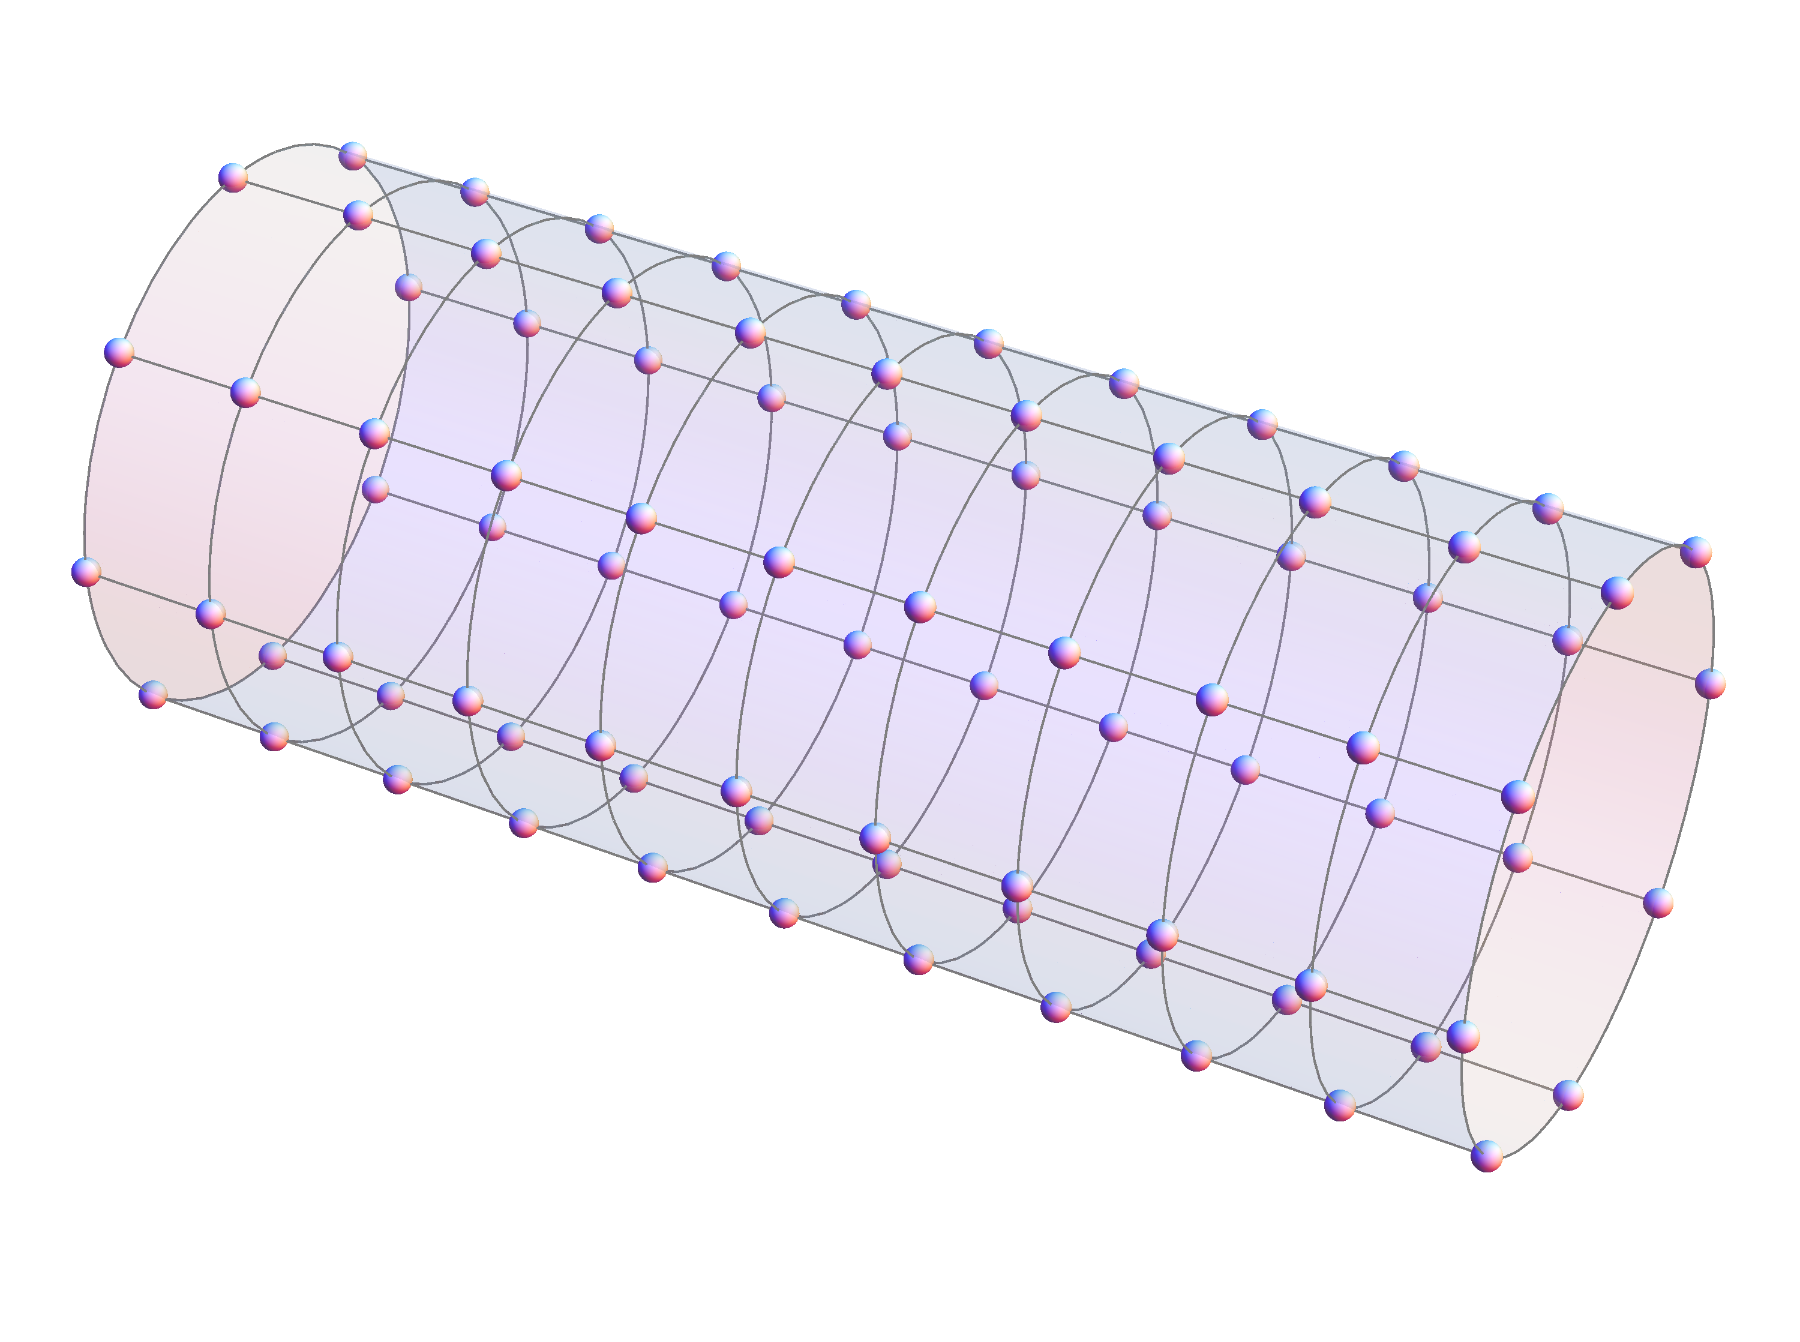
\includegraphics[scale=0.2]{Graphics/TransferMatrix/lattice_cylinder.png}
\caption{A single boundary condition in the vertical direction wraps the square lattice into a cylinder.}
\label{fig:cylinder} 
\end{figure}
%
Expanding on the two dimensional model we can consider the lattice subject to just one boundary condition, \eqref{2disingboundarycondition2}, and find an expression for the partition function when the topology of the lattice is folded into a cylinder.  We continue from \eqref{tm_torus}, but omit the final transfer matrix $T\left(\xi_C,\xi_1\right)$. The partition function becomes
%
\begin{align}
\label{tm_cylinder}
Z=\sum_{\xi_1}\sum_{\xi_2}...\sum_{\xi_C}&T\left(\xi_1,\xi_2\right)T\left(\xi_2,\xi_3\right)T\left(\xi_3,\xi_4\right)...T\left(\xi_{C-1},\xi_C\right)\\
&\times\exp\left(-\frac{\beta H\left( \xi_1\right)}{2}\right)\exp\left(-\frac{\beta H\left( \xi_C\right)}{2}\right)
\end{align}
%
Here we introduce a Kronecker delta function with a dummy variable $\xi_\alpha$ such that
%
\begin{equation}\label{bc_cylin}
\delta_{\xi_1,\xi_\alpha}=\sum_{\mu}\psi_{\mu}^{*}\left(\xi_{1} \right)\psi_{\mu}\left(\xi_{\alpha}\right)
\end{equation}
%
Inserting this into \eqref{tm_cylinder} 

%
\begin{align}
Z\left(\xi_{\alpha}\right)=\sum_{\mu}\sum_{\xi_1}\sum_{\xi_2}...\sum_{\xi_C}&\psi_{\mu}^{*}\left(\xi_{1} \right)T\left(\xi_1,\xi_2\right)T\left(\xi_2,\xi_3\right)T\left(\xi_3,\xi_4\right)...T\left(\xi_{C-1},\xi_C\right)\psi_{\mu}\left(\xi_{\alpha}\right)\\
&\times\exp\left(-\frac{\beta H\left( \xi_1\right)}{2}\right)\exp\left(-\frac{\beta H\left( \xi_C\right)}{2}\right)\nonumber
\end{align}
%
We then proceed to contract each transfer matrix in the sum from $\xi_1$ to get an expression for the partition function
%
\begin{equation}
Z\left(\xi_{\alpha}\right)=\sum_{\mu}\sum_{\xi_C}\lambda_{\mu}^{C-1}\psi_{\mu}^{*}\left(\xi_{C} \right)\psi_{\mu}\left(\xi_{\alpha}\right)\exp\left(-\frac{\beta H\left( \xi_{\alpha}\right)}{2}\right)\exp\left(-\frac{\beta H\left( \xi_C\right)}{2}\right)
\end{equation}



%\chapter{Polymers}

Studying how life on earth first originated from inert matter the Miller-Urey experiment simulated hypothetical conditions thought to be present at the time on earth over 4 billion years ago \cite{Miller1959}. Under certain conditions elements like hydrogen, carbon, oxygen and nitrogen synthesized simple organic compounds which in turn reacted to form larger structures of greater complexity. It was found that the organic compounds formed in the experiment were the same compounds that are able to go on further, and assemble more complex biomolecules such as DNA, proteins, and other biopolymers. These formed some of the earliest natural polymers in the world today. Some of these natural polymers include, nucleic acids and proteins which carry and manipulate biological information whereas polysaccharides, a polymer made of glucose as the monomeric unit, provides fuel for cell activity and serves as the structural element to living systems \cite{karp2005}. Other examples of natural polymers include starch, ligin, cellulose, collagen, silk, natural rubber, linen, and a rather more complicated example, wood \cite{Staudinger1953}.  

The discovery of synthetic polymers came in the early nineteenth century but it wouldn't be until the late 1930's that the manufacturing and use of such materials became important. Wartime demands and shortages during World War II encouraged scientists to create replacements for natural materials which were in short supply or unavailable. In this period the use of nylon, acrylic, neoprene, polyethylene, and many more polymers took the place of natural materials that were temporarily unavailable. Since then, the polymer industry has evolved into one of the fastest growing industries in the world. As research in polymeric materials continued the development of synthetic polymers accelerated to play an essential and ubiquitous role in everyday life.

Today polymers still continue to make a profound impact on industry, manufacturing, and technology.  In the field of nanotechnology, polymers are used in nano-electronics where the critical dimension scale for modern devices is now below 100 nm. Other areas include polymer-based biomaterials, nano-particle drug delivery, polymer blends and nano-composites. Nanotechnology is not new to polymer science as prior studies before the nanotechnology revolution involved nano-scale dimensions \cite{Samad2009,Paul2008}.  

\section{Polymer Architecture}

A polymer is a molecule made up by the repetition of a simpler chemical unit called a monomer \cite{bower2002}. They form to become large-chain molecules of very high molecular weight so the term "macromolecule" is often used as a synonym for polymers. If the chain molecule is made up of one type of monomer then the polymer is called a homo-polymer. If there is more than one type of monomer then it is called a copolymer \cite{Pure1996}. 

Polymers can exist in different types of chain configurations which can be either linear, branched or cross-linked. A linear polymer is a polymer molecule in which the atoms are arranged in a long chain like structure. This chain is often called the backbone. Polyethylene is a prime example of a linear polymer which is made up of ethylene monomers joined together to form the polymer. The number of monomer units in polyethylene, $n$, is usually of order of $10^{4}$, but can range between $10^{3}-10^{6}$. In some linear polymers the atoms in the chain will have small chains of atoms attached to them, much smaller than backbone. These small chains are called pendant groups which only have a few atoms. An example of a linear polymer with a pendant group is polyproylene, with it's chemical repeating unit made up of two carbon atoms, with one atom attached to two hydrogen atoms and the other carbon attached to one hydrogen, and one pendent methyl group.

\begin{figure}[htp]
\centering \includegraphics[scale=0.1]{Graphics/polyethylene-repeat-2D.png}
\caption{The stereochemistry of the ethylene monomer that makes polyethylene.}
\label{fig:polyethylene2D}
\end{figure}

\begin{figure}[htp]
\centering \includegraphics[scale=0.3]{Graphics/Polyethylene3D.png}
\caption{A 3D illustration of a polyethylene polymer.}
\label{fig:Polyethylene3D}
\end{figure}

\begin{figure}[htp]
\centering \includegraphics[scale=0.3]{Graphics/Polypropylene3D.png}
\caption{A 3D illustration of a polypropylene polymer.}
\label{fig:Polypropylene3D}
\end{figure}

A linear polymer chain may also contain some side growth that takes place from the main chain so while most of the monomeric units are linked with two others on either side, some monomeric units are linked with a third monomeric unit to form a structure that is called a branched polymer chain. These types of polymers are overwhelmingly linear but with branches attached at random points. Branched polymer molecules cannot pack together as closely as linear molecules so the intermolecular forces holding these polymers together tend to be much weaker.

Branched polymers can further change the architecture of a polymer by allowing the neighbouring polymer strands to interact. This causes the polymer strands to form chemical bonds with other other polymer strands creating a cross-linked network of chain segments in three dimensions. 

\subsection{Chemical and Geometrical Structure}

The chemical structure of polymers depends on the chemical nature of its monomeric units while the geometrical structure depends on the spatial arrangements of the adjacent monomeric units. It is quite possible to have a polymer made up of one type of monomer unit, but to have different geometrical structures. In discussing the spatial arrangement of monomeric units in a polymer chain we often talk of two important terminologies, specifically its configuration and conformation.

\section{Polymer Configuration and Conformation}
%\subsection{Polymer Configuration}

The configuration of the polymer is the arrangement fixed by chemical bonding between the adjacent monomeric units and between the atoms of the individual monomeric units. As long the chemical bonds are not broken or re-formed the configuration of the polymer remains the same. A polymer cannot shift from one configuration to another without breaking or re-forming the chemical bonds \cite{poly_sci_eng,bower2002}.  

%\subsection{Polymer Conformations}

The conformation describes the spatial arrangements of the various atoms and atomic groups in the molecule that may arise from  rotation around single bonds. In macromolecular science such conformations are called micro-conformations or local conformations since they only consist of small molecules controlled by intermolecular forces \cite{Flory1980,Elias1997}. The macro-conformation is the overall shape of the polymer molecule determined by the sum of all the micro-conformations taken by each of the repeating monomeric units.  

An interpretation of the relationships between structure and properties requires comprehensive investigation into the spatial arrangement of the atoms that make the chain molecule and its pendent groups. This essential first stage probes the connection between molecular structure and properties, not being limited to only polymers but also low molecular substances as well. Structural parameters consisting of bond lengths and bond angles may suffice to specify the geometric configuration of a molecule, but for chain molecules, especially in polymers, torsional rotations about skeletal bonds must be taken into account. The spatial configuration of a polymer depends on these angles determining its macro-conformation \cite{Flory1980}.  

At the molecular scale the configuration of a chain molecule in three dimensional space is determined by the length of the bonds $l$ in the chain backbone, by the angle specifying the difference between the directions of successive bonds $\theta$, and by the angle of rotation around the bonds $\phi$. The bond lengths $l$ and bond angles $\theta$ are fixed within narrow limits and so we can treat these quantities as pre-determined geometrical parameters. The spatial configuration of the polymer chain can therefore be determined by the fixed set of parameters $\{l,\theta\}$ and by a variable set of rotational angles $\phi_{1}...\phi_{2}...\phi_{n-2}$ about each of the $n-2$ internal bonds, $n$ being the total number of skeletal bonds in the chain.

Rotations around the single bonds $\{\phi\}$ do not occur freely, but are restricted by a rotational energy barrier determined by the bond itself and by hindrances imposed by steric interactions between local atoms and molecular groups \cite{Plischke2006}. The potentials affecting the torsional rotation of the chain's backbone also has several minima separated by barriers at least several times the thermal energy $kT$ \cite{Flory1980}. The carbon-carbon bond energy as a function of rotational angle for polyethylene is plotted in \figref{pe_potential_ethane}. 

\begin{figure}[htp]
\centering \includegraphics[scale=0.3]{Graphics/pe_potential.png}
\caption{The potential as a function of rotational angle $\phi$ around the $C-C$ bond in the backbone of polyethylene \cite{Hiemenz1984}.}
\label{fig:pe_potential_ethane}
\end{figure}

The bond-orientation at the absolute minimum of this energy where $\phi=0$, is referred to as the trans-configuration. Geometrically it is where all the three single carbon bonds $C_{n-2}-C_{n-1}-C_{n}-C_{n+1}$ lie in a plane arranged such that the carbon atoms are staggered (\figref{Polyethylene3D}). The other configuration at $\phi= \pm{2\pi/3}$ is called gauche-configurations representing a geometric shape where the bonds $C_{n-2}-C_{n-1}$ eclipse $C_{n}-C_{n+1}$. 

The rotational potential energies in polyethylene gives us two limiting cases when looking at thermal energies $RT$. In the first case where $RT$ is greater than $~16kJ/mol$ the $C-C$ bonds overcome all potential barriers allowing all the bonds in the polymer to rotate freely. Where $RT$ is less than $~4kJ/mol$ (gauche-state) the bonds occupy the lowest energy state in the trans-configuration and only move about the equilibrium position. However, the energy difference between the $trans$ and $gauche$ states give thermal energies approximately to, $RT = 2.48 kJ/mol$ at $25^{\circ}C$, which implies that at room temperature the $C-C$ bonds will be interchanging between configurations.

Polymers typically have a very large number of single bonds around which various conformations are possible, and a polymer can therefore have a very large number of conformational states. For a typical polyethylene macromolecule with an $n$ number of $C$ atoms ranging from 1000 to 100,000, the number of molecular conformations becomes extremely large, increasing as an exponential function of $n$. The number of conformational states can potentially be reduced by the steric hindrance and overlapping of the chain itself, but nevertheless, since $n$ is so large reasonably precise statements can be made about the relative probability of particular conformations of a polymer chain using statistical methods \cite{bower2002}.

\chapter{Biopolymers DNA and Collagen}

Macromolecules formed by biochemical reactions are called biopolymers, and like ordinary polymers, they are made up of repeating chemical units called monomers. Homologous biopolymers such as proteins are made up of one type of monomer unit whereas heterologous biopolymers are made up of more than one class of monomeric unit. In contrast to many synthetic polymers the fundamental characteristic of biopolymers is their hierarchical structure. At the atomic level the primary structure of biopolymers specifies the sequence of its monomeric subunits. The build up of monomeric units then forms a secondary structure which describes the macro-conformation the biopolymer takes in three dimensional space. Another feature that characterises polymers is the architecture which can also be linear, branched or even cross-linked.

\section{Deoxyribonucleic Acid (DNA)}

DNA is a biomolecule within cells of living organisms that contain genetic information essential for biological functions. In the the early 1950's X-ray diffraction patterns first gave an insight into the double helical structure of DNA \cite{Watson1953,Kittel1968}. Further research in the later years would provide detailed views of DNA as well as refining ideas about the DNA structure and the interactions with other proteins \cite{Klug2004}. It still continues to be an area of active research for both physical and life sciences.

Today advances in technology enable us to observe and manipulate these molecules in a controlled environment using force spectroscopy techniques; the most common methods include using optical tweezers \cite{Wang1997,VanMameren2009}, magnetic tweezers and atomic force microscopy (AFM) \cite{Marko2003,Lavery2002,Strick2003}. The well publicised structure of the molecule is only a static picture and it is now understood that the dynamics of biological molecules are also essential for their function. Molecular dynamics simulation has shown that chemical reactions that seem to be impossible according to the static molecular structure might indeed take place due to temporary large molecular distortions \cite{Karplus1990,Harris2005}. An example of when this might occur in DNA is when it needs to replicate itself, or when DNA goes through the transcription process with the help of enzymes through biochemical reactions \cite{Marko2003,Dauxois1993}. Here DNA can either be bent, twisted, stretched, compressed, sheared or even locally destroyed requiring a significant amount of energy. Experiments  have measured some of these bulk properties where the twist modulus of DNA was found to be 440 pN $\text{nm}^{2}$ \cite{Bryant2003}, and the stretch modulus was measured to be 1000 pN \cite{Lavery2002,Bustamante2000}.

%However, purely mechanical studies of molecular motion , at constant energy are not sufficient because thermal fluctuations due to environmental interactions play a major role in DNA functioning \cite{Peyrard2004}. Statistical mechanics is a key tool in analysing this behaviour.

\subsection{DNA Structure}  

Made out deoxyribonucleotide monomers, DNA is a biopolymer that belongs to a group of macromolecules called nucleic acids. The composition of each nucleotide consists of three components: the sugar deoxyribose, the heterocyclic (5-carbonic) base that binds to the 1' carbon of the sugar, and the phosphate group that binds to the 5' carbon of the sugar. The polymerisation of these nucleotides form the two backbone strands of DNA where the phosphate group bonds with the 3' carbon of another nucleotide by a 3',5' phosphate-diester covalent bond. Together they form a regular polynucleotide chain with an alternating sugar and phosphate group that is characterised by its polarity from its 5'-end to its 3'-end \cite{Berg2010,Watson2003}. 

In DNA the two strands are of equal length and are aligned anti-parallel to each other coiling round an axis to form a right-handed helix. In this arrangement the negatively charged sugar-phosphate backbones are positioned on the exterior of the double helix structure with the nucleotide bases on the inside being exposed through the major and minor grooves of the double helix structure \figref{dna_space_filled}. 
%
\begin{figure}[t]
\centering
\subfloat[]{\label{fig:dna_structure}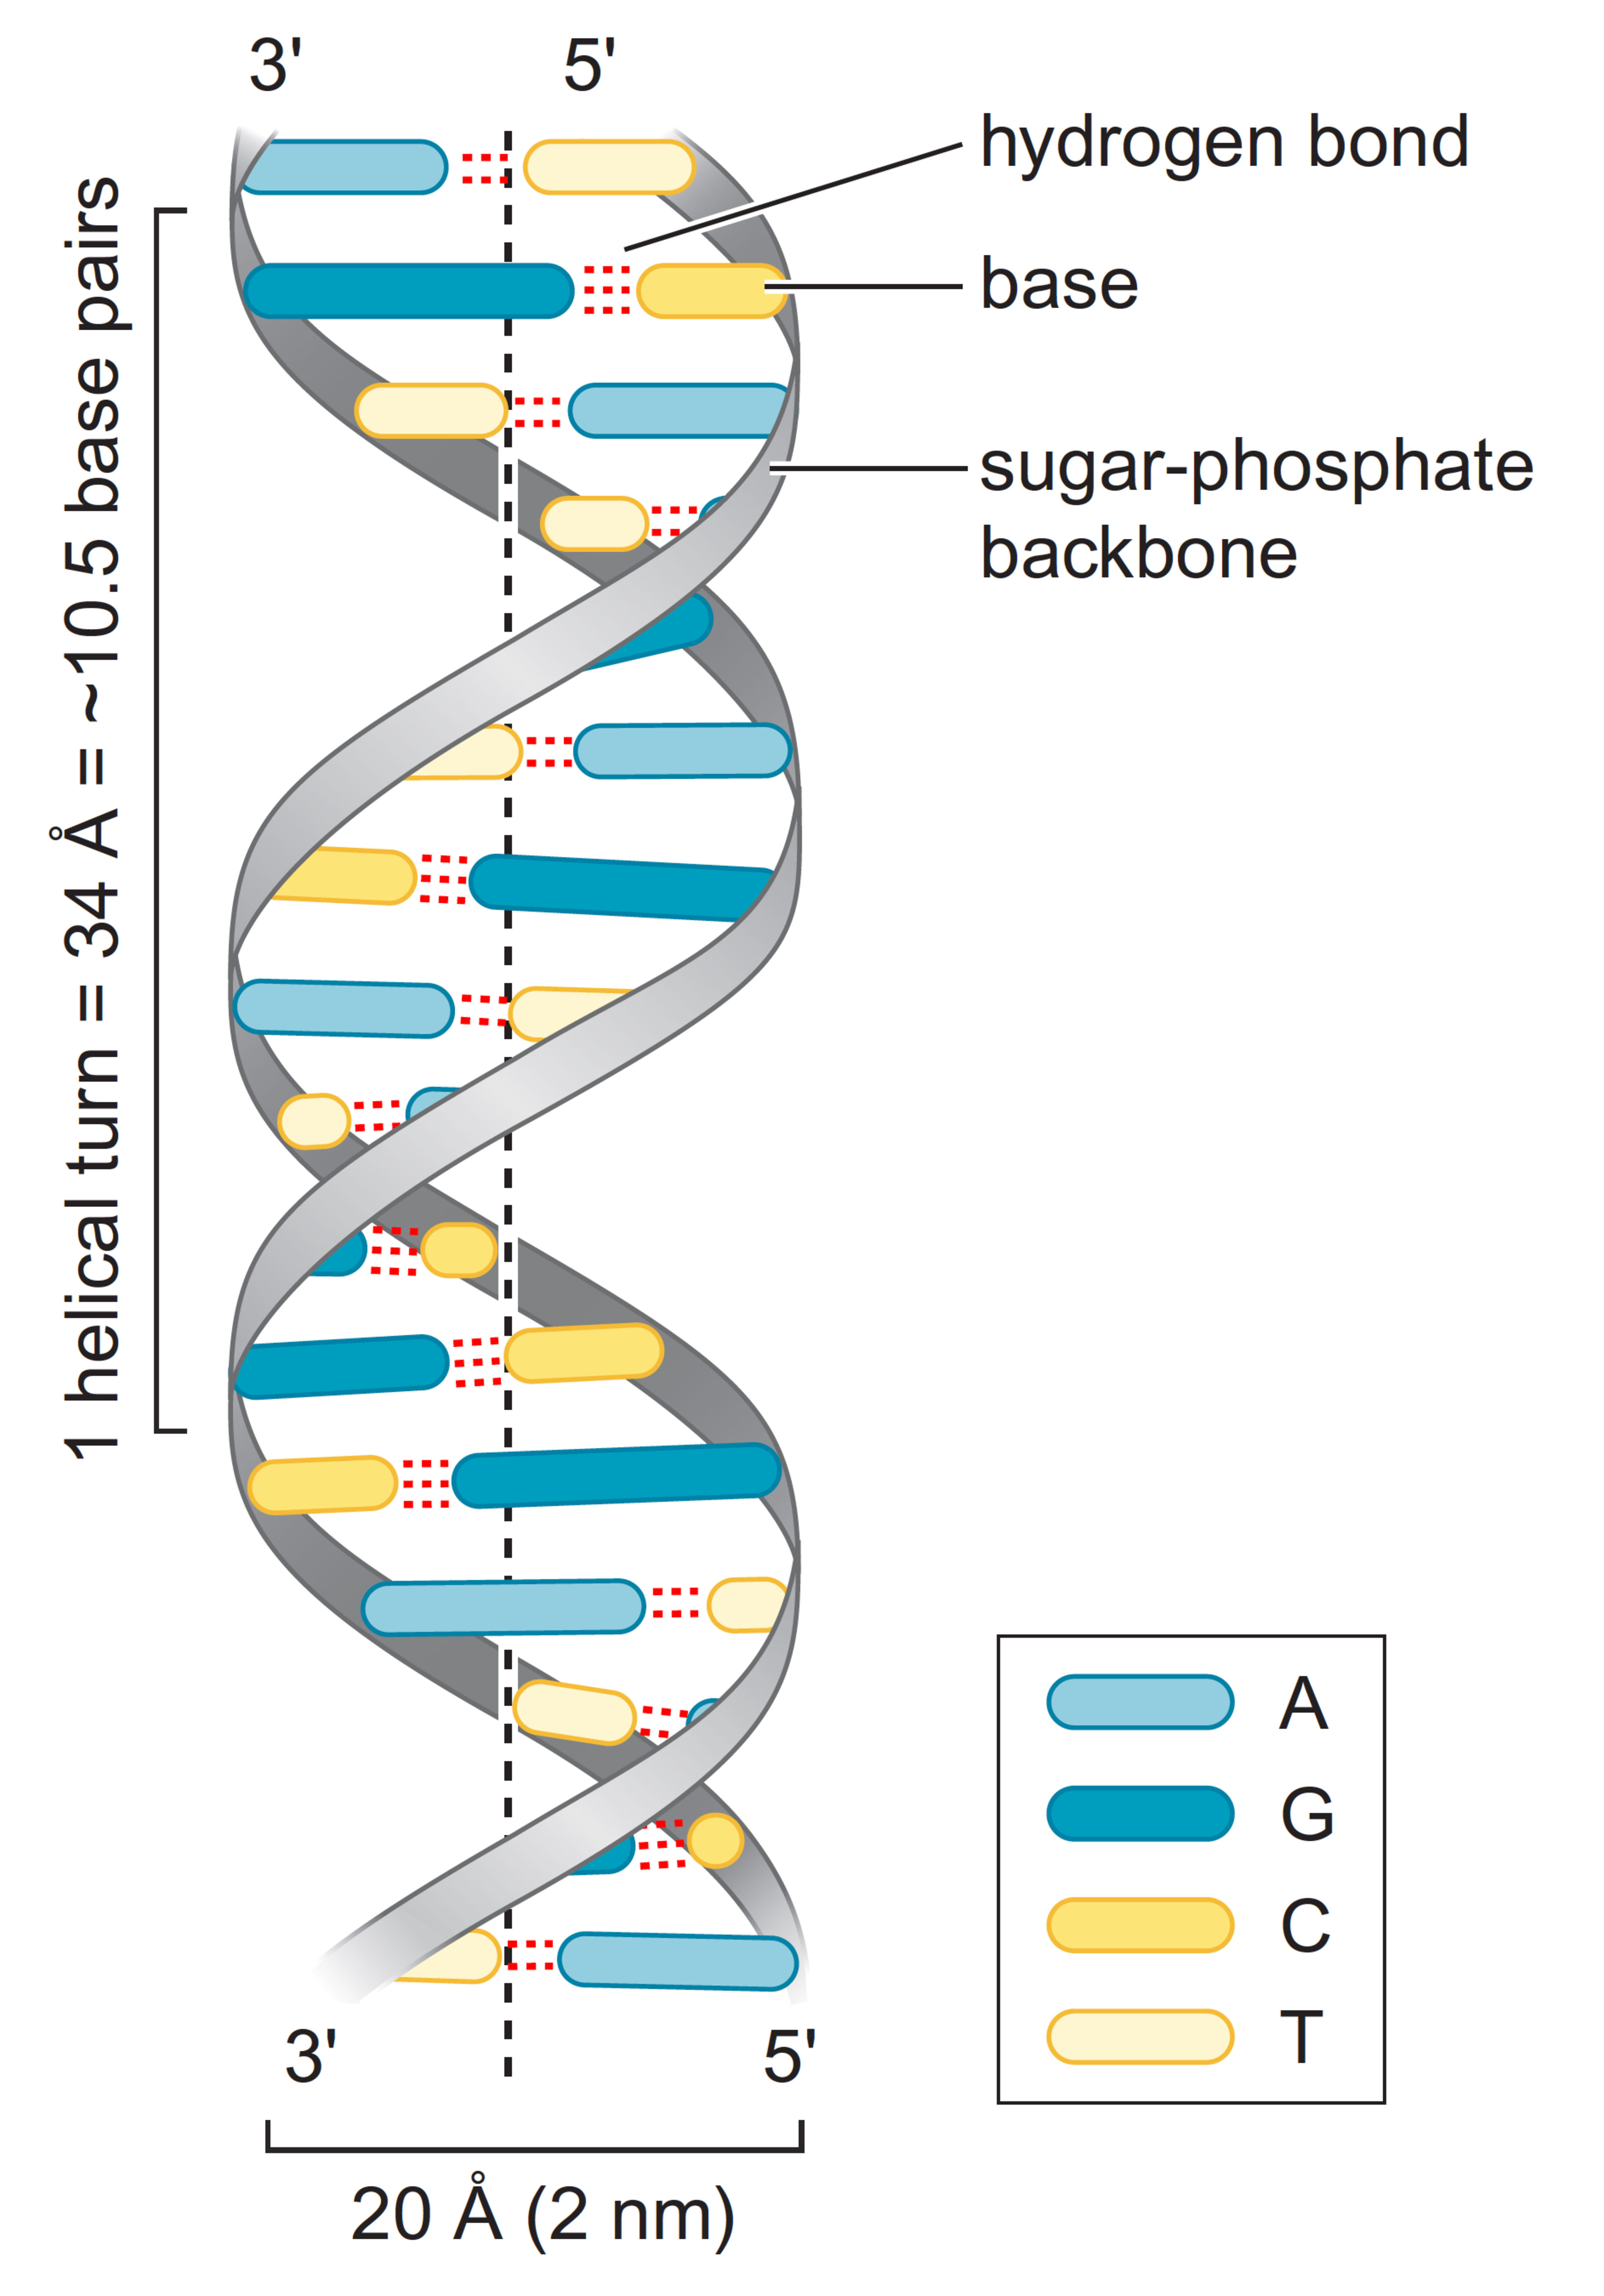
\includegraphics[width=0.4\textwidth]{Graphics/DNA/dna_structure.pdf}}                
\hspace{10mm}
\subfloat[]{\label{fig:dna_space_filled}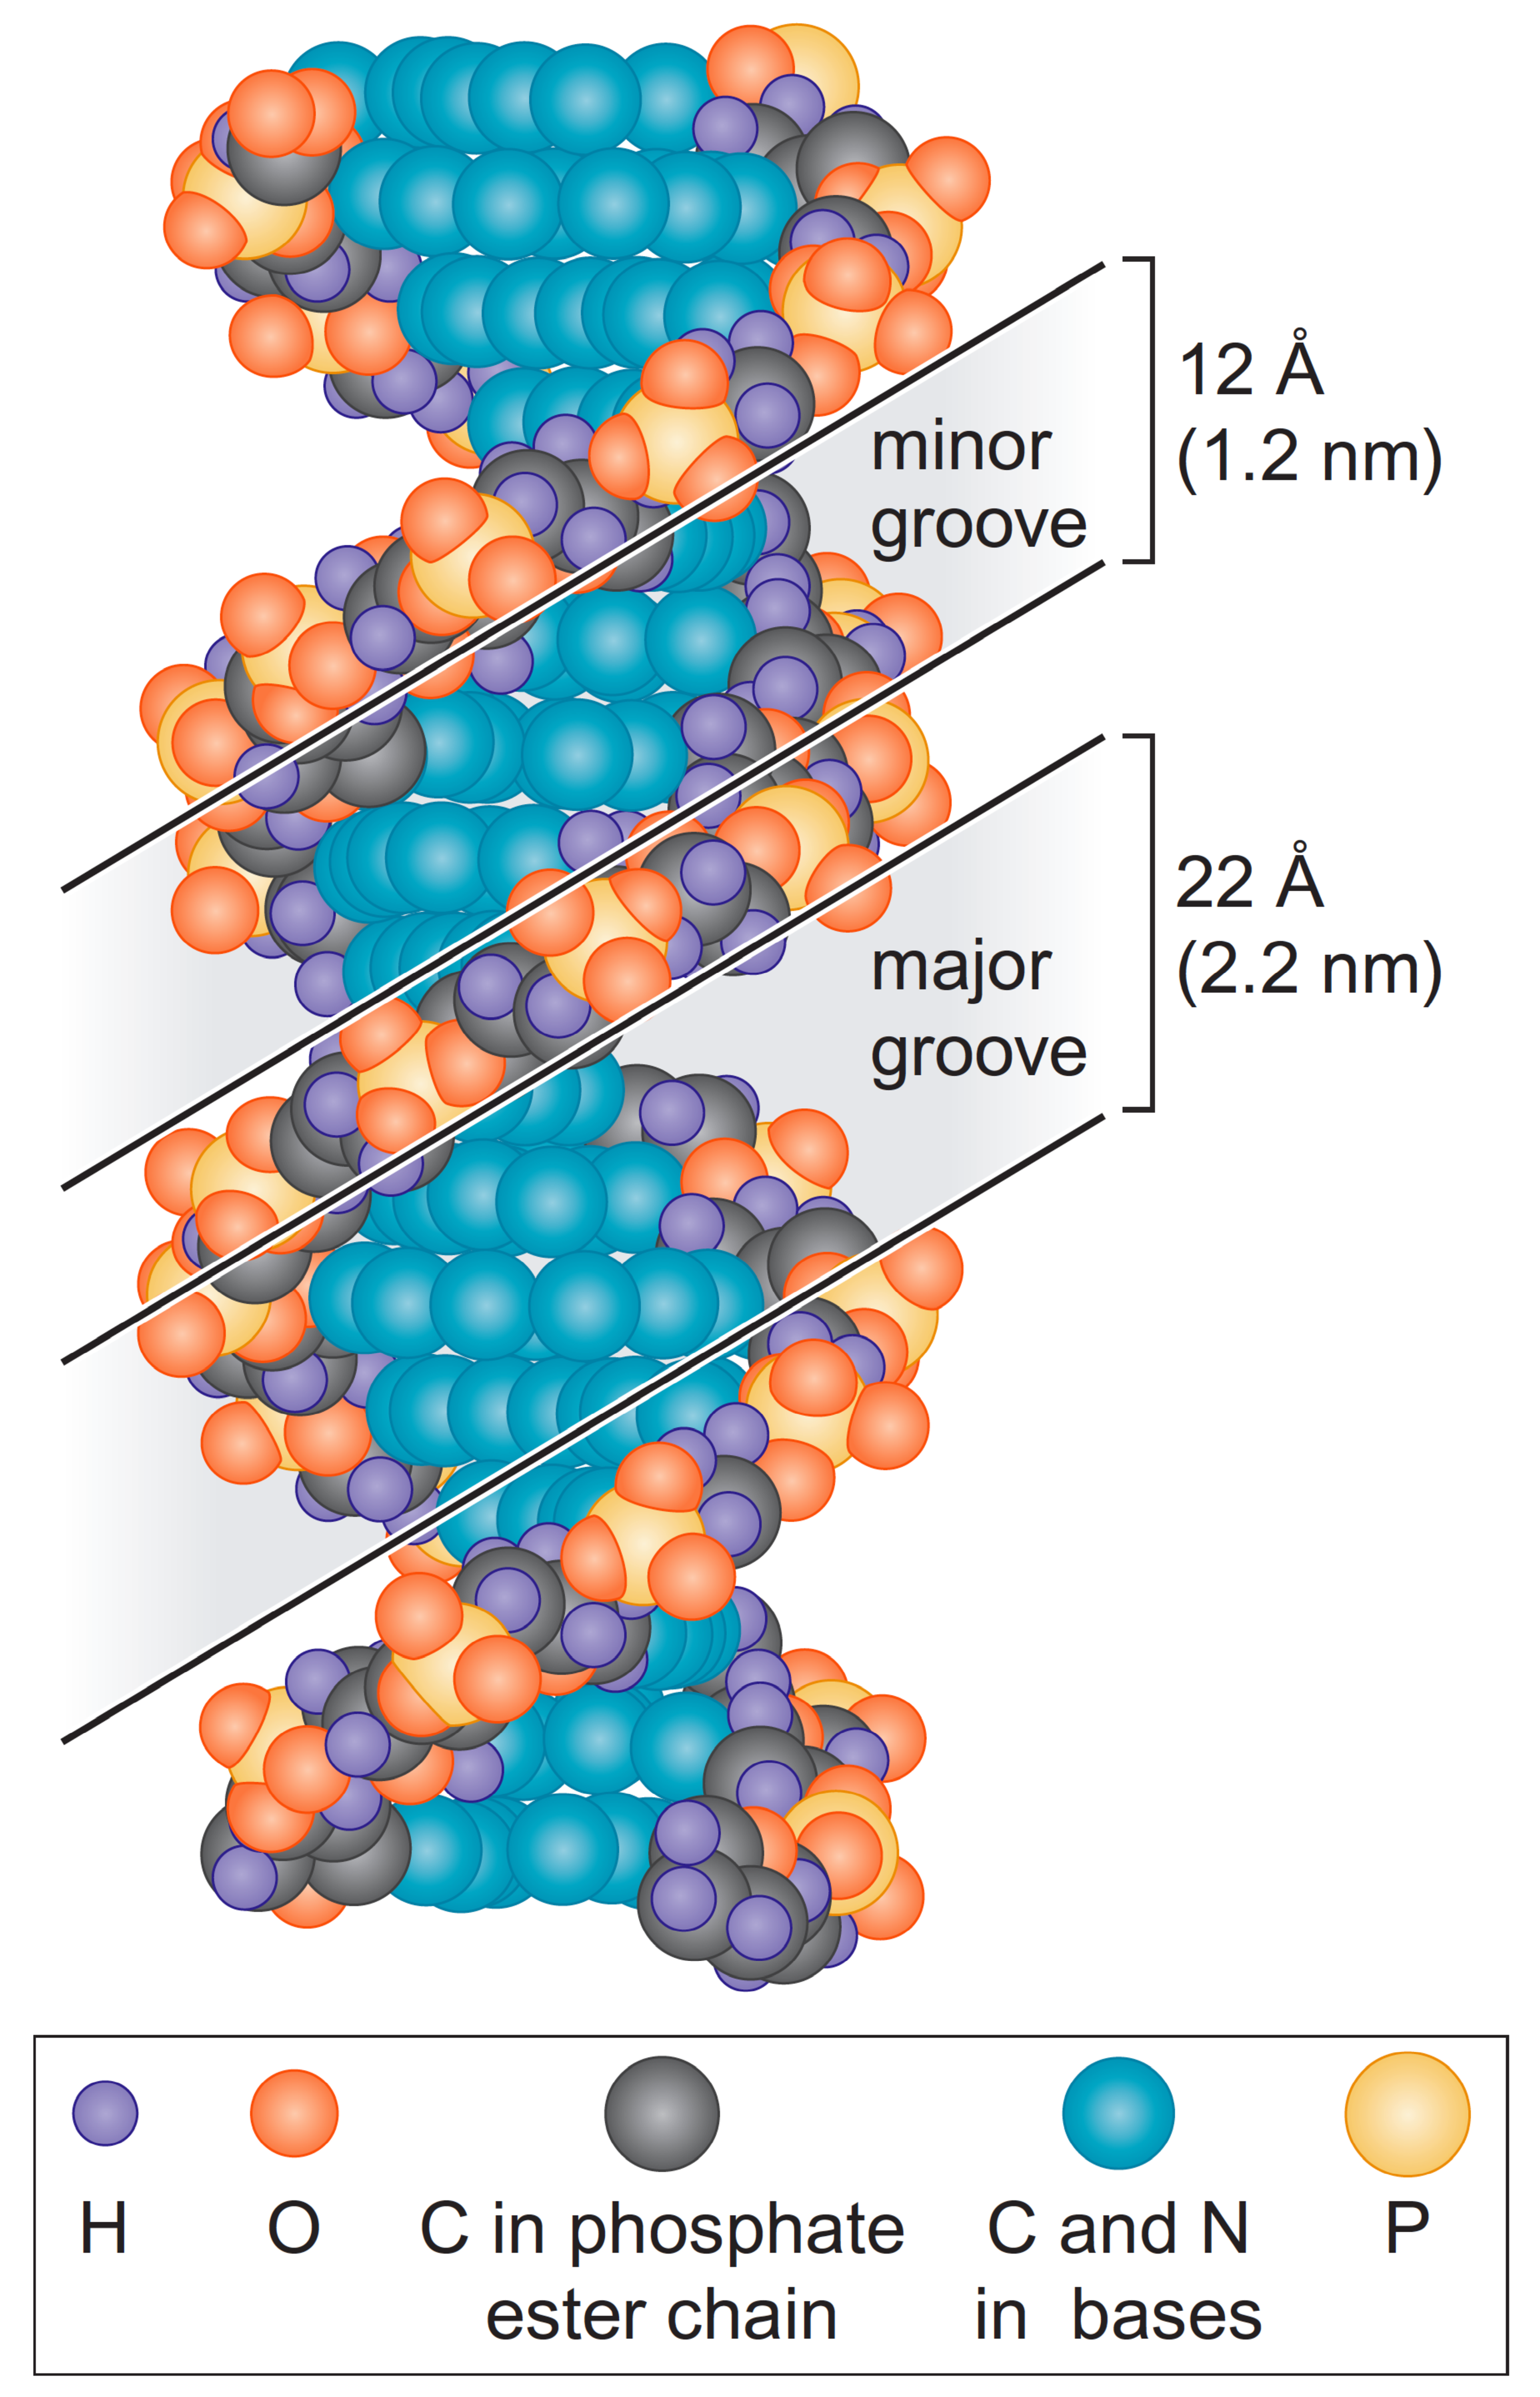
\includegraphics[width=0.4\textwidth]{Graphics/DNA/dna_space_filled.pdf}}
\caption{On the left is a schematic model of the double helix illustrating the base-pairs, and the sugar-phosphate backbone. The space-filled illustration on the right highlights the overall twist of the DNA structure with the bases located on the inside of the cylindrical structure. These illustrations are from figure 6-1 in reference \cite{Watson2003}.} 
\label{fig:dna_structure_filled}
\end{figure}
%
The first type of bases which contain two heterocyclic rings are classified as purines, called adenine (A) and guanine (G) (\figref{dna_purine}); the second type contain only a single heterocyclic ring and are classified as pyrimidines, called thymine (T) and cytosine (C) (\figref{dna_pyrimidine}). These bases participate in hydrogen bonding where two bases are connected by hydrogen bonds to form complimentary AT, and GC base-pairs. Both base-pairs have the same dimensions giving them the same planar geometry allowing the base-pairs to stack on top of each other without disturbing the sugar-phosphate backbones. The AT base-pairs are linked by two hydrogen bonds whereas the GC base-pairs are linked by three hydrogen bonds. Although individual hydrogen bonds are relatively weak when compared to covalent bonds, the bonding between the polynucleotides lies perpendicular to the fibre axis making the strength of the hydrogen bonds additive \cite{Berg2010,Watson2003}.
%
\begin{figure}[t]
\centering
\subfloat[]{\label{fig:dna_purine}\centering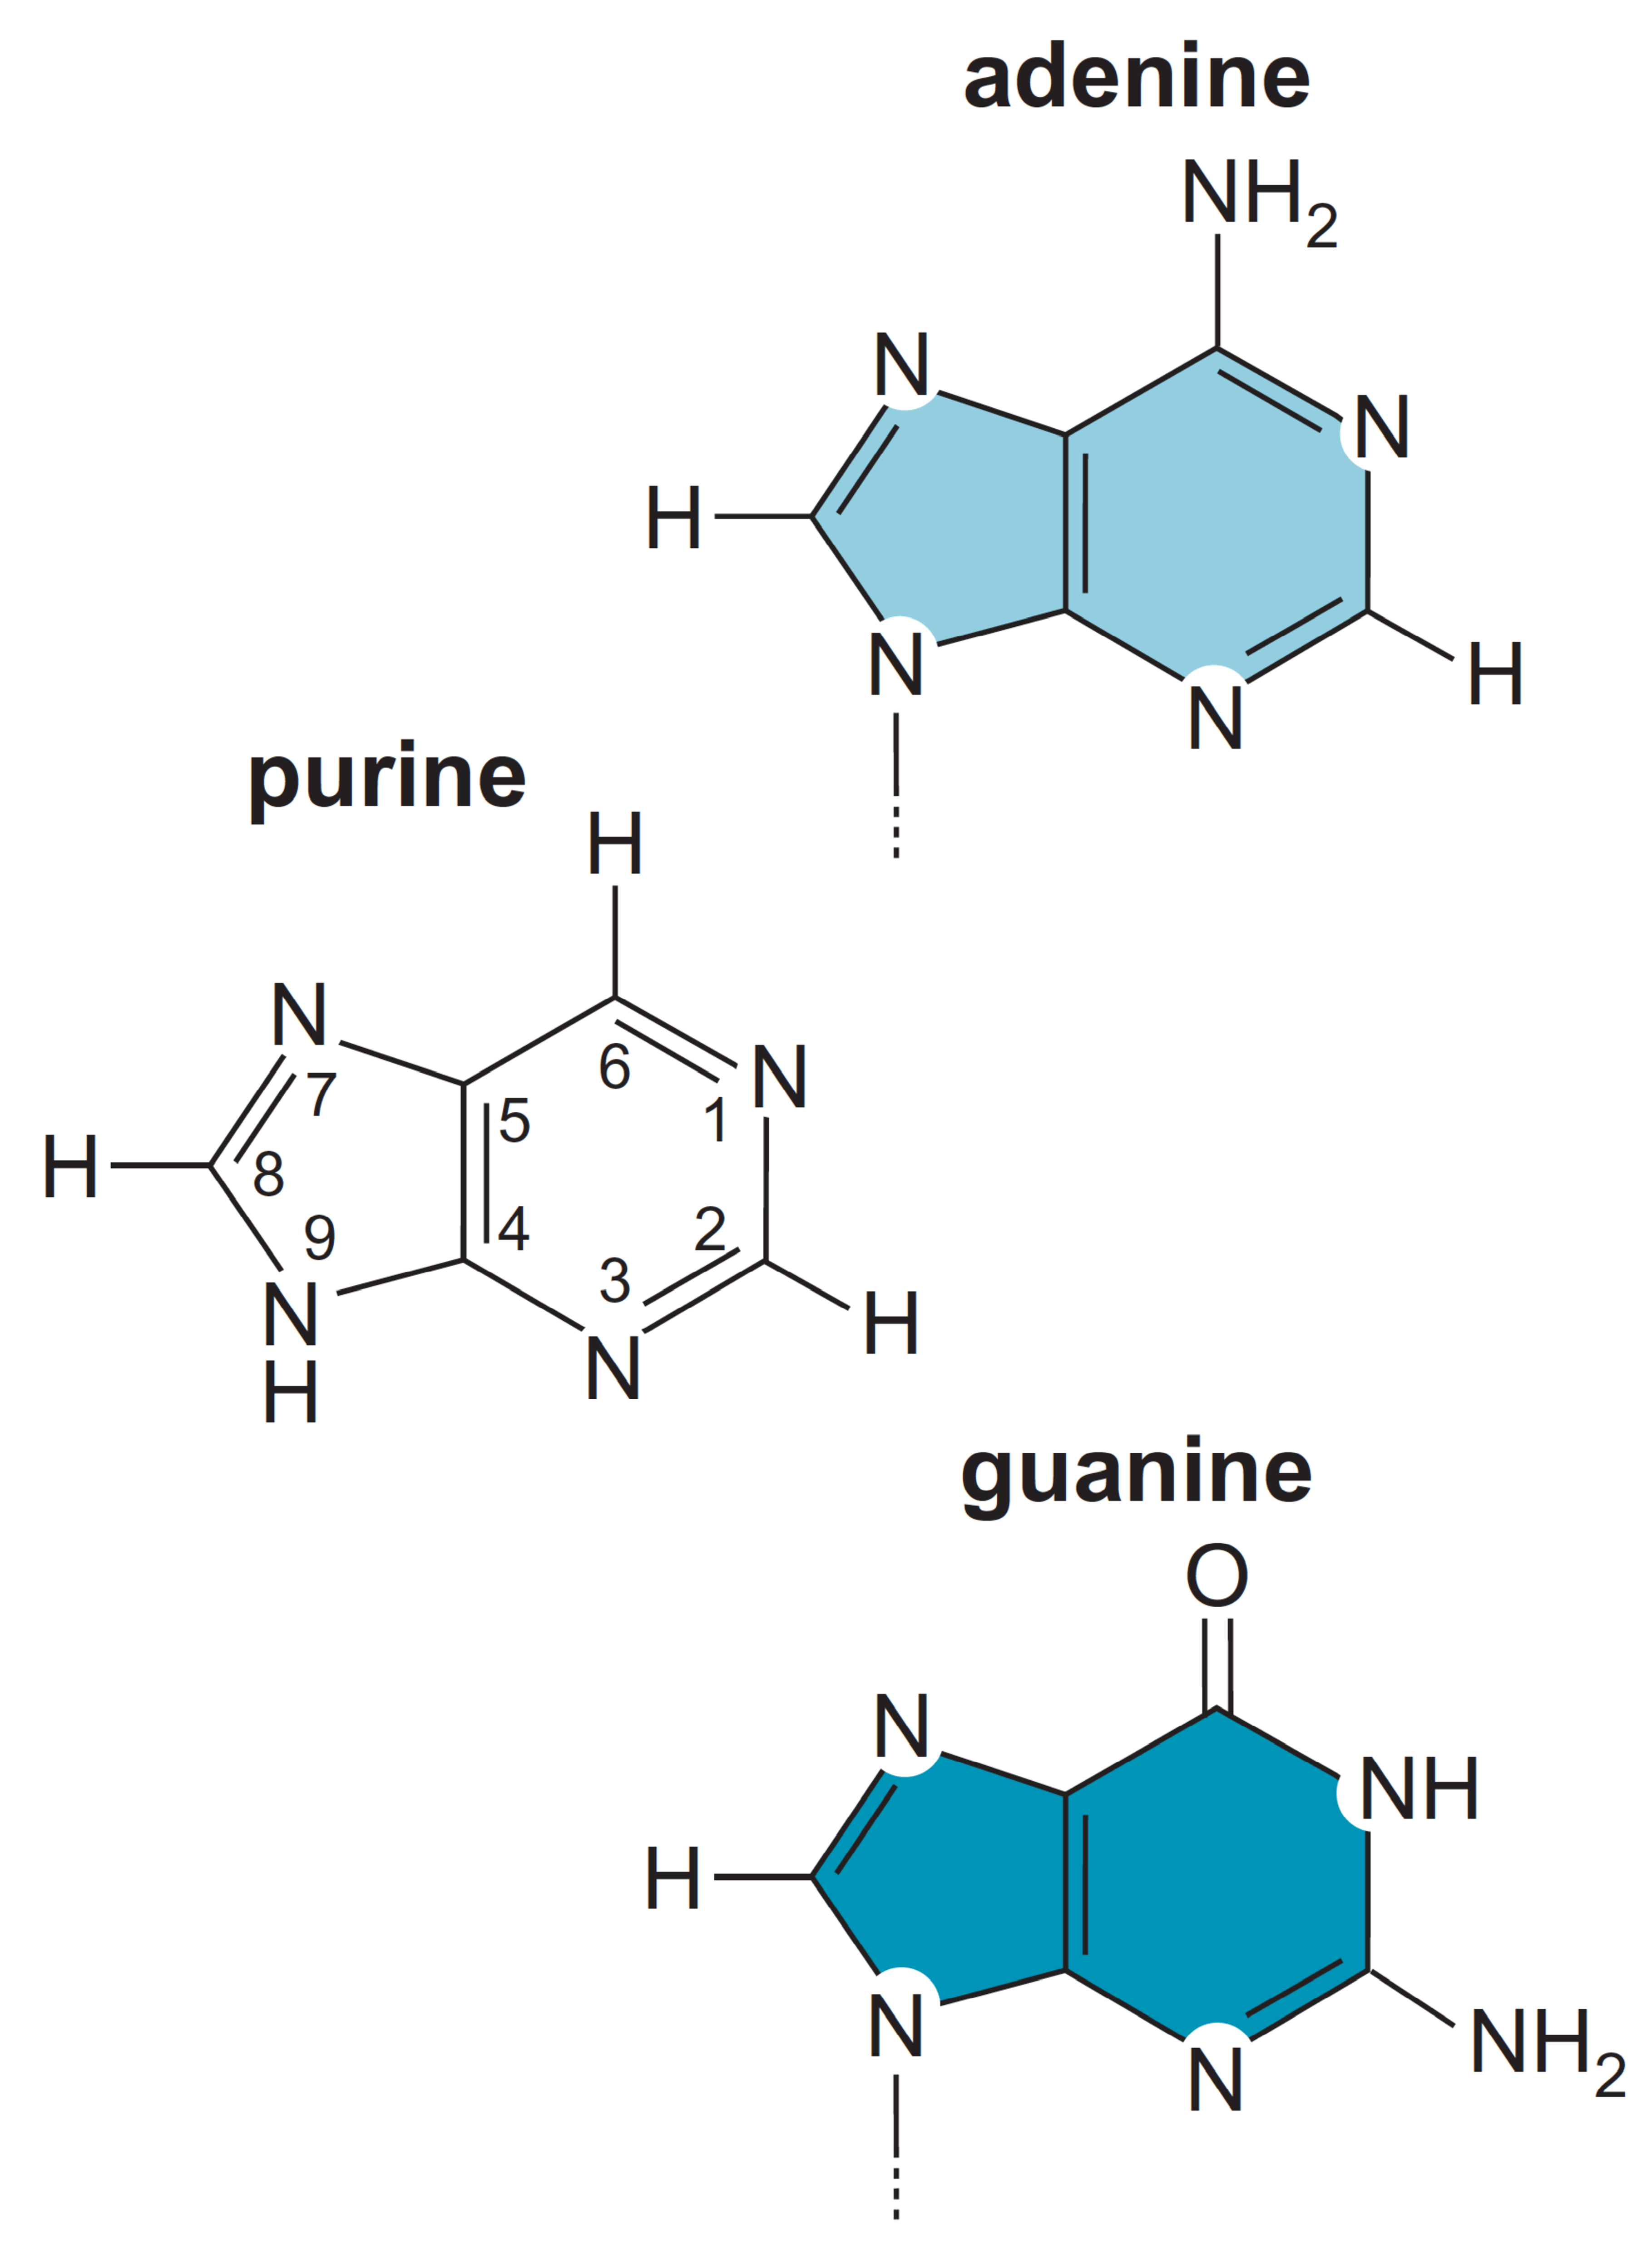
\includegraphics[width=0.3\textwidth]{Graphics/DNA/dna_purine.pdf}}
\hspace{20mm}         
\subfloat[]{\label{fig:dna_pyrimidine}\centering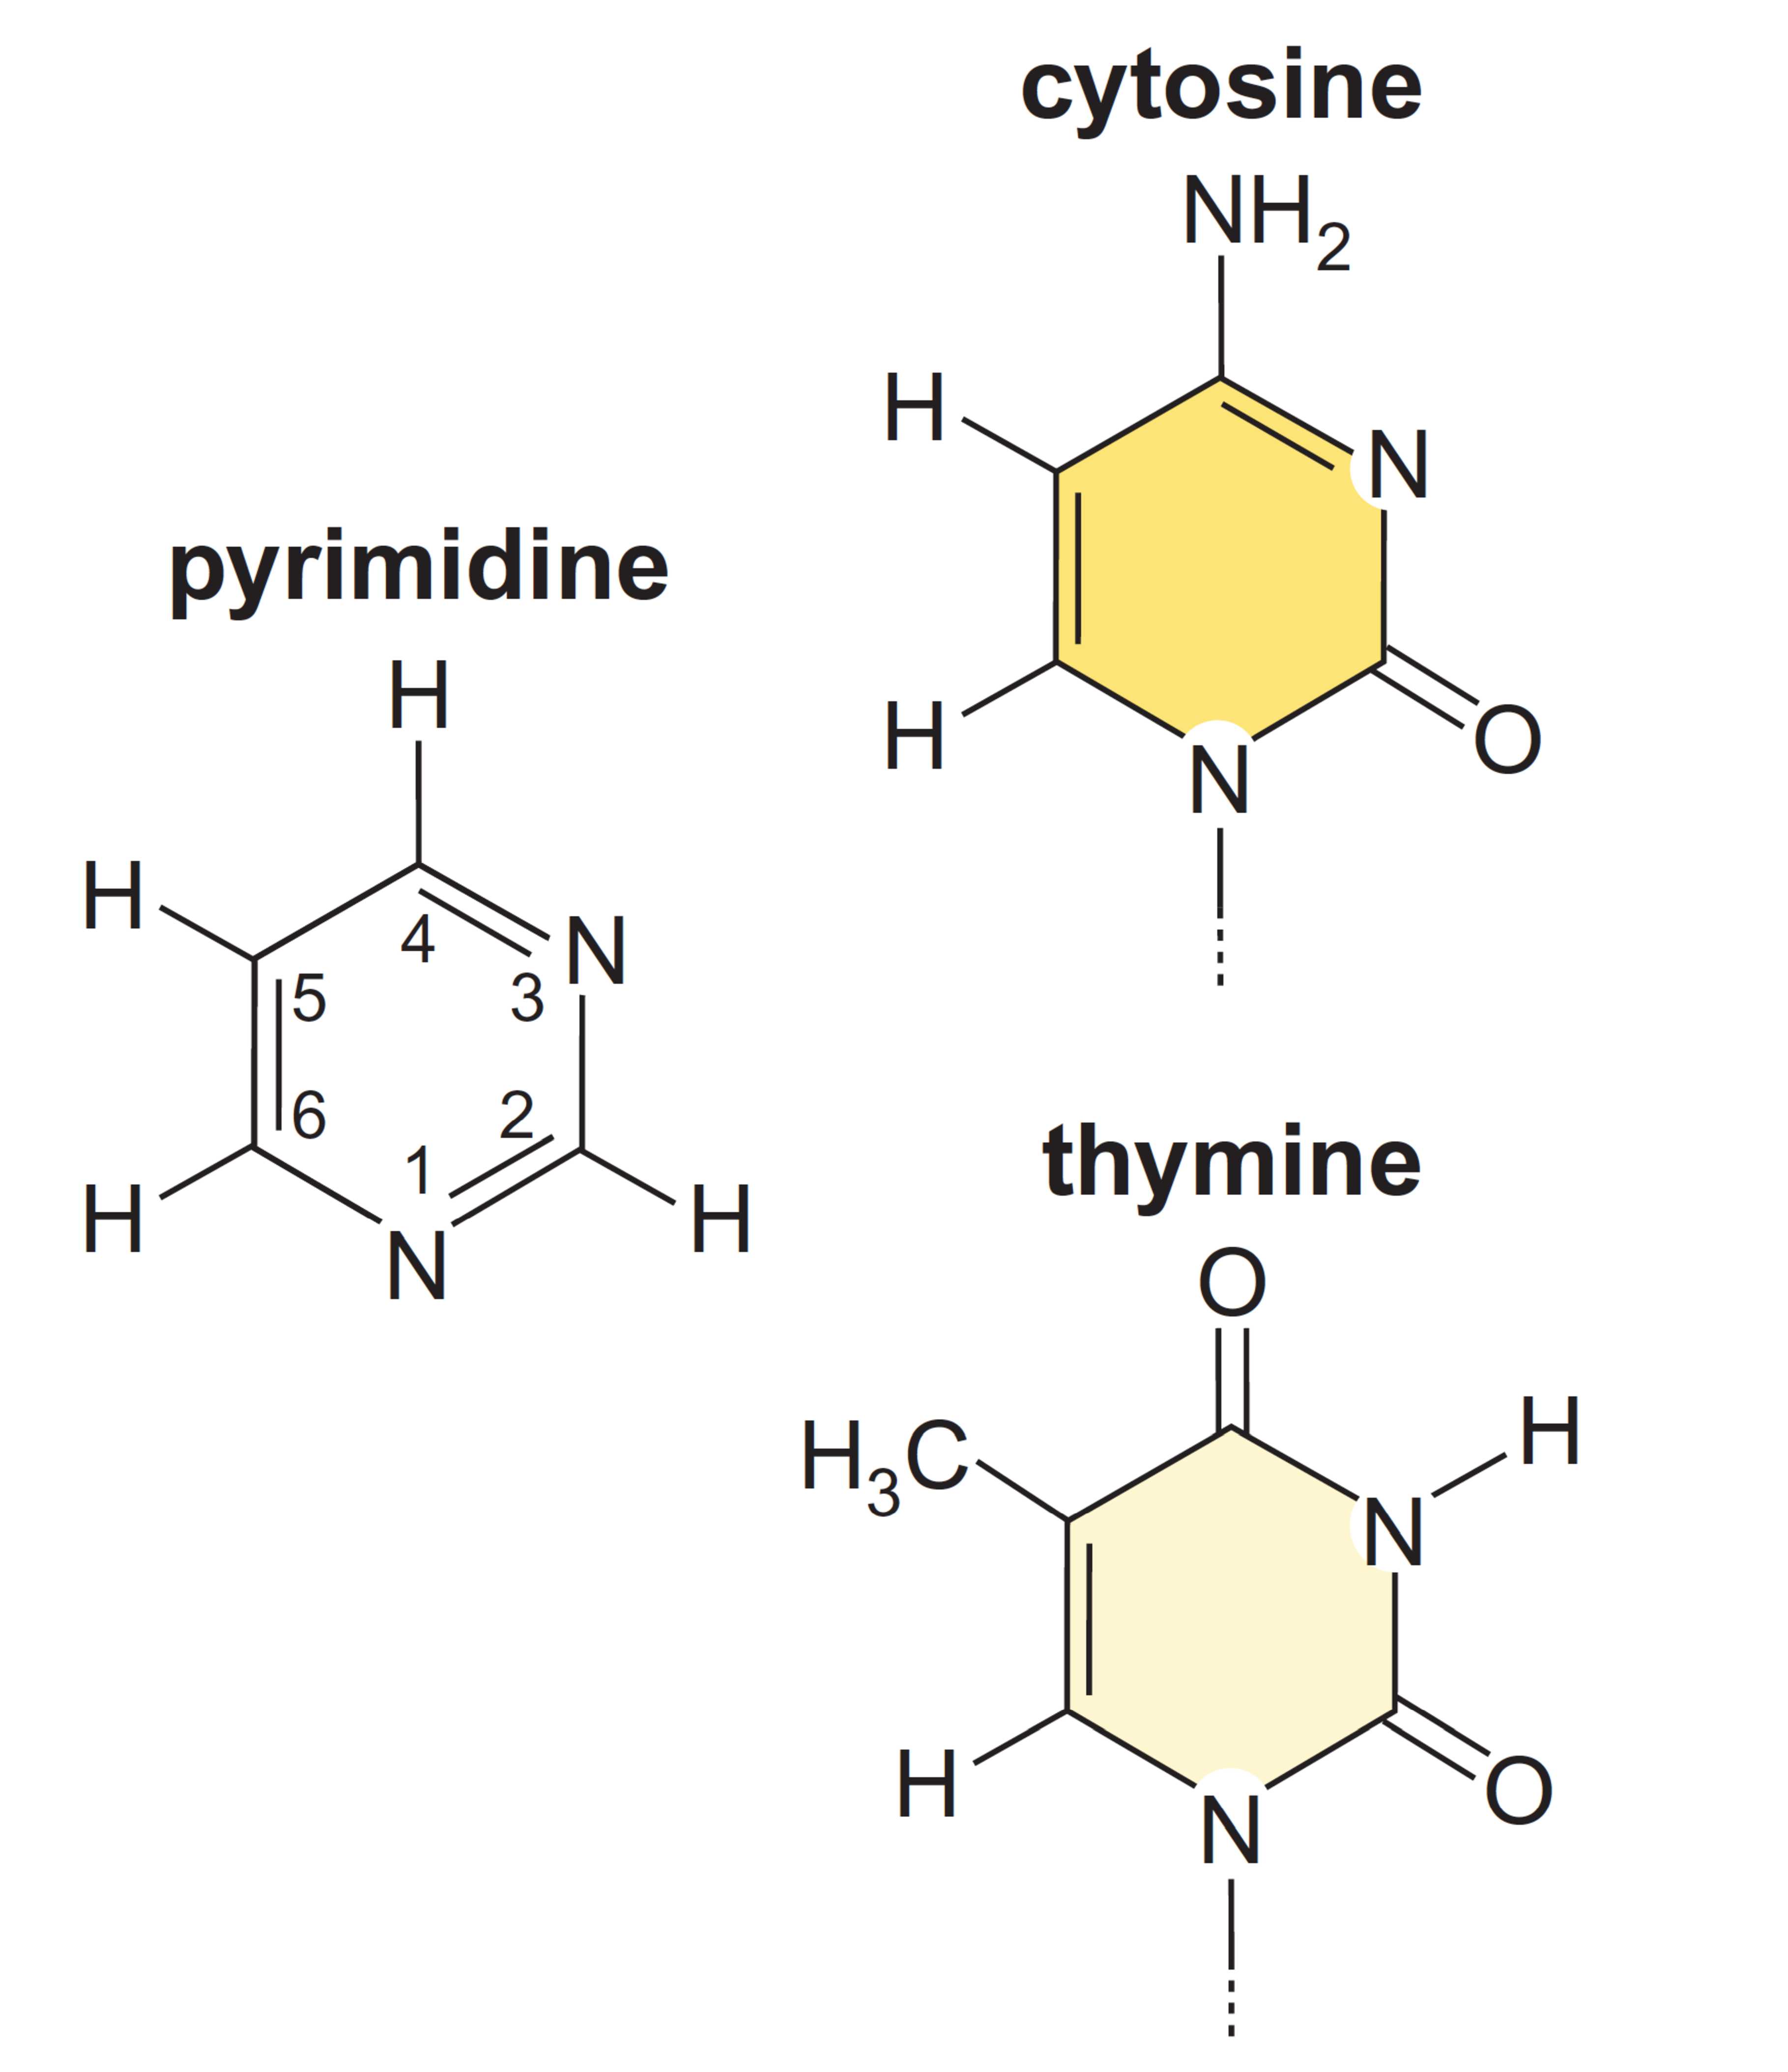
\includegraphics[width=0.3\textwidth]{Graphics/DNA/dna_pyrimidine.pdf}}
\caption{The types of bases that exist in DNA. On the left are the two purine bases that contain two heterocyclic rings, and on the right are the two pyrimidine bases that contain a single heterocyclic ring. These illustrations are from figure 6-1 in reference \cite{Watson2003}.} 
\label{fig:dna_bases}
\end{figure}
%
Although these hydrogen bonds may contribute to some of the stability of the double helix structure the main contribution comes from the stacking interaction between the bases. A combination of dipole-dipole interactions, $\pi$-$\pi$ stacking interaction, van der Waals forces and hydrophobic forces, produce an overall complex attractive interaction between the heterocyclic rings of the base-pairs. In its natural conditions, DNA is a right-handed double-helix which contains about 10.5 base-pairs per helical turn. It has two neighbouring base-pairs that are separated axially by 0.34 nm and the pitch length, the length of a helical turn of the double-helix along the central axis, is about 3.4 nm \figref{dna_structure} \cite{Watson1953}.
%
\begin{figure}[htp]
\centering
\subfloat[]{\label{fig:dna_AT_base_pair}\centering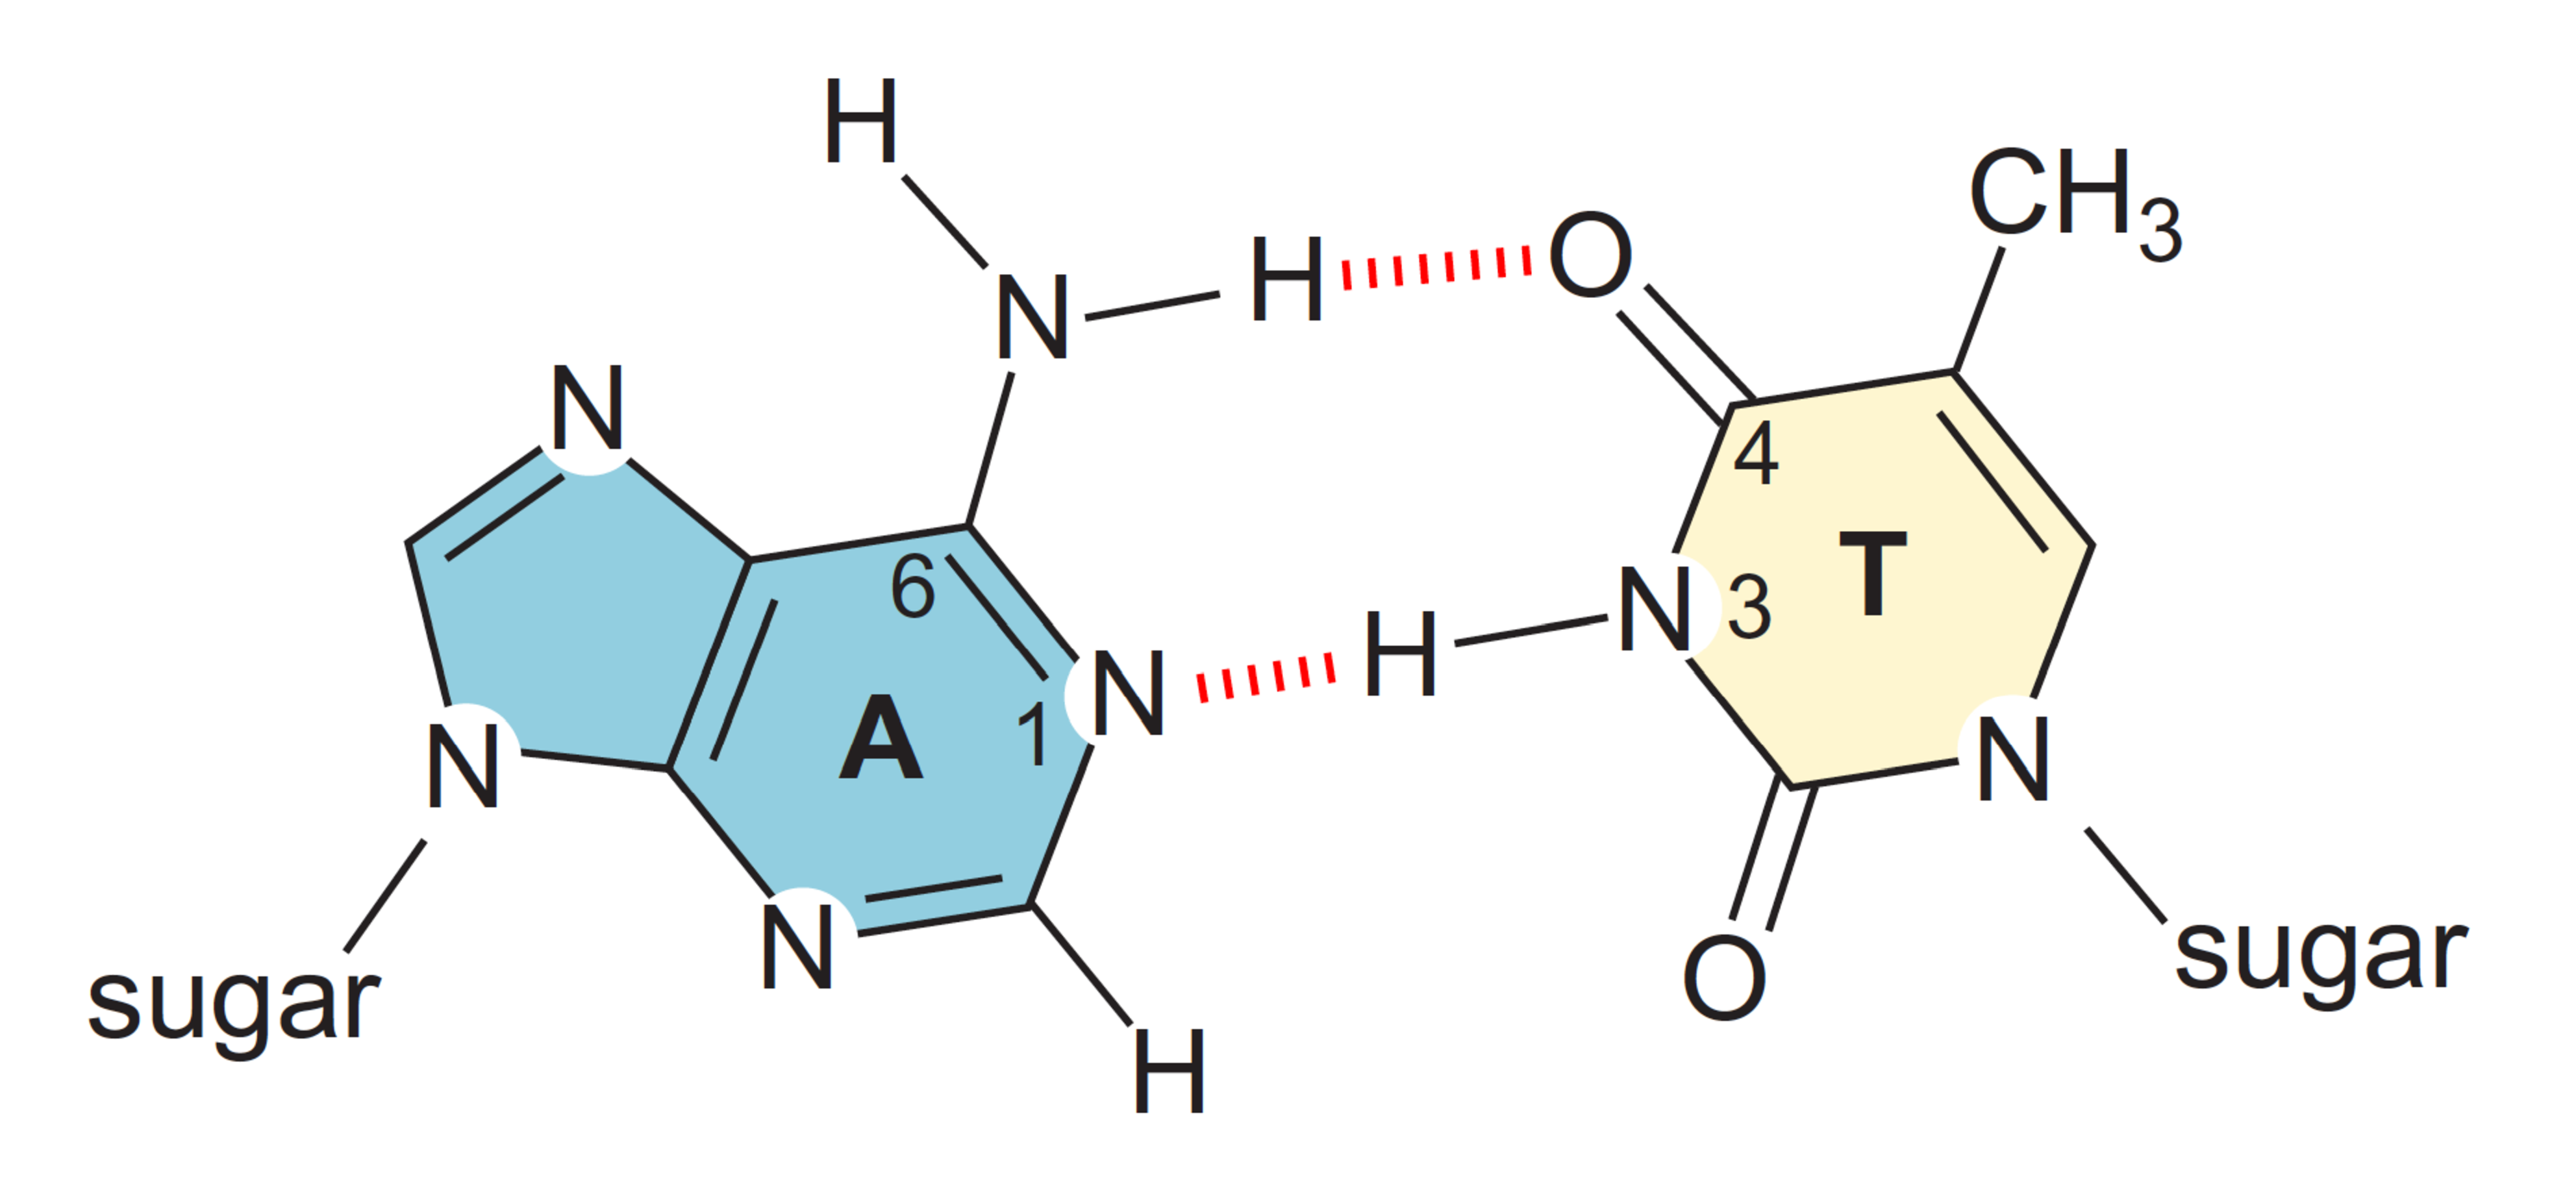
\includegraphics[width=0.4\textwidth]{Graphics/DNA/dna_base_pair_AT.pdf}}
\hspace{10mm}                
\subfloat[]{\label{fig:dna_GC_base_pair}\centering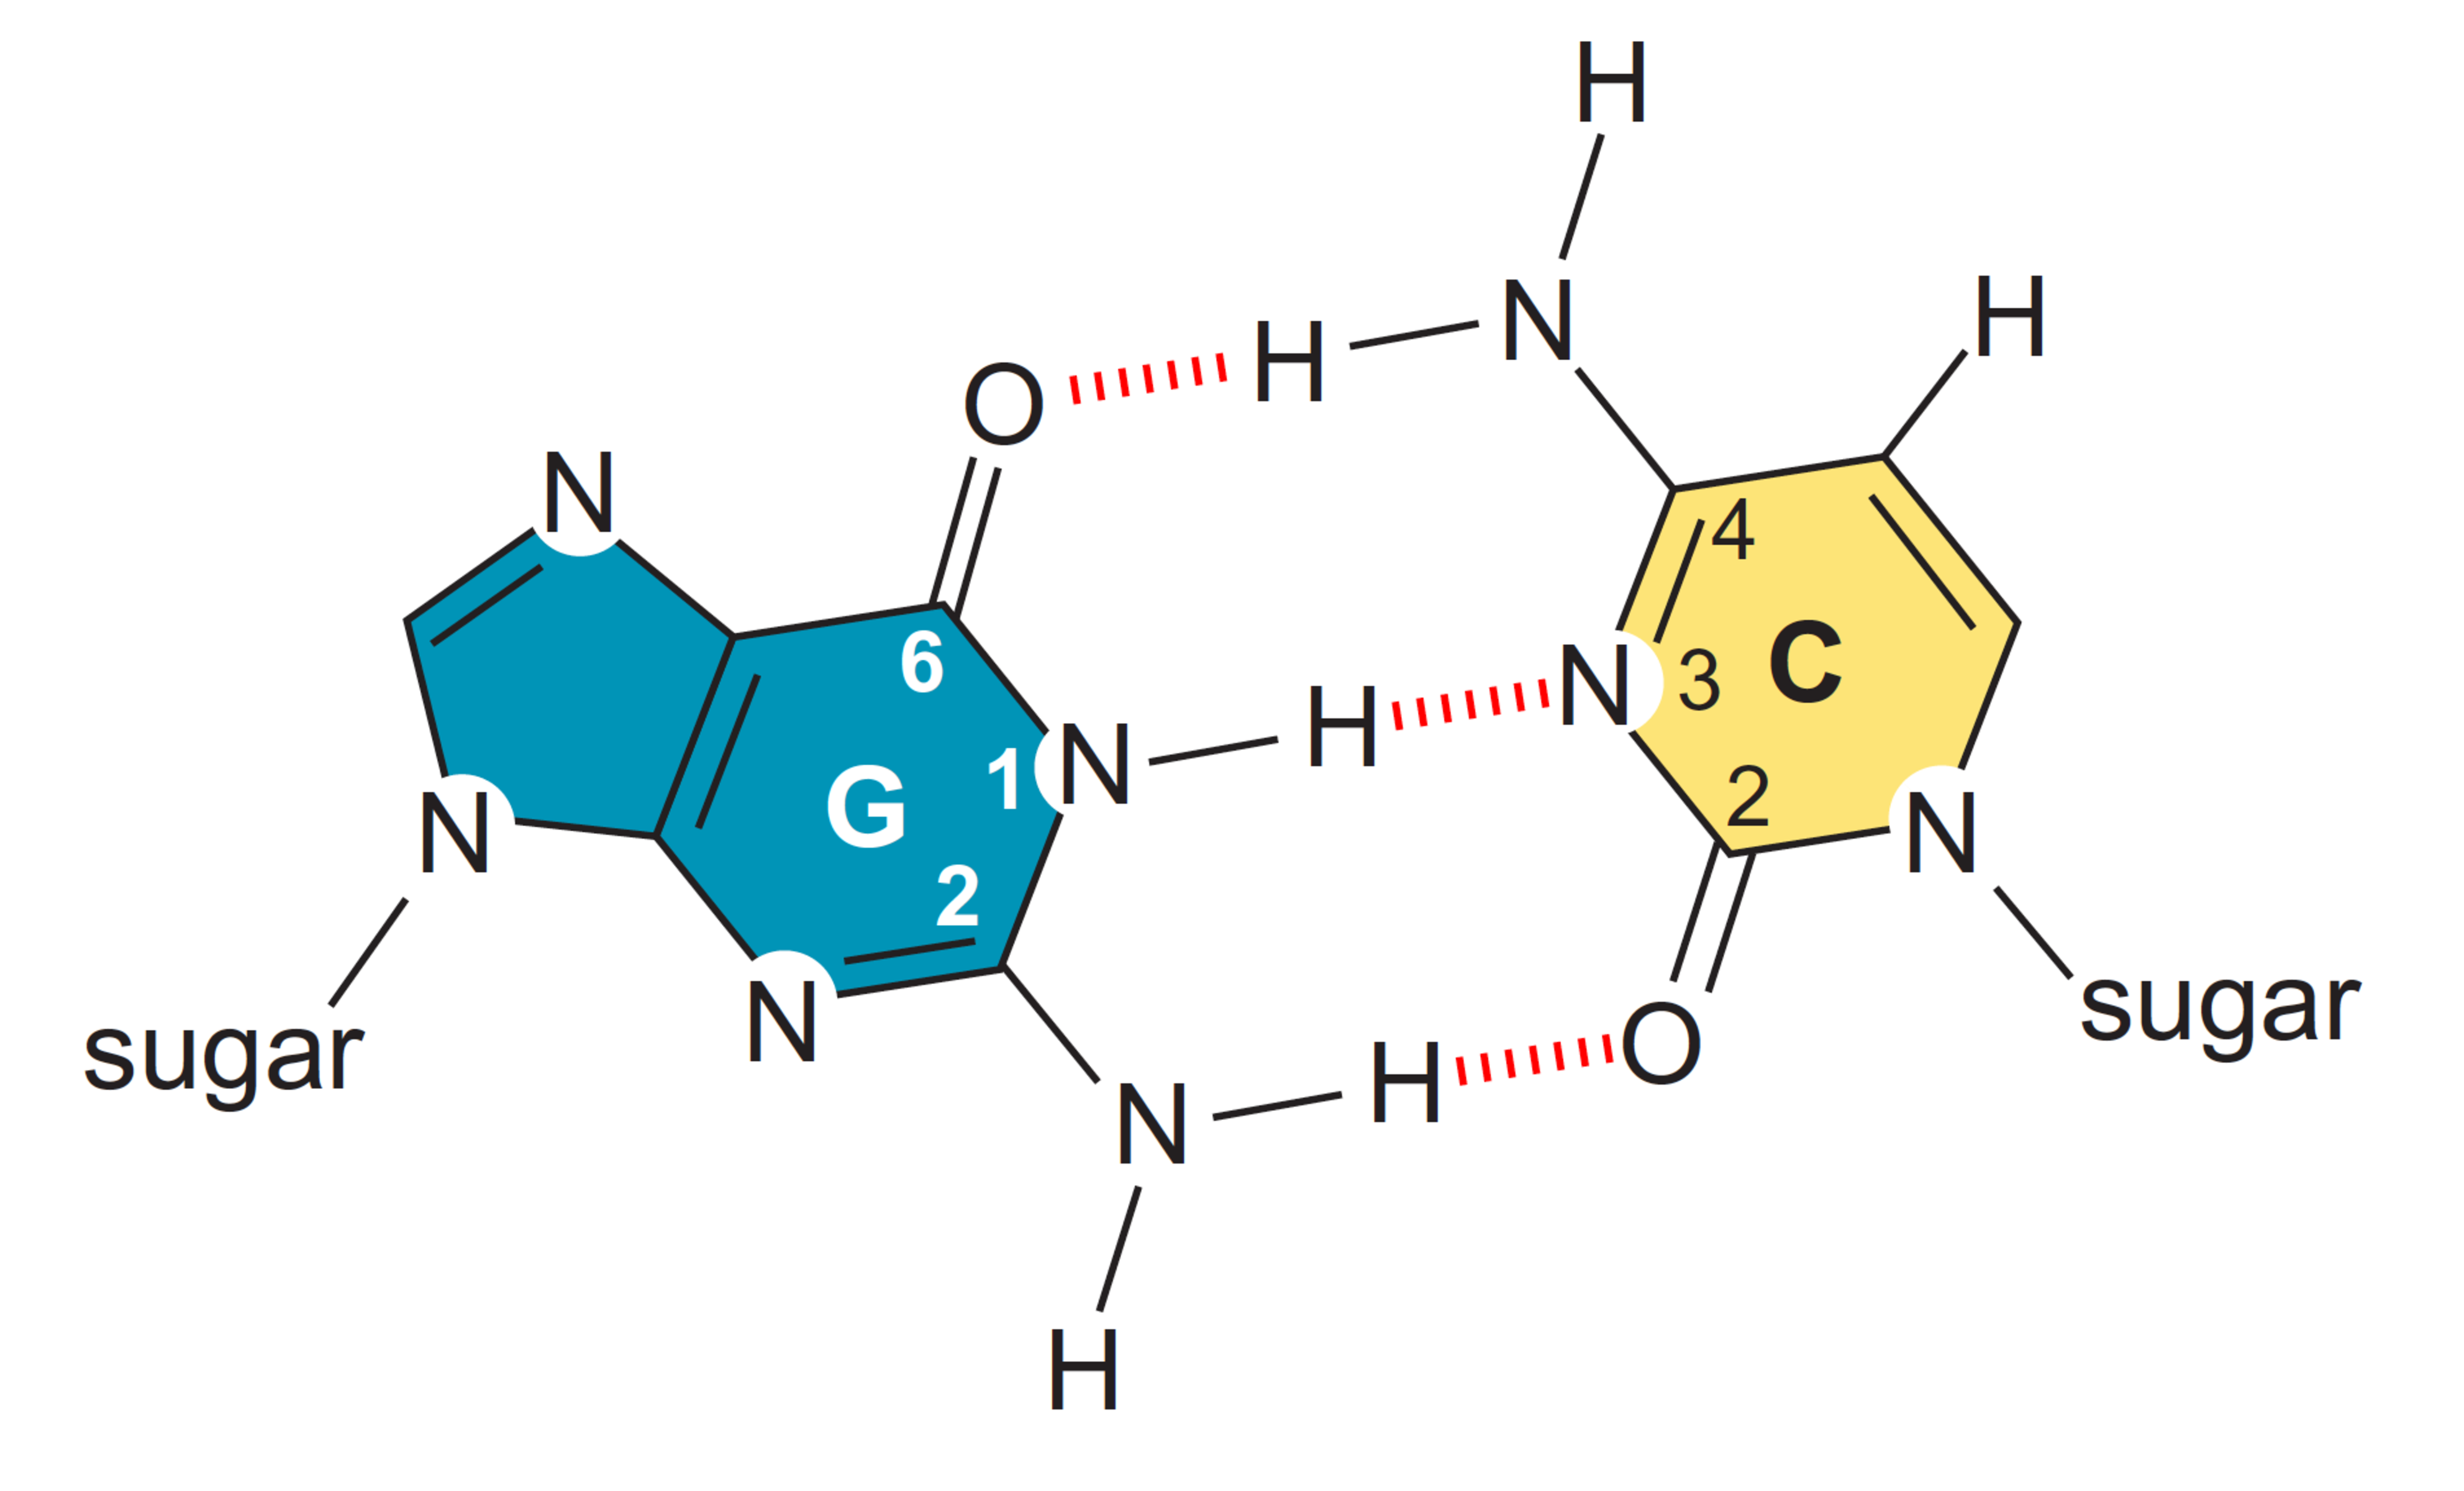
\includegraphics[width=0.4\textwidth]{Graphics/DNA/dna_base_pair_GC.pdf}}
\caption{Chemical structure of the complementary base-pairs in DNA. On the left is the adenine-thymine(AT) base-pair with two hydrogen bonds and on the right is the guanine-cytosine base-pair with three hydrogen bonds. These illiustrations are from figure 6-3 figure 6-6 in reference \cite{Watson2003}.} 
\label{fig:dna_base_pairs}
\end{figure}
%
\begin{figure}[htp]
\centering \includegraphics[scale=0.1]{Graphics/DNA/dna_schematic.pdf}
\caption{Another schematic diagram of the DNA molecule showing the different molecular groups within the backbone and base-pairs. This illustration is from figure 6-3 in reference \cite{Watson2003}.}
\label{fig:dna_schematic}
\end{figure}
%
\subsection{DNA Mechanics}

Double stranded DNA behaves like any other polymer in aqueous solution, exchanging energy with its surrounding environment at thermal equilibrium. The thermal agitation causes the DNA to bend and curve locally by small forces that continuously change the macroscopic configuration of the molecule. Commonly described as Brownian motion this has the effect of reducing the end-to-end distance of the molecule, maximising its conformational entropy such that its most probable configuration is a random coil. Purely entropic in origin, the free energies of deformations of the molecule are of order $kT \sim 4$ pN nm which sets the lower limit of the forces needed to stretch a DNA molecule to its contour length \cite{Harris2004,Strick2003}. 

Some of the first experiments measuring the entropic elasticity of DNA were conducted by Smith et al (1992). Using a method where they chemically attached one end of the DNA to a glass surface and tethered the other end to a magnetic bead they were able to measure the force extension of DNA using a combination of magnetic fields and hydrodynamic drag \cite{Smith1992}. The results shown from their experiments in \figref{fig1_Bustamante2000} describe DNA having a linear relationship in the limit of low forces with a Hooke's constant that is inversely proportional to the length of the molecule. Here we see the FJC model agreeing well with such force extension curves for DNA. As the applied force increases the experimental results clearly dismiss the FJC model as a suitable candidate for describing DNA.

A better description is provided by the Worm Like Chain (WLC) model which considers DNA to be a continuous flexible worm-like chain \cite{Marko1995}. In this model the persistence length $L_{p}$ is a quantitative measure of chain stiffness which defines a length scale over which segments of the counter length are correlated. Since the FJC model is only flexible between fixed segments and ignores the bending fluctuations of the segments themselves, the WLC provides a more realistic description of entropy change in stiffer polymers. 
%
\begin{figure}[h]
\centering
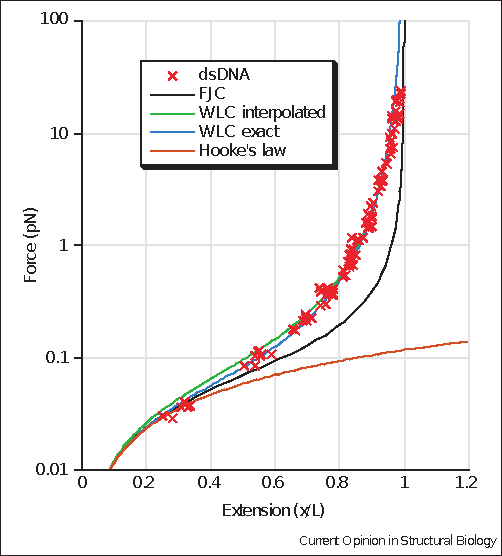
\includegraphics[scale=1]{Graphics/DNA/fig1_Bustamante2000.pdf}
\caption{Force extension behaviour of double stranded DNA. The experimental data taken from Smith et al. (1992) is fitted to the WLC model using the modified WLC interpolated formula \eqref{wlc_num_approx}, the exact WLC model solved numerically, and the linear spring \eqref{wlc_num_approx_small} are also shown. In these plots $L_{p}=53$ nm where the FJC assumes twice the persistence length. This original plot was reported in \cite{Bustamante2000}.}
\label{fig:fig1_Bustamante2000}
\end{figure}
%
The first complete treatment of the WLC model was achieved by Marko and Siggia using two different methods; for the exact solution they numerically evaluated a line integral of two terms in the WLC model where the first term described the resistance of the chain bending, and the second term described the stretching energy resulting from an applied force. Following the terminology used in \cite{Marko1995} we describe the DNA conformations by a space curve $\mathbf{r}(s)$ of a contour length, $L$, where $s$ is the arc length, and the energy in the WLC model is expressed as:
%
\begin{equation}
E_{wlc}=k_{B}T \int_{0}^{L}ds \left(  \frac{A}{2}\left|\frac{d\mathbf{r}\left(s\right)}{ds}\right|^{2} -F\cos\left(\theta\left(s\right)\right)\right)
\end{equation}
%
where $\theta\left(s\right)$ is the angle between $\mathbf{r}(s)$ and the axis along the direction of force $F$.  In the second method they expanded the first term to the quadratic order that led to the Gaussian approximation of the line integral. They were able to derive an interpolation formula that was close to the exact numerical solution of the force-extensions  \cite{Marko1995,Bustamante1994}:
%
\begin{equation}
\label{wlc_num_approx}
F\left(x\right)=\left(\frac{k_{B}T}{L_{p}}\right)\left[\frac{1}{4\left(1-\frac{x}{L}\right)^{2}}-\frac{1}{4}+\frac{x}{L}\right]
\end{equation}
%
where $L$ is the length of the molecule, $L_{p}$ is the persistence length and $x$ is the extension. For small values of $\frac{x}{L}$, the approximation simplifies to
%
\begin{equation}
\label{wlc_num_approx_small}
F\left(x\right)=\frac{3 k_{B}T}{2L_{p}}\left(\frac{x}{L}\right)
\end{equation}
%
which demonstrates that the molecule behaves as a linear spring with a stiffness constant $k_{DNA}=\frac{3 k_{B}T}{2LL_{p}}$. Further corrections, and improvements have been made to \eqref{wlc_num_approx} to include effects of stretching DNA in physiological buffer \cite{Wang1997,Bouchiat1999}. For the results shown in \figref{fig1_Bustamante2003} the stretch modulus was found to be approximately 1000 pN in a buffer solution \cite{Bustamante2000}. The failure to account for the enthalpic correction at small forces (5-10 pN) leads to underestimation of $L_{p}$ resulting in a deviation from the model above 10 pN \cite{Bouchiat1999,Wang1997}. The experimental results shown in \figref{fig1_Bustamante2000} were taken from Smith et al. (1992) where the persistence length of DNA in the WLC model was $L_{p}\sim$ 53 nm in order to fit the experimental data. Other experiments including the more recent experiment by Van Maneren et al. (2009) have reproduced these force extension curves for DNA which have shown that the predictions of the WLC model provide an excellent agreement with the data measured \cite{Cluzel1996,Wang1997,Smith1996,VanMameren2009}. This can also be observed in \figref{fig1_Bustamante2000}. 
%
\begin{figure}[htp]
\centering
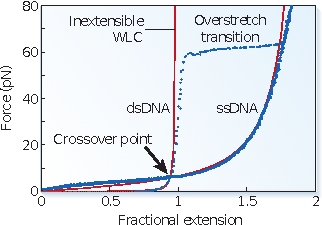
\includegraphics[scale=1.5]{Graphics/DNA/fig1_Bustamante2003.pdf}
\caption{Force extension behaviour of DNA and ssDNA \cite{Bustamante2003}. }
\label{fig:fig1_Bustamante2003}
\end{figure}
%
At forces above 65 pN DNA structurally changes under mechanical stress causing the DNA molecule to extend 1.7 times the original length. We see this extra length being released over a narrow range of force shown by the plateau in \figref{fig1_Bustamante2003}. Experiments have highlighted that the force at which the over-stretching transition occurs is dependent on the details of terminal attachments, $\sim 65$ pN if the molecule is torsionally relaxed at both ends, and $\sim 110$ pN if it is not. Two competing models \cite{VanMameren2009} have been proposed to describe the structural behaviour in this overstretched region: In the first model it is thought that DNA gradually unwinds under tension, with the base-pairs intact, into the S-form DNA resembling a parallel ladder.  The second model interprets the overstretched phase as a denatured DNA resulting from strand separation caused by breaking of hydrogen bonds between complementary bases. Recent experiments show that there is a region where both these models can coexist with base-pair melting causing strand separation from DNA to single stranded DNA (ssDNA) \cite{VanMameren2009,Williams2009,Fu2010}. 

\subsection{DNA Models}

In an attempt to study the DNA transcription process Peyrard et al. \cite{Peyrard1989a} found that developing a mathematical model that included the roles played by the RNA polymerase enzymes would be far too complex a task. Similarities were noted with DNA thermal denaturation, a mechanism where the backbone DNA strands separate by heating, also known as DNA melting. This function initiates locally by the formation of bubbles within the DNA structure and therefore was considered to be a preliminary step in understanding the transcription process \cite{Peyrard1989a, Dauxois1993a, Dauxois1993, Peyrard2004}. 

Simplifying the DNA structure to a 1D ladder system Peyrard et al. were able to write a  Hamiltonian as a function of base pair separation that included temperature independent parameters, and then studied the statistical mechanics of the system by employing the transfer integral method. The model has two degrees of freedom where in each strand the displacements of the $n^{th}$ base from their equilibrium position is labelled $u_{n}$ and $v_{n}$ along the direction of the hydrogen bond that connects base pair. The structure is considered homogeneous and periodic with each nucleotide base being represented by a point mass $m$ \cite{Peyrard1989a}.

The effective base pair potential $V$ was modelled by a Morse potential to represent the 2 or 3 hydrogen bonds that connect the two bases in a pair, and along each backbone  strand the neighbouring bases are connected by a stacking harmonic potential that has a stiffness constant $\kappa$. For system with $N$ base pairs, the Hamiltonian is expressed as \cite{Peyrard1989a},
%
\begin{equation}
H=\sum_{n}\frac{m}{2}\left( \dot{u}_{n}^{2} + \dot{v}_{n}^{2}  \right) +\frac{\kappa}{2}\left(u_{n}-u_{n-1}\right)^{2} + \frac{\kappa}{2}\left(v_{n}-v_{n-1}\right)^{2}+V \left(u_{n}-v_{n}\right)
\label{pb_model_hamiltonian}
\end{equation}
%
with
%
\begin{equation}
V \left(u_{n}-v_{n}\right) = D\left[\exp \left(-a\left( u_{n}-v_{n} \right) \right) -1\right]^{2}
\label{pb_model_bp_potential}
\end{equation}
%
where $D$ is the dissociation energy of the base pair, and $a$ is the parameter that sets the spatial range of the base pair potential. The first term in \eqref{pb_model_hamiltonian} represents the kinetic energy of the system, the second term corresponds to the effect of stretching along the backbone, and the third term represents the interaction of the base pair. 

Further simplifications are made to the Hamiltonian by transforming the co-ordinate system into variables that represent the in-phase $x_{n}$, and out-of-phase $y_{n}$ motions of the base positions. The transformations are \cite{Peyrard1989a}
%
\begin{equation}
x_{n}=\frac{u_{n}+v_{n}}{\sqrt{2}}
\end{equation}
%
\begin{equation}
y_{n}=\frac{u_{n}-v_{n}}{\sqrt{2}}
\end{equation}
%
which readily separates the Hamiltonian to give 
%
\begin{equation}
H = H\left(x_{n}\right) + H\left(y_{n}\right)
\end{equation}
%
with 
%
\begin{align}
H\left(x\right) &= \sum_{n}\frac{p_{n}^{2}}{2m}+\frac{\kappa}{2}\left(x_{n}-x_{n-1}\right)^{2} \\
H\left(y\right) &= \sum_{n}\frac{q_{n}^{2}}{2m}+\frac{\kappa}{2}\left(y_{n}-y_{n-1}\right)^{2} + V'\left(y_{n}\right)
\end{align}
%
where $p_{n}=m\dot{x}_{n}$, $q_{n}=m\dot{y}_{n}$ and $V'\left(y_{n}\right)=V\left(\sqrt{2}y_{n}\right)$. In the partition function integral we find that the momentum terms and the terms in $x_{n}$ integrate analytically to provide a constant factor in the total partition function. For the remaining terms in $y_{n}$ the partition function integral can be written as  \cite{Peyrard1989a}
%
\begin{equation}
Z\left(\beta\right)=\int \prod^{N}_{n=1} \,dy_{n}\exp\left(-\beta H\left(y_{n},y_{n-1}\right) \right)\delta\left(y_{N}-y_{1}\right)
\label{pfi1}
\end{equation}
%
with the delta function fulfilling a periodic boundary condition.  This partition function integral can also be expressed using a product of Boltzmann factors to give
%
\begin{equation}
Z\left(\beta\right)=\int \prod^{N}_{n=1} \,dy_{n}\left[ \prod_{i=1}^{N}\exp\left(-\beta f\left(y_{n},y_{n-1}\right) \right)\right]\delta\left(y_{N}-y_{1}\right)
\label{pfi2}
\end{equation}
%
where the term $f\left(y_{n},y_{n-1}\right)$ can be generalised to a sum of the backbone interactions $W\left(y_{n},y_{n-1}\right)$ and the base pair interactions $V'\left(y_{n}\right)$, that is,
%
\begin{equation}
f\left(y_{n},y_{n-1}\right)= W\left(y_{n},y_{n-1}\right) +V'\left(y_{n}\right) = \frac{\kappa}{2}\left(y_{n}-y_{n-1}\right)^{2} + V'\left(y_{n}\right)
\end{equation}
%
In this one-dimensional problem the integral can be evaluated exactly in the thermodynamic limit of a large system using the eigenvalues and eigenfunctions of a transfer matrix. Introducing the the transfer integral operator $T$ we have an eigenvalue equation \cite{Peyrard1989a}
%
\begin{equation}
\int dy' T\left(y,y'\right)\psi_{i}\left(y'\right) =\lambda_{i}\psi_{i}\left(y\right)
\end{equation}
%
with
%
\begin{equation}
T\left(y,y'\right) = \frac{\kappa}{2}\left(y-y'\right)^{2} + V'\left(y\right)
\end{equation}
%
where $\psi_{i}$ are the orthonormal eigenfunctions and $\lambda_{i}$ are the corresponding eigenvalues. From \eqref{pfi2} the delta functions are expanded as a set of orthonormal eigenfunctions $\delta\left(y_{N}-y_{1}\right) = \sum_{i}\psi^{*}_{i}\left(y_{N}\right)\psi_{i}\left(y_{1}\right)$, such that the partition function now becomes
%
\begin{align}
Z\left(\beta\right)=& \sum_{i}\int dy_{1}\exp\left(-\beta f\left(y_1,y_2\right)\right)\psi_{i}\left(y_1\right)\int dy_{2}\exp\left(-\beta f\left(y_2,y_3\right)\right)\nonumber\\
&...\int dy_{N-1}\exp\left(-\beta f\left(y_{N-1},y_{N}\right)\right)\psi^{*}_{i}\left(y_N\right)
\label{pfi3}
\end{align}
%
Using the eigenvalue equation we can contract the integrals to give a reduced form of the partition function equation that is a sum over all eigenvalues \cite{Peyrard1989a}
%
\begin{equation}
Z\left(\beta\right)=\sum_{i}\lambda^{N-1}_{1}
\end{equation}
%
In the limit of a large DNA structure the largest eigenvalue $\lambda_{1}$ dominates from the contractions. The free energy as a function of temperature can then be written as
%
\begin{equation}
f\left(\beta\right)=-\frac{\left(N-1\right)}{\beta} \log \lambda_{i}
\end{equation}
%
In order to study the mean stretching of the base-pairs, $\langle y \rangle$ can be expressed as
%
\begin{equation}
\langle y \rangle = \int dy \,\psi^{2}_{1}\left(y\right) y 
\end{equation}
%
In the original model \cite{Peyrard1989a} Peyrard et al. found that the results from the calculation of $\langle y \rangle$ showed the mean stretching diverged at a temperature $T_c$, thus demonstrating a one-dimensional phase transition corresponding to DNA melting. However, it failed at producing the sharpness of the melting transition measured in experiments. In order to fit experimental data, the stacking interaction was later modified through an anharmonic potential to describe the coupling between the neighbouring base pairs \cite{Dauxois1993}. This improved stacking potential can be described by
%
\begin{equation}
W\left(y_{n},y_{n-1}\right)=\frac{\kappa}{2}\left(1+\rho\exp\left(-\alpha\left(y_{n}-y_{n-1}\right)\right)\right)\left(y_{n}-y_{n-1}\right)^{2}
\label{pbd_stacking_pe}
\end{equation}
%
where $\rho$ and $\alpha$ are constants. This model is referred to as the Peyrard-Bishop-Dauxois (PBD) Model and compared very well with experiments for short heterogeneous DNA chains in solution \cite{Campa1998}. The results are shown in \figref{pbd_exp_test} where we have a comparison of theoretical calculations with experimental melting curves demonstrating a phase transition occurring at finite temperature.
%
\begin{figure}[H]
\centering 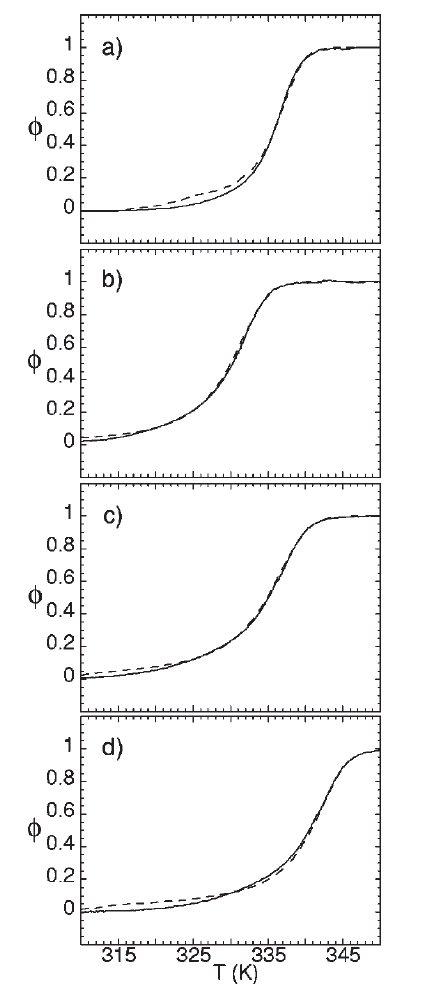
\includegraphics[scale=0.42]{Graphics/DNA/exp.png}
\caption{Experimental melting profiles (full lines) and theoretical results (dashed lines) for three different types of short heterogeneous DNA chains. The temperature is plotted against the average fraction of melted base pairs $\phi$. Subplots (a), (b) and (c) are the melting profiles for the three different DNA chains in a low concentration phosphate buffer solution. Subplot (d) uses the same DNA chain as in (c) but at a much higher concentrations \cite{Campa1998}.}
\label{fig:pbd_exp_test}
\end{figure}
%
Other studies which have investigated the thermodynamics of a heterogeneous PBD model have predicted a multi-step melting behaviour for some long DNA sequences agreeing with experimental observations \cite{Cule1997}. This has been investigated more recently in \cite{Theodorakopoulos2010}. 

The calculations of the eigenvectors and eigenvalues of the PB model go beyond the scope of this review, however. We have outlined the basic principles Peyrard et al. used to apply the transfer integral method. This method will be central to our axial shearing models for both DNA and collagen.

The FJC and WLC models describe the behaviour at a scale where complex polymers are coarse-grained to resemble a singular flexible strand. For DNA these models do not take into account the mesoscopic structure of the two backbones, and complementary base-pairs. As we are interested in DNA shearing and its effects on the base-pairs we will focus our attention on models that include some form of base-pair description. One such model proposed by de Gennes (2001) took a relatively simply approach in studying this behaviour which later became a foundation to other models that we will briefly review \cite{DeGennes2001,Chakrabarti2009,Prakash2011,Mishra2011a}. Collectively, these models showed excellent agreement with experiments when they were compared with results produced by Hatch et al (2008) \cite{Hatch2008}.

To model the force dependence of axial shear pulling de Gennes simplified the structure of DNA to a ladder ignoring the double helical twist, and approximated the backbone, and base-pair potentials to be harmonic with different stiffness constants $Q$ and $R$. By ignoring effects of finite temperature he described the Hamiltonian as a set of one-dimensional displacements for each strand distorted by a force $F$ with the extremities being pulled at either the 3'3' or 5'5' terminals of DNA \cite{DeGennes2001,Hatch2008}, namely
%
\begin{equation}
\label{deGennes_ham}
H=\sum_{-l/2}^{\infty}\frac{Q}{2}\left(u_{n+1}-u_{n}\right)^{2}+\sum_{-\infty}^{l/2}\frac{Q}{2}\left(v_{n+1}-v_{n}\right)^{2}+\sum_{-l/2}^{l/2}\frac{R}{2}\left(u_{n}-v_{n}\right)^{2}
\end{equation}
%
where $u_{n}$ and $v_{n}$ are the axial displacements for each strand with indices $n$ in the range of $-l/2 \leq n \leq l/2$. By defining a critical force for the breakage of a single base-pair to be $R|v_{n}-u_{n}|>f_{c}$ the equilibrium conditions derived from the Hamiltonian allow the overall rupture force $F_{c}$ to be expressed as \cite{DeGennes2001}:
%
%\begin{equation}
%\label{deGennes_eq}
%F_{c}=2 f_{c}\left[\varkappa^{-1}\tanh\left(\frac{\varkappa l}{2}\right)+1\right]
%\end{equation}
%
\begin{equation}
\label{deGennes_eq}
F_{c}=2 f_{c}\varkappa^{-1}\left(1-2\exp^{-\varkappa l}\right)
\end{equation}
%
%
where $\varkappa^{2}=2R/Q$, and $\varkappa^{-1}$ is defined as the number of base-pairs for which the tension is mainly on a single strand; a dimensionless quantity also known as the adjustment length. In this model most of the shear distortion is concentrated near the ends of the ladder structure resulting in larger base-pair axial displacements near $n=\pm l/2$. As we approach the centre of the structure the differential force across the base-pairs tend to zero \cite{DeGennes2001}.
%
\begin{figure}[t]
\centering
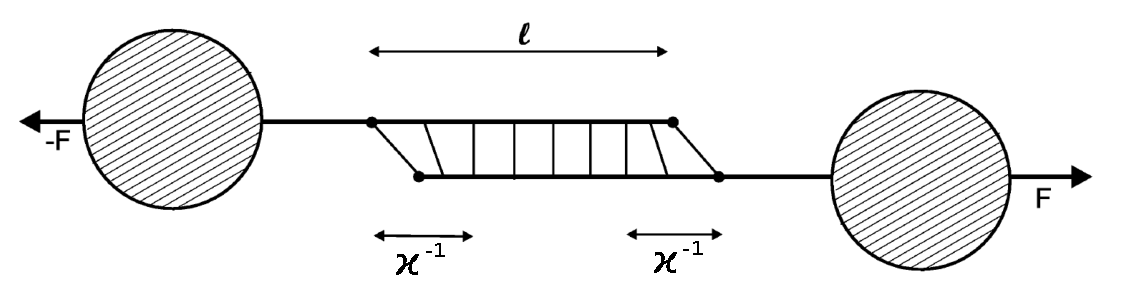
\includegraphics[scale=0.6]{Graphics/DNA/fig1_DeGennes2001.pdf}
\caption{A schematic diagram of the ladder model used by de Gennes. The equal and opposite forces distort the base-pairs over an adjustment length $\varkappa^{-1}$ at both ends of the ladder structure of length $l$. This figure was edited from \cite{DeGennes2001}.}
\label{fig:fig1_DeGennes2001}
\end{figure}
%
Experiments were able to test this model to a high degree of accuracy using magnetic tweezers to probe the shearing force of DNA \cite{Hatch2008}. There is an excellent agreement between experiment and the results predicted by \eqref{deGennes_ham} if we include the effects of a finite number of frayed ends in DNA. Results shown in \figref{fig1_Hatch2008} show that the best fit of de Gennes theory to experiment actually occurs when we assume 7 frayed base-pairs at each end of the ladder structure with $f_{c}=3.9$ pN, $\varkappa^{-1} = 6.8$ bp and stiffness constant ratio of $Q/R = 92.5$ \cite{Hatch2008}. 
%
\begin{figure}[h]
\centering
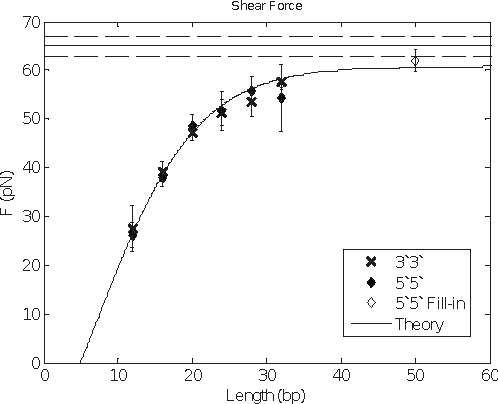
\includegraphics[scale=1]{Graphics/DNA/fig1_Hatch2008.pdf}
\caption{A match between the experimental results of pulling either 3'3' and 5'5' ends produced by Hatch et al with the best fit of \eqref{deGennes_eq}. The horizontal line at $65\pm3$ pN represents the forces characteristic of the over-stretching transitions as measured for the molecule. The upper and lower dashed lines correspond to 110\% and 90\% of the overstretched transition. This figure was taken from in \cite{Hatch2008}.}
\label{fig:fig1_Hatch2008}
\end{figure}
%
Matched by theory, the shear force as a function of number of base-pairs first increases linearly for short DNA lengths, and for larger lengths the critical force saturates below the asymptotic limit of entropic elasticity before the overstretched transition near $65$ pN. Both experiment and theory imply that the mechanical shear stress is localised at the ends of the molecule where the shear force is applied, and that the pulling techniques from 3'3' and 5'5' ends make no difference on the shearing force \cite{Hatch2008}. 

A generalisation of de Gennes model was later studied by Chakrbarti et al (2009) using a semi-microscopic vector model. Based on the same structure as shown in \figref{fig1_DeGennes2001} the model adds further detail to the Hamiltonian by including a stacking interaction term that is expressed as the interactions between nearest neighbours on the same strand, and the interactions between the nearest, and next nearest-neighbour nucleotides of the opposite strand. Keeping the backbone strands harmonic, and using a Lennard-Jones potential for the interaction along the complementary base-pairs the non-linear Hamiltonian can be expressed as \cite{Chakrabarti2009}:
%
\begin{align}
\label{chakrabarti_ham}
H=&\frac{Q}{2}\sum^{L}_{n=1}\left(|\vec{r}_{n+1}-\vec{r}_{n}|-a\right)^{2} +\left(|\vec{s}_{n+1}-\vec{s}_{n}|-a\right)^{2} + \\
&\sum^{L}_{n=1} V_{LJ}\left(|\vec{r}_{n}-\vec{s}_{n}|\right) + V'_{LJ}\left(|\vec{r}_{n+1}-\vec{s}_{n}|\right) + V'_{LJ}\left(|\vec{s}_{n+1}-\vec{r}_{n}|\right)\nonumber
\end{align}
%
where $\vec{r}_{n}$ and $\vec{s}_{n}$ are the position vectors of the $n$th nucleotide along the two backbone strands, $a$ is the equilibrium spacing between the bases along the backbone, and $L$ is the size of the overlap region shown in \figref{fig1_DeGennes2001}. The two additional potential terms labelled $V'_{LJ}$ represent the inter-strand stacking interactions that exist between the base-pairs of DNA. 
%
Though this vector model calculation takes a more complex approach to de Gennes, when coarse-grained, by solving and eliminating all displacements except those that couple directly to the force, \eqref{chakrabarti_ham} reduces to a general non-linear scalar model in terms of displacements projected along the chain. With the base-pair interaction still modelled by a Lennard-Jones potential the Hamiltonian becomes \cite{Chakrabarti2009}
%
\begin{align}
\label{chakrabarti_ham_1}
H=&\frac{Q}{2}\sum^{L}_{n=1}\left(u_{n+1}-u_{n}\right)^{2} +\frac{Q}{2}\sum^{L}_{n=1}\left(v_{n+1}-v_{n}\right)^{2} +\sum^{L}_{n=1}V_{LJ}\left(|u_{n}-v_{n}|\right)\\ &-Fu_{1}+Fv_{L}\nonumber
\end{align}
%
where $u_{n}$ and $v_{n}$ are now the displacements of the top and bottom parts of the ladder structure. Expanding the base-pair potential around the minimum and retaining terms up to the quadratic order we recover a harmonic approximation first studied by de Gennes where the force exceeds a critical value $F_{c} \sim f_{c}N$ for short chains, and $F_{c} \sim 2f_{c}\varkappa^{-1}$ for long chains \cite{Chakrabarti2009}. 

Extending this work further, the statistical mechanics of DNA shearing was later studied at a finite temperature using a Hamiltonian that was similar to the non-linear scalar displacement model of \eqref{chakrabarti_ham_1}. Calculating the shear force $F_{c}$ of DNA as a function of the number of base-pairs, this model developed by Prakash et al. (2011) found that an important factor in getting accurate results was dependent on the choice of values used for the adjustment length and single base-pair breakage force \cite{Prakash2011}. Keeping with the non-linear displacement model where the backbone strands are pulled along the molecular axis by an applied force $F$, the displacements of $i$th nucleotide from its equilibrium position are labelled by $u_{i}$, and $v_{i}$ leading to a Hamiltonian similar to \eqref{chakrabarti_ham}. Transforming the co-ordinate system the displacements of the Hamiltonian can be expressed as two independent components $H_{x}$, and $H_{y}$ in the constant force ensemble \cite{Prakash2011}.
%
\begin{equation}
H=H_{x}+H_{y}
\end{equation}
%
where
%
\begin{equation}
H_{x}=\sum^{N/2-1}_{i=-N/2}\frac{Q}{2}\left(x_{i+1}-x_{i}\right)^{2} - \frac{F}{\sqrt{2}}\left(x_{N/2}-x_{-N/2}\right)
\end{equation}
%
and
%
\begin{equation}
H_{y}=\sum^{N/2-1}_{i=-N/2}\frac{Q}{2}\left(y_{i+1}-y_{i}\right)^{2} + V\left(y_{i}\right) - \frac{F}{\sqrt{2}}\left(y_{N/2}-y_{-N/2}\right)
\end{equation}
%
The base-pair interactions in this model are represented by a potential that encompasses a hardcore repulsion to prevent the compression of base-pairs with respect to its equilibrium, as well as long range interactions. The potential is expressed as
%
\begin{equation}
\label{pe_shikha}
V\left(y_{i}\right)=-\frac{\epsilon}{\left(1+\frac{2y^{2}_{i}}{\sigma^{2}}\right)^{3}}
\end{equation}
% 
where $\epsilon$ is the depth of the potential, and $\sigma$ is the diameter of DNA. In calculating the average positions, $H_{x}$ simplifies $\langle x_{n}\rangle$ to an integral of a Gaussian that can be solved analytically to give 
%
\begin{equation}
\langle x_{n}\rangle = \frac{F}{\sqrt{2}\kappa}n
\end{equation}
%
which agrees with the result found by de Gennes \cite{Prakash2011,DeGennes2001}. The potential term $V\left(y_{i}\right)$ gives the partition function integral of $H_{y}$ a non-Gaussian form and therefore needs to be calculated numerically. Calculating the average displacement quantities Prakash et al. was able to study how the DNA shearing was distributed along the molecule as well as the energies associated with backbone and base-pair stretching. In this constant force model, the shear force needed to separate two strands of DNA was calculated by defining a critical distance $\bar{y}$ needed to rupture a single base-pair. By differentiating the potential \eqref{pe_shikha} with respect to $y$, the critical force for a single base-pair was fitted to be close to the values used by Hatch et al. to fit their experimental data of $f_{c}=4.1$ pN if $y = 2.38$ \AA. The expression for the critical force as derived by Prakash et al. was found to be \cite{Prakash2011}:
%
\begin{equation}
F_{c}=\sqrt{2}\kappa\left(\langle y_{N/2}\rangle - \langle y_{\left(N/2-1\right)}\rangle\right) + 2f_{c}
\end{equation} 
%
When the base-pairs at the ends of that ladder structure $\langle y_{N/2}\rangle$ reach an axial displacement of $\bar{y}$, the point of shearing, the values of $\langle y\rangle$ can be determined. Prakash's results for molecules with 10-60 base-pairs are shown as the dotted curve plotted in \figref{fig6_Prakash2011} and compare well with the experimental results of Hatch et al. 

Alternatively, for a constant extension method the average force is calculated from the amount of work needed to keep the extension of the ladder a distance $y$. From the Hamiltonian the work done by the base-pairs was calculated using the partition function with the constrained displacements imposed using two delta functions for each end, $\delta\left(y_{-N/2}-y\right)\delta\left(y_{N/2}-y\right)$, Prakash et al. described the work done as a function of $y$ by the relations \cite{Prakash2011}:
%
\begin{equation}
\label{shikha_workdone}
W\left(y\right) = \frac{1}{\beta}\left[\ln Z_{N+1}\left(y\right)-\ln Z_{N+1}\right]
\end{equation}
%
where
%
\begin{equation}
Z_{N+1}\left(y\right)=\int \prod^{N/2}_{i=-N/2}dy_{i}\delta\left(y_{-N/2}-y\right)\delta\left(y_{N/2}-y\right)\exp\left(-\beta H_{y}\right)
\end{equation}
%
and 
%
\begin{equation}
Z_{N+1}\left(y\right)=\int \prod^{N/2}_{i=-N/2}dy_{i}\exp\left(-\beta H_{y}\right)
\end{equation}
%
The critical force, $F_{c}$, is now simply the first derivative of \eqref{shikha_workdone} with respect to $y$ taking a value that represents the separation length needed to break a single base-pair $y_{c}$. The dashed curve shown in \figref{fig6_Prakash2011} is plot using the constant extension ensemble with $y$ having a value of $2.0$ \AA. 

Even though both these methods produce slightly different results for molecules of small lengths which later converge for molecules of larger $N$, both these methods agree well with results found by Hatch \cite{Prakash2011}. 
%
\begin{figure}[H]
\centering
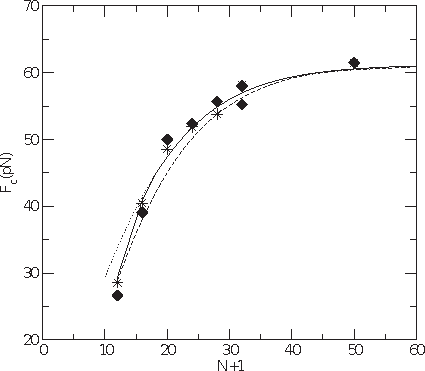
\includegraphics[scale=1.5]{Graphics/DNA/fig6_Prakash2011.pdf}
\caption{Results from the constant force method are shown by the dotted curve, and the constant force method is shown by the dashed curve of the critical force $F_{c}$ as a function of the base-pairs. The experimental results of Hatch et al are shown by diamonds for 5'5' pulling, and stars for 3'3' pulling. This figure was taken from \cite{Prakash2011}.}
\label{fig:fig6_Prakash2011}
\end{figure}
%
Compared with experimental data \cite{Prakash2011,Hatch2008} these models agree well with axial shearing of DNA \figref{fig6_Prakash2011}. For long molecular lengths the models reach an important asymptotic limit giving reasonable fitting parameters to the shearing force of a single base-pair, and stiffness constant ratio between the the backbone and base-pair. These models do not take into account breakage of base-pairs.

\newpage
\section{Collagen}

Collagen is a naturally occurring protein that is a central structural component of multicellular organisms most abundantly found in animals. Forming the major component of the extracellular matrix and connective tissue collagen exist in several distinct types discussed extensively in \cite{Shoulders2009,Fratzl2008,Berg2010,Brinckmann2005}. The collagen subtypes can be found in tissues such as skin, tendon, bone, and cartilage with 80 to 90 percent of the collagen in the human body consisting of types I, II, and III. These collagen molecules pack together to form elongated fibrils of similar structure.  

Reinforcing biological tissues, collagen molecules also pack together to create fibrous polymers that are the major building blocks of all types of load-bearing tissues making the mechanical properties of collagen extremely important \cite{Buehler2006}. In bone and dentin, collagen is combined with mineral to yield very stiff tissues that transmit the force from muscles to bones enabling mammals to physiologically move. In tendon or the cornea, collagen is combined with other organic molecules, such as proteoglycans for different biological functions \cite{Fratzl2008,Bozec2005a,Bozec2007,Ottani2001}.

Due to the limitations in performing mechanical testing on the nanometre and micrometre scale only very recent studies have been initiated to measure the mechanical properties of substructures like collagen fibrils, and tropocollagen \cite{Bozec2005a,Bozec2007,Buehler2006a}.

\subsection{Collagen Structure}

Similar to DNA as well as other proteins, the collagen molecule has a hierarchical structure arising from the interactions of amino acid molecular groups at different levels. Three parallel polypeptide chains, also known as $\alpha$-chains, are made up of repeating amino acid triplets that intertwine in an overall right-handed coil to form the secondary structure of the collagen molecule which is approximately 300 nm long and 1.5 nm wide. This structure is known as a triple helix \cite{Shoulders2009,Fratzl2008,Berg2010,Brinckmann2005,Ramachandran1954,Ottani2001,Bozec2005a,Bozec2007,Buehler2006a}.

\begin{figure}
\centering
\subfloat[]{\label{fig:polypeptide}
\includegraphics[width=0.08\textwidth]{Graphics/Collagen/polypeptide.png}}
\hspace{20 mm}                
\subfloat[]{\label{fig:polypeptide_sapcefilling}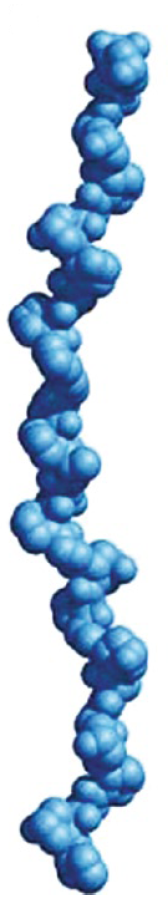
\includegraphics[width=0.09\textwidth]{Graphics/Collagen/polypeptide_spacefilling.png}}
\hspace{20 mm}
\subfloat[]{\label{fig:collagen_molecule}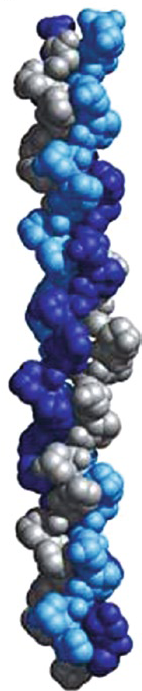
\includegraphics[width=0.1\textwidth]{Graphics/Collagen/tropocollagen.png}}
\caption{Formation of the collagen triple helix from three polypeptide chains. Each polypeptide has a left-handed helical structure as shown in \figref{polypeptide}. A space-filling diagram of the same polypeptide is shown in \figref{polypeptide_sapcefilling}. \figref{collagen_molecule} illustrates three polypeptide chains wrapping around one another with a right-handed twist. (Figure 4.12a, b and c taken from \cite{Nelson2004})}  
\label{fig:polypeptide_to_tropocollagen}
\end{figure}

The amino acids are bound together by peptide bonds which are strong covalent bonds between the carboxyl group and the amino group of each amino acid. Each of the three polypeptides in collagen contains 1000 amino acid residues forming a primary structure that is coiled into a left-handed non-$\alpha$ extended helix. The helix is caused by a steric repulsion of the five-membered heterocycle Pro rings in the hydroxyproline and the proline residues \cite{Shoulders2009,Bhattacharjee2005}. 

\begin{figure}[htp]
\centering 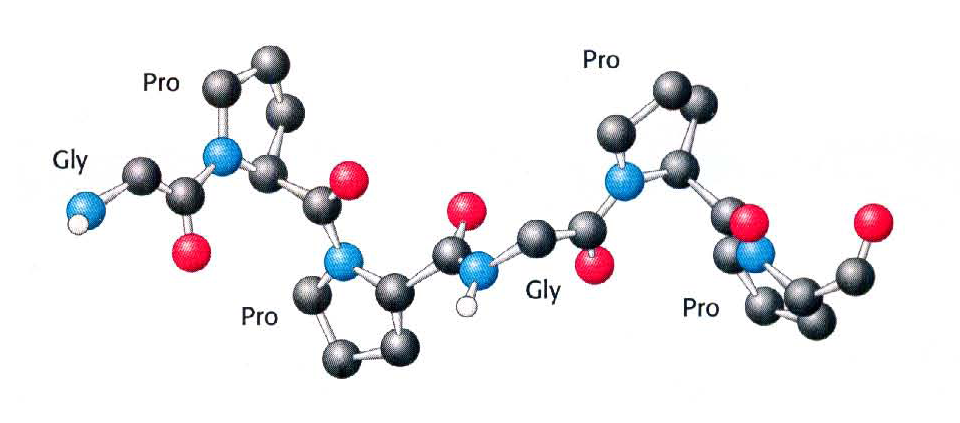
\includegraphics[scale=0.3]{Graphics/Collagen/polypeptide_section_freeman.png}
\caption{A section of a polypeptide showing two amino acid triplets of GlyProHyp covalently bonded by a peptide bond. It also shows the steric repulsion of the heterocyclic rings. (From Fig. 2-39 in \cite{Berg2010})}
\label{fig:col_polyp_sec}
\end{figure}

The tight molecular packing of the three polypeptide chains results in a glycine residue being close to the central core of the triple helix \cite{Shoulders2009,Bhattacharjee2005,Berg2010}. The amino acids in the Xaa and Yaa positions of collagen are often proline and hydroxyproline residues respectively. The compact space near the centre of the triple helix is unable to accommodate any of the larger groups of any amino acid and therefore to maintain stability the large Pro rings are positioned on the outermost part of the triple helix.
  
\begin{figure}
\centering
\subfloat[]{\label{fig:old_td_collagen}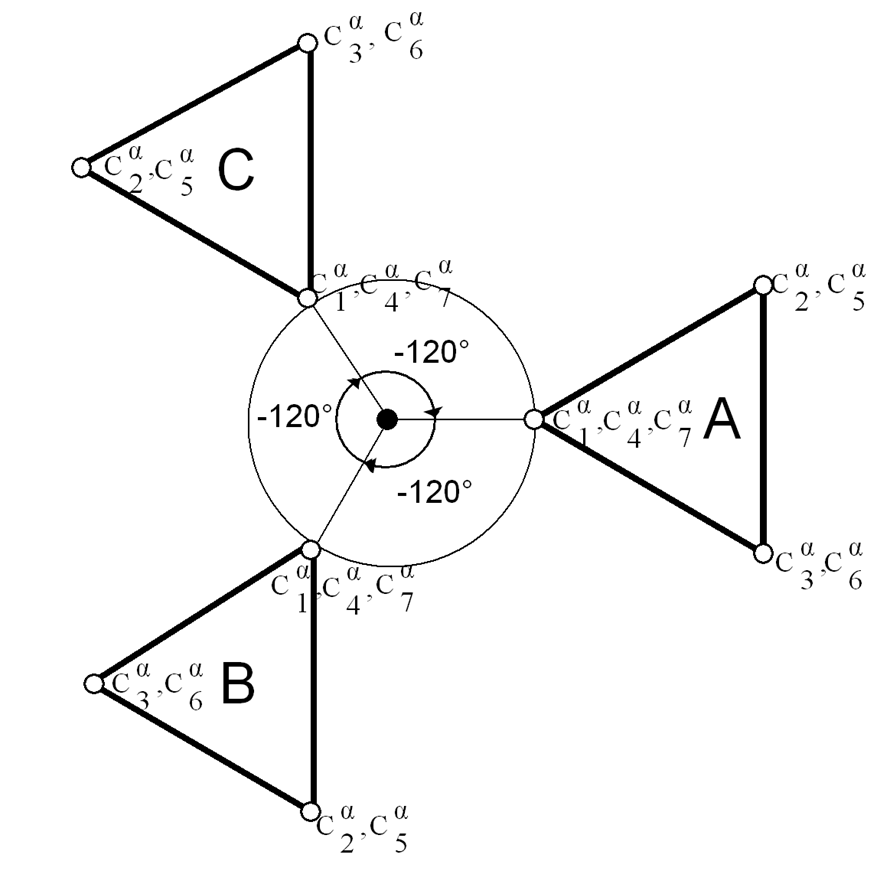
\includegraphics[width=0.275\textwidth]{Graphics/Collagen/old_td.png}}                
\subfloat[]{\label{fig:new_td_collagen}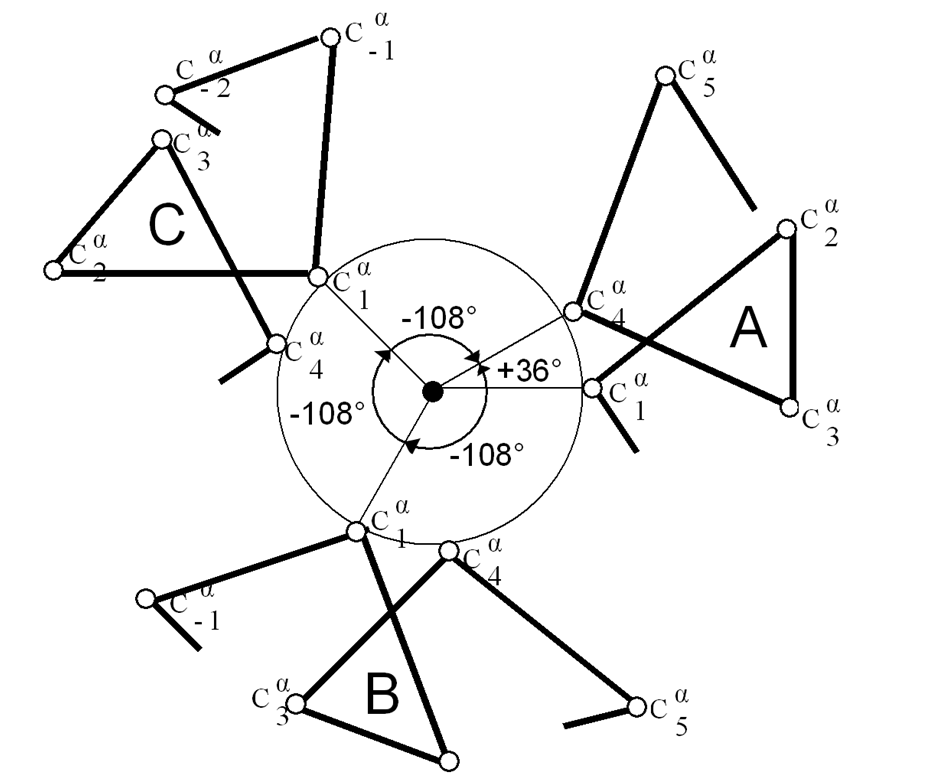
\includegraphics[width=0.3\textwidth]{Graphics/Collagen/new_td.png}}
\subfloat[]{\label{fig:td_freeman}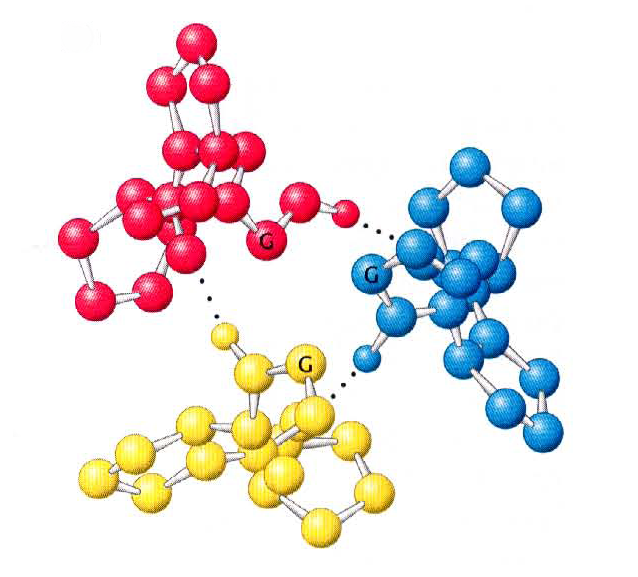
\includegraphics[width=0.3\textwidth]{Graphics/Collagen/td_collagen_freeman.png}}
\caption{A top-down view of the collagen triple helix. The far left \figref{old_td_collagen} was the original structure proposed by Ramachandra \cite{Ramachandran1954} (Figure 1a from \cite{Bhattacharjee2005}). This was later refined by Ramachandra, proposing a coiled structure \cite{Ramachandran1955} in \figref{new_td_collagen} (Figure 1b from \cite{Bhattacharjee2005}). \figref{td_freeman} is a molecular top-down illustration of coiled coil triple helix. } 
\label{fig:top_down_view}
\end{figure}

Ramachandra and Kartha first proposed the first prototype of the right-handed triple helix structure for the collagen molecule in 1954 using X-ray diffraction pictures from different sources \cite{Ramachandran1954}. Their initial structure comprised of three staggered left-handed polypeptides related by a three fold screw symmetry about a common axis, with approximately three residues per turn (\figref{old_td_collagen}) \cite{Ramachandran1954,Bhattacharjee2005}. All peptide bonds were positioned in a trans position and had two hydrogen bonds within each triplet stabilising the triple helix \cite{Ramachandran1954}. This model was later updated to fit observations from X-ray diffraction of stretched collagen fibres which proposed a coiled coil triple helical structure indicating approximately 3.33 residues per turn of the left handed minor helix of each chain \figref{new_td_collagen} \cite{Ramachandran1955}. The major right handed helix had 30 residues per turn. The neighbouring helices in the triple helical assembly are thus related by a twist of $-108^{\circ}$ and rise of $\sim 2.86$\AA \cite{Ramachandran1955,Bhattacharjee2005}. However, this model still caused problems until a refinement by Rich \& Crick showed only one inter-strand hydrogen bond existed per amino acid triplet \figref{schematic_3strand_section} \cite{Rich1955}. 

The collagen triple helix is stabilised by inter-chain hydrogen bond networks. Within each amino acid triplet, one hydrogen bond forms between the amide hydrogen (NH) atom of glycine, a hydrogen bond donor, in one chain and the carbonyl oxygen (C=O) atom of residue X in an adjacent strand, a hydrogen bond acceptor \cite{Ramachandran1954,Rich1955} \figref{schematic_3strand_section}.  Additional stability comes from other weak hydrogen bond systems where the hydrogen of a residue is weakly bonded to the carbonyl oxygen atom of another residue in an adjacent strand, and the two hydrogen atoms of glycine are weakly bonded to the carbonyl oxygen atom of another glycine located in one of the adjacent strands \cite{Perczel2009}.

\begin{figure}[htb]
\centering
\subfloat[]{\label{fig:schematic_3strand_section}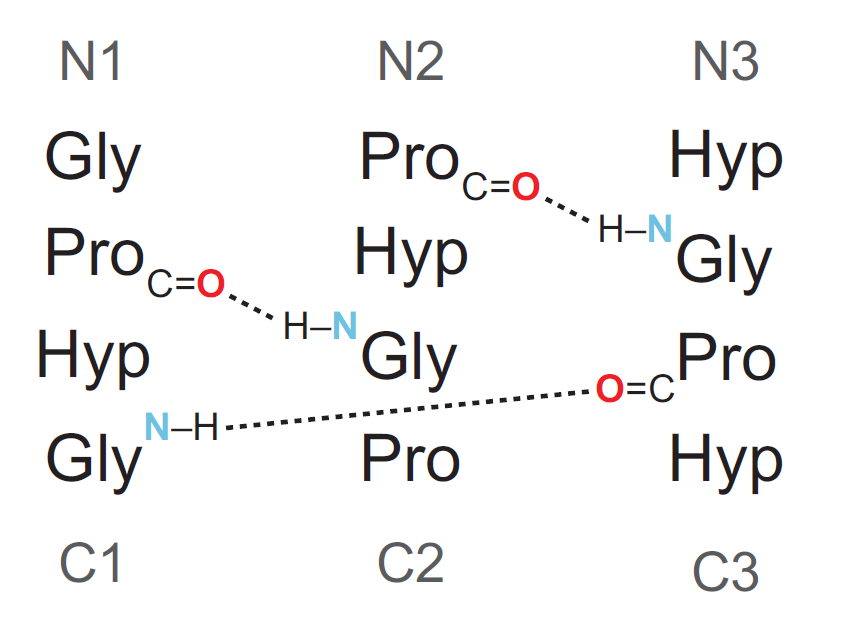
\includegraphics[width=0.3\textwidth]{Graphics/Collagen/shoulders_schematic_polypeptide_3strand.png}}    
\hspace{20mm}            
\subfloat[]{\label{fig:3strand_section}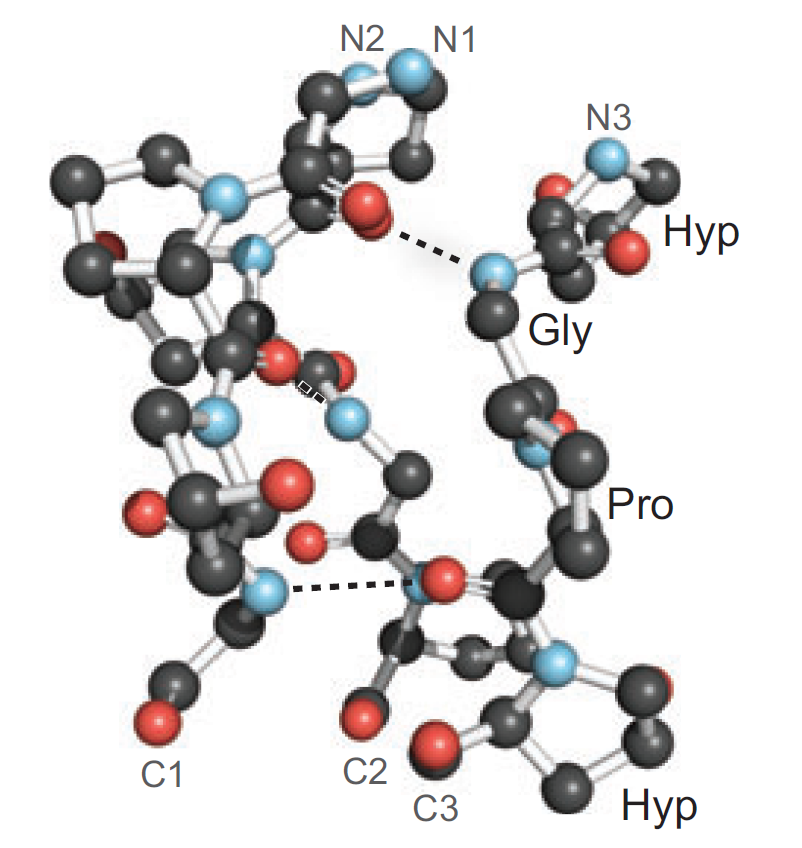
\includegraphics[width=0.3\textwidth]{Graphics/Collagen/shoulders_polypeptide_3strand.png}}
\caption{An illustration showing a segment of the collagen triple helix. A schematic diagram of the segment shows the hydrogen bonds between the amino acid triplet in each polypeptide \figref{schematic_3strand_section} and the ball and stick image shown in \figref{3strand_section} shows a 3D representation of the strong hydrogen bonds, and three polypeptides \cite{Shoulders2009}. (Figures 1c and 1d from \cite{Shoulders2009}.)} 
\label{fig:collagen_segment}
\end{figure}

%\begin{figure}[htp]
%\centering 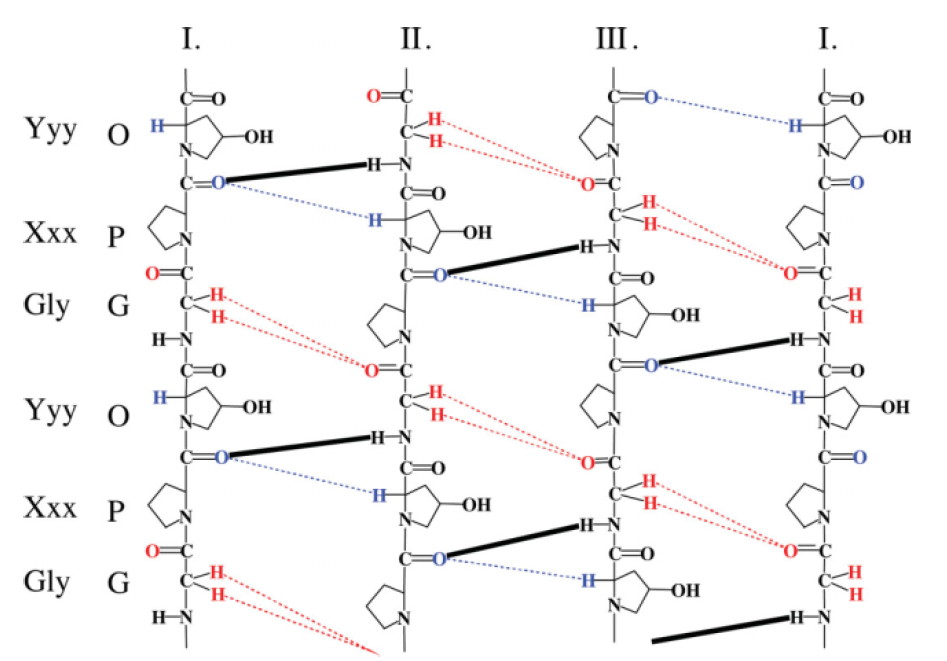
\includegraphics[scale=0.3]{Graphics/Collagen/perczel_collagen_h_network.png}
%\caption{An illustration showing the hydrogen bond networks in tropocollagen. The strong hydrogen bonds are drawn in a strong black lines and the weak hydrogen bonds are depicted by the dashed red and blue lines. The first strand, I, is duplicated at the right to better picture the circular nature of the tropocollagen and its H-bond network \cite{Perczel2009}. (Figure 1 from from \cite{Perczel2009}.)}
%\label{fig:detailed_collagen_h_network}
%\end{figure}

%\begin{figure}[htp]
%\centering 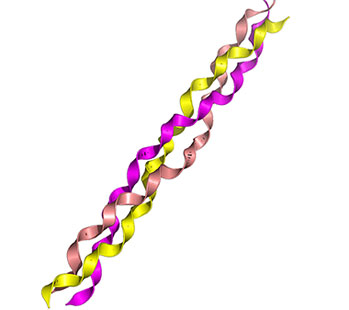
\includegraphics[scale=0.6]{Graphics/Collagen/Collagen1.jpg}
%\caption{}
%\label{fig:col1}
%\end{figure}

%\begin{figure}[htp]
%\centering 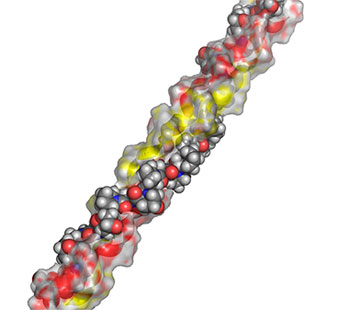
\includegraphics[scale=0.6]{Graphics/Collagen/Collagen2.jpg}
%\caption{}
%\label{fig:col2}
%\end{figure}


\subsection{Collagen Mechanics}

Extensive studies of the mechanical properties of collagen molecules have been made. In single molecule pulling experiments different set-ups have shown that the force-extension behaviour in the entropic elasticity region can be modelled accurately by using the WLC model. At larger forces the increase in tensile strain causes the mechanical behaviour of the molecule to move into the energetic elasticity region where the WLC model fails. We expect to observe the stretching and breaking of hydrogen bonds followed by the deformation of covalent bonds \cite{Buehler2007}. Results from some of the early experiments probing the entropic response of collagen molecules are shown as force-extension curves in \figref{tc_entropic_response}. Investigations by Sun et al. used optical tweezers to stretch human procollagen molecules of type I and II, the precursor form of collagen monomers. The chemical attachment to the beads was achieved by using the abundant amount of disulfide bonds present at the terminal ends of the procollagen molecules. Biotinyated type II procollagen was purified through a desalted column and coated on streptavidin-coated polystyrene beads; one terminal was fixed to a stationary bead on a moving plane while the other terminal was attached to a free bead trapped by optical tweezers \cite{Sun2004}. The molecule was stretched by moving the plane of the fixed bead and measuring the elastic response of the trapped bead using an optical laser \cite{Sun2001}. Fitting their data to the WLC model they found that the collagen monomer had a persistence length of $L_{p} \sim 15 \text{ nm}$ and a contour length of $L \sim 300 \text{ nm}$ \cite{Sun2001,Sun2004}.

\begin{figure}[H]
\centering
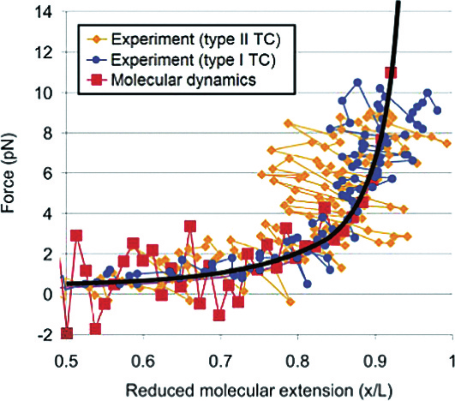
\includegraphics[scale=1]{Graphics/Collagen/Fratzl_2008_fig8p22.pdf}
\caption{A plot of molecular extension of a single collagen molecule in the entropic regime (F \textless 14 pN). The experimental results on type I and type II collagen molecules were reported in \cite{Sun2002,Sun2004} and the MD results were obtained from a study by Buehler et al. using a mesoscale model to predict the force-extension response of a collagen molecule \cite{Buehler2007}. Image was taken from \cite{Fratzl2008}.} 
\label{fig:tc_entropic_response}
\end{figure}

In AFM experiments by Bozec et al. insoluble tropocollagen molecules with cleaved terminals were pulled from a surface without a covalent coupling between the tip and the molecule. This method had no control over the binding processes resulting in cases where multiple molecules were being pulled off the surface, and variations in position where the probe becomes bound to the molecule along its length. Repeat experiments were used to differentiate between single and multiple stretching events. The mechanical properties obtained from this  method of stretching collagen molecules was determined to be only representative of the actual length of the monomer stretched rather than the entire molecule \cite{Bozec2005a}. Shown in \figref{bozec_tc_entropic_response} are the results from these measurements fitted to the WLC model for small extensions. Similar experiments on rat tail tendon by Gutsmann et al. found that the steep increase in force was a result of stretching individual collagen molecules. Their force-extension curves were similar to the ones found by Bozec et al. \cite{Bozec2005a,Gutsmann2004}. They determined the effective contour length of the pulled collagen monomer by fitting their data to the WLC model using a persistence length of $L_{p} \sim 0.4 \text{nm}$.  

Observations made by Bozec et al. did suggest that a proportion of the force-extension curves obtained did feature a discontinuity, thought to be the result of structural changes within the sample, exhibiting a transition to different mechanical behaviour. In data sets where peaks did not exhibit a discontinuity it was found that the WLC model failed at larger extensions \cite{Bozec2005a}. 

\begin{figure}[H]
\centering
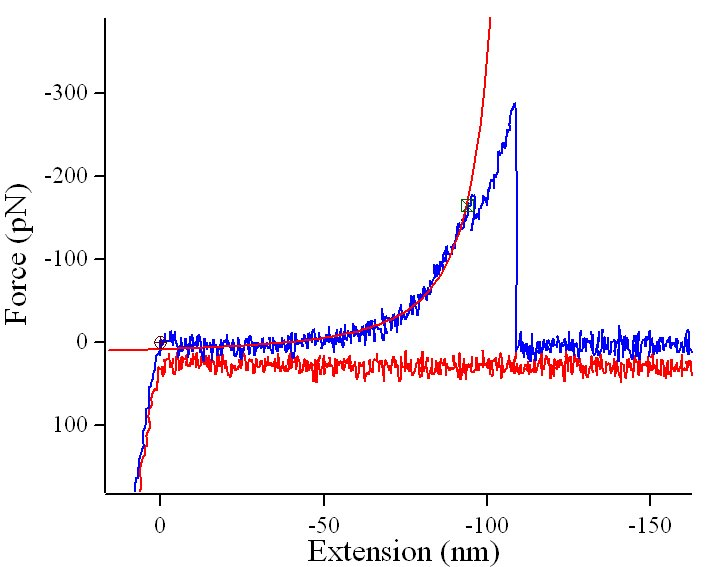
\includegraphics[scale=0.25]{Graphics/Collagen/Bozec_2005.jpg}
\caption{A force extension curve from pulling collagen molecules from a surface using atomic force microscopy. A persistence length of $L_{p} \sim 0.4 \text{ nm}$ was used to fit the WLC model to the data. The discontinuity found in this plot at an extension of approximately 100 nm occurred in 20\% of cases across an entire data set.} 
\label{fig:bozec_tc_entropic_response}
\end{figure}

Recently, molecular dynamic simulations have been used get a better understanding of the nanomechanical properties of tropocollagen molecules \cite{Buehler2007, Lorenzo2005, Buehler2006a, Gautieri2010}. In the full atomistic model calculations by Buehler et al. simulations were run using two types of force field parameters to include the atomistic interactions in proteins: a non-reactive CHARMM force field which provides harmonic and anharmonic terms to describe covalent, van der Waals, and electrostatic interactions, and a reactive ReaxFF force field which includes the dissociation of chemical bonds under deformation \cite{Buehler2006a, Buehler2007}. Fixing one end of the tropocollagen molecule by applying constraints to each of the three carbon atoms, a mechanical load is applied axially using steered molecular dynamics to obtain a force-extension relationship. In these types of MD simulations an external force is applied through a virtual spring with a known stiffness constant to steer the tropocollagen molecule along a path to simulate mechanical stretching also known as steered molecular dynamics (SMD). In both cases Buehler et al. found the results to agree well with experiment for small strains up to 10\% strain but deviated strongly at large strains. The maximum tensile force in the collagen molecule reached , $F \sim 2.35 \times 10^{4} \text{ pN}$ \figref{buehler_cg_model_results}. At $T=300K$ the persistence length was found to be $L_{p} \sim 23.4 \text{ nm}$. Running a simulation for pulling a single polypeptide out of the tropocollagen molecule he found the strength to be $\sim 0.713 \times 10^{4} \text{ pN}$ reaching 3.7\% tensile strain \cite{Buehler2006a}.

\begin{figure}[H]
\centering
\subfloat[]{\label{fig:buehler_cg_model_results}\centering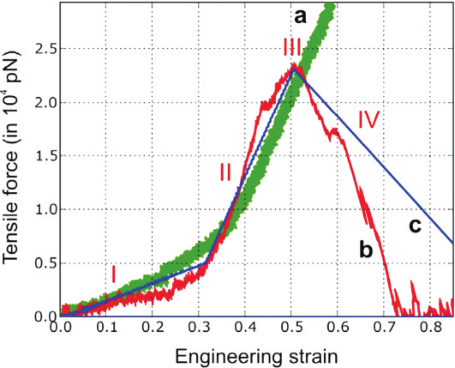
\includegraphics[scale=0.7]{Graphics/Collagen/Fratzl_2008_fig8p2.pdf}}
\hspace{5mm}
\subfloat[]{\label{fig:buehler_cg_model}\centering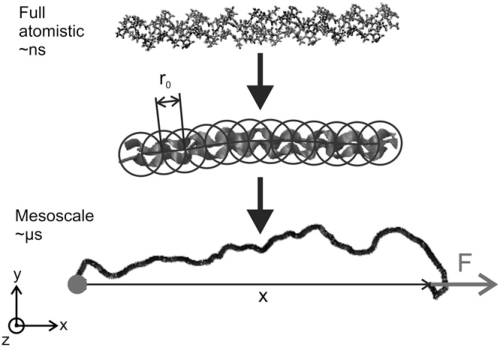
\includegraphics[scale=0.7]{Graphics/Collagen/Buehler_2007_fig4.pdf}}
\caption{The force extension behaviour from the atomistic simulations of a single collagen molecule with $L \sim 8.4\text{ nm}$ are plotted in \figref{buehler_cg_model_results}.  The methods used in these MD simulations had a non-reactive CHARMM force field (a), a reactive ReaxFF force field (b), and a reactive mesoscale model (c) shown in \figref{buehler_cg_model}. The tensile deformation of the molecule starts with the uncoiling of the triple helical structure (I), at larger strains the modulus gradient increases to reflect the stretching of covalent bonds (II). In phase (III) the molecule breaks with a rapid decay of force in phase IV \cite{Buehler2006a, Buehler2007}.} 
\label{fig:buehler_model}
\end{figure}

Taking a coarse-grained approach in the mesoscopic model, Buehler et al. simplified the tropocollagen molecule to a collection of beads. At this level information about the biochemical features within the molecule is lost \figref{buehler_cg_model}. Each bead represents approximately 10 protein atoms having a radius of 7 \AA. Again, one end of the molecule in the simulation is fixed while a force is applied to the other, thus extending the molecule. The MD results shown in \figref{tc_entropic_response} demonstrate a very good agreement with experimental results in the entropic regime. A fit to the WLC model found the persistence length to be $L_{p} \sim 16 \text{ nm}$ where the contour length of the molecule was $L = 301 \text{ nm}$ \cite{Buehler2007}.

In a separate MD study, Gautieri et al. used a coarse-grained MARTINI force-field to model the collagen molecule after making modifications to include parameters that described a hydroxyproline amino acid residue and incorporated the triple helical conformational structure of collagen. All the amino acids are modelled by mapping four non-hydrogen atoms into one bead, and the number of beads used to model a specific residue is decided from the dimensions of the side chain of the amino acid. In determining the force field parameters that describe the triple helix structure of collagen, bond lengths between backbone beads, bonding angles, and dihedral angles were analysed using five collagen-like molecules. These parameters were then used in SMD simulations to obtain a reference force-extension behaviour to determine the elastic stiffness for the potential energy terms in bond stretching, angle deformation, and dihedral deformations \cite{Gautieri2010}. 

\begin{figure}[H]
\centering
\subfloat[]{\label{fig:gautieri_cg_model_comp}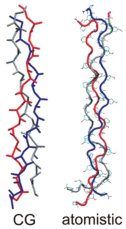
\includegraphics[scale=1.2]{Graphics/Collagen/Gautieri_2010_fig3b.pdf}}
\hspace{10mm}
\subfloat[]{\label{fig:gautieri_cg_model}\raisebox{0.2\height}{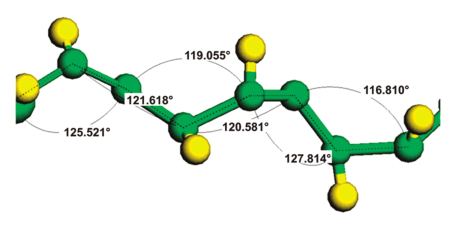
\includegraphics[scale=0.8]{Graphics/Collagen/Gautieri_2010_fig1.pdf}}}
\caption{A comparison between the full atomistic and coarse-grained structures of collagen. Image \figref{gautieri_cg_model} is a detailed view of the coarse grained polypeptides in collagen showing the angles between the backbone beads. The bond lengths between backbone beads, bonding angles, and dihedral angles were computed on the basis of five different collagen molecules. Gautieri et al. obtained a bond reference length $d_{b} = 0.365 \pm 0.07$ nm, a bonding reference angle $\varphi_{a} = 119.2 \pm 8.72^{\circ}$, and a dihedral reference angle $\Psi_{d} =-89.3 \pm 9.76^{\circ}$ \cite{Gautieri2010}.} 
\label{fig:gautieri_MARTINI_model}
\end{figure}

Focusing our attention on the backbone, the spring constant $K_{b}$ was calculated by simulating a single glycine-proline structure and then matching a best fit of the force-extension curve to the full atomistic simulations computed using GROMACS with GROMOS96 43a1 force field parameters. Shown in \figref{gautieri_backbone}, a best fit was found for $K_{b} = 1250 \text{ kJ mol}^{-1} \text{ nm}^{-2}$. Further details of the Extended MARTINI force fields are described comprehensively in \cite{Gautieri2010, Marrink2007, Monticelli2008}. The simulation of a $8 \text{ nm}$ collagen molecule using the coarse-grained model had a stiffness of $1052 \pm 51.23 \text{ pN nm}^{-1}$  up to 15\% strain as shown in \figref{gautieri_results}. In simulating a 300 nm human type I collagen molecule Gautieri et al. obtained a persistence length of $L_{p}=51.5 \pm 6.7 \text{ nm}$.

\begin{figure}[H]
\centering
\centering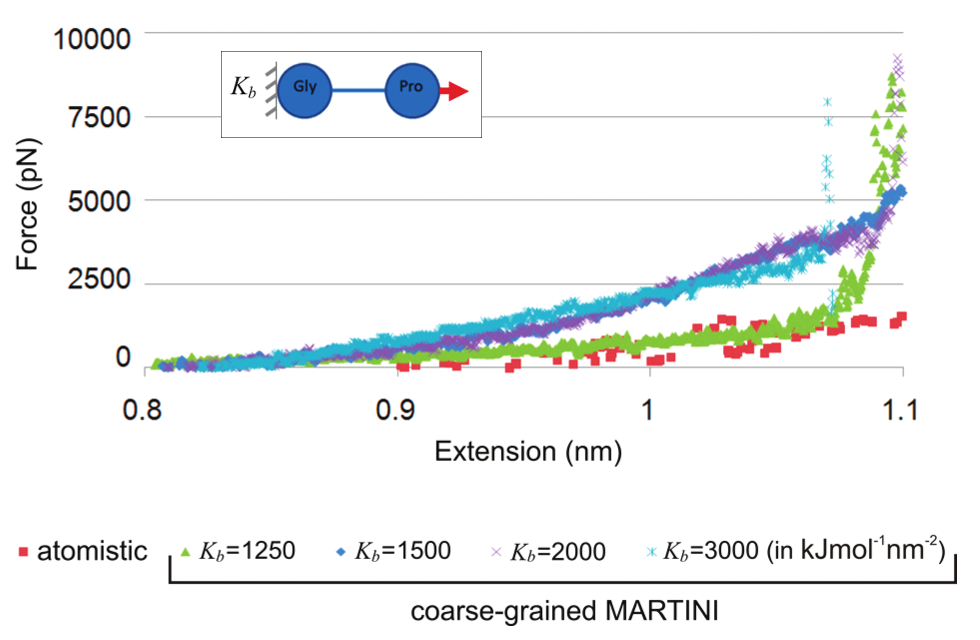
\includegraphics[scale=0.3]{Graphics/Collagen/Gautieri_2010_fig2_combined.png}
\caption{A plot determining the elastic stiffness of the backbone spring constant. The inset diagram is an illustration of the MD simulation studied with the results plotted for various values of $K_{b}$. Data comparison with the atomistic calculations suggest $K_{b} = 1250 \text{ kJ mol}^{-1} \text{ nm}^{-2}$ \cite{Gautieri2010}.} 
\label{fig:gautieri_backbone}
\end{figure}

\begin{figure}[H]
\centering
\label{fig:}\centering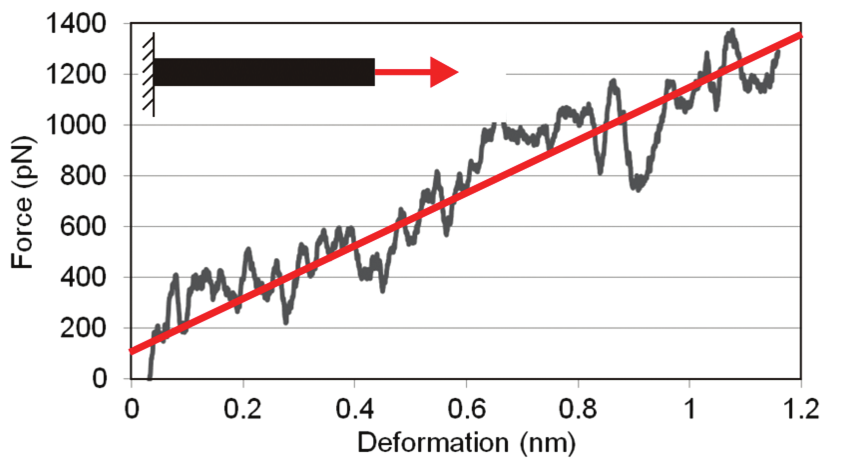
\includegraphics[scale=0.3]{Graphics/Collagen/Gautieri_2010_fig4a.png}
\caption{Force-extension plot of a $8 \text{ nm}$ collagen molecule using the Extended MARTINI force field up to 15\% strain (1.2 nm).} 
\label{fig:gautieri_results}
\end{figure}

Apart from a few pulling experiments of collagen molecules, most of the work described has been focused on the work done by MD simulations giving valuable information on the collagen backbone stiffness. Unfortunately no experimental investigations on the axial shearing of collagen molecules have been found.

\chapter{The Extendable Freely Jointed Chain}

Simple polymer models, excluding the WLC model, are variations of the ideal chain where each link in the chain is described as a uniform rod. To introduce a more realistic behaviour in the FJC we need to add further detail to the description of the polymer on the microscopic scale. We can do this by making each link in the chain extendable, providing extra statistical configurations in space and subsequently altering the entropy and free energy of the system. By considering each segment in the chain to stretch, a modification of the FJC model is obtained, an Extendable Freely Jointed Chain (EFJC) model. In the new model it is assumed that each link within the chain may extend by a small amount contributing to the overall extension of the FJC. By taking each link independently, we can employ a potential energy function to allow for the extensibility. 
We begin by modelling the FJC as analogous to a one dimensional random walk, and then find a relationship between the end position of the random walk and the partition function of an FJC with the same end-to-end separation of the path taken to reach the end position. We then discuss a suitable potential energy function to use for an EFJC, and evaluate the partition function for a FJC and EFJC in one dimension before obtaining them in three dimensions.

\section{Probability Distribution of the Freely Jointed Chain}
\label{sec:probability}

The FJC model can be used to describe the conformations of polymer molecules since the links have the ability to rotate freely around individual nodes and assume a limitless number of orientations \cite{Maarel2008}. Fixing one end of the chain, the other end has a certain probability to lie at any other position in space depending on the position of the previous links. If we set our chain to have $N$ such links each with a length $a$, then one of many possible configurations, and the simplest, is when the chain is fully extended linearly. Here the end-to-end distance of the chain is $l=Na$, which has all the links in the same orientation. The fact that the choice of the orientation of each link is random and that the probabilities of a FJC occupying some configuration in space is finite means that we can treat the FJC model as a random walk through space where the trajectory is the path taken by successive random steps \cite{Maarel2008}. Much like a chain, the length of the link is similar to the step size of the random walk, the number of steps taken in the random walk is equal to the number of links in the FJC, and the probability of a step taken in a random walk is the same as the probability that a link should take a particular configuration in space. The latter does not depend on the previous step or link configuration.

We can determine the probability distribution of end to end distance in the FJC by solving the master equation for a random walk using the multiplicative and additive laws of probability. Starting with,
%
\begin{equation}
P_{N+1}\left(x_{k}\right)=\sum_{k^{'}=-\infty}^{\infty}P_{N}\left(x_{k^{'}}\right)T\left(x_{k}-x_{k^{'}}|x_{k^{'}}\right)\label{MasterEquation}
\end{equation}
%
where $P_{N+1}\left(x_{k}\right)$ is the probability that the walk should end at position $x_{k}$ after step $N+1$ and $T\left(\Delta x|x\right)$ is the transition probability for making a step of size $\Delta x$ given a starting position of $x$. $P_{N+1}\left(x_{k}\right)$ is a sum of probabilities of all the possible previous histories up to this point. For a symmetric random walk in 1-D, where $x_{k}=ka$,
%
\begin{equation}
T\left(x_{k}-x_{k^{'}}|x_{k^{'}}\right)=\frac{1}{2}\left(\delta_{k,k^{'}+1}+\delta_{k,k^{'}-1}\right)
\end{equation}
%
The terms in the brackets represent steps to the right $k=k^{'}+1$ and left $k=k^{'}-1$. Hence, the master equation becomes
%
\begin{equation}
P_{N+1}\left(x_{k}\right)=\frac{1}{2}P_{N}\left(x_{k-1}\right)+\frac{1}{2}P_{N}\left(x_{k+1}\right)
\end{equation}
%
which when solved gives the result, for $|k|\leq N$, and even $(N-k)$ ~\cite{Reif1965}:
%
\begin{equation}
P_{N}\left(x_{k}\right)=\frac{1}{2^{N}}\frac{N!}{\left(\frac{N-k}{2}\right)!\left(\frac{N+k}{2}\right)!}\label{SolvedMasterEquation}
\end{equation}
%
A plot of this distribution in \figref{ProbabilityDistributionN24610} shows that the probability is greatest for $x_{k}=0$. This is true for all $N$. For larger values of $N$ the random walk is able to follow more trajectories reaching higher values of $x_{k}$, hence we see a broader probability distribution for $N=10$ when compared to $N=2$. 

Taking the sum over all possible configurations we can express the probability density function of walk displacement $R$ as
%
\begin{equation}\label{MasterEqFJC}
P_{N}\left(R\right)=\sum_{k}P_{N}\left(x_{k}\right)\delta\left(x_{k}-R\right)
\end{equation}
%
where the delta function specifies integer values for the continuous walk displacement $R$. With the expression for $P_{N}\left(x_{k}\right)$ being a set of binomial coefficients we can represent \eqref{MasterEqFJC} as
%
\begin{align}
P_{N}\left(R\right)&=\frac{1}{2^{N}}\sum_{k=-N}^{N}\binom{N}{\frac{N+k}{2}}\delta\left(x_{k}-R\right)\\
&=\frac{1}{2^{N}}\sum_{K=0}^{N}\binom{N}{K}\delta\left(x_{2K-N}-R\right)\label{pdist}
\end{align}
%
where $K=\frac{N+k}{2}$ \cite{Reif1965}. The probability that the walk should end with a displacement in $R\rightarrow R+dR$ in the continuous limit would then be $\int P_{N}\left(R\right)dR$, but since $R$ is an integer the probability of obtaining the result in $R_{1} \leq R \leq R_{2}$ is $\int^{R_{2}}_{R_{1}} P_{N}\left(R\right)dR$.

When $x_{k}=Na$ the FJC is linear; This being in only one possible configuration we find it has the least probability of being in this state. This is demonstrated in \figref{ProbabilityDistributionN24610} and \figref{ProbabilityDistributionN2}. Treating the FJC now in statistical mechanics we can expect the partition function of the system with end-to-end separation $R$ to be the greatest when $R=0$. The end-to-end polymer length $R$ is analogous to the displacement $x_{k}$ in the random walk. In relation to higher values of $N$ we can expect the distribution to broaden.

\begin{figure}[H]
\centering 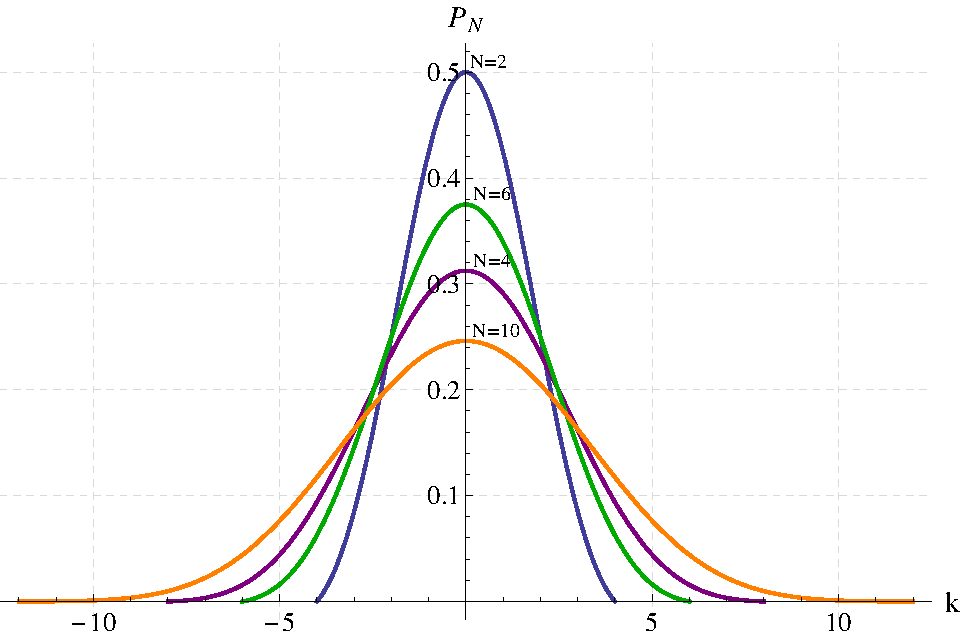
\includegraphics[scale=0.6]{Graphics/ExpectedProbabilityDistribution.pdf}
\caption{A plot showing an envelope of the expected probability distribution over position $x_{k}$
for $N=2,4,6,10$. The probability distributions are the sum of contributions over
all paths.}
\label{fig:ProbabilityDistributionN24610} 
\end{figure}

\begin{figure}[H]
\centering 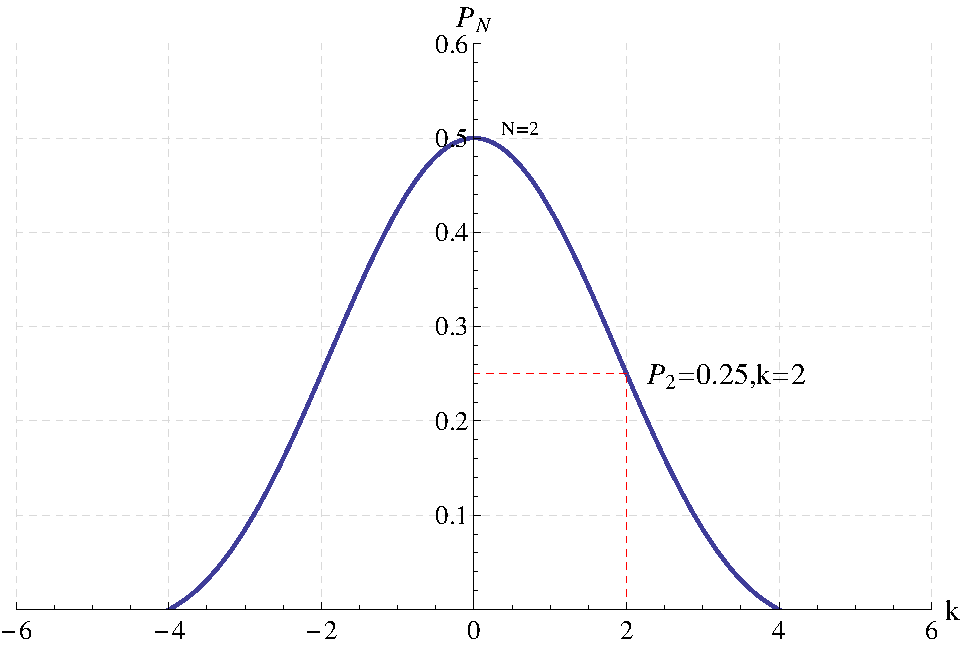
\includegraphics[scale=0.6]{Graphics/ExpectedProbabilityDistributionN2.pdf}
\caption{A plot showing an envelope of the expected probability distribution of displacement $x_{k}$ for $N=2$.
The dashed lines indicate that the end position is twice as likely to be at the origin, $x_{k}=0$ than to be at either $x_{k}=2a$ or $x_{k}=-2a$.}
\label{fig:ProbabilityDistributionN2} 
\end{figure}


\section{Construction of the Partition Function Integral}

In constructing our partition function for an EFJC we will consider a system consisting of $N+1$ particles each of which interacts with its neighbouring particles. The partition function is an integral over phase-space of the exponential of the system's Hamiltonian. The integral represents the sum over all configurations for a $N$-particle system. The Hamiltonian will later allow us to include our desired potential. We work initially in one dimension. The partition function in a system with $N$ links is 
%
\begin{equation}
\mathcal{Z}=\frac{1}{h^{N}}\int\prod_{i=1}^{N}dq_{i}dp_{i}\,\exp\left(-H\left(p_{i},q_{i}\right)/kT\right)\label{ClassicalPartitionFunction}
\end{equation}
%
where $h$ is Planck's constant, $q_{i}$ is the phase space co-ordinate of the $i^{th}$ particle, $p_{i}$ is its momentum, $H\left(p_{i},q_{i}\right)$ is the Hamiltonian, $k$ is the Boltzmann constant, and $T$ is the absolute temperature. The zeroth particle is held static at the origin.

The Hamiltonian, which is a function of both position and momentum, represents the total energy of the system. It is the sum of the kinetic energy and the potential energy of all the constituents,
%
\begin{equation}
\widehat{H}\left(p_{i},q_{i}\right)=\sum_{i=1}^{N}\left(\frac{p_{i}^{2}}{2m}+\Phi\left(q_{i},q_{i-1}\right)\right)\label{Hamiltonian}
\end{equation}
%
where $m$ is the mass of each particle and $\Phi\left(q_{i},q_{i-1}\right)$ is the potential controlling the length of each link. Because the position and momentum parameters are independent in the Hamiltonian it allows us to fully separate the spatial and momentum integrations of the partition function \eqref{ClassicalPartitionFunction}.
%
\begin{align}
\mathcal{Z} & =\frac{1}{h^{N}}\int\prod_{i=1}^{N}dp_{i}\,\exp\left(-\frac{p_{i}^{2}}{2mkT}\right)\,\int\prod_{i=1}^{N}dq_{i}\,\exp\left(-\frac{\sum_{i=1}^{N}\Phi\left(q_{i},q_{i-1}\right)}{kT}\right)\nonumber\\
 & =\frac{1}{h^{N}}Z_{p}Z_{q}\label{SeparableClassicalPartitionFunction}
\end{align}
%
The momentum partition function in \eqref{SeparableClassicalPartitionFunction} is simply a Gaussian integral raised to the power of $N$. This allows us to integrate over the momentum for all the individual links in the chain. It can be simplified to a constant leaving the position partition function integral to be evaluated. 
%
\begin{equation}
Z_{p}=\left(2\pi mkT\right)^{\frac{N}{2}}\label{MomentumPartitionFunction}
\end{equation}
%
The breakdown of the dimensionless partition function gives the position integral $Z_{q}$ a dimension of length to the power of $N$. To simplify the position integral in \eqref{SeparableClassicalPartitionFunction} the potential $\Phi\left(q_{i},q_{i-1}\right)$ needs to be written in terms of a set of variables, $q_{i,i-1}=\left(q_{i}-q_{i-1}\right)$. The Jacobian for this change in variables is unity. A Fourier transform representation of the Dirac delta function is then inserted into the partition function to impose the following constraint. We consider the case where the end-to-end polymer length is equal to $R$, where $R=q_{N}-q_{0}$. We write 
%
\begin{equation}
Z_{q}=\int^{\infty}_{-\infty} \, dR\, Z_{q}\left(R\right)
\end{equation}
%
with
%
\begin{equation}
Z_{q}\left(R\right) = \int\prod_{i=1}^{N}dq_{i} \delta\left(q_{N}-q_{0}-R\right) \exp\left(-\frac{\sum_{i=1}^{N}\Phi\left(q_{i}-q_{i-1} \right)}{kT}\right)
\end{equation}
%
and employ
%
\begin{align}
\delta\left(q_{N}-q_{0}-R\right) & =\delta\left(\sum_{i=1}^{N}q_{i,i-1}-R\right)\nonumber\\
&=\frac{1}{2\pi}\int_{-\infty}^{\infty}d\omega\,\exp\left[i\omega\left(\sum_{i=1}^{N}q_{i,i-1}-R\right)\right]\label{BoundaryCondition}
\end{align}
%
Inserting \eqref{BoundaryCondition} into $Z_{q}\left(R\right)$, we get
%
\begin{align}
Z_{q}\left(R\right) & =\int_{-\infty}^{\infty}\prod_{i=1}^{N}\left[dq_{i,i-1}\exp\left(-\frac{\Phi\left(q_{i,i-1}\right)}{kT}\right)\right]\frac{1}{2\pi}\int_{-\infty}^{\infty}d\omega\,\exp\left[i\omega\left(\sum_{i=1}^{N}q_{i,i-1}-R\right)\right]\nonumber\\
 & =\frac{1}{2\pi}\int_{-\infty}^{\infty}d\omega\,\exp\left(-i\omega R\right)\left[\int_{-\infty}^{\infty}dq_{i,i-1}\,\exp\left(-\frac{\Phi\left(q_{i,i-1}\right)}{kT}\right)\,\exp\left(i\omega q_{i,i-1}\right)\right]^{N}\label{FourierTransformPartitionFunction}
\end{align}
%
Using a suitable potential we can solve \eqref{FourierTransformPartitionFunction} to find the partition function. In the next section we will discuss potential energy functions to describe a FJC and an EFJC.

\subsection{Quadratic Potential}

For an illustration of how one might solve the partition function using the Fourier transform partition function, \eqref{FourierTransformPartitionFunction}, we will begin by fixing the configuration of the EFJC to be linear, and then allow each link to extend harmonically. The focus on a linear configuration takes the model away from a theory of polymers to a theory of an elastic rod. Considering only the 1-D case along the $x$-axis the harmonic
potential is
%
\begin{equation}
\Phi\left(x\right)=\frac{1}{2}\alpha\left(x-a\right)^{2}\label{ElasticPotential}
\end{equation}
%
where $a$ corresponds to the length of each link in the absence of a load, and $\alpha$ is the spring constant. Combining the elastic
potential with \eqref{FourierTransformPartitionFunction} gives
%
\begin{equation}
Z_{q}^{rod}\left(R\right)=\frac{1}{2\pi}\int_{-\infty}^{\infty}d\omega\, \exp\left(-i\omega R\right)\left[\int_{-\infty}^{\infty}dx\, \exp\left(-\frac{\alpha\left(x-a\right)^{2}}{2kT}\right)\, \exp\left(i\omega x\right)\right]^{N}
\end{equation}
%
which when evaluated gives an expression
%
\begin{equation}
Z_{q}\left(R\right)=\left(\frac{2\alpha\pi}{NkT}\right)^{\frac{1}{2}}\left(\frac{2kT\pi}{\alpha}\right)^{\frac{N}{2}}\exp\left(-\frac{\alpha\left(R-aN\right)^{2}}{2kTN}\right)\label{Z_ElasticPotential}
\end{equation}
%
The case described by \eqref{Z_ElasticPotential} corresponds to one configuration of the EFJC with $R=Na$ .
%Since the rod has links that move independently we would expect the maximum partition function value to be at $R=Na$ as there are more configurations the rod can take for end position to be at $R=Na$. The case described by \eqref{Z_ElasticPotential} only takes into account one configuration of the EFJC. 
The results from \figref{GraphElasticPotential} show that \eqref{Z_ElasticPotential} for N=4 describes a Gaussian distribution peaking at $R=4a$. This is the unstretched length of the rod. Irrespective of the many random configurations each link can take within the EFJC, all the links described by this partition function follow the same direction to make the chain comparable to a rod of length $Na$. 

\begin{figure}[htp]
\centering 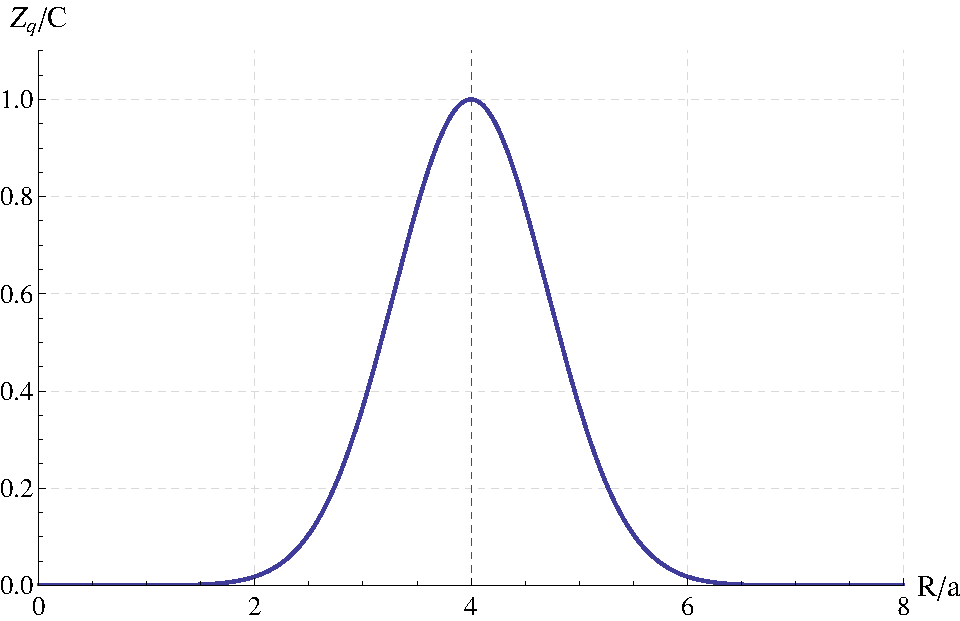
\includegraphics[scale=0.6]{Graphics/zElasticPotential.pdf} 
\caption{A plot showing the value of $Z_{q}/C$ as a function of $R$ using
an harmonic potential for $N=4$. The constant $C$ is a scaling factor and $\alpha/2kTN$ is set to unity.}
\label{fig:GraphElasticPotential} 
\end{figure}

\subsection{Double Potential}

We will begin by looking at how we can create a suitable potential to describe the behaviour of the links that make up the FJC. In modelling each link we will imagine that one end of the link is fixed while the other end is free to lie in any direction characterised by a potential. By subsequently using this method for $N$ links we create an FJC. For example, if the length of a link is $a$, and consider one end of the link to be fixed at a point $\beta$ on the $x$-axis, the other end would be positioned at either $\beta+a$ or $\beta-a$. We can allow each link to have this spatial freedom by setting up a potential, $\Phi\left(x\right)$, that is infinite everywhere except at $a$ and $-a$. The exponential of the potential as seen in \eqref{FourierTransformPartitionFunction}, should correspond to two Dirac delta weighting functions with zero weight everywhere except at $a$ and $-a$. The link cannot be extended further than its unperturbed length, $a$. This potential would describe a non-extendable FJC in one dimension. The potential for the FJC is inserted such that
%
\begin{equation}\label{tophatdeltapotential}
\exp\left(-\frac{\Phi\left(q_{i,i-1}\right)}{kT} \right) = \frac{A}{2}\left( \delta\left(q_{i,i-1}-a\right) + \delta\left(q_{i,i-1}+a\right)  \right)
\end{equation}
%
where $A$ is a constant with dimensions of length. 
%
\begin{figure}[H]
\centering 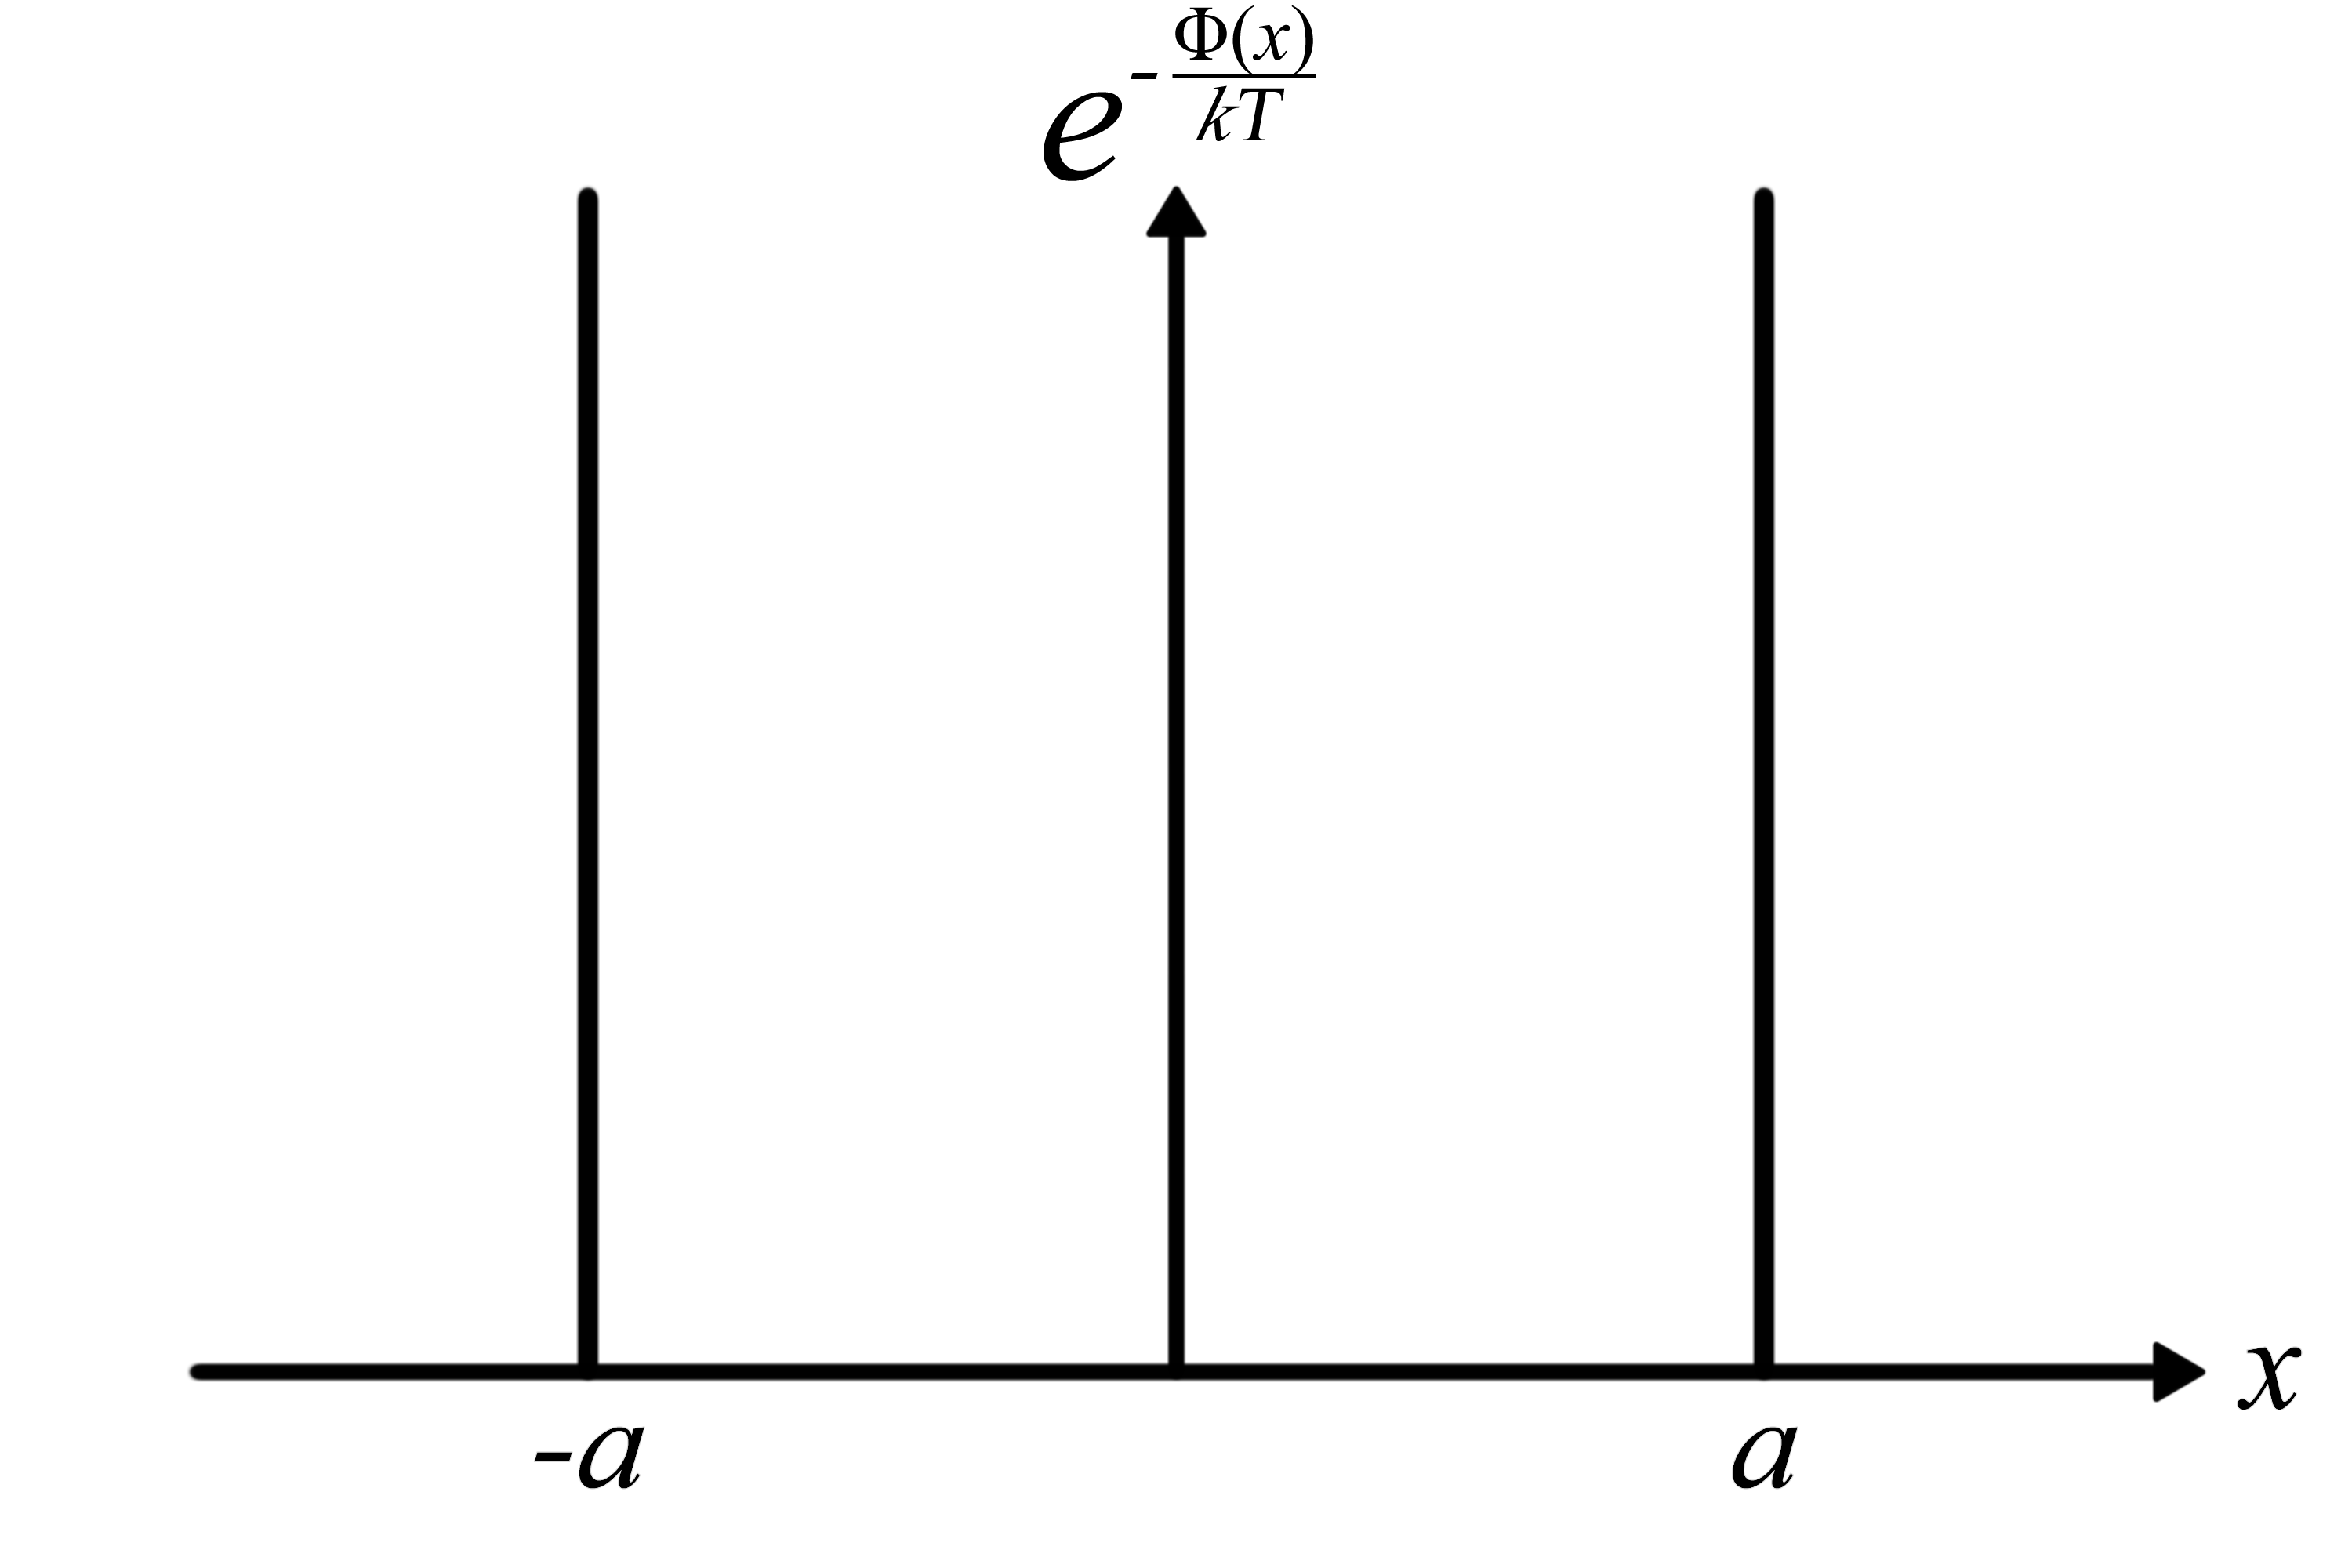
\includegraphics[scale=0.6]{Graphics/DoubleDeltaFunction.png} 
\caption{A plot of the double delta function weighting function where the value of $\exp\left(-\frac{\Phi\left(x\right)}{kT}\right)$ is infinite at $\pm a$.}
\label{fig:DoubleDeltaFunctionPotential} 
\end{figure}
%
The partition function is then
%
\begin{equation}\label{deltapf}
Z_{q}\left(R\right) = \int\prod^{N}_{i=1} dq_{i,i-1}A^{N}\delta\left(\sum_{i=1}^{N}q_{i,i-1} - R\right)\prod_{i=1}^{N}\left( \frac{1}{2}\left( \delta\left(q_{i,i-1}-a \right) + \delta\left(q_{i,i-1}+a \right)   \right)\right)
\end{equation}
%
This is intuitively proportional to a sum over paths, constrained such that the total displacement is $R$ through the first delta function in \eqref{deltapf}. Each step is $\pm a$ imposed by each of the second set of delta functions. It is therefore the sum of all possible outcomes of the symmetric random walk with given $R$. This establishes the analogy between $Z_{q}\left(R\right)$ and $P_{N}\left(R\right)$ derived in \ref{sec:probability}. The normalisation of the probability distribution for $R$ requires that
%
\begin{equation}
P_{N}\left(R \right)= \frac{Z_{q}\left(R\right)}{\int\,dR Z_{q}\left(R\right)}
\end{equation}
%
The transition probability of the analogous random walk is 
%
\begin{equation}
T\left(q_{i,i-1}\right)=  \frac{1}{2}\left( \delta\left(q_{i,i-1}-a \right)+ \delta\left(q_{i,i-1}+a \right)\right)  
\end{equation}
%
This is normalised such that 
%
\begin{equation}
\int^{\infty}_{-\infty}T\left(q_{i,i-1}\right)dq_{i,i-1} = 1
\end{equation}
%
In order to pursue the analogy to a random walk, we need to employ a weighting function such that the transition probability in the analogous random walk is
%
\begin{equation}
T\left(q_{i,i-1}\right)=\frac{\exp \left(-\frac{\Phi\left(q_{i,i-1}\right)}{kT}\right)}{\int^{\infty}_{-\infty} \exp \left( -\frac{\Phi\left(q_{i,i-1}\right)}{kT} \right) dq_{i,i-1}}
\end{equation}
%
which is correctly normalised.


\subsection{Evaluating $\boldsymbol{{Z_{q}\left(R\right)}}$ for the non-extendable Freely Jointed Chain}

Following on from \eqref{deltapf}, where the exponential term is replaced by two delta weighted functions, the partition function
becomes
%
\begin{equation}
Z_{q}\left(R\right)=\frac{A^{N}}{2\pi}\int_{-\infty}^{\infty}d\omega\, e^{-i\omega R}\left[\frac{1}{2}\int_{-\infty}^{\infty}dx\,\left\{ \delta\left(x-a\right)+\delta\left(x+a\right)\right\} e^{i\omega x}\right]^{N}
\end{equation}
%
Taking the terms that correspond to the Fourier transform of the weighting function as $\kappa\left(\omega\right)$, and using the sifting property of the Dirac delta function we get the following \cite{Riley2002},
%
\begin{equation}
Z_{q}\left(R\right)=\frac{A^{N}}{2\pi}\int_{-\infty}^{\infty}d\,\omega e^{-i\omega R}\left[\kappa\left(\omega\right)\right]^{N}
\end{equation}
%
where
%
\begin{align}
\kappa\left(\omega\right)&=\frac{1}{2}\int_{-\infty}^{\infty}\delta\left(x-a\right)e^{i\omega x}dx+\frac{1}{2}\int_{-\infty}^{\infty}\delta\left(x+a\right)e^{i\omega x}dx \\
&=\frac{e^{i\omega a}+e^{-i\omega a}}{2}\\
&=\cos \omega a
\end{align}
%
The partition function then becomes
%
\begin{equation}
Z_{q}\left(R\right)=\frac{A^{N}}{2\pi}\int_{-\infty}^{\infty}d\omega\, e^{-i\omega R}\cos^{N}\omega a
\end{equation}
%
The cos term which is raised to the $N^{th}$ power can be expressed as a sum of exponentials using the binomial theorem,
%
\begin{equation}
\cos^{N}x=\frac{1}{2^{N}}\sum_{k=0}^{N}\binom{N}{k}e^{ix(N-2k)}\label{Cos_Series}
\end{equation}
%
for all integer $k$. Combining this and the general integral representation of the Dirac delta function \cite{Riley2002}
%
\begin{equation}
\delta(x)=\frac{1}{2\pi}\int_{-\infty}^{\infty}e^{-ixt}\, dt
\end{equation}
%
we get
%
\begin{align}
Z_{q}\left(R\right) & =\frac{A^{N}}{2^{N+1}\pi}\sum_{k=0}^{N}\binom{N}{k}\int_{-\infty}^{\infty}e^{-i\omega\left(R+2k-N\right)}\, d\omega\\
 & =\frac{A^{N}}{2^{N+1}\pi}\sum_{k=0}^{N}\binom{N}{k}\delta\left(R+2k-N\right)\label{pfSolved1D_1}\end{align}
%
Here we obtain the partition function for a FJC in one dimension. Evaluating the integral of \eqref{pfSolved1D_1} with respect to $R$ we can show that
%
\begin{equation}
\int Z_{q}\left(R\right)\,dR = \frac{A^{N}}{2^{N+1}\pi}\sum_{k=0}^{N}\binom{N}{k}= \frac{A^{N}}{2\pi} 
\end{equation}
%
and hence
%
\begin{equation}
P_{N}\left(R\right) = \frac{Z_{q}\left(R\right)}{\int Z_{q}\left(R\right)\,dR} = \frac{1}{2^{N}}\sum^{N}_{k=0}\binom{N}{k}\delta(R+2k-N)
\end{equation}
%
as derived earlier in \eqref{pdist}. Taking this further, the partition function for the EFJC will next be calculated using an appropriate weighting function.

\section{Extendable Freely Jointed Chain Model in One Dimension}

\subsection{Potential for an Extendable Freely Jointed Chain}

To make the FJC extendable we replace the double delta function weighting factors with two top-hat functions of finite width $p$. This corresponds to a pair of infinite square wells and since they have a finite width $p$, it allows each link is able to extend and contract by a length $\frac{p}{2}$ without a cost in energy. The normalised transition probability for the random walk analogous to the EFJC would be $T\left(q_{i},q_{i-1}\right)$ such that
%
\begin{equation}
\int^{\infty}_{-\infty}T\left(q_{i,i-1}\right)dq_{i,i-1}=\frac{1}{2p}\left[\int_{-a-\frac{p}{2}}^{-a+\frac{p}{2}}\,dq_{i,i-1} + \int_{a-\frac{p}{2}}^{a+\frac{p}{2}}\,dq_{i,i-1}\right]=1
\end{equation} 
%
The effect of taking the limit of $p\rightarrow0$ whilst preserving the normalisation makes the height of each weighting function infinitely large such that they become delta functions. Analytically, we can show that our top-hat weighting functions become proportional to delta functions in the limit of $p\rightarrow0$ by using a combination of Heaviside functions to express an integral over finite limits as an integral over all space.
%
\begin{equation}
H(x)=\int_{-\infty}^{x}\delta(t)dt\label{HeavisideFunction}
\end{equation}
%
Starting with the top-hat weighting functions in one dimension we can express the weight of the potential as two separate integrals where the width of weighting function $\varsigma(x)$ is contained in the integral limits.
%
\begin{equation}
\int_{a-\frac{p}{2}}^{a+\frac{p}{2}}\varsigma(x)\, dx+\int_{-a-\frac{p}{2}}^{-a+\frac{p}{2}}\varsigma(x)\, dx\label{IntegralOfWeight}
\end{equation}
%
Representing a top-hat weighting function with two Heaviside step functions we have \cite{Bronshtein2007},
%
\begin{equation}
\sqcap\left(x;p\right)\equiv H\left(x+\frac{p}{2}\right)-H\left(x-\frac{p}{2}\right)\label{Top-Hat}
\end{equation}
%
Where $x$ would be the centre position of the top-hat function. The weighting factor in the integrand, and implicitly the potential $\Phi$, will be written 
%
\begin{equation}\label{tophatpotential}
\exp\left(-\frac{\Phi\left(q_{i,i-1}\right)}{kT}\right)= \frac{A}{2p}\left(\sqcap\left(x-a;p\right)+\sqcap\left(x+a;p\right)\right)
\end{equation}
%
Where $A$ again has dimensions of length, and will turn out to be analogous to the $A$ in \eqref{tophatdeltapotential}. Using \eqref{Top-Hat} each integral in \eqref{IntegralOfWeight} can now be expressed as an integral over all space,
%
\begin{align}
\int_{a-\frac{p}{2}}^{a+\frac{p}{2}}\varsigma(x)\, dx & =\int_{-\infty}^{\infty}\sqcap\left(x-a;p\right)\varsigma(x)\, dx\\
\int_{-a-\frac{p}{2}}^{-a+\frac{p}{2}}\varsigma(x)\, dx & =\int_{-\infty}^{\infty}\sqcap\left(x+a;p\right)\varsigma(x)\, dx
\end{align}
%
The positions $a$ and $-a$ correspond to the positions of the top-hat potentials as shown in \figref{DoubleTophatPotential}. Since the value of $p$ is small and finite we can use the mean value theorem for integration to express each integral as,
%
\begin{align}
\int_{-\infty}^{\infty}\frac{1}{p}\sqcap\left(x-a;p\right)\varsigma(x)\, dx & =\varsigma\left(\tau\right)\\
\int_{-\infty}^{\infty}\frac{1}{p}\sqcap\left(x+a;p\right)\varsigma(x)\, dx & =\varsigma\left(\tau'\right)
\end{align}
%
for $\tau$ such that $x-a-\frac{p}{2}\leq\tau\leq x-a+\frac{p}{2}$ and $\tau'$ such that $x+a-\frac{p}{2}\leq\tau'\leq x+a+\frac{p}{2}$. Then taking the limit of $p\rightarrow0$ we get,
%
\begin{align}
\lim_{p\to0}\left[\int_{-\infty}^{\infty}\frac{1}{p}\sqcap\left(x-a;p\right)\varsigma(x)\, dx\right] & =\lim_{p\to0}\left[\varsigma\left(x-a\pm\frac{p}{2}\right)\right] = \varsigma\left(x-a\right)\\
\lim_{p\to0}\left[\int_{-\infty}^{\infty}\frac{1}{p}\sqcap\left(x+a;p\right)\varsigma(x)\, dx\right] & =\lim_{p\to0}\left[\varsigma\left(x+a\pm\frac{p}{2}\right)\right] = \varsigma\left(x-a\right)
\end{align}
%
Thus in the $p \rightarrow 0$ limit this procedure gives rise to two delta functions at the positions $a$
and $-a$,
%
\begin{align}
\lim_{p\to0}\left[\frac{1}{p}\sqcap\left(x-a;p\right)\right] & =\delta\left(x-a\right)\\
\lim_{p\to0}\left[\frac{1}{p}\sqcap\left(x+a;p\right)\right] & =\delta\left(x+a\right)
\end{align}
%
The analysis demonstrates that the top-hat potentials reduce to delta functions in the limit of $p\rightarrow0$ which we would expect. Moreover, by applying the appropriate $p\rightarrow0$ limits in the final expression for $Z_{q}\left(R\right)$ for an EFJC, we can check that it behaves like a non-extendable FJC. In other words, \eqref{tophatpotential} should tend towards \eqref{tophatdeltapotential}.
%
\begin{figure}[htp]
 \centering 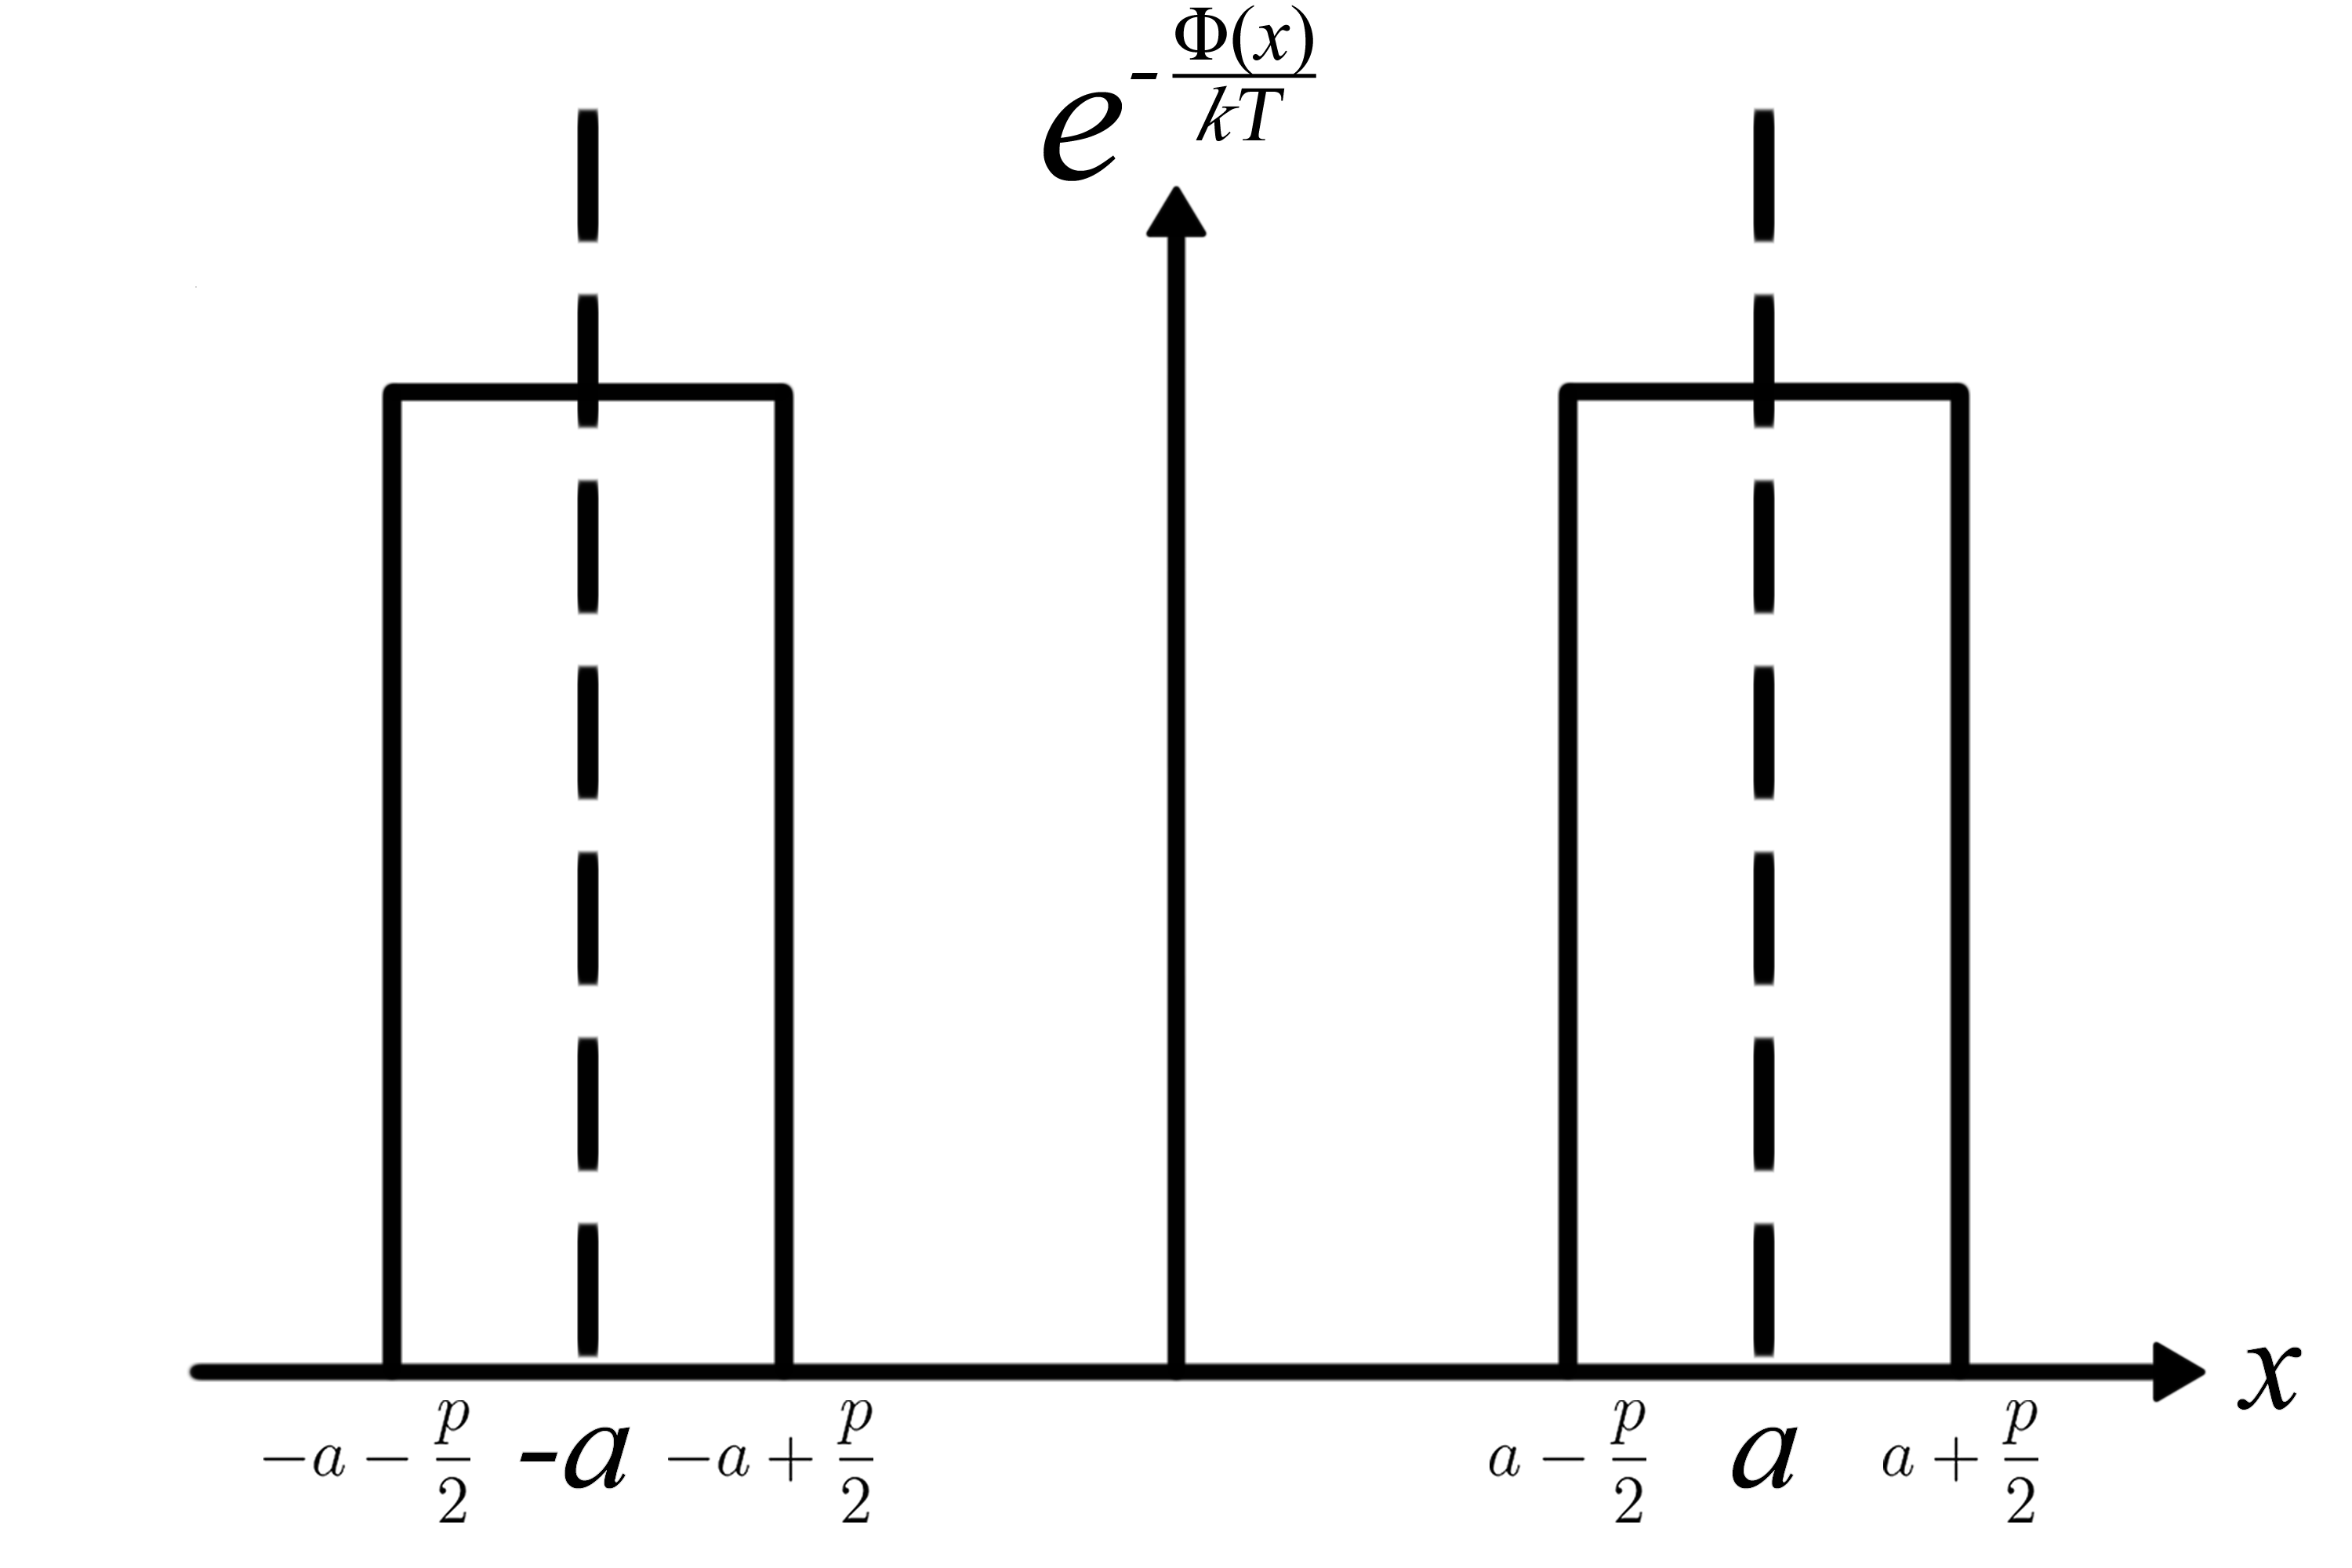
\includegraphics[scale=0.6]{Graphics/DoubleTopHatFunction.png} 
\caption{A plot showing a pair of top-hat functions as the weighting function with
a finite thickness $p$ and finite height. The top-hats are centred about $a$ and $-a$.}
\label{fig:DoubleTophatPotential} 
\end{figure}

\subsection{Extendable Freely Jointed Chain}

Working from \eqref{FourierTransformPartitionFunction} taking our one dimensional model along the $x$-axis in a Cartesian co-ordinate system we have,
%
\begin{equation}
Z_{q}\left(R\right)=\frac{1}{2\pi}\int_{-\infty}^{\infty}d\omega\, e^{-i\omega R}\left[\int_{-\infty}^{\infty}d\Delta x\, e^{-\frac{\Phi\left(\Delta x\right)}{kT}}\, e^{i\omega\Delta x}\right]^{N}\label{FourierTransFormPartitionFunction1D}
\end{equation}
%
We have already obtained the partition function for the FJC by replacing the weighting factor in the integrand with a sum of two delta functions. For a EFJC we will now use two top-hat functions as the weighting factor for the potential, the Fourier transform weighted potential, $G\left(\omega\right)$, is then written as two integrals over finite limits. The Fourier transform of the weighting factor for the EFJC becomes,
%
\begin{align}
G\left(\omega\right) & =\int_{-\infty}^{\infty}\, e^{-\frac{\Phi\left(\Delta x\right)}{kT}}\, e^{i\omega\Delta x}d\Delta x\label{FTWP}\\
 & =\frac{A}{2p}\int_{-a-\frac{p}{2}}^{-a+\frac{p}{2}}e^{i\omega\Delta x}\, d\Delta x+\frac{A}{2p}\int_{a-\frac{p}{2}}^{a+\frac{p}{2}}e^{i\omega\Delta x}\, d\Delta x\\
 & =\left(\frac{2A}{\omega p}\right)\cos\omega a \, \sin \frac{\omega p}{2} \label{FourierTransformWeightedPotential1D}
\end{align}
%
Combining \eqref{FourierTransFormPartitionFunction1D} and \eqref{FourierTransformWeightedPotential1D} gives a simpler expression for the partition function,
%
\begin{equation}
Z_{q}\left(R\right)=\frac{1}{2\pi}\int_{-\infty}^{\infty}d\omega\, e^{-i\omega R}\left[\left(\frac{2A}{\omega p}\right)\cos\omega a\,\sin\frac{\omega p}{2}\right]^{N}\label{PartitionFunctionUnsolved1D}
\end{equation}
%
At this point we can begin to consider how $p$ affects the solution and enquire whether an approximation of small $p$ helps to simplify \eqref{PartitionFunctionUnsolved1D} to produce a neat solution. It is perfectly acceptable to take the small approximation of $p$ since we have stated that the width of the top-hat weighted potential is small and finite. For the EFJC different methods can be used to impose the limit where $p$ becomes finite producing the desired result for $Z_{q}\left(R\right)$. Each method starts from \eqref{PartitionFunctionUnsolved1D}.

\subsection{Imposing the limit of $p$ by the small approximation of $\boldsymbol{\sin\left(\frac{\omega p}{2}\right)}$}

Applying the small approximation of $p$ we linearise the trigonometric function such that $\sin\left(\frac{\omega p}{2}\right)\simeq\frac{\omega p}{2}$ before the integral is evaluated. \eqref{PartitionFunctionUnsolved1D}
becomes,
%
\begin{equation}
Z_{q}\left(R\right)=\frac{A^{N}}{2\pi}\int_{-\infty}^{\infty}e^{-i\omega R}\cos^{N}\omega a\, d\omega\label{pfSmallLimitP}
\end{equation}
%
Then using \eqref{Cos_Series} and the integral representation of the Dirac delta function we recover the partition function for the FJC,
%
\begin{equation}
Z_{q}\left(R\right)=\frac{A^{N}}{2^{N+1}\pi}\sum_{k=0}^{N}\binom{N}{k}\delta\left(R+2k-N\right)
\end{equation}
%
With the small approximation of $p$, we have effectively approximated $G\left(\omega\right)$ to first order which gives the model for a FJC. Next we will include the higher order terms in the expansion
of $\sin\left(\frac{\omega p}{2}\right)$.

\subsection{Using the Taylor expansion of $\sin \frac{\omega p}{2}$ to include higher order terms}

By employing the expansion of $\sin(\frac{\omega p}{2})$ we are including higher order terms in the calculation of $Z_{q}$ before imposing the limit of $p\rightarrow0$. Working from \eqref{PartitionFunctionUnsolved1D} we can write $\cos^{N} \omega a$ as a series of exponentials using \eqref{Cos_Series}. The Taylor expansion of the sine term can be written as
%
\begin{equation}\label{sin_taylor}
\frac{ \sin^{N} \left(\frac{\omega p}{2}\right)}{\left(\frac{\omega p}{2}\right)^{N}} =  \sum_{m=0}^{\infty}A_{m}\left(\omega p \right)^{m}
\end{equation}
%
The partition function for an EFJC then becomes
%
\begin{equation}
Z_{q}\left(R\right)=\frac{A^{N}}{2^{N+1}\pi}\sum_{k=0}^{N}\binom{N}{k}\int_{-\infty}^{\infty}e^{-i\omega\left(R+2k-N\right)}\sum_{m=0}^{\infty}A_{m}\left(\omega p\right)^{m}\, d\omega
\end{equation}
%
The complex integral maybe be written \cite{Bronshtein2007}
%
\begin{equation}
\int_{-\infty}^{\infty}\omega^{b}e^{-i\alpha\omega}\, d\omega=2\pi i^{b}\delta^{(b)}(\alpha)
\end{equation}
%
where $\delta^{(b)}(\alpha)$ is the $b^{th}$ derivative of the delta function. So inserting this solution into the power series we get
%
\begin{equation}
Z_{q}\left(R\right)=\frac{A^{N}}{2^{N+1}\pi}\sum_{k=0}^{N}\binom{N}{k} \sum^{\infty}_{m=0}A_{m}2\pi (ip)^{m}\delta^{m}\left(\alpha\right)
\end{equation}
%
where $\alpha=R+2k-N$. We can then express the differential of the delta functions as,
$\delta^{n}\left(\gamma\right)=\left(-1\right)^{n}n!\delta\left(\gamma\right)/\gamma^{n}$, so
%
\begin{equation}
Z_{q}\left(R\right)=\frac{A^{N}}{2^{N+1}\pi}\sum_{k=0}^{N}\binom{N}{k} \sum^{\infty}_{m=0}G_{m}p^{m}\delta\left(\alpha\right)
\end{equation}
%
where $G_{m} = A_{m}2\pi \left(-i\right)^{m} m!$. Having the Dirac delta function in the result for $Z_{q}$ is important because it shows that only when $\alpha=0$ do we have a non-zero result for the partition function. At this stage we can take the limit of $p\rightarrow0$,
%
\begin{equation}
Z_{q}\left(R\right)=\frac{A^{N}}{2^{N+1}\pi}\sum_{k=0}^{N}\binom{N}{k}\left(G_{0}\delta\left(\alpha\right) + \lim_{p \to 0}\sum^{\infty}_{m=1}G_{m}p^{m}\delta\left(\alpha\right) \right)
\end{equation}
%
which becomes,
%
\begin{equation}
Z_{q}\left(R\right)=\frac{A^{N}}{2^{N+1}\pi}\sum_{k=0}^{N}\binom{N}{k}G_{0}\delta\left(\alpha\right)\label{pfSolved1D_2}
\end{equation}
%
as required, as in \eqref{pfSolved1D_1}. 

Both methods described above yield the same result for the small approximation for $p$, with the solution being the same as the FJC. However, the analysis is somewhat misleading since the general partition function appears to be a modified set of delta functions, rather than a continuous function of $R$. This outcome is a consequence of assuming that the series in $p$ produces convergent integrals which is unclear. In order to obtain the correct partition function for the EFJC we will need to  consider the exact solution of \eqref{PartitionFunctionUnsolved1D}.

\subsection{Expanding the Fourier Transform of the Potential as a Series}

With the Fourier transform of the weighted potential raised to the $N^{th}$ power we can express the trigonometric functions as a series of exponentials with sum over $k^{'}$ and $k$ using the binomial theorem. The expression for $\cos^{N}\left(x\right)$ is given by \eqref{Cos_Series} and the term for $\sin^{N}\left(x\right)$ is given by,
%
\begin{equation}
\sin^{N}x=\frac{1}{(2i)^{N}}\sum_{k^{'}=0}^{N}\binom{N}{k^{'}}(-1)^{k^{'}}e^{ix(N-2k^{'})}\label{Sin_Series}
\end{equation}
%
Using \eqref{Cos_Series} and \eqref{Sin_Series} for the trigonometric terms, \eqref{PartitionFunctionUnsolved1D} becomes
%
\begin{equation}
Z_{q}\left(R\right)=\frac{A^{N}}{2^{N+1}\pi i^N p^{N}}\sum_{k^{\,}=0}^{N}\sum_{{k}'=0}^{N}\binom{N}{k}\binom{N}{k'}\left(-1\right)^{k^{'}}\int_{-\infty}^{\infty}\frac{e^{i\omega\left(a\left(N-2k\right)+\frac{p}{2}\left(N-2{k}'\right)-R\right)}}{\omega^{N}}\, d\omega\label{pfExactUnsolved1D}
\end{equation}
%
The complex multipole integral takes the form,
%
\begin{equation}
\int_{-\infty}^{\infty}\frac{e^{i\omega\zeta}}{\omega^{N}}\, d\omega\,=\frac{\pi i^{N}\zeta^{N-1}}{\left(N-1\right)!}\sgn\left(\zeta\right)\label{MultipoleIntegral}
\end{equation}
%
where
%
\begin{equation}
\sgn\left(\zeta\right)=\begin{cases}
-1 & \text{ for }\zeta<0\\
0 & \text{ for }\zeta=0\\
1 & \text{ for }\zeta>0\end{cases}\label{sign}
\end{equation}
%
Using \eqref{MultipoleIntegral} to evaluate the integral, \eqref{pfExactUnsolved1D} becomes
%
\begin{equation}
Z_{q}\left(R\right)=\frac{A^{N}}{2^{N+1} p^{N}}\sum_{k^{\,}=0}^{N}\sum_{{k}'=0}^{N}\binom{N}{k}\binom{N}{k'}\left(-1\right)^{k^{'}}\frac{\eta^{N-1}}{\left(N-1\right)!}\sgn\left(\eta\right)\label{PartitionFunction1DSolved}
\end{equation}
%
where $\eta=a\left(N-2k\right)+\frac{p}{2}\left(N-2{k}'\right)-R$.

Referring to the case where $N=2$, we see in \figref{1DN2Orig} that the partition function given by \eqref{PartitionFunction1DSolved} is twice as large at $R=0$ than at $R=2$. This is what we expect to find for the FJC chain in 1D. For the case when $N=1$ only one link exists in the FJC which means that the end point can only lie at one of the two positions denoted by $R=1,-1$. A plot of $Z_{q}\left(R\right)$ where $N=1$ and $p=0.1a$ is shown in \figref{1DN1Orig}. For the cases where $N$ is an odd number the partition function at an even position, $k=0,2,4,6,8,..$, will always be zero since the end of the EFJC will never reach those positions unless $p$ is larger.

As the number of links increases in the EFJC we see from \figref{1DN8Orig} and \figref{1DN10Orig} that \eqref{PartitionFunction1DSolved} begins to break down giving irregular results. The nature of this problem is due to the fact that as $N$ gets larger the cancellations due to $\sgn(\eta)$ in the polynomials become extremely delicate. The sums in $Z_{q}\left(R\right)$ for low $N$ involves relevant cancellations to give the required result, as shown in Table. \ref{table:kernal}.

To overcome this problem we can impose constraints from the analysis of \eqref{PartitionFunction1DSolved} to assist with the cancellations that take place. In the polynomial $\eta^{N-1}\sgn\left(\eta\right)$ we will rewrite $\eta$ such that,
%
\begin{equation}\label{eta1}
\eta=F(k,k')-R\end{equation}
%
Where
%
\begin{equation}
F(k,k')=a(N-2k)+\frac{p}{2}(N-2k')\label{Adjustment1}
\end{equation}
%
To impose the correct constraints let us examine in detail the nature of \eqref{PartitionFunction1DSolved}. The partition function is a sum of terms labelled by $k$ and $k'$. We shall refer to $k$ as an index denoting the coarse scale structure of $Z_{q}(R)$ and $k'$ as a label of the fine scale structure for reasons that will become clear later. For a given value of $k$, the core of the expression is
%
\begin{equation}\label{eta2}
\sum_{k'=0}^{N}\left(-1\right)^{k'}\eta^{N-1}\sgn (\eta)
\end{equation}
%
From \eqref{eta1} and \eqref{eta2} we can deduce that for $R < \min_{k'}(F(k,k')) = F(k,N) = a(N-2k)-\frac{Np}{2}$, $\eta > 0$ for all $k'$. Therefore $\sgn\left(\eta\right) = 1$. Hence for $R$ below such a threshold, the core expression reduces to
%
\begin{equation}\label{eta3}
\sum_{k'=0}^{N}\left(-1\right)^{k'}\eta^{N-1}
\end{equation}
%
By writing $\eta$ as $A+Bk'$, the evaluation of \eqref{eta3} requires us to consider
%
\begin{equation}
\sum^{N}_{k'=0}\binom{N}{k'}\left(-1\right)^{k'}k'^{m} 
\end{equation} 
%
with $m$ taking integer values between zero and $N-1$. However, it may be shown that all such summations are zero, for $m < N$. Similarly, for $R> \max_{k'}(F(k,k'))=F(k,0)=a(N-2k)+\frac{Np}{2}$ we find that $\eta<0$ and $\sgn(\eta)=-1$ for all $k'$. Once again the core expression reduces to
%
\begin{equation}
\sum^{N}_{k'=0}\binom{N}{k'}\left(-1\right)^{k'}\eta^{N-1}
\end{equation}
%
and by similar reasoning, this vanishes.

We find, therefore, that contributions to $Z_{q}\left(R\right)$ for a given $k$ in \eqref{PartitionFunction1DSolved} only arise for the region $a(N-2k)-\frac{Np}{2}\leq R \leq a(N-2k)+\frac{Np}{2}$. This corresponds to a region of width $Np$ about a central position $a(N-2k)$. Within this range, a non-zero contribution to $Z_{q}\left(R\right)$ is made from the sum over $k'$, with modulation due to the change in sign of $\eta$ at some point in the sum over $k'$.

Thus each value of $k$ in the expression for $Z_{q}\left(R\right)$ defines a coarse region of $R$ within which non-zero contributions are made due to the summation over $k'$. For this reason we characterise $k$ as the coarse structure label and $k'$ as a fine structure label.

Returning to \eqref{eta2}, we see that it is a sum of polynomials in $R$, of order $N-1$, each with a different zero corresponding to $R=F(k,k')$. For values of $R$  further and further away from each zero, the polynomial $(F(k,k')-R)^{N-1}$ increases rapidly, especially for large $N$ and yet the sum of all the terms vanishes. This is due to a very delicate cancellations of terms. In numerical implementations, such a cancellation will fail in detail, as is shown by the breakdown in the calculation of $Z_{q}\left(R\right)$ for larger $N$ in \figref{1DN8Orig} and \figref{1DN10Orig}. This difficulty, however, may be removed if we help the core expression to vanish for $R$ outside the coarse scale range of values. We multiply it by a top hat function which is zero outside the range $a(N-2k) -\frac{Np}{2} < R < a(N-2k)+\frac{Np}{2}$ and unity within. This function is 
%
\begin{equation}
\Theta(R,k)=H(R-F(k,N))H(F(k,0)-R)\label{AdjustmentTopHat}
\end{equation}
%
and hence the expression for $Z_{q}(R)$ may be revised to,
%
\begin{equation}
Z_{q}\left(R\right)=\frac{A^{N}}{2^{N+1} p^{N}}\sum_{k^{\,}=0}^{N}\sum_{{k}'=0}^{N}\binom{N}{k}\binom{N}{k'}\left(-1\right)^{k^{'}}\frac{\eta^{N-1}}{\left(N-1\right)!}\sgn\left(\eta\right)\Theta(R,k)\label{NewPartitionFunction1DSolved}
\end{equation}
%
A plot of the partition function using \eqref{NewPartitionFunction1DSolved} can be seen in \figref{Z1D}. For the specific cases where $N=8$ and $N=10$ we can see that \figref{1DN8} and \figref{1DN10} show stable results. A detailed breakdown of the modified partition function for $N=2$ is shown in Table. \ref{table:mod_kernal}.

\renewcommand{\arraystretch}{1.5}
\begin{table}[h]
\centering
    \begin{tabular}{ c c c } \hline
    $R$ & $\binom{N}{k}\binom{N}{k'}\left(-1\right)^{k^{'}}\frac{\eta^{N-1}}{\left(N-1\right)!}\sgn\left(\eta\right)$ & $\sum_{k,k'}^{N}\binom{N}{k}\binom{N}{k'}\left(-1\right)^{k^{'}}\frac{\eta^{N-1}}{\left(N-1\right)!}\sgn\left(\eta\right)$ \\ [1ex] \hline\hline 
    -2  & \{4.2,\,-8,\,3.8,\,4.4,\,-8,\,3.6\},\,0.2,\,0,\,0.2  & 0.4 \\ 
    -1  & \{3.2,\,-6,\,2.8,\,2.4,\,-4,\,1.6,\,0.8,\,-2,\,1.2\} & 0   \\ 
    0   & \{2.2,\,-4,\,1.8\},\,0.4,\,0,\,0.4,\,\{1.8,\,-4,\,2.2\}  & 0.8 \\ 
    1   & \{1.2,\,-2,\,0.8,\,1.6,\,-4,\,2.4,\,2.8,\,-6,\,3.2\} & 0   \\ 
    2   & 0.2,\,0,\,0.2,\,\{3.6,\,-8,\,4.4,\,3.8,\,-8,\,4.2\}  & 0.4 \\ [1ex] \hline
    \end{tabular}
\caption{A breakdown of the partition function \eqref{PartitionFunction1DSolved} for N=2. The relevant summations in the curly brackets are the cancellations that occur in the partition to give a desired result. For small $N$ these cancellations are simple which become more difficult for larger $N$. This is seen in \figref{1DN10Orig}.}
\label{table:kernal}
\end{table}

\begin{table}[h]
\centering
    \begin{tabular}{ c c c } \hline
    $R$ & $\binom{N}{k}\binom{N}{k'}\left(-1\right)^{k^{'}}\frac{\eta^{N-1}}{\left(N-1\right)!}\sgn\left(\eta\right)\Theta(R,k)$ & $\sum_{k,k'}^{N}\binom{N}{k}\binom{N}{k'}\left(-1\right)^{k^{'}}\frac{\eta^{N-1}}{\left(N-1\right)!}\sgn\left(\eta\right)\Theta(R,k)$ \\ [1ex] \hline\hline 
    -2  & \{0,\,0,\,0,\,0,\,0,\,0\},\,0.2,\,0,\,0.2  & 0.4 \\ 
    -1  & \{0,\,0,\,0,\,0,\,0,\,0,\,0,\,0,\,0\} & 0   \\ 
    0   & \{0,\,0,\,0\},\,0.4,\,0,\,0.4,\,\{0,\,0,\,0\}  & 0.8 \\ 
    1   & \{0,\,0,\,0,\,0,\,0,\,0,\,0,\,0,\,0\} & 0   \\ 
    2   & 0.2,\,0,\,0.2,\,\{0,\,0,\,0,\,0,\,0,\,0\}  & 0.4 \\ [1ex] \hline
    \end{tabular}
\caption{A breakdown of the modified partition function \eqref{NewPartitionFunction1DSolved} for N=2. The values that contributed to the cancellations in the partition function \eqref{PartitionFunction1DSolved} have been set to zero by the function $\Theta$. Only values that contribute to the overall partition function are included in the summations. This works for all N.}
\label{table:mod_kernal}
\end{table}


\begin{figure}[htp]
\centering
\begin{tabular}{cc}
\subfloat[N=1]{\label{fig:1DN1Orig}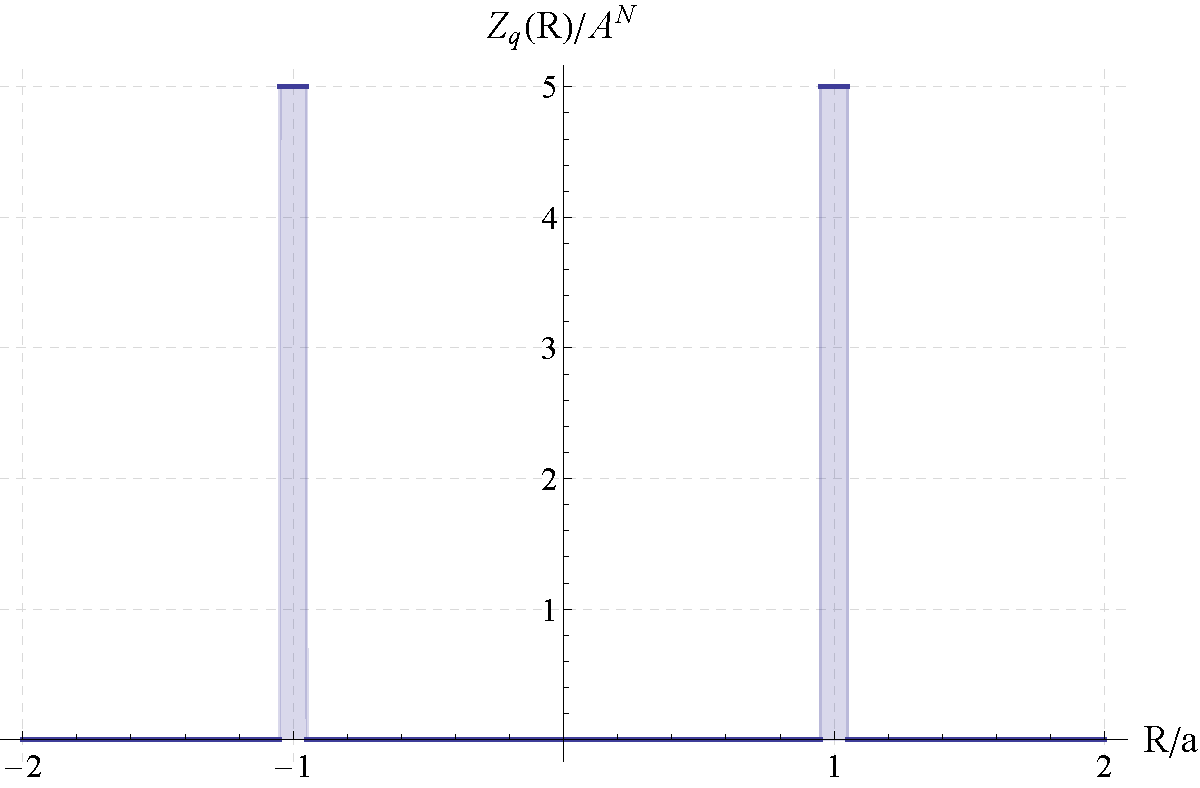
\includegraphics[scale=0.35]{Graphics/1D/Original/1D_N1_Orig.pdf}} &
\subfloat[N=2]{\label{fig:1DN2Orig}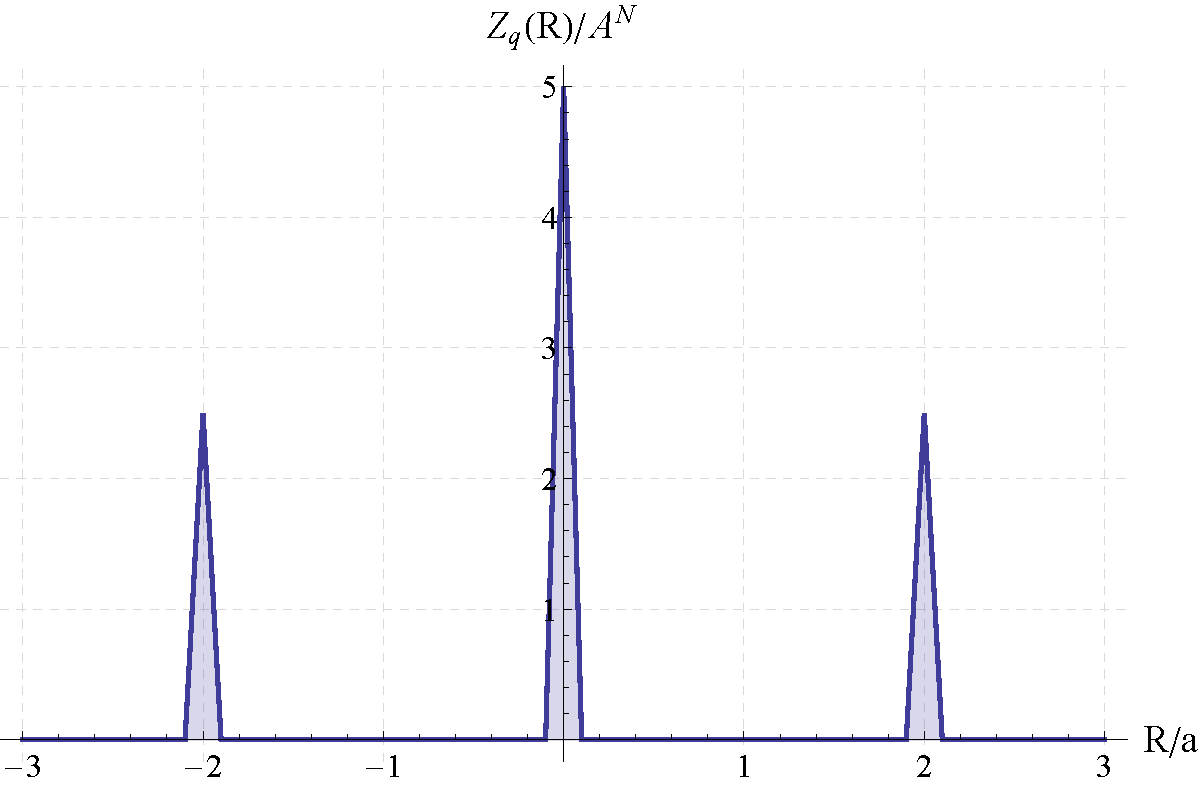
\includegraphics[scale=0.35]{Graphics/1D/Original/1D_N2_Orig.pdf}} \\
\subfloat[N=4]{\label{fig:1DN4Orig}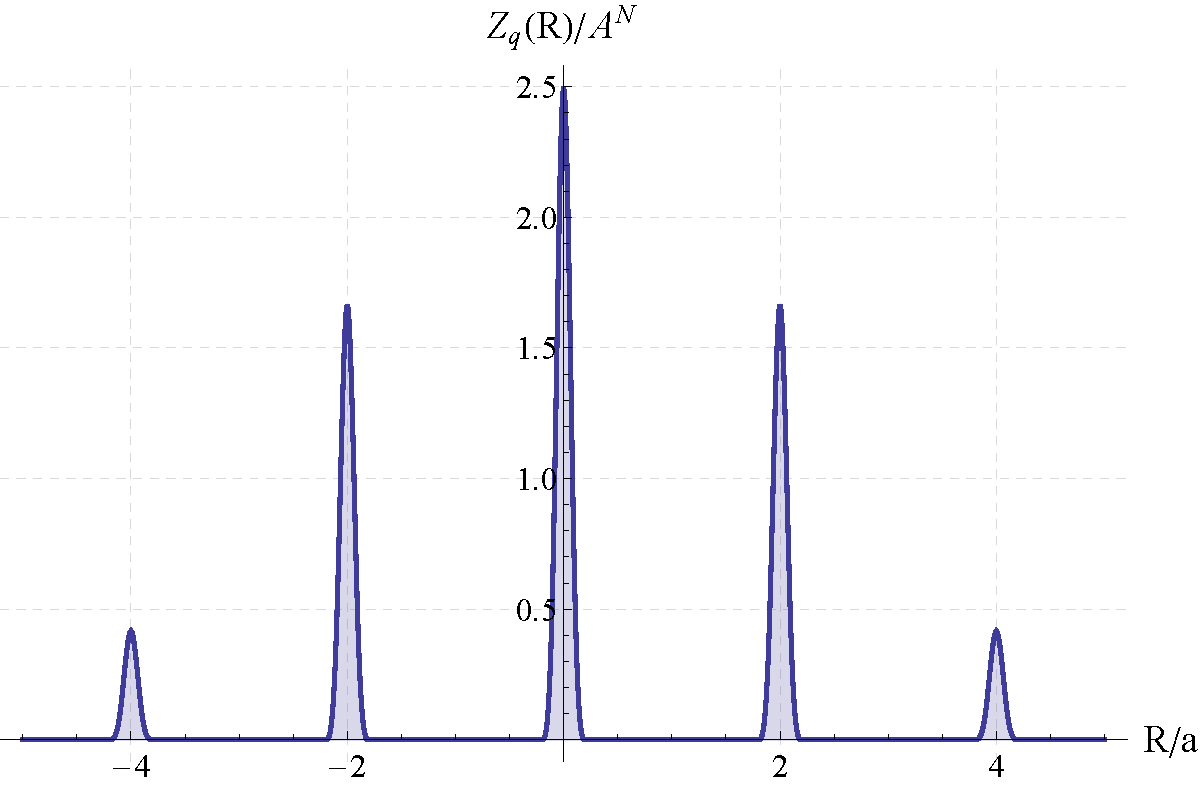
\includegraphics[scale=0.35]{Graphics/1D/Original/1D_N4_Orig.pdf}} &
\subfloat[N=6]{\label{fig:1DN6Orig}\includegraphics[scale=0.35]{Graphics/1D/Original/1D_N6_Orig.pdf}} \\
\subfloat[N=8]{\label{fig:1DN8Orig}\includegraphics[scale=0.35]{Graphics/1D/Original/1D_N8_Orig.pdf}} &
\subfloat[N=10]{\label{fig:1DN10Orig}\includegraphics[scale=0.35]{Graphics/1D/Original/1D_N10_Orig.pdf}}
\end{tabular} 
\caption{Plots showing the partition function for an extendable FJC with $p=0.1a$. The original partition function used to plot these graphs \eqref{PartitionFunction1DSolved}. Notice the breakdown in the calculations for $N=10$.}
\label{fig:Z1DOrig} 
\end{figure}

\begin{figure}[htp]
\centering
\begin{tabular}{cc}
\subfloat[N=1]{\label{fig:1D_N1}\includegraphics[scale=0.35]{Graphics/1D/1D_N1.pdf}} &
\subfloat[N=2]{\label{fig:1DN2}\includegraphics[scale=0.35]{Graphics/1D/1D_N2.pdf}} \\
\subfloat[N=4]{\label{fig:1DN4}\includegraphics[scale=0.35]{Graphics/1D/1D_N4.pdf}} &
\subfloat[N=6]{\label{fig:1DN6}\includegraphics[scale=0.35]{Graphics/1D/1D_N6.pdf}} \\
\subfloat[N=8]{\label{fig:1DN8}\includegraphics[scale=0.35]{Graphics/1D/1D_N8.pdf}} &
\subfloat[N=10]{\label{fig:1DN10}\includegraphics[scale=0.35]{Graphics/1D/1D_N10.pdf}}
\end{tabular} 
\caption{Plots showing the partition function for an extendable FJC with $p=0.1a$. The partition
function used to plot these graphs has been modified with the insertion of the top-hat function $\Theta(R,k)$. Notice that the failure to cancel terms in the expression has been avoided and the calculation for N=10 converges.}
\label{fig:Z1D} 
\end{figure}

\newpage
\section{Extendable Freely Jointed Chain in Three Dimensions}

Evaluating the partition function for a one dimensional EFJC gave an expression for $Z_{q}(R)$ which with slight adjustment worked well to give a probability density distribution for the end-to-end separation of the EFJC. In the small approximation of $p$, we saw that the behaviour of $Z_{q}$ tended towards that of a non-extendable FJC, consistent with the treatment of the FJC as a one dimensional random walk. Modelling the FJC as a stochastic process we were able to determine an expectation of $R$. The results were consistent with each other. The next stage is to take a 3-D realisation of the EFJC model, allowing each link to move independently in three spatial dimensions, employing a finite potential to characterise the links.

\subsection{Construction of the Partition Function}

In three dimensional space the current partition function integral is inadequate as it has been constructed in the Cartesian co-ordinate system. A better method would be to employ spherical co-ordinates where one end of the EFJC is fixed at the origin. We have
%
\begin{equation}
Z_{q}=\int \prod_{i=1}^{N}d^{3}\boldsymbol{r}_{i} \exp\left(-\frac{\Phi\left(\{\boldsymbol{r}_{i}\}\right)}{kT}\right)
\end{equation}
%
Each link in the 3D EFJC will be characterised by a potential which is function of $\boldsymbol{r}_{i,i-1}=\boldsymbol{r}_{i}-\boldsymbol{r}_{i-1}$, with $\boldsymbol{r}_{0}=0$, which allows it to extend or contract by a finite length $\frac{p}{2}$. This allows the potential, $\Phi$, to separate such that
%
\begin{equation}
\Phi\left(\{\boldsymbol{r}_{i}\}\right) = \sum_{i=1}^{N}\phi\left(\boldsymbol{r}_{i,i-1}\right)
\end{equation}
%
Inserting the constraint $\boldsymbol{r}'=\sum_{i=1}^{N}\boldsymbol{r}_{i,i-1}$ through a delta function, we fix the total vector sum of all the particle separations. We then define
%
\begin{equation}
Z_{q}\left(\boldsymbol{r}'\right)=\int\prod_{i=1}^{N}d^{3}\boldsymbol{r}_{i,i-1}\,\delta^{3}\left(\boldsymbol{r'}-\sum_{i=1}^{N}\boldsymbol{r}_{i,i-1}\right)\prod_{i=1}^{N} \exp\left(-\frac{\phi\left(\boldsymbol{r}_{i,i-1}\right)}{kT}\right)\label{pf3d1}
\end{equation}
%
such that $Z_{q}=\int Z_{q}\left(\boldsymbol{r}'\right)d^{3}\boldsymbol{r}'$.

Intuitively, we expect $Z_{q}\left(\boldsymbol{r}'\right)$ to depend on $R=|\boldsymbol{r}'|$ only. It counts the (weighted) numbers of configurations with polymer vector length $\boldsymbol{r}'$, and the orientation of $\boldsymbol{r}'$ does not alter this count. The probability distribution of the length $R$ is actually
%
\begin{equation}
P_{N}\left(R\right)= \frac{R^{2}Z_{q}\left(R\right)}{\int R^{2}Z_{q}\left(R\right)dR}
\end{equation}
%
which is correctly normalised such that $\int^{\infty}_{0} P_{N}\left(R\right)dR=1$. Using the integral representation of the delta function constraint as
%
\begin{equation}\label{pf3d_delta}
\delta\left(\boldsymbol{r}'-\sum_{i=1}^{N}\boldsymbol{r}_{i,i-1}\right)=\frac{1}{\left(2\pi\right)^{3}}\int d^{3}\boldsymbol{k}\, \exp\left(-i\boldsymbol{k}.\left(\boldsymbol{r}'-\sum_{i=1}^{N}\boldsymbol{r}_{i,i-1}\right)\right)
\end{equation}
%
and inserting it into \eqref{pf3d1} we obtain
%
\begin{equation}\label{pf3draw}
Z_{q}\left(\boldsymbol{r}'\right) = \frac{1}{\left(2\pi\right)^{3}}\int d^{3}\boldsymbol{k}\, \exp\left(-i\boldsymbol{k}.\boldsymbol{r}'\right)\left(\int_{-\infty}^{\infty}d^{3}\boldsymbol{r}_{i,i-1}\, \exp\left(-\frac{\phi\left(\boldsymbol{r}_{i,i-1}\right)}{kT}\right)\exp\left(i\boldsymbol{k}.\boldsymbol{r}_{i,i-1}\right) \right)^{N}
\end{equation}
%
Representing the Fourier transform of the weighting function as $F\left(\boldsymbol{k}\right)$, we can simplify \eqref{pf3draw} so that it becomes a function of $R$,
%
\begin{align}
Z_{q}\left(R\right) &= \frac{1}{\left(2\pi\right)^{3}}\int_{0}^{\infty}k^{2}\left(2\pi\int_{-1}^{1} e^{-ikR\cos \theta} d\left(\cos \theta \right)\right)dk\, F^{N}\left(\boldsymbol{k}\right) \\
&= \frac{1}{\left(2\pi\right)^{2}}\int_{0}^{\infty}dk\frac{k}{R}\sin kR\, F^{N}\left(\boldsymbol{k}\right)\label{PartitionFunctionUnsolved3D} 
\end{align}
%
where the Fourier transform integral $F\left(\boldsymbol{k}\right)$ is
%
\begin{equation}
F\left(\boldsymbol{k}\right)=\int_{-\infty}^{\infty}d^{3}\boldsymbol{r}_{i,i-1}\, \exp\left(-\frac{\phi\left(\boldsymbol{r}_{i,i-1}\right)}{kT}\right)\exp\left(i\boldsymbol{k}.\boldsymbol{r}_{i,i-1}\right)\label{FTPI_3D}
\end{equation}
%
Using this general expression for $Z_{q}\left(R\right)$ any potential may be studied.  

\subsection{Evaluating $\boldsymbol{Z_{q}}$ for the non-extendable Freely Jointed Chain}

We previously calculated the partition function for a FJC in one dimension using two delta functions as the weighting factor. Performing the calculation in three dimensions
the analogous potential as a function of $r = |\boldsymbol{r}_{i,i-1}|$ is
%
\begin{equation}
\phi\left(\boldsymbol{r}_{i,i-1}\right)=-kT\ln\left(D\delta\left(r-a\right)\right)\label{FJC3D}
\end{equation}
%
Where $D$ is a constant with dimensions of length. Inserting \eqref{FJC3D} into \eqref{FTPI_3D} we get
%
\begin{align}
F\left(\boldsymbol{k}\right) & =\int_{-\infty}^{\infty}\int_{-\infty}^{\infty}\int_{-\infty}^{\infty}\, d^{3}\boldsymbol{r}\,D\delta\left(r-a\right)\exp\left(-i\boldsymbol{k.r}\right)\nonumber\\
 & =D\int_{-1}^{1}2\pi d\left(\cos\theta\right)\int_{0}^{\infty}\delta\left(r-a\right)r^{2}\exp\left(-ikr\cos\theta\right)dr\nonumber\\
 & =D\int_{0}^{\infty}\delta\left(r-a\right)\frac{4\pi r}{k}\sin kr\,dr\label{FJC_FTP_Unsolved}
\end{align}
%
Such that the Fourier transform of the exponentiated potential for a FJC becomes
%
\begin{equation}
F\left(k\right)=\left(\frac{4\pi a D}{k}\right)\sin ka\label{FourierTransformPotentialWeighted}
\end{equation}
%
Inserting \eqref{FourierTransformPotentialWeighted} into \eqref{PartitionFunctionUnsolved3D}
the partition function integral becomes
%
\begin{equation}
Z_{q}\left(R\right) = \frac{\left(4 \pi a D\right)^{N}}{4\pi^{2}R} \int_{0}^{\infty}\frac{\sin kR \sin^{N}ka}{k^{N-1}}\,dk
\end{equation}
%
and using \eqref{Sin_Series} to express $\sin^{N}ka$ as a sum of exponentials and $\sin kR$ as the real part of $ie^{-ikR}$ the partition function becomes
%
\begin{equation}
Z_{q}\left(R\right) = \frac{\left(4 \pi a D\right)^{N}i}{4\pi^{2}R \left(2i\right)^{N}}\sum^{N}_{l=0}\binom{N}{l}\left(-1\right)^{l}\int^{\infty}_{0}\frac{e^{ik\left(a\left(N-2l\right)-R\right)}}{k^{N-1}}\,dk
\end{equation}
%
Since the integral has already been calculated in \eqref{MultipoleIntegral}, the solution for a FJC in 3-D becomes
%
\begin{equation}
Z_{q}\left(R\right)=\frac{\left(2\pi a D\right)^{N}}{4\pi R\left(N-2\right)!}\sum_{l=0}^{N}\binom{N}{l}\left(-1\right)^{l}\left[a\left(N-2l\right)-R\right]^{N-2}\sgn\left(a\left(N-2l\right)-R\right)\label{PartitionFunction3DFJC}
\end{equation}

\subsection{The Shell Potential and its Fourier Transform}

In the 1-D model we saw that a double top-hat weighting function was able to generate the partition function for an EFJC. In three dimensions, due to the rotational symmetry the potential is only dependent on the $r$ co-ordinate. A potential that is non-zero only within the range of $r$ at $a-\frac{p}{2}\leq r\leq a+\frac{p}{2}$ gives a weighting function that can be viewed as a shell with a thickness of length $p$.

Working with the partition function, let us insert $\exp\left(-\phi\left(r\right)/kT\right)=C$ for $a-\frac{p}{2}\leq r\leq a+\frac{p}{2}$, and zero elsewhere, $\exp\left(-\phi\left(r\right)/kT\right)=0$, where $C$ is a dimensionless constant. Contributions to the partition function arise only where the potential is finite so the exponentiated potential Fourier transform integral simplifies to
%
\begin{equation}
F\left(k\right)=C\int_{\cos\theta=-1}^{1}2\pi d\left(\cos\theta\right)\int_{a-\frac{p}{2}}^{a+\frac{p}{2}}r^{2}dr\, e^{ikr\cos\theta}
\end{equation}
%
This result was obtained by using $d^{3}\boldsymbol{r}=d\phi\sin\theta d\theta r^{2}dr$ and rewriting $\sin\theta d\theta$ as $-d\left(\cos\theta\right)$. Performing the integral with respect to $r$ in the potential range
we have the final result
%
\begin{equation}
F\left(k\right)=\frac{4\pi C}{k^{2}}\left(\frac{2\cos ka\sin\frac{kp}{2}}{k}+2a\sin ka\sin\frac{kp}{2}-p\cos ka\cos\frac{kp}{2}\right)\label{PotentialTerm3D}
\end{equation}
%
With this expression for $F\left(k\right)$ the final partition function for a EFJC can be analytical evaluated in 3-D.

\subsection{Evaluation of the Partition Function by the small $p$ approximation}

In the small $p$ approximation we once again insert Taylor expansions of all the trigonometric functions in the Fourier transform potential with respect to $p$. For small $p$ in \eqref{PotentialTerm3D} we have a much simpler equation for $F\left(k\right)$
%
\begin{equation}
F\left(k\right)=C\left(\frac{4\pi a p}{k}\right)\sin ka\label{PotentialTerm3DApprox}
\end{equation}
%
Using \eqref{PotentialTerm3DApprox} with \eqref{PartitionFunctionUnsolved3D}
we get
%
\begin{equation}
Z_{q}\left(R\right)=\frac{\left(4\pi a p C\right)^{N}}{2\pi^{2}R}\int_{-\infty}^{\infty}\frac{\sin kR}{k^{N-1}}\sin^{N}ka\, dk
\end{equation}
%
Which evaluates to give
%
\begin{equation}
Z_{q}\left(R\right)=\frac{\left(2\pi a p C\right)^{N}}{2\pi R\left(N-2\right)!}\sum_{l=0}^{N}\binom{N}{l}\left(-1\right)^{l}\left[a\left(N-2l\right)-R\right]^{N-2}\sgn\left(a\left(N-2l\right)-R\right)\label{PartitionFunction3DSmallp}
\end{equation}
%
From the plot in \figref{PF3D} we see that in the large $N$ limit the partition function with constrained end-to-end separation $R$ gives a distribution that peaks about the origin. This is expected for the behaviour of
a FJC. \figref{PF3Dn} shows the probability density function of the end-to-end separation. 
%
\begin{figure}[htp]
 \centering \includegraphics[scale=0.6]{Graphics/PartitionFunction3D.pdf} 
\caption{A plot of \eqref{PartitionFunction3DFJC} for $N=6,10$.}
\label{fig:PF3D} 
\end{figure}

\begin{figure}[htp]
\centering \includegraphics[scale=0.6]{Graphics/PartitionFunction3Dn.pdf} 
\caption{A plot of \eqref{PartitionFunction3DFJC} multiplied by $4\pi R^{2}$
for $N=4,6,8,10$.}
\label{fig:PF3Dn} 
\end{figure}

\subsection{Evaluating the Partition Function for arbitrary $p$}

In the previous section we saw that when the small $p$ approximation was applied to the EFJC in one dimension the resulting partition function became a description of the FJC, a similar case was seen when the small approximation was made in three dimensions. Let us now evaluate the partition function for the EFJC without approximation. We have the Fourier transform as an exact expression, and to combine the various terms into a single complex integral we can first use the binomial theorem to collect the terms which have different factors of $\frac{1}{k}$
%
\begin{equation}
F^{N}(k)=\left(2\pi C\right)^{N}\sum_{\alpha=0}^{N}\binom{N}{\alpha}\frac{1}{i^{\alpha}}\frac{1}{k^{2N+\alpha}}X^{\alpha}Y^{N-\alpha}
\end{equation}
%
where
%
\begin{equation}
X=e^{ik\left(a+\frac{p}{2}\right)}-e^{ik\left(a-\frac{p}{2}\right)}+e^{ik\left(-a+\frac{p}{2}\right)}-e^{ik\left(-a-\frac{p}{2}\right)}
\end{equation}
%
and
%
\begin{equation}
Y=\left(-a-\frac{p}{2}\right)e^{ik\left(a+\frac{p}{2}\right)}-\left(-a+\frac{p}{2}\right)e^{ik\left(a-\frac{p}{2}\right)}+\left(a-\frac{p}{2}\right)e^{ik\left(-a+\frac{p}{2}\right)}-\left(a+\frac{p}{2}\right)e^{ik\left(-a-\frac{p}{2}\right)}
\end{equation}
%
The multinomial theorem is then used for the $X^{\alpha}$ and $Y^{N-\alpha}$ terms. This approach reduces the terms to a single exponent as a function of $k$ such that the integral over $dk$ is simplified. Combining this result with \eqref{PartitionFunctionUnsolved3D} we get a final expression for $Z_{q}$ as
%
\begin{equation}
Z_{q}(R)=\frac{\pi \left(-1\right)^{N}\left(2\pi\right)^{N-2}C^{N}}{R}\sum_{\alpha=0}^{N}\binom{N}{\alpha}\frac{1}{\left(2N+\alpha-2\right)!}\sum_{j_{1},j_{2},j_{3},j_{4}}^{\alpha}\sum_{l_{1},l_{2},l_{3},l_{4}}^{N-\alpha}I\left(N,\alpha,a,p,R,\{j\},\{l\}\right)
\label{PartitionFunctionFiniteP}
\end{equation}
%
with
%
\begin{multline}
I\left(N,\alpha,a,p,R,\{j\},\{l\}\right)=\binom{N}{j_{1},j_{2},j_{3},j_{4}}\binom{N-\alpha}{l_{1},l_{2},l_{3},l_{4}}\left(-1\right)^{j_{2}+j_{4}}\left(-a-\frac{p}{2}\right)^{l_{1}+l_{4}} \times \\ \left(a-\frac{p}{2}\right)^{l_{2}+l_{3}}\left(J\left(a,p,\{j\}\right)+L\left(a,p,\{l\}\right)-R\right)^{2N+\alpha-2}\sgn\left(J\left(a,p,\{j\}\right)+L\left(a,p,\{l\}\right)-R\right)
\end{multline}
%
and
%
\begin{eqnarray*}
\binom{N}{j_{1},j_{2},j_{3},j_{4}}&=&\frac{N!}{j_{1}!\,j_{2}!\,j_{3}!\,j_{4}!} \\
\binom{N-\alpha}{l_{1},l_{2},l_{3},l_{4}}&=&\frac{\left(N-\alpha\right)!}{l_{1}!\,l_{2}!\,l_{3}!\,l_{4}!}
\end{eqnarray*}
%
\begin{eqnarray*}
L\left(a,p,\{l\}\right)&=&\left(a+\frac{p}{2}\right)\left(l_{1}-l_{4}\right)+\left(a-\frac{p}{2}\right)\left(l_{2}-l_{3}\right) \\
J\left(a,p,\{j\}\right)&=&\left(a+\frac{p}{2}\right)\left(j_{1}-j_{4}\right)+\left(a-\frac{p}{2}\right)\left(j_{2}-j_{3}\right)
\end{eqnarray*}
%
\begin{eqnarray*}
\sum^{4}_{k=1}j_{k}&=&N \\
\sum_{k=1}^{4}l_{k}&=&N-\alpha
\end{eqnarray*}
%
A plot of \eqref{PartitionFunctionFiniteP} in \figref{Z3DMultigraphNormailsed} shows
the probability distributions for $N=3,4,5,6$. As $N$ increases in \figref{Z3D} we see that the distributions increasingly centre around $r=0$. \figref{3D_N5} show results for large $N$, where we begin to see that the results become unstable just like in \figref{1DN8Orig}.

\begin{figure}[H]
\includegraphics[scale=0.8]{Graphics/3D/MultigraphFinitePSmall.pdf}
\caption{A plot of normalised partition functions for an extendable FJC in three dimensions. The plot shows distributions for $N=3,4,5,6$ with $p=0.1a$.}
\label{fig:Z3DMultigraphNormailsed}
\end{figure}

\begin{figure}[H]
\centering
\begin{tabular}{cc}
\subfloat[N=1]{\label{fig:3D_N1}\includegraphics[scale=0.45]{Graphics/3D/FinitePSmall/1.pdf}} &
\subfloat[N=2]{\label{fig:3D_N2}\includegraphics[scale=0.45]{Graphics/3D/FinitePSmall/2.pdf}} \\
\subfloat[N=3]{\label{fig:3D_N3}\includegraphics[scale=0.45]{Graphics/3D/FinitePSmall/3.pdf}} &
\subfloat[N=4]{\label{fig:3D_N4}\includegraphics[scale=0.45]{Graphics/3D/FinitePSmall/4.pdf}} \\
\subfloat[N=5]{\label{fig:3D_N5}\includegraphics[scale=0.45]{Graphics/3D/FinitePSmall/5.pdf}} &
\subfloat[N=6]{\label{fig:3D_N6}\includegraphics[scale=0.45]{Graphics/3D/FinitePSmall/6.pdf}} 
\end{tabular} 
\caption{Plots showing the partition function for an extendable FJC in three dimensions with $p=0.1a$.}
\label{fig:Z3D}
\end{figure}

\begin{comment}
\begin{figure}[H]
\centering
\begin{tabular}{cc}
\subfloat[N=1]{\label{fig:3D_N1Large}\includegraphics[scale=0.45]{Graphics/3D/FinitePLarge/1.pdf}} &
\subfloat[N=2]{\label{fig:3D_N2Large}\includegraphics[scale=0.45]{Graphics/3D/FinitePLarge/2.pdf}} \\
\subfloat[N=3]{\label{fig:3D_N3Large}\includegraphics[scale=0.45]{Graphics/3D/FinitePLarge/3.pdf}} &
\subfloat[N=4]{\label{fig:3D_N4Large}\includegraphics[scale=0.45]{Graphics/3D/FinitePLarge/4.pdf}} \\
\subfloat[N=5]{\label{fig:3D_N5Large}\includegraphics[scale=0.45]{Graphics/3D/FinitePLarge/5.pdf}} &
\subfloat[N=6]{\label{fig:3D_N6Large}\includegraphics[scale=0.45]{Graphics/3D/FinitePLarge/6.pdf}} 
\end{tabular} 
\caption{Plots showing the partition function for an extendable FJC in three dimensions with $p=0.5a$.}
\label{fig:Z3DLarge}
\end{figure}
\end{comment}

\begin{figure}[H]
\centering
\begin{tabular}{cc}
\subfloat[p=0.1a]{\label{fig:3D_com01}\includegraphics[scale=0.45]{Graphics/3D/Comparison/4_p01.pdf}} &
\subfloat[p=0.2a]{\label{fig:3D_com02}\includegraphics[scale=0.45]{Graphics/3D/Comparison/4_p02.pdf}} \\
\subfloat[p=0.3a]{\label{fig:3D_com03}\includegraphics[scale=0.45]{Graphics/3D/Comparison/4_p03.pdf}} &
\subfloat[p=0.4a]{\label{fig:3D_com04}\includegraphics[scale=0.45]{Graphics/3D/Comparison/4_p04.pdf}} \\
\subfloat[p=0.5a]{\label{fig:3D_com05}\includegraphics[scale=0.45]{Graphics/3D/Comparison/4_p05.pdf}} &
\subfloat[p=0.6a]{\label{fig:3D_com06}\includegraphics[scale=0.45]{Graphics/3D/Comparison/4_p06.pdf}}
\end{tabular} 
\caption{These plots show a comparison of the probability distribution for the FJC \eqref{PartitionFunction3DSmallp} (blue curve) and the EFJC \eqref{PartitionFunctionFiniteP} (red curve) for different values of $p$ with $N=4$.}
\label{fig:Comparison3D}
\end{figure}
\newpage
\begin{comment}
\begin{figure}[H]
\includegraphics[scale=0.8]{Graphics/3D/PN_finitep05_N5.pdf}
\caption{A plot of the probability distribution of a EFJC ending at a position $R/a$ for $N=5$.}
\end{figure}
\end{comment}

\section{Conclusion}

Using the Fourier Transform Integral method we have presented a model which gives a partition function to describe an Extendable Freely Jointed Chain as an improvement to the non-extendable Freely Jointed Chain. The EFJC improves the standard FJC polymer model by allowing each link in the chain to extend and contract independently to emulate the mechanical behaviour of intermolecular bonds within polymers. 

In one dimension, the partition function for EFJC was calculated using two top-hat functions as the weighting function in the Fourier Transform integral. This potential allowed each link to move freely in one dimension that included a weighting function to provide linear extensibility. Taking a small approximation of $p$ in the EFJC model transformed the partition function to that of a FJC which was calculated using delta functions as the weighting functions. 

In \figref{Comparison3D} we see a plot which compares the results of $Z_{q}$ with N=4 for the FJC and the EFJC with different $p$. It is interesting to note that for extensions where the range of $p$ is less than $0.2a$ the results are almost identical. Above this range we see that the partition function distribution becomes larger in the EFJC model. 

With the negligible differences in the partition function distributions for small $p$ we can conclude that results from the EFJC can be well represented by those from the FJC.

%However, the EFJC holds true where the elasticity is linear, so determining the range of $p$ at which the behaviour stays linear would need to be taken into account as results for $p$ larger than $0.2a$ begin to differ significantly. 

%Extending this work further where more complex strutuces of polymers are involved, a more powerful and general method such as the Transfer Integral method will be used to calculate the partition function. The structure we will be focusing on is the collagen polymer which is a triple helix structure with hydrogen bonds between three component strands.
 


\chapter{DNA Model}

The complex structure of DNA allows external forces to be applied in various ways. In cells, DNA is constantly twisted, bent and stretched by numerous proteins for biological processes and therefore to create a mathematical model that encompasses all these actions would be extremely difficult.

Our DNA model focuses on a shearing force applied to DNA. It specifically looks at the behaviour of the hydrogen bonding between the base pairs under strain and evaluates the free energy of different breakage patterns. The statistical model is in the form of a partition function \eqref{partition_function} where the multi-dimensional integral over phase-space is evaluated by the use of the Transfer Matrix Method. We begin by analysing the Hamiltonian for our DNA model.

\section{Construction of the Hamiltonian}

To form a tractable mathematical model using the transfer matrix method we simplify the double helix structure to a one dimensional ladder structure allowing us to introduce a suitable Hamiltonian. This basic structure is similar to the one first used by de Gennes \cite{DeGennes2001}. The ball and stick diagram of the ladder structure consists of two rows of regularly spaced particles connected by elastic springs \figref{dna_model_ladder}. The springs along the two rows which represent the backbone strands in DNA have a spring constant $\kappa$, and the springs perpendicular to the backbones, representing the base pairs, are harmonic for small extensions with a spring constant $\kappa'$. In this model we will neglect the torsional effects in DNA. The load on the ladder structure will be applied by keeping one end of one of the backbones fixed while the other end of the other backbone is extended axially by a distance $u$.

\begin{figure}
\centering \includegraphics[scale=0.3]{Graphics/DNA_Model/dna_model_ladder.pdf}
\caption{Schematic diagram of the two dimensional ladder model for DNA.}
\label{fig:dna_model_ladder}
\end{figure}

Each particle in the ladder structure represents a nucleotide. Each stick connecting the base pairs represents the 2-3 hydrogen bonds, and each stick along the backbone represents a peptide bond connecting the nucleotides. The axial displacements of particles in each backbone are labelled $x_i$ and $y_i$, and the partners forming the $i^{th}$ base pair interact through a potential $V_{i}$ which is dependent on the axial pair separation $(x_{i}-y_{i})$. For a model that has $N$ base pairs we can write the Hamiltonian as
%
\begin{equation}
\label{dna_hamiltonian}
H = H_{x} + H_{y} + H_{bp}
\end{equation}
%
where
%
\begin{align}
\label{dna_hamiltonian_x}
H_{x} &= \sum_{i=1}^{N-1} \frac{1}{2} \kappa \left(x_{i+1}-x_{i} \right)^2 \\
\label{dna_hamiltonian_y}
H_{y} &= \sum_{i=1}^{N-1} \frac{1}{2} \kappa \left(y_{i+1}-y_{i} \right)^2 \\
\label{dna_hamiltonian_bp}
H_{bp} &= \sum_{i=1}^{N}V_{i}\left(x_{i}-y_{i}\right)
\end{align}
%
To eliminate the cross terms in the Hamiltonian we change the co-ordinate system of variables $x_{i}$ and $y_{i}$ to convert the Hamiltonian to a solvable linear system. The following substitutions transform the system to a new co-ordinate system in $\xi$ and $\eta$,
%
\begin{align}
\label{dna_transform_xi}
\xi_{i}=x_{i}+y_{i}\\
\label{dna_transform_eta}
\eta_{i}=x_{i}-y_{i}
\end{align}
%
The new Hamiltonian is now a function of $\xi$ and $\eta$
%
\begin{equation}
\label{dna_hamiltonian_xi_eta}
H\left(\xi,\eta\right) = H_{\xi} + H_{\eta} 
\end{equation}
%
where
%
\begin{align}
\label{dna_hamiltonian_xi}
H_{\xi} &= \sum_{i=1}^{N-1} \frac{\kappa}{4} \left(\xi_{i+1}-\xi_{i} \right)^2 \\
\label{dna_hamiltonian_eta}
H_{\eta} &= \sum_{i=1}^{N-1} \frac{\kappa}{4} \left(\eta_{i+1}-\eta_{i} \right)^2 + \sum_{i=1}^{N} V\left(\eta_{i}\right)
\end{align}
%
The base pairs will experience a restoring force brought about by the extension $u$ but when the bond separation goes beyond $\eta_{B}$ the force is set to zero, to begin with, signifying broken bonds as illustrated in \figref{dna_bp_pe}. 
%
\begin{align}\label{dna_pair_potential}
V_{i}\left(\eta_{i}\right)&=\frac{1}{2}\kappa'\eta_{i}^{2} \text{\hspace{5 mm}when\hspace{5 mm}}\eta_{i} \leq \eta_{B} \\
&=\frac{1}{2}\kappa'\eta_{B}^{2} \text{\hspace{5 mm}when\hspace{5 mm}}\eta_{i} > \eta_{B}\nonumber
\end{align}
%
Variations on \eqref{dna_pair_potential} can  have the base pairs experiencing either a stronger or weaker restoring force after a certain separation $\eta_{B}$, for a given extension.
%
\begin{figure}[H]
\centering
\begin{tabular}{cc}
\subfloat[]{\label{fig:dna_model_3dladder}\includegraphics[scale=0.11]{Graphics/DNA_Model/dna_model_3d_ladder.pdf}} &
\subfloat[]{\label{fig:dna_model_3dladder_pulled}\includegraphics[scale=0.15]{Graphics/DNA_Model/dna_model_3d_ladder_pulled.pdf}} 
\end{tabular} 
\caption{A three-dimensional illustration of the DNA ladder model. In \figref{dna_model_3dladder} we have an intact ladder structure that hasn't been influenced by axial extension. When an extension is applied to the ladder structure from one end as illustrated in \figref{dna_model_3dladder_pulled} the base pairs tilt towards the displacement end, experiencing a restoring force defined by the base pair potential.}
\label{fig:dna_3d}
\end{figure}
%
\begin{figure}[H]
\centering
\includegraphics[scale=0.6]{Graphics/DNA_Model/basepair_potential.pdf}
\caption{A plot of the base pair potential as described by \eqref{dna_pair_potential}.} 
\label{fig:dna_bp_pe}
\end{figure}
%


\section{Partition Function Integral}

The separation of variables in the Hamiltonian allows us to evaluate the partition function for various breakage patterns. We can neglect the momentum part of the Hamiltonian as we already shown in the EFJC that this only contributes a constant factor. The partition function integral is evaluated over phase-space $d\tau=d\xi\,d\eta$ per base pair. For a $N$ base pair system we have a multi-dimensional partition function integral
%
\begin{equation}
\label{dna_partition_function}
Z=\int \prod^{N}_{i=1}d\xi_{i}\,d\eta_{i}\exp\left(-\beta H\left(\xi_{i},\eta_{i}\right)\right)
\end{equation}
%
Where $\beta=\frac{1}{k_{B}T}$. We simplify the Hamiltonian \eqref{dna_hamiltonian_xi_eta} further by converting $\xi$ and $\eta$ into dimensionless quantities such that $\xi \to \xi\left(\frac{\kappa\beta}{4}\right)^{-\frac{1}{2}}$, and $\eta \to \eta\left(\frac{\kappa\beta}{4}\right)^{-\frac{1}{2}}$.  The Hamiltonian becomes
%
\begin{equation}
\label{dna_betaH}
\beta H = \sum_{i=1}^{N-1} \left(\xi_{i+1}-\xi_{i} \right)^2 + \sum_{i=1}^{N-1} \left(\eta_{i+1}-\eta_{i} \right)^2 + \sum_{i=1}^{N} V\left(\eta_{i}\right)
\end{equation}
%
and the base pair potential \eqref{dna_pair_potential} becomes a function of dimensionless $\eta$
%
\begin{align}
\label{dimensionless_dna_pair_potential}
V\left(\eta\right)&=\frac{2 \kappa'}{\kappa}\eta^{2} \text{\hspace{5 mm}when\hspace{5 mm}}\eta \leq \eta_{B} \\
&=\frac{2 \kappa'}{\kappa}\eta_{B}^{2} \text{\hspace{5 mm}when\hspace{5 mm}}\eta > \eta_{B}\nonumber
\end{align}
%
Applying the transformation to the partition function \eqref{dna_partition_function} creates a constant $\left(\frac{\kappa\beta}{4}\right)^{N}$ in front of the integral which is ignored from the calculation. Like the momentum part of the partition function integral it doesn't affect the behaviour of the free energy curves, and therefore has no impact on the force-extension calculations. 

\section{Transfer Matrices}

To express $Z$ in terms of transfer matrices we focus our attention on the exponential term in the partition function.  We insert \eqref{dna_betaH} into \eqref{dna_partition_function} and make an expansion of the $\exp\left(-\beta H\right)$ term.  We are then able to group like terms together and adjust the exponentials such that they are symmetric in both $\xi$ and $\eta$:
%
\begin{align}
\label{dna_rearranged_expo}
\exp\left(-\beta H\right)&=\prod_{i=1}^{N-1}\exp\left(-\left(\xi_{i+1}-\xi_{i}\right)^{2}\right)\nonumber\\
&\times\prod_{j=1}^{N-1}\exp\left(-\left(\eta_{j+1}-\eta_{j}\right)^2 + \left(\frac{V\left(\eta_{i+1}\right)+V\left(\eta_{i}\right)}{2}\right)\right)\nonumber\\
&\times\exp\left(-\frac{V\left(\eta_{1}\right)+V\left(\eta_{N}\right)}{2}\right)
\end{align}
%
We can now introduce a set of transfer matrices for both $\xi$ and $\eta$
%
\begin{align}
\label{dna_tm_xi}
T\left(\xi_{i+1},\xi_{i}\right) &= \exp\left(-\left(\xi_{i+1}-\xi_{i}\right)^{2}\right)\\
\label{dna_tm_eta}
\hat{T}\left(\eta_{i+1},\eta_{i}\right) &= \exp\left(-\left(\eta_{j+1}-\eta_{j}\right)^2 - \left(\frac{V\left(\eta_{i+1}\right)+V\left(\eta_{i}\right)}{2}\right)\right)
\end{align}
%
When we talk about the breakage patterns in DNA we are actually referring to patterns of broken base pairs. Two types of breakage patterns occur in DNA, fraying and bubbling.  Fraying occurs when the base pairs break from the ends of the DNA molecule \figref{dna_frayed}, and bubbling occurs when base pairs break from within the DNA molecule \figref{dna_bubble}. 
%
\begin{figure}[htp]
\centering
\begin{tabular}{cc}
\subfloat[$\{\mu\}=\{0,0,0,0,0,1\}$]{\label{fig:dna_frayed_1}\includegraphics[scale=0.275]{Graphics/DNA_Model/dna_frayed_1.pdf}} \\
\subfloat[$\{\mu\}=\{0,0,0,0,1,1\}$]{\label{fig:dna_frayed_2}\includegraphics[scale=0.275]{Graphics/DNA_Model/dna_frayed_2.pdf}} 
\end{tabular} 
\caption{Different frayed states in DNA for $N=6$.}
\label{fig:dna_frayed}
\end{figure}
%
\begin{figure}[htp]
\centering
\begin{tabular}{cc}
\subfloat[$\{\mu\}=\{0,0,1,0,0,0\}$]{\label{fig:dna_bubble_1}\includegraphics[scale=0.275]{Graphics/DNA_Model/dna_bubble_1.pdf}}\\
\subfloat[$\{\mu\}=\{0,0,1,1,0,0\}$]{\label{fig:dna_bubble_2}\includegraphics[scale=0.275]{Graphics/DNA_Model/dna_bubble_2.pdf}}
\end{tabular} 
\caption{Different bubbled states in DNA for $N=6$.}
\label{fig:dna_bubble}
\end{figure}
%
To calculate the free energies of various breakage patterns we need to incorporate these breakage patterns into the DNA ladder model by a modification of the transfer matrices. We can do this by introducing a bond breakage criterion embodied in a $g$ factor, $g_{\mu}$. Here the label $\mu$ indicates whether a base pair is either intact ($\mu=0$), or  broken ($\mu=1$). Since these breakage patterns only apply to the base pairs we can insert the following factors as a function of $\eta$ into the transfer matrices, $\hat{T}$. For an intact base pair 
%
\begin{align}
\label{dna_g0}
g_{0}\left(\eta\right)&=1 \hspace{5mm} \text{if} \hspace{5mm} |\eta | \leq \eta_{B}\\
&=0 \hspace{5mm} \text{Otherwise}\nonumber
\end{align}
%
For a broken base pair the $g$ factor becomes,
%
\begin{align}
\label{dna_g1}
g_{1}\left(\eta\right)&=1 \hspace{5mm} \text{if} \hspace{5mm} |\eta | > \eta_{B}\\
&=0 \hspace{5mm} \text{Otherwise}\nonumber
\end{align}
%
Inserting these factors makes the following transformation of the transfer matrix, $\hat{T} \to \hat{T}_{\mu_{i},\mu_{i+1}}$, such that
%
\begin{equation}
\label{dna_t_hat_matrix}
\hat{T}_{\mu_{i},\mu_{i+1}}\left(\eta_{i},\eta_{i+1}\right) = g_{\mu_{i}}\left(\eta_{i}\right)g_{\mu_{i+1}}\left(\eta_{i+1}\right) \exp\left(-\left(\eta_{i+1}-\eta_{i}\right)^2 - \left(\frac{V\left(\eta_{i+1}\right)+V\left(\eta_{i}\right)}{2}\right)\right)
\end{equation}
%
The partition function integral can now be expressed as a product of transfer matrices
%
\begin{align}
Z&=\int \prod_{i=1}^{N}d\xi_{i}\,\left(\prod_{i'=1}^{N-1}T\left(\xi_{i'+1},\xi_{i'}\right)\right)\nonumber\\
&\times\int \prod_{j=1}^{N}d\eta_{j}\,\left(\prod_{j'=1}^{N-1}\hat{T}_{\mu_{j'},\mu'_{j'+1}}\left(\eta_{j'},\eta_{j'+1}\right)\right)\exp\left(-\frac{V\left(\eta_{1}\right)+V\left(\eta_{N}\right)}{2}\right)
\end{align}
%
This partition function constructed out of transfer matrices can be simplified if we somehow provide eigenfunctions that allow the expression to be contracted. We next look at how these eigenfunctions arise from the boundary conditions of the system.
%
\section{Boundary Conditions}
%
The boundary conditions in the ladder structure are applied to the partition function through a set of delta functions: the particle at the position $y_{1}$ is fixed by the insertion of $\delta\left(y_{1}\right)$ such that it remains in equilibrium, and the particle at the pulled end is constrained to take the extension $u$ from its original position $\delta\left(x_{N}-u\right)$. In the new co-ordinate system the boundary conditions are transformed by \eqref{dna_hamiltonian_xi} and \eqref{dna_hamiltonian_eta} to
%
\begin{equation}
\delta\left(y_{1}\right)\delta\left(x_{N}-u\right) = \delta\left(\xi_{1}-\eta_{1}\right)\delta\left(\xi_{N}+\eta_{N}-2u\right)
\end{equation}
%
\section{Eigenvalue Equations}
%
The transfer integral method simplifies the partition function calculation of the DNA model to the solutions of a set of eigenvalue equations. We saw in the Ising model in chapter 3 that the transfer operators contain all the information needed to describe how the spins were distributed and correlated with their neighbours. In the DNA model the transfer operators provides information on whether a base pair is broken or intact, and the effects of the potential at a given extension. The eigenfunctions needed to contract the transfer matrices come from the expansion of the delta functions that impose the boundary conditions. 
%
\begin{align}
\label{dna_delta_1}\delta\left(\xi_{1}-\eta_{1}\right)&=\sum_{t}\hat{\psi}^{*}_{t}\left(\xi_{1}\right)\hat{\psi}_{t}\left(\eta_{1}\right)\\
\label{dna_delta_2}\delta\left(\xi_{N}+\eta_{N}-2u\right)&=\sum_{s}\psi^{*}_{s}\left(2u-\xi_{N}\right)\psi_{s}\left(\eta_{N}\right)
\end{align}
%
We introduce $\psi_{s}$, eigenfunctions of the transfer matrix \eqref{dna_tm_xi}, and $\hat{\psi}_{t}$, the eigenfunctions of the transfer matrix \eqref{dna_tm_eta}. The eigenfunctions satisfy the eigenvalue equations for the backbone $T$, intact base pair $\hat{T}_{00}$, and a broken base pair $\hat{T}_{11}$ transfer matrices by
%
\begin{align}
\label{dna_eign_t}
\int \,d\xi'T\left(\xi,\xi'\right)\psi_{s}\left(\xi'\right) &= \lambda_{s}\psi_{s}\left(\xi\right) \\
\label{dna_eign_hat}
\int \,d\eta'\hat{T}_{00}\left(\eta,\eta'\right)\hat{\psi}_{t}\left(\eta'\right) &= \hat{\lambda}_{t}\hat{\psi}_{t}\left(\eta\right) \\
\label{dna_eign_twidle}
\int \,d\eta'\hat{T}_{11}\left(\eta,\eta'\right)\tilde{\psi}_{v}\left(\eta'\right) &=\tilde{ \lambda}_{v}\tilde{\psi}_{v}\left(\eta\right)
\end{align}
%
respectively. Using these eigenvalue equations we are able to contract the expression for $Z$ transfer matrices leaving a sum involving eigenvalues and eigenvectors. Numerically the eigenfunctions can be calculated if we discretise the transfer matrix; however, in certain cases analytical solutions can be found. 
%
\subsection{Analytical solutions for eigenvectors and eigenvalues of $T$}

If we take a closer look at \eqref{dna_tm_xi} we find that $T$ is just a Gaussian function, and thus \eqref{dna_eign_t} can be solved analytically to give solutions for $\psi_{s}$ and $\lambda_{s}$. The integral equation becomes
%
\begin{equation}
\label{ana_s_sol1}
\int \,d\xi'\exp\left(-\left(\xi'-\xi\right)^{2}\right)\psi_{s}\left(\xi'\right) = \lambda_{s}\psi_{s}\left(\xi\right)
\end{equation}
%
By assuming the eigenfunction is of the form $\psi_{s}\left(\xi\right)=A\exp\left(is \xi B\right)$ where $A$ and $B$ are constants the integral equation becomes
%
\begin{equation}
\label{ana_s_sol2}
\int \,d\xi'\exp\left(-\left(\xi-\xi'\right)^{2}\right)A\exp\left(is \xi' B\right) = \lambda_{s}\psi_{s}\left(\xi\right)
\end{equation}
%
Then making a substitution $\gamma=\xi-\xi'$ we get
%
\begin{equation}
\label{ana_s_sol3}
-A\exp\left(is \xi B\right)\int \,d\gamma\exp\left(-\gamma^{2}\right)\exp\left(-is \gamma B\right) = \lambda_{s}\psi_{s}\left(\xi\right)
\end{equation}
%
and we find that the integral is simply a Fourier transform of the Gaussian function
%
\begin{equation}
\label{ana_s_sol4}
\int_{-\infty}^{\infty}\exp\left(-\alpha x^2\right)\exp\left(-ivx\right)dx=\sqrt{\frac{\pi}{\alpha}}\exp\left(-\frac{v^{2}}{4\alpha}\right)
\end{equation}
%
Using this transformation we get
%
\begin{equation}
\label{ana_s_sol5}
-A\exp\left(is \xi B\right)\left(\sqrt{\pi}\exp\left(-\frac{B^{2}s^{2}}{4}\right)\right) = \lambda_{s}\psi_{s}\left(\xi\right)
\end{equation}
%
Hence
\begin{equation}
\lambda_{s}=\sqrt{\pi}\exp\left(-\frac{B^{2}s^{2}}{4}\right)
\end{equation}
%
All that remains is to find the constant $B$.  Here we impose periodicity such that we can represent the $\psi_{s}$ eigenfunction on a finite spatial range $L$. At this point we also take $s$ to be an integer label. We impose
%
\begin{equation}
\psi_{s}\left(\alpha +L\right)=\psi_{s}\left(\alpha\right)
\end{equation}
%
such that
%
\begin{equation}
\exp\left(isB\left(\alpha+L\right)\right)=\exp\left(isB\alpha\right)
\end{equation}
%
or
%
\begin{equation}
\exp\left(isBL\right)=1
\end{equation}
%
Since $\exp\left(is2\pi\right)=1$, we can substitute that on the RHS, and take the logarithmic of both sides. This result gives
%
\begin{equation}
\label{ana_s_sol_const_B}
B=\frac{2\pi}{L}
\end{equation}
%
To find the constant $A$ we simply use the normalisation condition. Integrating over finite range from $-\frac{L}{2}$ to $\frac{L}{2}$, we get
%
\begin{align}
\label{ana_s_sol_norm}
\int_{-\frac{L}{2}}^{\frac{L}{2}}|\psi_{s}\left(\xi\right)|^{2}\,d\xi&=1\\
|A|^{2}L&=1
\end{align}
%
Hence
\begin{equation}
\label{ana_s_sol_const_A}
A=L^{-\frac{1}{2}}
\end{equation}
%
Thus the $T$ transfer matrix has eigenfunctions that are expressed as
%
\begin{equation}
\label{dna_T_eigenfunction}
\psi_{s}\left(\xi\right)=L^{-\frac{1}{2}}\exp\left(\frac{i s 2\pi\xi}{L}\right)
\end{equation}
%
with corresponding eigenvalues
%
\begin{equation}
\label{dna_T_eigenvalue}
\lambda_{s}=\pi^{\frac{1}{2}}\exp\left(-\frac{\pi^{2} s^{2}}{L^{2}}\right)
\end{equation}
%
We are now able to make some simplifications to the delta function expansion of \eqref{dna_delta_2} where the analytical form of the eigenfunction $\psi_{s}$ allows us to take out extension parameter $u$ to become
%
\begin{equation}
\psi^{*}_{s}\left(2u-\xi_{N}\right)=\exp\left(-\frac{i4\pi s u}{L}\right)\psi_{s}\left(\xi_{N}\right)
\end{equation}
%
The delta function expansion of \eqref{dna_delta_2} can now be expressed as
%
\begin{align}
\label{dna_delta_2b}
\delta\left(\xi_{N}+\eta_{N}-2u\right)&=\sum_{s}\exp\left(-\frac{i4\pi s u}{L}\right)\psi_{s}\left(\xi_{N}\right)\psi_{s}\left(\eta_{N}\right)
\end{align}
%
\subsection{Analytical solutions for eigenvectors and eigenvalues of $\hat{T}$}

The $g$ factors in \eqref{dna_t_hat_matrix} make it inconvenient to find analytical solutions for $\hat{\psi}_{t}$ and $\hat{\lambda}_{t}$ except for a special case when $\eta_{b} \to \infty$ for intact base pairs. In this limit the $g$ factors become unity reducing the transfer matrix equation $\hat{T}_{00}$ to $\hat{T}$, as given in \eqref{dna_tm_eta}. The simplification of the transfer matrix means we are able to solve the eigenvalue equation by inserting $\hat{T}$ into \eqref{dna_eign_hat}.
%
\begin{equation}
\int \,d\eta'\exp\left(-\left(\eta-\eta'\right)^2 - \frac{\kappa'}{\kappa}\left(\eta^{2}+\eta'^{2}\right)\right)\hat{\psi}_{t}\left(\eta'\right) = \hat{\lambda}_{t}\hat{\psi}_{t}\left(\eta\right)
\end{equation}
%
This integral is very similar to a Gaussian integral which therefore indicates that $\hat{\psi}_{t}$ might must be a Gaussian in some form. We assume that
%
\begin{equation}
\label{dna_assu_med_eigen}
\hat{\psi}_{t}\left(\eta'\right)=A\exp\left(-\frac{B}{2}\eta'^{2}\right)
\end{equation}
%
where A and B are unknown constants. If we collect the like terms together our eigenvalue equation becomes
%
\begin{equation}
\label{dna_t_int}
A\int \,d\eta'\exp\left(-\eta^{2}\left(\frac{\kappa+\kappa'}{\kappa}\right)-2\eta\eta' -\eta'^{2}\left(1+\frac{2\kappa'+\kappa\left(B+2\right)}{2\kappa}+\frac{B}{2}\right)\right) = \hat{\lambda}_{t}\hat{\psi}_{t}\left(\eta\right)
\end{equation}
%
which is a Gaussian integral of the form
%
\begin{equation}
\label{guass_int}
\int^{\infty}_{-\infty}k\exp\left(-fx^{2}+gx+h\right)=k\sqrt{\frac{\pi}{f}}\exp\left(\frac{g^{2}}{4f}+h\right)
\end{equation}
%
The integration gives us the following result
%
\begin{equation}
A\left(\frac{\pi\kappa}{\kappa+2B\kappa'}\right)^{\frac{1}{2}}\exp\left(-\frac{D\eta^{2}}{2}\right)=\hat{\lambda}_{t}\hat{\psi}_{t}\left(\eta\right)
\end{equation}
%
where
%
\begin{equation}
\label{d_const}
D=2+ \frac{2\kappa'}{\kappa}-\frac{4\kappa}{\left(2+B\right)\kappa +2\kappa'}
\end{equation}
%
The function \eqref{dna_assu_med_eigen} is only an eigenfunction of $\hat{T}$ if $B=D$, therefore from \eqref{d_const}
%
\begin{equation}
B=\left(\frac{4\kappa'\left(2\kappa+\kappa'\right)}{\kappa^{2}}\right)^{\frac{1}{2}}
\end{equation}
%
and the first eigenvalue is simply
%
\begin{equation}
\hat{\lambda}_{0}=\left(\frac{\pi\kappa}{\kappa+2B\kappa'}\right)^{\frac{1}{2}}
\end{equation}
%
This is consistent with the analysis of Parisi who calculated the first analytical eigenfunction and eigenvalue for a similar eigenvalue equation \cite{Parisi1998}. His solutions take the form 
%
\begin{equation}
\label{dna_parisi_1}
\hat{\psi}_{0}\left(\eta\right)=\exp\left(-\frac{c}{2}\eta^{2}\right)
\end{equation}
%
\begin{equation}
\label{dna_parisi_2}
\hat{\lambda}_{0}=\frac{2\pi^{\frac{1}{2}}}{[\left(\mu^{2} + 2 \mu \beta\right)^{\frac{1}{2}}+\mu+\beta]^{\frac{1}{2}}}
\end{equation}
%
where $c=\left(\mu^{2}+2\beta\mu\right)^{\frac{1}{2}}/2$.  If we substitute $\beta=4$ and $\mu=4\kappa'/\kappa$ into \eqref{dna_parisi_1} and \eqref{dna_parisi_2} we return the same result for the eigenvalue and eigenfunction. Following Parisi  \cite{Parisi1998}, we find the remaining eigenvector and eigenvalues are
%
\begin{align}
\hat{\psi}_{t}\left(\eta\right)  &\propto H_{t}\left(b\eta\right)\exp\left(-\frac{c \eta^{2}}{2}\right) \\
\hat{\lambda}_{n}&=\hat{\lambda}_{0}\exp\left(-mn\right)\nonumber\\
b&=\frac{1}{2}\left(\frac{\Delta^{2}-\beta^{2}}{\Delta}\right)^{\frac{1}{2}}\nonumber\\
m&=\ln\left(\frac{\Delta}{\beta}\right)\nonumber\\
\Delta&=2c+\mu+\beta\nonumber
\end{align}
 %
Where $H_{t}$ is a Hermite polynomial. To complete solution the we use the following orthogonality relation for Hermite polynomials
%
\begin{equation}
\int^{\infty}_{-\infty}H_{m}\left(x\right)H_{n}\left(x\right)\exp\left(-x^{2}\right)\,dx=\sqrt{\pi}2^{n}n!\delta_{nm}
\end{equation}
%
and the eigenfunctions of the $\hat{T}$ transfer matrix become
%
\begin{equation}\label{dna_t00_efunc}
\hat{\psi}_{t}\left(\eta\right)  = \left(\frac{\pi}{c}\right)^{-\frac{1}{4}}\left(\frac{1}{2^{t}t!}\right)^{\frac{1}{2}}H_{t}\left(b\eta\right)\exp\left(-\frac{c \eta^{2}}{2}\right)
\end{equation}
%
\section{Transfer Matrix Method}

Inserting the eigenfunction representation of the delta function into the partition function integral we not only transform the expression to a function of the extension parameter $u$, but also enable the contraction of many of the transfer matrices using the eigenvalue equations. We start from
%
\begin{align}
Z\left(u\right)&=\sum_{s}\exp\left(-\frac{i4\pi s u}{L}\right)\psi_{s}\left(\xi_{N}\right)\psi_{s}\left(\eta_{N}\right)\int \prod_{i=1}^{N}d\xi_{i}\,\left(\prod_{i'=1}^{N-1}T\left(\xi_{i'+1},\xi_{i'}\right)\right)\nonumber\\
&\times\sum_{t}\hat{\psi}^{*}_{t}\left(\eta_{1}\right)\hat{\psi}_{t}\left(\xi_{1}\right)\int \prod_{j=1}^{N}d\eta_{j}\,\left(\prod_{j'=1}^{N-1}\hat{T}_{\mu,\mu'}\left(\eta_{j'+1},\eta_{j'}\right)\right)\exp\left(-\frac{V\left(\eta_{1}\right)+V\left(\eta_{N}\right)}{2}\right)
\end{align}
%
The transfer matrix $T$ has no dependence on $\eta$ and therefore does not depend on the base pair breakage pattern, and consequently we are able to proceed with the contraction of these transfer matrices. Using $\psi_{s}\left(\xi_{N}\right)$ with the eigenvalue equation \eqref{dna_eign_t} we propagate the eigenfunction  down to $\psi_{s}\left(\xi_{1}\right)$ leaving an eigenvalue for each contraction. The delta function \eqref{dna_delta_1} also allows us to replace $\eta_1$ with $\xi_1$ in the potential term to give
%
\begin{align}
\label{dna_z_eta}
Z\left(u\right)&=\sum_{s,t}\lambda_{s}^{N-1}\exp\left(-\frac{i4\pi s u}{L}\right)\int d\xi_{1}\,\psi_{s}\left(\xi_{1}\right)\exp\left(-\frac{V\left(\xi_{1}\right)}{2}\right)\hat{\psi}_{t}\left(\xi_{1}\right)\\
&\times\int \prod_{j=1}^{N}d\eta_{j}\,\left(\prod_{j'=1}^{N-1}\hat{T}_{\mu,\mu'}\left(\eta_{j'+1},\eta_{j'}\right)\right)\hat{\psi}^{*}_{t}\left(\eta_{1}\right)\exp\left(-\frac{V\left(\eta_{N}\right)}{2}\right)\psi_{s}\left(\eta_{N}\right)\nonumber
\end{align}
%
From this equation we will explore different intact, frayed, and bubble states of DNA using various contraction methods. 

\subsection{Intact DNA}

For an intact ladder structure all base pairs are considered intact setting all the $\mu$ indices in the transfer matrix $\hat{T}$ to be $\mu=0$. Starting from \eqref{dna_z_eta} our partition function looks like
%
\begin{align}
Z\left(u\right)&=\sum_{s,t}\lambda_{s}^{N-1}\exp\left(-\frac{i4\pi s u}{L}\right)\int d\xi_{1}\,\psi_{s}\left(\xi_{1}\right)\exp\left(-\frac{V\left(\xi_{1}\right)}{2}\right)\hat{\psi}_{t}\left(\xi_{1}\right)\nonumber\\
&\times\int \prod_{j=1}^{N}d\eta_{j}\,\left(\prod_{j'=1}^{N-1}\hat{T}_{00}\left(\eta_{j'+1},\eta_{j'}\right)\right)\hat{\psi}^{*}_{t}\left(\eta_{1}\right)\exp\left(-\frac{V\left(\eta_{N}\right)}{2}\right)\psi_{s}\left(\eta_{N}\right)
\end{align}
%
To contract the $\hat{T}_{00}$ transfer matrices we use the eigenvalue equation \eqref{dna_eign_hat} to propagate $\hat{\psi}^{*}_{t}\left(\eta_{1}\right)$ up to $\hat{\psi}^{*}_{t}\left(\eta_{N}\right)$. After the contractions our partition function for an intact state becomes
%
\begin{align}
\label{dna_intact}
Z\left(u\right)&=\sum_{s,t}\lambda_{s}^{N-1}\hat{\lambda}_{t}^{N-1} \exp\left(-\frac{4\pi isu}{L}\right)\int d\xi_{N}\,\psi_{s}\left(\xi_{N}\right)\exp\left(-\frac{V\left(\xi_{N}\right)}{2}\right)\hat{\psi}^{*}_{t}\left(\xi_{N}\right)\nonumber\\
&\times\int\,d\eta_{1} \psi_{s}\left(\eta_{1}\right)\exp\left(-\frac{V\left(\eta_{1}\right)}{2}\right)\hat{\psi}_{t}\left(\eta_{1}\right)
\end{align}
%
Notice that this leaves just two integrations, as well as two summations over the eigenvector label.
%
\begin{figure}
\centering \includegraphics[scale=0.275]{Graphics/DNA_Model/dna_intact.pdf}
\caption{An intact DNA structure where $\{\mu\}=\{0,0,0,0,0,0\}$ for $N=6$.}
\label{fig:dna_intact}
\end{figure}
%
\subsection{Frayed DNA}

In a frayed configuration there is a single transfer matrix that links a broken base pair and an intact base pair, either $\hat{T}_{01}$ and $\hat{T}_{10}$. We have not considered the eigenvalue equation for this matrix but we can alter the way we contract the matrices, leaving the single matrix in one of the remaining integrals. Starting from \eqref{dna_z_eta} for $b$ broken base pairs the partition function looks like
%
\begin{align}
\label{dna_frayed_1}
Z\left(u\right)&=\sum_{s,t}\lambda_{s}^{N-1}\exp\left(-\frac{i4\pi s u}{L}\right)\int d\xi_{1}\,\psi_{s}\left(\xi_{1}\right)\exp\left(-\frac{V\left(\xi_{1}\right)}{2}\right)\hat{\psi}_{t}\left(\xi_{1}\right)\nonumber\\
&\times\int\prod_{j=1}^{N}d\eta_{j}\,\hat{T}_{00}\left(\eta_{1},\eta_{2}\right)...\hat{T}_{01}\left(\eta_{N-b-1},\eta_{N-b}\right)...\hat{T}_{11}\left(\eta_{N-1},\eta_{N}\right)\nonumber\\
&\times\hat{\psi}^{*}_{t}\left(\eta_{1}\right)\exp\left(-\frac{V\left(\eta_{N}\right)}{2}\right)\psi_{s}\left(\eta_{N}\right)
\end{align}
%
Similar to the intact state we can use the $\hat{\psi}^{*}_{t}\left(\eta_{1}\right)$ eigenfunction to contract the $\hat{T}_{00}$ transfer matrices up to $\eta_{N-b-1}$ to give 
%
\begin{align}
\label{dna_frayed_2}
Z\left(u\right)&=\sum_{s,t}\lambda_{s}^{N-1}\hat{\lambda}_{t}^{N-b}\exp\left(-\frac{i4\pi s u}{L}\right)\int d\xi_{1}\,\psi_{s}\left(\xi_{1}\right)\exp\left(-\frac{V\left(\xi_{1}\right)}{2}\right)\hat{\psi}_{t}\left(\xi_{1}\right)\nonumber\\
&\times\int\prod_{j=N-b-1}^{N}d\eta_{j}\,\hat{\psi}^{*}_{t}\left(\eta_{N-b-1}\right)\hat{T}_{01}\left(\eta_{N-b-1},\eta_{N-b}\right)...\hat{T}_{11}\left(\eta_{N-1},\eta_{N}\right)\nonumber\\
&\times\exp\left(-\frac{V\left(\eta_{N}\right)}{2}\right)\psi_{s}\left(\eta_{N}\right)
\end{align}
%
The eigenfunction $\psi_{s}\left(\eta_{N}\right)$ is unsuitable for contracting the remaining transfer matrices. To obtain an appropriate eigenfunction we expand $\psi_{s}\left(\eta_{N}\right)\exp\left(-\frac{V\left(\eta_{N}\right)}{2}\right)$ in the set of eigenfunctions of $\hat{T}_{11}$:
%
\begin{equation}
\psi_{s}\left(\eta_{N}\right)\exp\left(-\frac{V\left(\eta_{N}\right)}{2}\right) = \sum_{v}c^{s}_{v}\tilde{\psi}_{v}\left(\eta_{N}\right)
\end{equation}
%
where
%
\begin{equation}
c^{s}_{v}=\int d\eta'_{N}\,\psi_{s}\left(\eta'_{N}\right)\exp\left(-\frac{V\left(\eta'_{N}\right)}{2}\right)\tilde{\psi}^{*}_{v}\left(\eta'_{N}\right)
\end{equation}
%
Inserting these equations into \eqref{dna_frayed_2} we get 
%
\begin{align}
\label{dna_frayed_3}
Z\left(u\right)&=\sum_{s,t,v}\lambda_{s}^{N-1}\hat{\lambda}_{t}^{N-b}c^{s}_{v}\exp\left(-\frac{i4\pi s u}{L}\right)\int d\xi_{1}\,\psi_{s}\left(\xi_{1}\right)\exp\left(-\frac{V\left(\xi_{1}\right)}{2}\right)\hat{\psi}_{t}\left(\xi_{1}\right)\nonumber\\
&\times\int\prod_{j=N-b-1}^{N}d\eta_{j}\,\hat{\psi}^{*}_{t}\left(\eta_{N-b-1}\right)\hat{T}_{01}\left(\eta_{N-b-1},\eta_{N-b}\right)...\hat{T}_{11}\left(\eta_{N-1},\eta_{N}\right)\tilde{\psi}_{v}\left(\eta_{N}\right)
\end{align}
%
We are now able to contract the remaining transfer matrices using $\tilde{\psi}_{v}\left(\eta_{N}\right)$ and eigenvalue equation \eqref{dna_eign_twidle}. The residual transfer matrix $\hat{T}_{01}$ is left in the integral to be evaluated numerically. The expression for the partition function becomes
%
\begin{align}
\label{dna_frayed_4}
Z\left(u\right)&=\sum_{s,t,v}\lambda_{s}^{N-1}\hat{\lambda}_{t}^{N-b}\tilde{\lambda}_{v}^{b-1}c^{s}_{v}\exp\left(-\frac{i4\pi s u}{L}\right)\int d\xi_{1}\,\psi_{s}\left(\xi_{1}\right)\exp\left(-\frac{V\left(\xi_{1}\right)}{2}\right)\hat{\psi}_{t}\left(\xi_{1}\right)\nonumber\\
&\times\iint d\eta_{N-b-1}d\eta_{N-b}\,\hat{\psi}^{*}_{t}\left(\eta_{N-b-1}\right)\hat{T}_{01}\left(\eta_{N-b-1},\eta_{N-b}\right)\tilde{\psi}_{v}\left(\eta_{N-b}\right)
\end{align}
%
In the above equation the residual transfer matrix indicates that the broken base pairs lie on the right hand side of the structure as shown in \figref{dna_frayed}, but the symmetric nature of the structure means that this equation would give the same results for broken base pairs from left side of the ladder structure.
%
\subsection{Double Frayed DNA}

The symmetric behaviour of the system suggests that the base pairs corresponding to $\eta_1$ and $\eta_N$ should break at the same time. With the remaining base pairs intact we can consider this as a double frayed state such that base pairs break at both ends of the ladder structure. Using $b$ and $b'$ to denote the number of broken base pairs at each end we employ a different expansion of the delta function boundary conditions where
%
\begin{align}
\label{df_dna_delta_1}
\delta\left(\xi_{1}-\eta_{1}\right)&=\sum_{v}\tilde{\psi}_{v}\left(\xi_{1}\right)\tilde{\psi}^{*}_{v}\left(\eta_{1}\right)\\
\label{df_dna_delta_2}
\delta\left(\xi_{N}+\eta_{N}-2u\right)&=\sum_{s}\psi^{*}_{s}\left(2u-\xi_{N}\right)\psi_{s}\left(\eta_{N}\right)
\end{align}
%
Using eigenfunctions of the $\hat{T}_{11}$ transfer matrices, the contractions of the $T$ transfer matrices are not affected by this new expansion. The partition function integral becomes
%
\begin{align}
\label{dna_dfray_1}
Z&\left(u\right)=\sum_{s,v}\lambda_{s}^{N-1}\exp\left(-\frac{4\pi isu}{L}\right)\int d\xi_{1}\,\psi_{s}\left(\xi_{1}\right)\exp\left(-\frac{V\left(\xi_{1}\right)}{2}\right)\tilde{\psi}_{v}\left(\xi_{1}\right)\int\prod_{j=1}^{N}d\eta_{j}\nonumber\\
&\times\psi_{s}\left(\eta_{N}\right)\exp\left(-\frac{V\left(\eta_{N}\right)}{2}\right)\tilde{\psi}^{*}_{v}\left(\eta_{1}\right)\hat{T}_{11}\left(\eta_{1},\eta_{2}\right)...\hat{T}_{10}\left(\eta_{b},\eta_{b+1}\right)\hat{T}_{00}\left(\eta_{b+1},\eta_{b+2}\right)...\nonumber\\
&...\hat{T}_{00}\left(\eta_{N-b'-2},\eta_{N-b'-1}\right)\hat{T}_{01}\left(\eta_{N-b'},\eta_{N-b'+1}\right)...\hat{T}_{11}\left(\eta_{N-1},\eta_{N}\right)
\end{align}
%
We make an expansion of the functions in $\eta_N$ in terms of eigenfunctions of the $\hat{T}_{11}$ transfer matrix:
%
\begin{equation}
\psi_{s}\left(\eta_{N}\right)\exp\left(-\frac{V\left(\eta_{N}\right)}{2}\right) = \sum_{v'}D^{s}_{v'}\tilde{\psi}_{v'}\left(\eta_{N}\right)
\end{equation}
%
where
%
\begin{equation}
\label{dna_d1_matrix}
D^{s}_{v'}=\int d\eta'_{N}\,\psi_{s}\left(\eta'_{N}\right)\exp\left(-\frac{V\left(\eta'_{N}\right)}{2}\right)\tilde{\psi}^{*}_{v'}\left(\eta'_{N}\right)
\end{equation}
%
Inserting this expression into the partition function we get
%
\begin{align}
\label{dna_dfray_2}
Z\left(u\right)&=\sum_{s,v,v'}\lambda_{s}^{N-1}D^{s}_{v'}\exp\left(-\frac{4\pi isu}{L}\right)\int d\xi_{1}\,\psi_{s}\left(\xi_{1}\right)\exp\left(-\frac{V\left(\xi_{1}\right)}{2}\right)\tilde{\psi}_{v}\left(\xi_{1}\right)\nonumber\\
&\times\int\prod_{j=1}^{N}d\eta_{j}\,\tilde{\psi}^{*}_{v}\left(\eta_{1}\right)\hat{T}_{11}\left(\eta_{1},\eta_{2}\right)...\hat{T}_{10}\left(\eta_{b},\eta_{b+1}\right)\hat{T}_{00}\left(\eta_{b+1},\eta_{b+2}\right)...\nonumber\\
&...\hat{T}_{00}\left(\eta_{N-b'-2},\eta_{N-b'-1}\right)\hat{T}_{01}\left(\eta_{N-b'},\eta_{N-b'+1}\right)...\hat{T}_{11}\left(\eta_{N-1},\eta_{N}\right)\tilde{\psi}_{v'}\left(\eta_{N}\right)
\end{align}
%
After making the relevant contractions using the properties of the $\tilde{\psi}_{v}$ and $\tilde{\psi}_{v'}$ eigenfunctions we get
%
\begin{align}
\label{dna_dfray_3}
Z\left(u\right)&=\sum_{s,v,v'}\lambda_{s}^{N-1}\tilde{\lambda}_{v}^{b-1}\tilde{\lambda}_{v'}^{b'-1}D^{s}_{v'}\exp\left(-\frac{4\pi isu}{L}\right)\int d\xi_{1}\,\psi_{s}\left(\xi_{1}\right)\exp\left(-\frac{V\left(\xi_{1}\right)}{2}\right)\tilde{\psi}_{v}\left(\xi_{1}\right)\nonumber\\
&\times\int\prod_{j=b}^{N-b'+1}d\eta_{j}\,\tilde{\psi}^{*}_{v}\left(\eta_{b}\right)\hat{T}_{10}\left(\eta_{b},\eta_{b+1}\right)\hat{T}_{00}\left(\eta_{b+1},\eta_{b+2}\right)...\nonumber\\
&...\hat{T}_{00}\left(\eta_{N-b'-2},\eta_{N-b'-1}\right)\hat{T}_{01}\left(\eta_{N-b'},\eta_{N-b'+1}\right)\tilde{\psi}_{v'}\left(\eta_{N-b'+1}\right)
\end{align}
%
To contract the remaining $\hat{T}_{00}$ transfer matrices we introduce a pair of appropriate eigenfunctions by inserting the following representation of unity:
%
\begin{equation}
\int_{-\infty}^{\infty}\delta\left(\phi-\eta_{N-b'}\right)d\phi=\int_{-\infty}^{\infty}d\phi\sum_{t}\hat{\psi}_{t}\left(\phi\right)\hat{\psi}_{t}^{*}\left(\eta_{N-b'}\right)
\end{equation}
%
where $\phi$ is a dummy variable. After further contractions the partition function becomes
%
\begin{align}
\label{dna_dfray_4}
Z\left(u\right)&=\sum_{s,v,v',t}\lambda_{s}^{N-1}\tilde{\lambda}_{v}^{b-1}\tilde{\lambda}_{v'}^{b'-1}\hat{\lambda}_{t}^{N-b-b'-1}D^{s}_{v'}\exp\left(-\frac{4\pi isu}{L}\right)\nonumber\\
&\times\int d\xi_{1}\,\psi_{s}\left(\xi_{1}\right)\exp\left(-\frac{V\left(\xi_{1}\right)}{2}\right)\tilde{\psi}_{v}\left(\xi_{1}\right)\iint d\eta_{b}\,d\phi\,\tilde{\psi}^{*}_{v}\left(\eta_{b}\right)\hat{T}_{10}\left(\eta_{b},\phi\right)\hat{\psi}_{t}\left(\phi\right)\nonumber\\
&\times\iint d\eta_{N-b'}\,d\eta_{N-b'+1}\,\hat{\psi}_{t}^{*}\left(\eta_{N-b'}\right)\hat{T}_{01}\left(\eta_{N-b'},\eta_{N-b'+1}\right)\tilde{\psi}_{v'}\left(\eta_{N-b'+1}\right)
\end{align}
%
The remaining expression involves five integrals and four summations.

\subsection{Bubbling DNA}
%
Bubbling in dsDNA occurs when broken base pairs exist within the structure, not at the ends. This requires us to consider two regions of the ladder structure that have intact base pairs and a region in the middle with broken base pairs. If we consider a configuration where we have $l$ intact base pairs followed by $b$ broken base pairs with the remaining base pairs intact such that $l+b<N$, the partition function integral would be of the form
%
\begin{align}
\label{dna_bubble_1}
Z&\left(u\right)=\sum_{s,t}\lambda_{s}^{N-1}\exp\left(-\frac{4\pi isu}{L}\right)\int d\xi_{N}\,\psi_{s}\left(\xi_{N}\right)\exp\left(-\frac{V\left(\xi_{N}\right)}{2}\right)\hat{\psi}^{*}_{t}\left(\xi_{N}\right)\int\prod_{j=1}^{N}d\eta_{j}\nonumber\\
&\times\psi_{s}\left(\eta_{N}\right)\exp\left(-\frac{V\left(\eta_{N}\right)}{2}\right)\hat{\psi}^{*}_{t}\left(\eta_{1}\right)\hat{T}_{00}\left(\eta_{1},\eta_{2}\right)...\hat{T}_{00}\left(\eta_{l-1},\eta_{l}\right)\hat{T}_{01}\left(\eta_{l},\eta_{l+1}\right)\hat{T}_{11}\left(\eta_{l+1},\eta_{l+2}\right)...\nonumber\\
&...\hat{T}_{11}\left(\eta_{l+b-1},\eta_{l+b}\right)\hat{T}_{10}\left(\eta_{l+b},\eta_{l+b+1}\right)\hat{T}_{00}\left(\eta_{l+b+1},\eta_{l+b+2}\right)...\hat{T}_{00}\left(\eta_{N-1},\eta_{N}\right)
\end{align}
%
The eigenfunction $\hat{\psi}^{*}_{t}$ is available to contract the transfer matrices for intact base pairs from $\eta_{1}\to \eta_{l}$. However, for the transfer matrices from $\eta_{N} \to \eta_{l+b+1}$ we need to expand $\psi_{s}\left(\eta_{N}\right)\exp\left(-\frac{V\left(\eta_{N}\right)}{2}\right)$ in the set of eigenfunctions of $\hat{T}_{00}$,
%
\begin{equation}
\psi_{s}\left(\eta_{N}\right)\exp\left(-\frac{V\left(\eta_{N}\right)}{2}\right) = \sum_{t'}d^{s}_{t'}\hat{\psi}_{t'}\left(\eta_{N}\right)
\end{equation}
%
where
%
\begin{equation}
\label{dna_d_matrix}
d^{s}_{t'}=\int d\eta'_{N}\,\psi_{s}\left(\eta'_{N}\right)\exp\left(-\frac{V\left(\eta'_{N}\right)}{2}\right)\hat{\psi^{*}_{t'}}\left(\eta'_{N}\right)
\end{equation}
%
By inserting these expressions into \eqref{dna_bubble_1} we can contract all the $\hat{T}_{00}$ transfer matrices to give
%
\begin{align}
\label{dna_bubble_2}
Z\left(u\right)&=\sum_{s,t,t'}\lambda_{s}^{N-1}\hat{\lambda}_{t}^{l-1}\hat{\lambda}_{t'}^{N-l-b-1}d^{s}_{t'}\exp\left(-\frac{4\pi isu}{L}\right)\int d\xi_{N}\,\psi_{s}\left(\xi_{N}\right)\exp\left(-\frac{V\left(\xi_{N}\right)}{2}\right)\hat{\psi}^{*}_{t}\left(\xi_{N}\right)\nonumber\\
&\times\int\prod_{j=l}^{N-l-b}d\eta_{j}\hat{\psi}^{*}_{t}\left(\eta_{l}\right)\hat{T}_{01}\left(\eta_{l},\eta_{l+1}\right)\hat{T}_{11}\left(\eta_{l+1},\eta_{l+2}\right)...\hat{T}_{11}\left(\eta_{l+b-1},\eta_{l+b}\right)...\nonumber\\
&\times\hat{T}_{10}\left(\eta_{l+b},\eta_{l+b+1}\right)\hat{\psi}_{t'}\left(\eta_{l+b+1}\right)
\end{align}
%
To contract the remaining $\hat{T}_{11}$ transfer matrices we introduce a pair of appropriate eigenfunctions by inserting the following representation of unity:
%
\begin{equation}
\int_{-\infty}^{\infty}\delta\left(\phi-\eta_{l+b}\right)d\phi=\int_{-\infty}^{\infty}d\phi\sum_{v}\tilde{\psi^{*}_{v}}\left(\phi\right)\tilde{\psi_{v}}\left(\eta_{l+b}\right)
\end{equation}
%
where $\phi$ is a dummy variable. After the final contractions the partition function becomes
%
\begin{align}
Z&\left(u\right)=\sum_{s,t,t',v}\lambda_{s}^{N-1}\hat{\lambda}_{t}^{l-1}\hat{\lambda}_{t'}^{N-l-b-1}\tilde{\lambda}_{v}^{b-1}d^{s}_{t'}\exp\left(-\frac{4\pi isu}{L}\right)\nonumber\\
&\times\int d\xi_{N}\,\psi_{s}\left(\xi_{N}\right)\exp\left(-\frac{V\left(\xi_{N}\right)}{2}\right)\hat{\psi}^{*}_{t}\left(\xi_{N}\right)\nonumber\\
&\times\int d\eta_{l}\int d\phi\,\hat{\psi}_{t'}\left(\eta_{l}\right)\hat{T}_{01}\left(\eta_{l},\phi\right)\tilde{\psi^{*}_{v}}\left(\phi\right)\nonumber\\
&\times\int d\eta_{l+b}\int d\eta_{l+b+1}\,\tilde{\psi_{v}}\left(\eta_{l+b}\right)\hat{T}_{10}\left(\eta_{l+b},\eta_{l+b+1}\right)\hat{\psi}_{t}\left(\eta_{l+b+1}\right)
\end{align}
%
once again involving five integrations and four summations.
%
\section{Mean Axial Displacement}
%
We now employ the partition function to determine mean axial displacement patterns for various patterns of breakage. Increasing the extension $u$ in the DNA ladder structure increases the stress across each of the base pairs. The redistribution of the forces in the ladder structure means that the mean axial displacement for each base pair will not be the same. We can calculate the average of the structural variables $\xi$ and $\eta$ from the knowledge of the partition function. These mean axial displacements with the boundary conditions labelled as $C\left(u\right)$ are
%
\begin{equation}
\label{dna_mxd_xi}
\langle\xi_{\alpha}\rangle=\frac{\int \prod^{N}_{j=1}d\xi_{j}d\eta_{j}\,\xi_{\alpha}\exp\left(-\beta H\left(\xi_{j},\eta_{j}\right)\right)C\left(u\right)}{\int \prod^{N}_{j=1}d\xi_{j}d\eta_{j}\,\exp\left(-\beta H\left(\xi_{j},\eta_{j}\right)\right)C\left(u\right)}
\end{equation}
%
\begin{equation}
\label{dna_mxd_eta}
\langle\eta_{\alpha}\rangle=\frac{\int \prod^{N}_{j=1}d\xi_{j}d\eta_{j}\,\eta_{\alpha}\exp\left(-\beta H\left(\xi_{j},\eta_{j}\right)\right)C\left(u\right)}{\int \prod^{N}_{j=1}d\xi_{j}d\eta_{j}\,\exp\left(-\beta H\left(\xi_{j},\eta_{j}\right)\right)C\left(u\right)}
\end{equation}
%
where the denominator is the partition function \eqref{dna_partition_function}. Recombining these quantities using \eqref{dna_transform_xi} and \eqref{dna_transform_eta} we are able to find the average positions $\langle x_{\alpha}\rangle$ and $\langle y_{\alpha}\rangle$.

\subsection{Calculation of average $\eta_{\alpha}$}

In the intact state of DNA the calculation of average $\eta_{\alpha}$ requires the evaluation of the following integral using the transfer integral method
%
\begin{equation}
Z_{\eta_{\alpha}}\left(u\right)=\int \prod^{N}_{j=1}d\xi_{j}d\eta_{j}\,\eta_{\alpha}\exp\left(-\beta H\left(\xi_{j},\eta_{j}\right)\right)C\left(u\right)
\end{equation}
%
This integral only affects the contraction of transfer matrices in $\eta$, therefore we can continue from a modified version of \eqref{dna_z_eta} that includes $\eta_{\alpha}$
%
\begin{align}
\label{dna_mxd_z_eta}
Z_{\eta_{\alpha}}\left(u\right)&=\sum_{s,t}\lambda_{s}^{N-1}\exp\left(-\frac{4\pi isu}{L}\right)\int d\xi_{N}\,\psi_{s}\left(\xi_{N}\right)\exp\left(-\frac{V\left(\xi_{N}\right)}{2}\right)\hat{\psi}^{*}_{t}\left(\xi_{N}\right)\nonumber\\
&\times\int\prod_{j=1}^{N}d\eta_{j}\,\psi_{s}\left(\eta_{N}\right)\exp\left(-\frac{V\left(\eta_{N}\right)}{2}\right)\hat{\psi}_{t}^{*}\left(\eta_{1}\right)\eta_{\alpha}\left(\prod_{j'=1}^{N-1}\hat{T}_{\mu_{j'},\mu_{j'+1}}\left(\eta_{j'+1},\eta_{j'}\right)\right)
\end{align}
%
Setting $\mu=0$ for all the base pairs we are left with $\eta_{\alpha}$ within a set of transfer matrices. For a given $\eta_{\alpha}$ the partition function becomes
%
\begin{align}
\label{dna_mxd_z_eta2}
Z_{\eta_{\alpha}}\left(u\right)&=\sum_{s,t}\lambda_{s}^{N-1}\exp\left(-\frac{4\pi isu}{L}\right)\int d\xi_{N}\,\psi_{s}\left(\xi_{N}\right)\exp\left(-\frac{V\left(\xi_{N}\right)}{2}\right)\hat{\psi}^{*}_{t}\left(\xi_{N}\right)\nonumber\\
&\times\int\prod_{j=1}^{N}d\eta_{j}\,\psi_{s}\left(\eta_{N}\right)\exp\left(-\frac{V\left(\eta_{N}\right)}{2}\right)\hat{\psi}_{t}^{*}\left(\eta_{1}\right)\nonumber\\
&\times\hat{T}_{00}\left(\eta_{1},\eta_{2}\right)....\hat{T}_{00}\left(\eta_{\alpha-1},\eta_{\alpha}\right)\eta_{\alpha}\hat{T}_{00}\left(\eta_{\alpha},\eta_{\alpha+1}\right)...\hat{T}_{00}\left(\eta_{N-1},\eta_{N}\right)
\end{align}
%
We now contract the matrices using the relevant eigenvalue equations starting from $\eta_{1}$, and downwards from $\eta_{N}$, leaving $\eta_{\alpha}$ left in the integral. 
%
\begin{align}
\label{dna_mxd_z_eta3}
Z_{\eta_{\alpha}}\left(u\right)&=\sum_{s,t,t'}\lambda_{s}^{N-1}\hat{\lambda}_{t}^{\alpha-1}\hat{\lambda}_{t'}^{N-\alpha}d^{s}_{t'}\exp\left(-\frac{i4\pi s u}{L}\right)\nonumber\\
&\times\int d\xi_{1}\,\psi_{s}\left(\xi_{1}\right)\exp\left(-\frac{V\left(\xi_{1}\right)}{2}\right)\hat{\psi}_{t}\left(\xi_{1}\right)\int d\eta_{\alpha}\, \hat{\psi}^{*}_{t}\left(\eta_{\alpha}\right)\eta_{\alpha}\hat{\psi}_{t'}\left(\eta_{\alpha}\right)
\end{align}
%
where $d^{s}_{t'}$ is given by \eqref{dna_d_matrix}.

\subsection{Calculation of average $\xi_{\alpha}$}

To calculate the $Z_{\xi_{\alpha}}$ integral we begin from a modified version of \eqref{dna_z_eta} that includes the extra term $\xi_{\alpha}$ and use $\hat{\psi_{t}^{*}}\left(\eta_{1}\right)$ to contract all the $\hat{T}$ transfer matrices up to $\eta_{N}$
%
\begin{align}
Z_{\xi_{\alpha}}\left(u\right)&=\sum_{s,t}\hat{\lambda}_{t}^{N-1}\exp\left(-\frac{i4\pi s u}{L}\right)\\
&\times\int d\eta_{N}\,\psi_{s}\left(\eta_{N}\right)\exp\left(-\frac{V\left(\eta_{N}\right)}{2}\right)\hat{\psi}^{*}_{t}\left(\eta_{N}\right)\nonumber\\
&\times\int \prod_{i=1}^{N}d\xi_{i}\,\left(\prod_{i'=1}^{N-1}T\left(\xi_{i'+1},\xi_{i'}\right)\right)\xi_{\alpha}\hat{\psi}_{t}\left(\xi_{1}\right)\psi_{s}\left(\xi_{N}\right)\exp\left(-\frac{V\left(\xi_{1}\right)}{2}\right)\nonumber
\end{align}
%
We then use $\psi_{s}$ to contract the first set of $T$ transfer matrices from $\xi_{N}$ down to $\xi_{\alpha}$
%
\begin{align}
Z_{\xi_{\alpha}}\left(u\right)&=\sum_{s,t}\lambda_{s}^{N-\alpha}\hat{\lambda}_{t}^{N-1}\exp\left(-\frac{i4\pi s u}{L}\right)\\
&\times\int d\eta_{N}\,\psi_{s}\left(\eta_{N}\right)\exp\left(-\frac{V\left(\eta_{N}\right)}{2}\right)\hat{\psi}^{*}_{t}\left(\eta_{N}\right)\nonumber\\
&\times\int \prod_{i=1}^{\alpha}d\xi_{i}\,\left(\prod_{i'=1}^{\alpha-1}T\left(\xi_{i'+1},\xi_{i'}\right)\right)\psi_{s}\left(\xi_{\alpha}\right)\xi_{\alpha}\hat{\psi}_{t}\left(\xi_{1}\right)\exp\left(-\frac{V\left(\xi_{1}\right)}{2}\right)\nonumber
\end{align}
%
To contract the remaining set of transfer matrices we perform an expansion of the $\hat{\psi}_t$ eigenfunction in $\psi_{s}$
%
\begin{equation}
\hat{\psi}_{t}\left(\xi_{1}\right)\exp\left(-\frac{V\left(\xi_{1}\right)}{2}\right) = \sum_{s'}h^{t}_{s'}\psi_{s'}\left(\xi_{1}\right)
\end{equation}
%
where
%
\begin{equation}
\label{dna_h_matrix}
h^{t}_{s'}=\int d\xi'_{1}\,\psi^{*}_{s'}\left(\xi'_{1}\right)\exp\left(-\frac{V\left(\xi'_{1}\right)}{2}\right)\hat{\psi_{t}}\left(\xi'_{1}\right)
\end{equation}
%
Inserting this into the partition function we are now able to contract the remaining $T$ transfer matrices to get
%
\begin{align}
Z_{\xi_{\alpha}}\left(u\right)&=\sum_{s,s',t}\lambda_{s'}^{\alpha-1}\lambda_{s}^{N-\alpha}\hat{\lambda}_{t}^{N-1}\exp\left(-\frac{i4\pi s u}{L}\right)h^{t}_{s'}\nonumber\\
&\times\int d\eta_{N}\,\psi_{s}\left(\eta_{N}\right)\exp\left(-\frac{V\left(\eta_{N}\right)}{2}\right)\hat{\psi}^{*}_{t}\left(\eta_{N}\right)\int d\xi_{\alpha}\, \psi_{s'}\left(\xi_{\alpha}\right)\xi_{\alpha}\psi_{s}\left(\xi_{\alpha}\right)
\end{align}
%
Next we perform numerical calculations using these expressions.

\section{Results for DNA eigensystem calculations}

The numerical calculation of the eigenvalue problem was discretised into $2m+1$ steps over an interval range $\left[-\frac{L}{2},\frac{L}{2}\right]$ to give a step size $\Delta = \frac{L}{2m+1}$. The accuracy of the eigenvalue calculations is dependent on the $L$ and $m$ variables and the associated determination of $\Delta$ in the numerical calculation. There is a balance to be found between the discretisation of the eigenvalue problem, and the range in $\eta$ that can be included in the integrals. For the $T$ and $\hat{T}$ transfer matrices in the DNA model, and for a given $\Delta$, we sampled a variety of different $L$ and $m$ combinations in order to determine their effect on the accuracy of the numerical calculations. The eigenvalues for $\lambda_s$ are shown in Figs.~\ref{fig:dna_eval_s}-\ref{fig:dna_eval_s3} for a range of $\Delta$, and the $\hat{\lambda}_t$ eigenvalues that correspond to the Parisi eigenvalues of the $\hat{T}$ transfer matrix where $\eta_B =L/2$ are shown in Figs.~\ref{fig:dna_eval_t00_delta0.25}-\ref{fig:dna_eval_t00_delta0.5}.

Analysis of the $\lambda_s$ eigenvalues of the $T$ transfer matrix indicates that it is possible to find a combination of $L$ and $m$ that produces sufficient agreement between numerical and analytical values for all $\Delta$. From the results shown in \figref{dna_eval_s_50_50}, \figref{dna_eval_s_50_100}, and \figref{dna_eval_s_50_250} we are able to observe that this is brought about by increasing the integral range parameter $L$. Another example of this effect can be seen by comparing the results in \figref{dna_eval_s_5_10}, and \figref{dna_eval_s_10_10}. Both these plots have $m=10$ and we note that as we increase $L$ from 5 to 10 we find the agreement between the analytical and numerical results improves. Expecting the increase of $L$ to have the same effect on the $\hat{\lambda}_t$ eigenvalues of the $\hat{T}$ transfer matrix, we discover that for all combinations of $L$ and $m$ there are excellent agreements between the numerical and analytical calculations as shown in \figref{dna_eval_t00_delta0.25} and \figref{dna_eval_t00_delta0.5}. 

The eigenfunction plots of $\hat{\psi}_t$ in \figref{nVa_dna_psi_t00_delta0.5}, and \figref{nVa_dna_psi_t00_delta0.25} for the highest eigenvalues corresponding to $t=1,2,3,4$ show that every eigenfunction has a limited range in $\eta$, and therefore by choosing a small $L$ we are able to capture the non-zero parts of the integral equation \eqref{dna_eign_hat} when calculating the eigenvalues. The eigenfunctions for $\psi_s$ are periodic and therefore do not contain this limited range in $\eta$. 

\begin{comment}
Eigenfunctions for $\psi_s$ do not have this limited range in $\eta$ where $\hat{\psi}_s(\eta) =0$ for $\eta \ll \frac{L}{2}$. The range of these eigenfunctions exist up to $\eta=\frac{L}{2}$.
\end{comment}

The eigenfunctions in \figref{nVa_dna_psi_t00_delta0.5}, and \figref{nVa_dna_psi_t00_delta0.25} also demonstrate that by reducing $\Delta$ we increase the resolution of the numerically generated eigenfunctions. This is essential for an accurate free energy calculation by numerical methods as it increases the number of data points in the discrete representation of the eigenfunction.

Turning our attention to the eigenfunctions $\hat{\psi}$ and $\tilde{\psi}$ of the $\hat{T}_{00}$ and $\hat{T}_{11}$ transfer matrices, respectively, we are able to observe the effect of finite $\eta_B$ on the eigenfunctions through the $g$ factors we imposed in \eqref{dna_g0}, and \eqref{dna_g1} . The eigenfunction $\hat{\psi}_t$ shown in \figref{dna_psi_t00_delta0.25} is non-zero only for $|\eta | \leq \eta_{B}$ and the opposite behaviour of the $\tilde{\psi}_t$ eigenfunction is shown in \figref{dna_psi_t11_delta0.25}.

\subsection{Conclusion}

Analysis of the eigenvalue calculations gives an insight into the range of parameters that would be suitable to perform partition function calculations. We have found that a balance of choosing $L$ and $m$ is needed in order to perform integrations over a suitable range, as well as providing enough data points within the eigenfunction to calculate the partition function accurately.

The plots for both the eigenvalues and eigenvectors of the $T$ and $\hat{T}$ transfer matrices have a high degree of accuracy when we compare the numerical and analytical results. For the eigenvalues of $\lambda_s$, the plots converge to a perfect fit as $L$ is increased to 50, and from all the plots we find that by having a sufficient integral range over $\eta$ we can encapsulate the complete eigenfunction. Considering the discretisation parameters we have used, the results are accurate when $L$ is chosen in the range of 25 to 50, and $m$ in a range of 50 to 100. 

It is possible to increase the accuracy of the eigenvalues and eigenfunctions further by choosing larger discretisation parameters, however, as we can see in \figref{dna_eval_s_50_250} this effect is minimal if we compare it to \figref{dna_eval_s_25_125}. A disadvantage of increasing $m$ is that it results in a significant increase in computation time.

%%% Eigenvalue T %%%
\begin{figure}[H]
\centering
\begin{tabular}{cc}
\subfloat[$L=5$ $m=5$]{\label{fig:dna_eval_s_5_5}\includegraphics[scale=0.325]{Results/DNA/Eigensystem/T/0.5/lambda_s_L5_m5.pdf}} &
\subfloat[$L=10$ $m=10$]{\label{fig:dna_eval_s_10_10}\includegraphics[scale=0.325]{Results/DNA/Eigensystem/T/0.5/lambda_s_L10_m10.pdf}} \\
\subfloat[$L=25$ $m=25$]{\label{fig:dna_eval_s_25_25}\includegraphics[scale=0.325]{Results/DNA/Eigensystem/T/0.5/lambda_s_L25_m25.pdf}} &
\subfloat[$L=50$ $m=50$]{\label{fig:dna_eval_s_50_50}\includegraphics[scale=0.325]{Results/DNA/Eigensystem/T/0.5/lambda_s_L50_m50.pdf}}
\end{tabular}
\caption{Numerical and analytical eigenvalue plots for $\lambda_{s}$ where the $2m+1$ eigenvalues are shown in descending order. Different combinations of $L$ and $m$ are used such that $\Delta=0.5$ in these calculations.}
\label{fig:dna_eval_s} 
\end{figure}

\begin{figure}[H]
\centering
\begin{tabular}{cc}
\subfloat[$L=5$ $m=10$]{\label{fig:dna_eval_s_5_10}\includegraphics[scale=0.325]{Results/DNA/Eigensystem/T/0.25/lambda_s_L5_m10.pdf}} &
\subfloat[$L=10$ $m=20$]{\label{fig:dna_eval_s_10_20}\includegraphics[scale=0.325]{Results/DNA/Eigensystem/T/0.25/lambda_s_L10_m20.pdf}} \\
\subfloat[$L=25$ $m=50$]{\label{fig:dna_eval_s_25_50}\includegraphics[scale=0.325]{Results/DNA/Eigensystem/T/0.25/lambda_s_L25_m50.pdf}} &
\subfloat[$L=50$ $m=100$]{\label{fig:dna_eval_s_50_100}\includegraphics[scale=0.325]{Results/DNA/Eigensystem/T/0.25/lambda_s_L50_m100.pdf}}
\end{tabular}
\caption{Numerical and analytical eigenvalue plots for $\lambda_{s}$ where $\Delta=0.25$.}
\label{fig:dna_eval_s2} 
\begin{tabular}{cc}
\subfloat[$L=5$ $m=25$]{\label{fig:dna_eval_s_5_25}\includegraphics[scale=0.325]{Results/DNA/Eigensystem/T/0.1/lambda_s_L5_m25.pdf}} &
\subfloat[$L=10$ $m=50$]{\label{fig:dna_eval_s_10_50}\includegraphics[scale=0.325]{Results/DNA/Eigensystem/T/0.1/lambda_s_L10_m50.pdf}} \\
\subfloat[$L=25$ $m=125$]{\label{fig:dna_eval_s_25_125}\includegraphics[scale=0.325]{Results/DNA/Eigensystem/T/0.1/lambda_s_L25_m125.pdf}} &
\subfloat[$L=50$ $m=250$]{\label{fig:dna_eval_s_50_250}\includegraphics[scale=0.325]{Results/DNA/Eigensystem/T/0.1/lambda_s_L50_m250.pdf}} 
\end{tabular}
\caption{Numerical and analytical eigenvalue plots for $\lambda_{s}$ where $\Delta=0.1$.}
\label{fig:dna_eval_s3} 
\end{figure}

%%% Eigenvalue T00 %%%
\begin{figure}[H]
\centering
\begin{tabular}{cc}
\subfloat[$L=5$ $m=10$]{\label{fig:dna_eval_t00_5_10_delta0.25}\includegraphics[scale=0.325]{Results/DNA/Eigensystem/T00/0.25/lambda_t_L5_m10.pdf}} &
\subfloat[$L=10$ $m=20$]{\label{fig:dna_eval_t00_10_20_delta0.25}\includegraphics[scale=0.325]{Results/DNA/Eigensystem/T00/0.25/lambda_t_L10_m20.pdf}} \\
\subfloat[$L=25$ $m=50$]{\label{fig:dna_eval_t00_25_50_delta0.25}\includegraphics[scale=0.325]{Results/DNA/Eigensystem/T00/0.25/lambda_t_L25_m50.pdf}} &
\subfloat[$L=50$ $m=100$]{\label{fig:dna_eval_t00_50_100_delta0.25}\includegraphics[scale=0.325]{Results/DNA/Eigensystem/T00/0.25/lambda_t_L50_m100.pdf}}
\end{tabular}
\caption{Numerical and analytical eigenvalue plots of $\hat{\lambda}_{t}$ where $\Delta=0.25$.}
\label{fig:dna_eval_t00_delta0.25} 
\begin{tabular}{cc}
\subfloat[$L=5$ $m=5$]{\label{fig:dna_eval_t00_5_5_delta0.5}\includegraphics[scale=0.325]{Results/DNA/Eigensystem/T00/0.5/lambda_t_L5_m5.pdf}} &
\subfloat[$L=10$ $m=10$]{\label{fig:dna_eval_t00_10_10_delta0.5}\includegraphics[scale=0.325]{Results/DNA/Eigensystem/T00/0.5/lambda_t_L10_m10.pdf}} \\
\subfloat[$L=25$ $m=25$]{\label{fig:dna_eval_t00_25_25_delta0.5}\includegraphics[scale=0.325]{Results/DNA/Eigensystem/T00/0.5/lambda_t_L25_m25.pdf}} &
\subfloat[$L=50$ $m=50$]{\label{fig:dna_eval_t00_50_50_delta0.5}\includegraphics[scale=0.325]{Results/DNA/Eigensystem/T00/0.5/lambda_t_L50_m50.pdf}}
\end{tabular}
\caption{Numerical and analytical eigenvalue plots of $\hat{\lambda}_{t}$ where $\Delta=0.5$.}
\label{fig:dna_eval_t00_delta0.5} 
\end{figure}

%%%% 3D Eigenvalue %%%
%\begin{figure}[H]
%\centering
%\begin{tabular}{cc}
%\subfloat[$t$=1]{\label{fig:dna_eval3D_t00_1_delta0.25}\includegraphics[scale=0.3]{Results/DNA/Eigensystem/%T00/0.25/3D_lambda_t00_t1_L50_m100.pdf}} &
%\hspace{10mm}
%\subfloat[$t$=2]{\label{fig:dna_eval3D_t00_2_delta0.25}\includegraphics[scale=0.3]{Results/DNA/Eigensystem/%T00/0.25/3D_lambda_t00_t2_L50_m100.pdf}} \\
%\subfloat[$t$=3]{\label{fig:dna_eval3D_t00_3_delta0.25}\includegraphics[scale=0.3]{Results/DNA/Eigensystem/T00/0.25/3D_lambda_t00_t3_L50_m100.pdf}} &
%\hspace{10mm}
%\subfloat[$t$=4]{\label{fig:dna_eval3D_t00_4_delta0.25}\includegraphics[scale=0.3]{Results/DNA/Eigensystem/T00/0.25/3D_lambda_t00_t4_L50_m100.pdf}}
%\end{tabular}
%\caption{3D eigenvalue plots demonstrating how $\hat{\lambda}_t$ varies against $\kappa/\sigma$ and $\eta_{B}$. These plots have $\Delta=0.25$ ($L$=50 and $m$=100).}
%\label{fig:dna_eval3D_t00_delta0.25} 
%\begin{tabular}{cc}
%\subfloat[$t$=1]{\label{fig:dna_eval3D_t11_1_delta0.25}\includegraphics[scale=0.3]{Results/DNA/Eigensystem/T11/0.25/3D_lambda_t11_t1_L50_m100.pdf}} &
%\hspace{10mm}
%\subfloat[$t$=2]{\label{fig:dna_eval3D_t11_2_delta0.25}\includegraphics[scale=0.3]{Results/DNA/Eigensystem/T11/0.25/3D_lambda_t11_t2_L50_m100.pdf}} \\
%\subfloat[$t$=3]{\label{fig:dna_eval3D_t11_3_delta0.25}\includegraphics[scale=0.3]{Results/DNA/Eigensystem/T11/0.25/3D_lambda_t11_t3_L50_m100.pdf}} &
%\hspace{10mm}
%\subfloat[$t$=4]{\label{fig:dna_eval3D_t11_4_delta0.25}\includegraphics[scale=0.3]{Results/DNA/Eigensystem/T11/0.25/3D_lambda_t11_t4_L50_m100.pdf}}
%\end{tabular}
%\caption{3D eigenvalue plots demonstrating how $\hat{\lambda}_t$ varies against $\kappa/\sigma$ and $\eta_{B}$. These plots have $\Delta=0.25$ ($L$=50 and $m$=100).}
%\label{fig:dna_eval3D_t11_delta0.25} 
%\end{figure}

%%% Numerical vs Analytical calculations of Eigenfunctions T00 %%%
\begin{figure}[H]
\centering
\begin{tabular}{cc}
\subfloat[$t$=0]{\label{fig:nVa_dna_efun_t00_0_delta0.5}\includegraphics[scale=0.325]{Results/DNA/Eigensystem/T00/0.5/nVa_psi_t00_t0_L50_m50_k10_etab25.pdf}} &
\subfloat[$t$=1]{\label{fig:nVa_dna_efun_t00_1_delta0.5}\includegraphics[scale=0.325]{Results/DNA/Eigensystem/T00/0.5/nVa_psi_t00_t1_L50_m50_k10_etab25.pdf}} \\
\subfloat[$t$=2]{\label{fig:nVa_dna_efun_t00_2_delta0.5}\includegraphics[scale=0.325]{Results/DNA/Eigensystem/T00/0.5/nVa_psi_t00_t2_L50_m50_k10_etab25.pdf}} &
\subfloat[$t$=3]{\label{fig:nVa_dna_efun_t00_3_delta0.5}\includegraphics[scale=0.325]{Results/DNA/Eigensystem/T00/0.5/nVa_psi_t00_t3_L50_m50_k10_etab25.pdf}}
\end{tabular}
\caption{Eigenfunction plots of $\hat{\psi}_{t}$ with $\Delta=0.5$ ($L$=50 and $m$=50).}
\label{fig:nVa_dna_psi_t00_delta0.5} 
\begin{tabular}{cc}
\subfloat[$t$=0]{\label{fig:nVa_dna_efun_t00_0_delta0.25}\includegraphics[scale=0.325]{Results/DNA/Eigensystem/T00/0.25/nVa_psi_t00_t0_L50_m100_k10_etab25.pdf}} &
\subfloat[$t$=1]{\label{fig:nVa_dna_efun_t00_1_delta0.25}\includegraphics[scale=0.325]{Results/DNA/Eigensystem/T00/0.25/nVa_psi_t00_t1_L50_m100_k10_etab25.pdf}} \\
\subfloat[$t$=2]{\label{fig:nVa_dna_efun_t00_2_delta0.25}\includegraphics[scale=0.325]{Results/DNA/Eigensystem/T00/0.25/nVa_psi_t00_t2_L50_m100_k10_etab25.pdf}} &
\subfloat[$t$=3]{\label{fig:nVa_dna_efun_t00_3_delta0.25}\includegraphics[scale=0.325]{Results/DNA/Eigensystem/T00/0.25/nVa_psi_t00_t3_L50_m100_k10_etab25.pdf}}
\end{tabular}
\caption{Eigenfunction plots of $\hat{\psi}_{t}$ with $\Delta=0.25$ ($L$=50 and $m$=100).}
\label{fig:nVa_dna_psi_t00_delta0.25} 
\end{figure}

%%% Numerical Calculations of Eigenfunctions T00 %%%
\begin{figure}[H]
\centering
\begin{tabular}{cc}
\subfloat[$t$=0]{\label{fig:dna_efun_t00_0_delta0.25}\includegraphics[scale=0.32]{Results/DNA/Eigensystem/T00/0.25/psi_t00_t0_L50_m100_k10_etab2.pdf}} &
\subfloat[$t$=1]{\label{fig:dna_efun_t00_1_delta0.25}\includegraphics[scale=0.32]{Results/DNA/Eigensystem/T00/0.25/psi_t00_t1_L50_m100_k10_etab2.pdf}} \\
\subfloat[$t$=2]{\label{fig:dna_efun_t00_2_delta0.25}\includegraphics[scale=0.32]{Results/DNA/Eigensystem/T00/0.25/psi_t00_t2_L50_m100_k10_etab2.pdf}} &
\subfloat[$t$=3]{\label{fig:dna_efun_t00_3_delta0.25}\includegraphics[scale=0.32]{Results/DNA/Eigensystem/T00/0.25/psi_t00_t3_L50_m100_k10_etab2.pdf}}
\end{tabular}
\caption{Eigenfunction plots of $\hat{\psi}_{t}$ with $\Delta=0.25$ ($L$=50 and $m$=100) and $\eta_{B}=2$.}
\label{fig:dna_psi_t00_delta0.25} 
\begin{tabular}{cc}
\subfloat[$t$=0]{\label{fig:dna_efun_t11_0_delta0.25}\includegraphics[scale=0.32]{Results/DNA/Eigensystem/T11/0.25/psi_t11_t0_L50_m100_k10_etab2.pdf}} &
\subfloat[$t$=1]{\label{fig:dna_efun_t11_1_delta0.25}\includegraphics[scale=0.32]{Results/DNA/Eigensystem/T11/0.25/psi_t11_t1_L50_m100_k10_etab2.pdf}} \\
\subfloat[$t$=2]{\label{fig:dna_efun_t11_2_delta0.25}\includegraphics[scale=0.32]{Results/DNA/Eigensystem/T11/0.25/psi_t11_t2_L50_m100_k10_etab2.pdf}} &
\subfloat[$t$=3]{\label{fig:dna_efun_t11_3_delta0.25}\includegraphics[scale=0.32]{Results/DNA/Eigensystem/T11/0.25/psi_t11_t3_L50_m100_k10_etab2.pdf}}
\end{tabular}
\caption{Eigenfunction plots of $\tilde{\psi}_{t}$ with $\Delta=0.25$ ($L$=50 and $m$=100) and $\eta_{B}=2$.}
\label{fig:dna_psi_t11_delta0.25} 
\end{figure}

\newpage
\section{Results for DNA Model Calculations}

Results calculated for an intact state of DNA using \eqref{dna_intact} are shown in \figref{dna_intact_etab}. Observing a ladder structure that has all its base pairs intact we calculate free energies for a test case of $N=5$ by using a range of $\eta_B$ and $\kappa/\kappa'$ ratios in order to understand their effect on the ladder structure. Even though a DNA molecule with 5 base pairs is not thermodynamically stable we can still use this small structure to determine the general behaviour of the model. With $\kappa$ being the spring constant of the backbone and $\kappa'$ being the stiffness constant of the base pairs, we change the stiffness constant ratio by varying $\kappa'$ and keeping $\kappa$ fixed. The parameter $\eta_B$ still represents the point at which the base pair bond breaks. 
%
\begin{equation}
\label{fig:free_energy}
F\left(u\right)=-\frac{1}{\beta} \ln Z\left(u\right)
\end{equation}
%
The effect of the parameter $\eta_B$ on the intact state calculations can be seen in Figs.~\ref{fig:dna_intact_etab_0p5}-\ref{fig:dna_intact_etab_2} by the change in the curvature of free energy curves. As we increase the $\eta_B$ limit we are effectively increasing the range of $\eta$ at which a restoring force is felt by the base pair. When the extension $u$ is at the $\eta_B$ limit the bonds break and the restoring force exhibited by the potential vanishes. 

%Results from the free energy calculations for the Intact state are shown in \figref{dna_intact_etab}. These plots were calculated for small $N$ using a range of $\eta$ and $\kappa$ in order to understand their effect on the ladder structure. 

From the dimensionless base pair potential \eqref{dimensionless_dna_pair_potential}, the stiffness constant ratio between the backbone and base pair quantifies the free energy or work needed to apply an extension $u$ to the ladder structure. For $\kappa/\kappa'\approx 1$ we the structure is rather rigid requiring a lot of work to extend the structure, whereas for a high stiffness constant ratio $\kappa/\kappa'\approx 100$ the stiffness constant of the base pairs is much softer, requiring less work for the structure to extend. All of the free energy calculations in \figref{dna_intact_etab} show that reducing $\kappa'$ lowers the free energy curve, this demonstrates that less work was required to extend the ladder structure.

The free energy calculations for different frayed states of the ladder structure are shown in \figref{dna_frayed_etab}. Compared with an intact state, we plot the four different frayed states of a ladder structure with $N=5$, and for various $\eta_B$. Frayed ends of the ladder structure cause an increase of the initial free energy at $u=0$; as we increase $\eta_B$ we find that this increase becomes more noticeable before falling to a minimum. This behaviour can be explained by the compression of the backbone bonds adjacent to the broken base pairs in the ladder structure such that at small $u$ energy is stored in these bonds. For larger $\eta_B$ more work is required to compress the backbone bonds resulting in more energy being stored. This is illustrated well in \figref{dna_frayed_etab_0p5} through to \figref{dna_frayed_etab_1p25} where we see the increase from $\eta_B=0.5$ to $\eta_B=1.25$. As the structure is extended the broken-pairs relax stabilising at a minimum free energy. 

Bubble states in \figref{dna_bubble_etab} have a larger increase in free energies at a given $u$ than frayed states of a similar extent. We attribute this effect to the higher energy cost needed to break the bonds within the ladder structure than at the ends, due to the greater associated distortion of the backbones.

The mean axial displacement calculations in \figref{dna_mxd_etab} highlight the symmetry that exists within the ladder structure. Although we are extending the structure from the $y$ backbone, the equal and opposite reaction force acting on the $x$ backbone results in a symmetry in the calculation of $\langle \eta_{j} \rangle$ shown in \figref{dna_mxd_eta_etab_0p5}, \figref{dna_mxd_eta_etab_1} and \figref{dna_mxd_eta_etab_2}. For all extensions we find that the outermost base pairs extend more than the base pairs within the structure. As we increase the $\eta_B$ parameter in \figref{dna_mxd_etab} we allow the base pairs to extend over a larger range in $\eta$ before breaking, and this results in a larger mean axial displacement for each base pair.

The calculation of average $\xi_{j}$ shown in \figref{dna_mxd_xi_etab_0p5}, \figref{dna_mxd_xi_etab_1} and \figref{dna_mxd_xi_etab_2} draws our attention to the behaviour of the backbones in the ladder structure which is independent of the $\eta_B$ parameter. Using both $\langle \xi_{j} \rangle$ and $\langle \eta_{j} \rangle$ we calculate the average backbone positions $x_{j}$ and $y_{j}$ shown in \figref{dna_mxd_xy}. For each extension we correctly observe the constraints applied by the delta functions with $y_{1}=0$ and $x_{N}=u$.

\begin{figure}[H]
\centering
\begin{tabular}{cc}
\subfloat[$\eta_{B}=0.5$]{\label{fig:dna_intact_etab_0p5}\includegraphics[scale=0.5]{Results/DNA/Intact/kappa_variation/Intact_kappa_variation_L20_m40_etab0p5.pdf}} \\
\subfloat[$\eta_{B}=1$]{\label{fig:dna_intact_etab_1}\includegraphics[scale=0.5]{Results/DNA/Intact/kappa_variation/Intact_kappa_variation_L20_m40_etab1.pdf}} \\
\subfloat[$\eta_{B}=2$]{\label{fig:dna_intact_etab_2}\includegraphics[scale=0.5]{Results/DNA/Intact/kappa_variation/Intact_kappa_variation_L20_m40_etab2.pdf}} 
\end{tabular}
\caption{DNA Model simulations for an intact state of the ladder structure where $N=5$. Simulations are run for a range of cases that vary the $\eta_B$ limit, and the ratios of stiffness constants between the base pair and backbone ($L=20$). The peak in the free energy arises from the periodicity of the extension term in the partition function \eqref{dna_intact}}
\label{fig:dna_intact_etab} 
\end{figure}
 
\begin{figure}[H]
\centering
\begin{tabular}{cc}
\subfloat[$\eta_{B}=0.5$]{\label{fig:dna_frayed_etab_0p5}\includegraphics[scale=0.5]{Results/DNA/Frayed/Frayed_N5_L20_m40_kappa1_etab0p5.pdf}} & 
\subfloat[$\eta_{B}=0.75$]{\label{fig:dna_frayed_etab_0p75}\includegraphics[scale=0.5]{Results/DNA/Frayed/Frayed_N5_L20_m40_kappa1_etab0p75.pdf}} \\ 
\subfloat[$\eta_{B}=0.85$]{\label{fig:dna_frayed_etab_0p85}\includegraphics[scale=0.5]{Results/DNA/Frayed/Frayed_N5_L20_m40_kappa1_etab0p85.pdf}} & 
\subfloat[$\eta_{B}=0.9$]{\label{fig:dna_frayed_etab_0p9}\includegraphics[scale=0.5]{Results/DNA/Frayed/Frayed_N5_L20_m40_kappa1_etab0p9.pdf}} \\
\subfloat[$\eta_{B}=1$]{\label{fig:dna_frayed_etab_1}\includegraphics[scale=0.5]{Results/DNA/Frayed/Frayed_N5_L20_m40_kappa1_etab1.pdf}} & 
\subfloat[$\eta_{B}=1.25$]{\label{fig:dna_frayed_etab_1p25}\includegraphics[scale=0.5]{Results/DNA/Frayed/Frayed_N5_L20_m40_kappa1_etab1p25.pdf}} 
\end{tabular}
\caption{DNA free energy calculations for frayed states of the ladder structure where $N=5$. The label for each frayed state indicates the number of broken base pairs from one end of the ladder structure. Simulations are run for a range of cases that vary the $\eta_B$ limit.}
\label{fig:dna_frayed_etab} 
\end{figure}

\begin{figure}[H]
\centering
\begin{tabular}{cc}
\subfloat[$\eta_{B}=0.5$]{\label{fig:dna_bubble_etab_0p5}\includegraphics[scale=0.35]{Results/DNA/Bubble/Bubble_N5_L20_m40_kappa1_etab0p5.pdf}} & 
\subfloat[$\eta_{B}=0.75$]{\label{fig:dna_bubble_etab_0p75}\includegraphics[scale=0.35]{Results/DNA/Bubble/Bubble_N5_L20_m40_kappa1_etab0p75.pdf}} \\ 
\subfloat[$\eta_{B}=0.85$]{\label{fig:dna_bubble_etab_0p85}\includegraphics[scale=0.35]{Results/DNA/Bubble/Bubble_N5_L20_m40_kappa1_etab0p85.pdf}} & 
\subfloat[$\eta_{B}=0.9$]{\label{fig:dna_bubble_etab_0p9}\includegraphics[scale=0.35]{Results/DNA/Bubble/Bubble_N5_L20_m40_kappa1_etab0p9.pdf}} \\
\subfloat[$\eta_{B}=1$]{\label{fig:dna_bubble_etab_1}\includegraphics[scale=0.35]{Results/DNA/Bubble/Bubble_N5_L20_m40_kappa1_etab1.pdf}} &
\subfloat[$\eta_{B}=1.25$]{\label{fig:dna_bubble_etab_1p25}\includegraphics[scale=0.35]{Results/DNA/Bubble/Bubble_N5_L20_m40_kappa1_etab1p25.pdf}} 
\end{tabular}
\caption{DNA free energy calculations for a bubble states of the ladder structure where $N=5$. The label for each bubbled state indicates the number of intact base pairs, followed by the number of broken base pairs ($intact$, $broken$). For all the bubble states the last remaining base pair is always intact. Calculations are performed for a range of cases that vary the $\eta_B$ limit.}
\label{fig:dna_bubble_etab} 
\end{figure}

\begin{figure}[H]
\centering
\begin{tabular}{cc}
\subfloat[$\eta_{B}=0.5$]{\label{fig:dna_mxd_eta_etab_0p5}\includegraphics[scale=0.5]{Results/DNA/MXD/MXD_eta_N5_L20_m40_kappa1_etab0p5.pdf}} &
\subfloat[$\eta_{B}=0.5$]{\label{fig:dna_mxd_xi_etab_0p5}\includegraphics[scale=0.5]{Results/DNA/MXD/MXD_xi_N5_L20_m40_kappa1_etab0p5.pdf}} \\
\subfloat[$\eta_{B}=1$]{\label{fig:dna_mxd_eta_etab_1}\includegraphics[scale=0.5]{Results/DNA/MXD/MXD_eta_N5_L20_m40_kappa1_etab1.pdf}} &
\subfloat[$\eta_{B}=1$]{\label{fig:dna_mxd_xi_etab_1}\includegraphics[scale=0.5]{Results/DNA/MXD/MXD_xi_N5_L20_m40_kappa1_etab1.pdf}} \\
\subfloat[$\eta_{B}=2$]{\label{fig:dna_mxd_eta_etab_2}\includegraphics[scale=0.5]{Results/DNA/MXD/MXD_eta_N5_L20_m40_kappa1_etab2.pdf}} &
\subfloat[$\eta_{B}=2$]{\label{fig:dna_mxd_xi_etab_2}\includegraphics[scale=0.5]{Results/DNA/MXD/MXD_xi_N5_L20_m40_kappa1_etab2.pdf}} 
\end{tabular}
\caption{Mean axial displacement calculations for the average base pair separation when we apply an extension $u$ on the ladder structure. Simulations are run for an intact state with $\kappa/\kappa'=1$ at different $\eta_B$ limits ($\Delta \approx 0.25$).}
\label{fig:dna_mxd_etab} 
\end{figure}

\begin{figure}[H]
\centering
\begin{tabular}{cc}
\subfloat[$u=\Delta$]{\label{fig:dna_mxd_xy_1delta}\includegraphics[scale=0.75]{Results/DNA/MXD/AveragePosition_N5_L20_m40_kappa1_etab2_u1.pdf}} \\
\subfloat[$u=3\Delta$]{\label{fig:dna_mxd_xy_3delta}\includegraphics[scale=0.75]{Results/DNA/MXD/AveragePosition_N5_L20_m40_kappa1_etab2_u3.pdf}} \\
\subfloat[$u=5\Delta$]{\label{fig:dna_mxd_xy_5delta}\includegraphics[scale=0.75]{Results/DNA/MXD/AveragePosition_N5_L20_m40_kappa1_etab2_u5.pdf}}
\end{tabular}
\caption{Mean axial displacement calculations for the average backbone displacements when we apply an extension $u$ on the ladder structure. Calculations are performed for an intact state with $\kappa/\kappa'=1$ at different extensions ($\Delta \approx 0.25$).}
\label{fig:dna_mxd_xy} 
\end{figure}

\subsection{Conclusion}

From studying the $N=5$ ladder structure we can draw some conclusions on how an applied extension affects the free energy for intact, frayed and bubble states. In all instances applying an extension to the ladder structure moves it away from its equilibrium position due to the work done on the thermodynamic system. This increases the internal energy and consequently the free energy. As we reduce $\kappa'$ less work is required to extend the base pairs within the ladder structure lowering the free energy curve. Here the stiffness constant ratio increases since $\kappa$ is always kept constant.

Broken base pairs in the frayed states move the equilibrium position (minimum free energy) of the ladder structure from $u=0$. As calculations of $\langle \eta \rangle$ have shown, mean base pair separations are not uniform within the structure, and therefore to allow the relaxation of the backbone adjacent to broken base pairs a large enough extension is needed. As the number of broken base pairs increases a larger extension is needed to relax the structure.

The crossover behaviour in free energy curves shown in \figref{dna_frayed_etab_0p85}, \figref{dna_frayed_etab_0p9} and \figref{dna_frayed_etab_1} indicates separate phase transitions for a structure that unzips from one end. Initially, in an intact state at equilibrium, applying an extension from one end disturbs the structure causing the free energy to increase. The base pairs begin to separate with the largest displacements being experienced at the end base pairs. As the extension increases, the intact free energy curve will eventually intersect the first frayed free energy curve implying a phase transition to a frayed structure with a single broken base pair. This process will continue to happen for subsequent frayed states where more base pairs are broken. Following a path of lowest free energy we are able to observe how the base pairs break in a ladder structure from an intact state as the extension $u$ increases. 

The shift in higher free energy curves for bubble states arises from the distorted backbone around each end of the region of broken base pairs within the structure. The shift can be related to the number of broken base pairs that exist. No phase transitions exist for the bubble states as $u$ increases.

\newpage
\section{Results for anharmonic DNA calculations}

In our formulation of the partition function we chose a potential that mechanically described DNA as a harmonic ladder structure. Each base pair experiences a restoring force proportional to a given extension and eventually breaks once the base pair separation reaches the $\eta_B$ limit, at which point the restoring force vanishes. Following the recent work of Prakash et al. who uses the same ladder structure to model DNA we find that their potential on the molecular scale gives a more realistic representation of the base pair  potentials. This potential contains a long range attractive interaction and short range harmonic attraction that resembles our simpler base pair potential when the displacement is small. Expanding the Prakash potential $V_{p}\left(y_{i}\right)$ in ascending powers of $y$ one gets \cite{Prakash2011},
%
\begin{equation}
V_{p}\left(y_{i}\right)=-\epsilon + \frac{1}{2}\left(\frac{12\epsilon}{\sigma^2}\right)y_{i}^2
\end{equation}
%
\begin{equation}
\kappa'= \frac{12\epsilon}{\sigma^2}
\end{equation}
%
where $\epsilon$ is the potential depth, $\sigma$ is the diameter of DNA and $\kappa'$ is the stiffness constant of the base pair. In the limit of $\eta_B \rightarrow \infty$ our potential remains harmonic. To model DNA we adopt Prakash's potential in our partition function where $\eta_B$ now indicates where the base pair bond breaks as it is distorted. 

The results from the first set of calculations compares the shearing force of different molecular lengths with experimental data obtained by Hatch et al. \cite{Hatch2008}. We use a method first employed by Prakash et al. \cite{Prakash2011} where for an intact structure the shear force $f_{s}$ is determined when the average separation of the end base pairs, $\eta_{1}$ and $\eta_{N}$, are equal to our fitting parameter $\eta_{B}$, this is also known as the shearing separation of a single base pair. At the applied extension we are able to determine the dimensionless force $f$ from the partition function by taking the derivative of the free energy with respect to $u$. We find that 
%
\begin{equation}
f\left(u\right)=\frac{1}{\beta}\frac{d\ln Z\left(u\right)}{du}
\end{equation}
%
which can be transformed into a dimensional force by multiplying by a scaling factor $\left(\frac{\kappa k_{B}T}{4}\right)^{\frac{1}{2}}$. The model is dependent on two fitting parameters, $\eta_{B}$ and the base pair stiffness constant $\kappa'$, which we are able to adjust to produce a fit with experimental data. Using a backbone stiffness constant of $\kappa=0.10$ eV/$\text{\AA}^{2}$ \cite{Prakash2011} we can estimate an initial value for $\eta_B$ and $\kappa'$ from data already obtained by Hatch et al.; a stiffness constant ratio of $\kappa/\kappa'=90$ gave a base pair stiffness constant of $\kappa'=0.0011$ eV/$\text{\AA}^{2}$. The shearing separation $\eta_B$ was calculated from the shearing force of a single base pair $f_{bp}$ by taking a differential of the base pair potential at small separations. We find that at room temperature ($T=300$),
%
\begin{equation}
\eta_{B}=\frac{f_{bp}}{\kappa'}\left(\frac{\kappa}{4 k_{B} T}\right)^{\frac{1}{2}} \simeq 2.2
\end{equation}
%
where $f_{bp} = 4$ pN \cite{Hatch2008}. The dimensionless quantity $\eta_{B}$ is converted into real dimensions by the scaling factor $\left(\frac{4k_{B}T}{\kappa}\right)^{\frac{1}{2}}$ to give $\eta'_{B}=\eta_{B}\left(\frac{4k_{B}T}{\kappa}\right)^{\frac{1}{2}} \simeq 2.25\textrm{\AA}$ which is within the acceptable range found in \cite{Prakash2011}. In the DNA model these initial fitting parameters did not agree well with experimental data and therefore had to adjusted to produce a better fit. The results in \figref{dna_large_etab1} show the shear forces for different molecular lengths that produced the best fit with experimental data. These calculations had a $\kappa/\kappa'$ ratio of approximately 150 with a shear force base pair separation of $\eta_B=3.75$. A fit of de Gennes's formula \eqref{deGennes_eq} to Hatch's data \cite{Hatch2008} gave a $\kappa/\kappa' \approx 180$ and $f_{bp} \approx 3.24$ pN ($\eta'_B \approx 3$ \AA).
%
\begin{figure}[H]
\centering
\includegraphics[scale=0.65]{Results/DNA/dna_large_etab/shear_force_large_ksr150_etab3p75.pdf}
\caption{The shear force calculated for various molecular lengths plotted with experimental data. The parameters for these free energy calculations used a stiffness constant ratio of $150$ with $\eta_B = 3.75$. A fit of de Gennes's model (dotted curve) is made with the experimental data. The centre red horizontal line represents the critical force for infinitely long polymers and the upper and lower dashed red lines correspond to 110\% and 90\% of the overstretching transition threshold \cite{Hatch2008}.}
\label{fig:dna_large_etab1} 
\end{figure}
%
In the second set of results we use the first phase transition, the transition from an intact state to a frayed 1 state, to determine the shear force of DNA. Here the $g$ factors within the transfer matrices set the pattern of breakage allowing the mechanics to determine the maximum sustainable shear force of the structure. The free energy curves shown for a sample of different molecular lengths in \figref{dna_frayed_a} and \figref{dna_frayed_c} show the intersection of different free energy curves, highlighting the pathways of breakages that occur in our model, corresponding to the path of minimum free energy as described in section 6.9.1. The results shown in \figref{dna_frayed_shear_force} and \figref{dna} show some of the best fits with experimental data for a range of molecular lengths $N=12,16,20,24,28,32,50$ when we consider the point at which DNA shears to be the first phase transition. These results have a better consistency with the stiffness constant ratios found by Hatch \cite{Hatch2008} even though the results for short DNA do not agree so well with experimental data. 
%
\begin{figure}[H]
\centering
\begin{tabular}{cc}
\subfloat[The shear force calculated for various molecular lengths plotted with experimental data. Parameters for these free energy calculations include a stiffness constant ratio of $\approx 65$ with $\eta_B = 3.75$. A plot of de Gennes model (dotted curve) is made, together with the experimental data.]{\label{fig:dna_frayed_shear_force}\centering\includegraphics[scale=0.7]{Results/DNA/dna/frayed/shear_force_ksr65_etab3p75.pdf}} \\
\subfloat[]{\label{fig:dna_frayed_a}\includegraphics[scale=0.45]{Results/DNA/dna/frayed/N12_Frayed_Analysis_FE.pdf}} 
\subfloat[]{\label{fig:dna_frayed_b}\includegraphics[scale=0.45]{Results/DNA/dna/frayed/N12_Frayed_Analysis_dFE.pdf}} \\
\subfloat[]{\label{fig:dna_frayed_c}\includegraphics[scale=0.45]{Results/DNA/dna/frayed/N16_Frayed_Analysis_FE.pdf}} 
\subfloat[]{\label{fig:dna_frayed_d}\includegraphics[scale=0.45]{Results/DNA/dna/frayed/N16_Frayed_Analysis_dFE.pdf}} 
\end{tabular}
\caption{Free energy curves for the intact state and first few frayed states focusing on specific data points corresponding to $N=12$ and $N=16$. A plot of the dimensionless force corresponding to each free energy curve is illustrated on the right.}
\label{fig:dna_frayed_results} 
\end{figure}
%
\begin{figure}[H]
\centering
\begin{tabular}{cc}
\subfloat[$\kappa/\kappa' = 26$, $\eta_{B}=4.75$]{\label{fig:dna_a}\includegraphics[scale=0.5]{Results/DNA/dna/shear_force_ksr26_etab4p75.pdf}} \\
\subfloat[$\kappa/\kappa' = 46$, $\eta_{B}=4.25$]{\label{fig:dna_b}\includegraphics[scale=0.5]{Results/DNA/dna/shear_force_ksr46_etab4p25.pdf}} \\
\subfloat[$\kappa/\kappa' = 70$, $\eta_{B}=3.50$]{\label{fig:dna_c}\includegraphics[scale=0.5]{Results/DNA/dna/shear_force_ksr70_etab3p5.pdf}} 
\end{tabular}
\caption{Shear force plots for some of the parameters that have close agreements with experimental data. The shear force was calculated from the first phase transition.}
\label{fig:dna} 
\end{figure}

\begin{comment}
\begin{figure}[H]
\centering
\label{fig:dna_frayed_shear_force}\centering\includegraphics[scale=1.0]{Results/DNA/dna/frayed/shear_force_multi.pdf}
\caption{Shear force curves calculated using different free energy intersections for various molecular lengths. The blue data points are calculated using the first free energy intersection (between the intact state and first frayed state), and the purple data points are calculated using the $2^{nd}$ intersection point (between the $1^{st}$ and $2^{nd}$ frayed state). The parameters for these free energy calculations used a stiffness constant ratio of $\sim 65$ with $\eta_B = 3.75$. A fit of de Gennes's model (dotted curve) is made with the experimental data.}
\label{fig:dna_frayed_shear_force} 
\end{figure}

In determining the force-extension behaviour of the structure we compare the shear force using different intersection points in \figref{dna_frayed_shear_force}. We observe that although a complete shear of the structure is more evident from the successive frayed states from \figref{dna_frayed_a}, calculating the shear force from the $n^{th}$ intersection point significantly increases the shear force above the asymptotic limit. Using the first intersection point gives better agreement with experimental results. 
\end{comment}
%

\chapter{Collagen Model}

Having explored the use of the transfer integral method to model DNA, we now turn our attention to the collagen molecule. As with the model of DNA, the collagen model will focus on the shearing force applied to collagen molecule, and study the behaviour of the residue pairs under strain. A major structural difference between the DNA and collagen model is the greater dimensionality that arises from the addition of a third backbone in collagen. Our methodology in calculating the partition function will be similar to that of DNA, hence there will be some common features. 

\section{Collagen Model with a general residue potential}

Starting with a Collagen Model that has a general residue potential we begin with the construction of a Hamiltonian.

\subsection{Construction of the Hamiltonian}

The architecture of the collagen molecule is fairly complex with its triple helix structure. In order to mathematically express this as a Hamiltonian we simplify this structure to one that resembles a triangular prism. This structure retains the important composition of collagen such as the three backbones and residue pairs linking them. Once again we neglect the torsional effects in the triple helix structure and use a potential that is harmonic for small extensions in both the backbone and the pair potentials between the residues. The simplified structure consists of three rows of regularly spaced particles (residues) connected by elastic springs \figref{collagen_model_tri_prism}. The backbone interactions have a spring constant $\kappa$ whereas the residue pair potentials have a spring constant $\kappa'$. The load on the triangular prism structure is applied axially by pulling on one end of the structure while keeping the other end fixed
%
\begin{figure}
\centering \includegraphics[scale=0.35]{Graphics/Collagen_Model/collagen_structure.pdf}
\caption{Schematic diagram of the collagen model. The thick lines represent the backbones with high spring constants $\kappa$, the dashed lines represent the residue pairs of low spring constant $\kappa'$.}
\label{fig:collagen_model_tri_prism}
\end{figure}
%
in the following way. Each of the three backbones are labelled by $x$, $y$ and $z$, and the positions of particles in each backbone are labelled by $x_i$, $y_i$, and $z_i$. Specifically, we fix the $x$-backbone at $x_{1}=0$ with the opposite end of the structure being pulled on the $z$-backbone by an extension $z_N=u$. The $y$-backbone is free from any external constraints. The partners forming the $i^{th}$ residue pair interact through a general potential $V_{r}\left(\alpha\right)$ which is dependent on the axial pair separations of $(x_{i}-y_{i})$, $(x_{i}-z_{i})$ and $(z_{i}-y_{i})$. For a model with residues at $N$ axial positions the Hamiltonian can be written as 
%
\begin{equation}
\label{collagen_hamiltonian}
H = H_{bb_x} + H_{bb_y} + H_{bb_z}+H_{r}
\end{equation}
%
where
%
\begin{align}
\label{col_hamiltonian_x}
H_{bb_x} &= \sum_{i=1}^{N-1} \frac{1}{2} \kappa \left(x_{i+1}-x_{i} \right)^2 \\
\label{col_hamiltonian_y}
H_{bb_y} &= \sum_{i=1}^{N-1} \frac{1}{2} \kappa \left(y_{i+1}-y_{i} \right)^2 \\
\label{col_hamiltonian_z}
H_{bb_z} &= \sum_{i=1}^{N-1} \frac{1}{2} \kappa \left(z_{i+1}-z_{i} \right)^2 \\
\label{col_hamiltonian_r}
H_{r} &= \sum_{i=1}^{N}V_{r}\left(x_{i}-y_{i}\right)+V_{r}\left(x_{i}-z_{i}\right)+V_{r}\left(z_{i}-y_{i}\right)
\end{align}
%
The separation of variables in the interaction terms is a common 3-body problem in physics where transformations to different co-ordinate systems are used extensively. Drawing similarities to our own Hamiltonian we can apply a transformation that decouples the residue interaction terms in a new co-ordinate system of $R$, $\rho$, and $\lambda$. We make the following transformations
%
\begin{align}
\label{col_trans}
R_{i}&=\frac{1}{\sqrt{3}}(x_{i}+y_{i}+z_{i})\\
\rho_{i}&=\frac{1}{\sqrt{2}}(x_{i}-y_{i})\\
\lambda_{i}&=\frac{1}{\sqrt{6}}(x_{i}+y_{i}-2z_{i})
\end{align}
%
In terms of the original co-ordinate system we have
%
\begin{align}
\label{col_x}
x_{i}&=\frac{R_{i}}{\sqrt{3}} + \frac{\rho_{i}}{\sqrt{2}} + \frac{\lambda_{i}}{\sqrt{6}}\\
\label{col_y}
y_{i}&=\frac{R_{i}}{\sqrt{3}} - \frac{\rho_{i}}{\sqrt{2}} + \frac{\lambda_{i}}{\sqrt{6}}\\
\label{col_z}
z_{i}&=\frac{R_{i}}{\sqrt{3}} - \sqrt{\frac{2}{3}}\lambda_{i}
\end{align}
%
Hence the new Hamiltonian may be written as a function of $\vec{R}$, $\vec{\rho}$ and $\vec{\lambda}$
%
\begin{equation}\label{col_ham_trans1}
\begin{split}
H &= \sum_{i=1}^{N-1} \frac{\kappa}{2}\left(R_i-R_{i+1}\right)^{2}+\frac{\kappa}{2}\left(\rho_i-\rho_{i+1}\right)^{2}+\frac{\kappa}{2}\left(\lambda_i-\lambda_{i+1}\right)^{2} \\ 
&+\sum_{i=1}^{N}V_{r}\left(\sqrt{2}\rho_i\right)+V_{r}\left(\frac{\rho_i-\sqrt{3}\lambda}{\sqrt{2}}\right)+V_{r}\left(\frac{\sqrt{3}\lambda-\rho_i}{\sqrt{2}}\right)
\end{split}
\end{equation}
%
\subsection{Partition Function Integral}
%
The partition function is evaluated using the same partition function integral method already employed in the DNA Model. As we have transformed the co-ordinate system to the new co-ordinates $R$, $\rho$ and $\lambda$ we can ensure that integration over phase-space is also transformed correctly by calculating the Jacobian matrix of \eqref{col_x}, \eqref{col_y} and \eqref{col_z}. Transforming the integration over phase-space we have
%
\begin{equation}
\int\,d\tau=\iiint\,dxdydz=\iiint\,JdRd\rho d\lambda 
\end{equation}
%
where 
\begin{equation}
J(R,\rho,\lambda) = \begin{vmatrix}
\frac{\partial x}{\partial R} & \frac{\partial x}{\partial \rho} & \frac{\partial x}{\partial \lambda}\\
\frac{\partial y}{\partial R} & \frac{\partial y}{\partial \rho} & \frac{\partial y}{\partial \lambda}\\
\frac{\partial z}{\partial R} & \frac{\partial z}{\partial \rho} & \frac{\partial z}{\partial \lambda}
\end{vmatrix}
= \begin{vmatrix}
\frac{1}{\sqrt{3}} & \frac{1}{\sqrt{2}} & \frac{1}{\sqrt{6}}\\
\frac{1}{\sqrt{3}} & -\frac{1}{\sqrt{2}} & \frac{1}{\sqrt{6}}\\
\frac{1}{\sqrt{3}} & 0 & \sqrt{\frac{2}{3}}
\end{vmatrix}
=1
\end{equation}
%
With new variables converted into dimensionless quantities using
%
\begin{align}
\label{col_dimensionless_quantities}
R&\rightarrow R\left(\frac{\kappa \beta}{2}\right)^{-\frac{1}{2}}\\
\rho&\rightarrow \rho\left(\frac{\kappa \beta}{2}\right)^{-\frac{1}{2}}\nonumber\\
\lambda&\rightarrow \lambda\left(\frac{\kappa \beta}{2}\right)^{-\frac{1}{2}}\nonumber
\end{align}
%
the Hamiltonian becomes
%
\begin{align}\label{col_ham_trans2}
\beta H &= \sum_{i=1}^{N-1}\left(R_i-R_{i+1}\right)^{2}+\left(\rho_i-\rho_{i+1}\right)^{2}+\left(\lambda_i-\lambda_{i+1}\right)^{2} \nonumber\\ 
&+\sum_{i=1}^{N}\beta\,V_{r}\left(\frac{2\rho_i}{\left( \beta \kappa\right)^{\frac{1}{2}}}\right)+\beta\,V_{r}\left(\frac{\rho_i+ \sqrt{3}\lambda_i}{\left( \beta \kappa\right)^{\frac{1}{2}}}\right)+\beta\,V_{r}\left(\frac{\sqrt{3}\lambda_i - \rho_i}{\left( \beta \kappa\right)^{\frac{1}{2}}}\right)
\end{align}
%
Making the variables dimensionless introduces a constant factor to the partition integral which we can ignore. The partition function integral before the imposition of boundary constraints becomes
%
\begin{equation}\label{col_part_int}
Z=\int \prod_{i=1}^{N}\,dR_{i}\,d\rho_{i}\,d\lambda _{i}\exp\left(-\beta H\left(R_{i},\rho_{i},\lambda_{i}\right)\right)
\end{equation}
%
\subsection{Transfer Matrices}

The transfer matrices are found by rewriting the exponential terms of the partition function integral. Inserting the Hamiltonian equation \eqref{col_ham_trans2} into \eqref{col_part_int}, the exponential terms become
%
\begin{align}\label{col_hyp_expo_term1}
\exp\left(-\beta H\right)&=\prod_{i=1}^{N-1}\exp\left(-\left(R_{i+1}-R_{i}\right)^{2}\right)\prod_{j=1}^{N-1}\exp\left(-\left(\rho_{j+1}-\rho_{j}\right)^{2}\right)\nonumber\\
&\times\prod_{k=1}^{N-1}\exp\left(-\left(\lambda_{k+1}-\lambda_{k}\right)^{2}\right)\prod_{l=1}^{N}\exp\left(-V\left(\rho_{l},\lambda_{l}\right)\right)
\end{align}
%
Where
%
\begin{equation}
V\left(\rho_{l},\lambda_{l}\right)  = \beta\,V_{r}\left(\frac{2\rho_l}{\left( \beta \kappa\right)^{\frac{1}{2}}}\right)+\beta\,V_{r}\left(\frac{\rho_l+ \sqrt{3}\lambda_l}{\left( \beta \kappa\right)^{\frac{1}{2}}}\right)+\beta\,V_{r}\left(\frac{\sqrt{3}\lambda_l - \rho_l}{\left( \beta \kappa\right)^{\frac{1}{2}}}\right)
\end{equation}
%
The combination of the two variables in the potential $V_{r}$ requires us to create a transfer matrix that is a function of both $\rho$ and $\lambda$. By factorising the products and keeping the terms symmetric in $R$, $\rho$ and $\lambda$, the exponential terms can be written as 
%
\begin{equation}\label{col_hyp_expo_term2}
\begin{split}
\exp\left(-\beta H\right)&=\prod_{i=1}^{N-1}\exp\left(-\left(R_{i+1}-R_{i}\right)^{2}\right) \\
&\times\prod_{j=1}^{N-1}\left[\exp\left(-\left(\rho_{j+1}-\rho_{j}\right)^2\right)\exp\left(-\left(\lambda_{j+1}-\lambda_{j}\right)^2\right)\exp\left(-\frac{V\left(\rho_{j},\lambda_{j}\right)}{2}\right)\right. \\
&\times\left.\exp\left(-\frac{V\left(\rho_{j+1},\lambda_{j+1}\right)}{2}\right)\right]\exp\left(-\frac{V\left(\rho_{1},\lambda_{1}\right)}{2}\right)\exp\left(-\frac{V\left(\rho_{N},\lambda_{N}\right)}{2}\right)
\end{split}
\end{equation}
%
The similarities between the exponentials in \eqref{dna_rearranged_expo} and \eqref{col_hyp_expo_term2} mean that we can use \eqref{dna_tm_xi} for the transfer matrices in $R$. The two variable potential $V\left(\rho,\lambda\right)$ requires a different type of transfer matrix that might be termed a general transfer hyper-matrix. 
%
\begin{equation}\label{col_hyp_trans_R}
T_{R}\left(R,R'\right) = \exp\left(-\left(R-R'\right)^2\right)
\end{equation}
%
\begin{equation}\label{col_hyp_trans_rho_lambda}
\begin{split}
\hat{T}_{\rho\lambda}\left(\rho,\lambda,\rho',\lambda'\right) = \exp\left(-\left(\rho-\rho'\right)^2\right)\exp\left(-\left(\lambda-\lambda'\right)^2\right)\exp\left(-\left(\frac{V\left(\rho,\lambda\right)+V\left(\rho',\lambda'\right)}{2}\right)\right)
\end{split}
\end{equation}
%
The four variable $\hat{T}_{\rho\lambda}$ transfer hyper-matrix arises because of the inseparable nature of the two variables $\rho$ and $\lambda$ when we consider a general potential $V_{r}\left(\rho,\lambda\right)$. We demonstrate in the following chapter that the terms do separate when we use a harmonic potential. Using these transfer matrices the partition function integral for a general residue pair potential becomes
%
\begin{align}\label{col_hyp_part_int}
Z=&\int\prod^{N}_{k=1}dR_k\,d\rho_k\,d\lambda_k\prod^{N-1}_{i=1}T_{R}(R_i,R_{i+1})\prod^{N-1}_{j=1}\hat{T}_{\rho\lambda}(\rho_j,\lambda_j,\rho_{j+1},\lambda_{j+1})\nonumber \\
&\times\exp\left(-\frac{V\left(\rho_{1},\lambda_{1}\right)}{2}\right)\exp\left(-\frac{V\left(\rho_{N},\lambda_{N}\right)}{2}\right)
\end{align}
%
Residue pair breakage descriptions introduced as $g$ factors into the transfer matrices will not be included into the collagen model. We find that  doing so makes the mathematics for contracting the transfer matrices extremely difficult. Instead we follow Peyrard et al. and describe breakage by using an anharmonic residue pair potential. The collagen model will be developed for an intact state.

\subsection{Boundary Conditions}

Delta functions are used to impose the external constraints on the collagen backbones. Because we have an ancillary $y$ backbone in the model, a refinement is needed to the delta function at the fixed end where $x_{1}=0$ that correctly describes the behaviour of a shearing force. In order to exploit the symmetry of the collagen structure both the $x$, and $z$ backbones are extended by $u/2$ using the delta functions $\delta\left(x_1+\frac{u}{2}\right)$ and $\delta\left(z_N-\frac{u}{2}\right)$. 
%
\begin{equation}\label{col_hyp_bound_cond}
\delta\left(x_1+\frac{u}{2}\right)\delta\left(z_N-\frac{u}{2}\right) = \delta\left(\frac{R_1}{\sqrt{3}} + \frac{\rho_1}{\sqrt{2}} + \frac{\lambda_1}{\sqrt{6}}+\frac{u}{2}\right)\delta\left(\frac{R_N}{\sqrt{3}} - \sqrt{\frac{2}{3}}\lambda_N-\frac{u}{2}\right) 
\end{equation}
%
An additional integral over a delta function  $\int\,d\rho'_N \delta\left(\rho'_N-\rho_N\right)$ is introduced into the partition integral to aid the contraction of the $\hat{T}_{\rho\lambda}$ transfer matrices. The full set of inserted boundary conditions now become
%
\begin{equation}\label{col_hyp_full_boundcond}
\int d\rho'_N\, \delta\left(\frac{R_1}{\sqrt{3}} + \frac{\rho_1}{\sqrt{2}} + \frac{\lambda_1}{\sqrt{6}}+\frac{u}{2}\right)\delta\left(\frac{R_N}{\sqrt{3}} - \sqrt{\frac{2}{3}}\lambda_N-\frac{u}{2}\right)  \delta\left(\rho'_N-\rho_N\right)
\end{equation}
%
which is to be inserted into the integrand in the expression for the partition function.
%
\subsection{Eigenvalue Equations}

From the Hamiltonian \eqref{col_ham_trans1} we can draw some parallels with the DNA model. The backbone in both models have same harmonic behaviour in each strand determined by a stiffness constant $\kappa$  leading to identical backbone transfer matrices. This allows us to use the same form of the eigenfunction used to contract the backbone transfer matrices in DNA. Differences arise in general potential terms where different eigenfunctions for the residue pairs need to be calculated. However, we will see later that for a harmonic residue pair potential we can in fact use the same form of the base-pair eigenfunction from DNA for the special case where $\eta_b \rightarrow \infty$ for an intact structure.

The boundary condition delta functions are expanded as a set of normalised eigenfunctions of the transfer matrices satisfying equations \eqref{col_hyp_trans_R}, and \eqref{col_hyp_trans_rho_lambda}. The expansion gives
%
\begin{align}
\label{col_hyp_bc_r}
\delta\left(\frac{R_1}{\sqrt{3}} + \frac{\rho_1}{\sqrt{2}} + \frac{\lambda_1}{\sqrt{6}}+\frac{u}{2}\right)&=\sum_{l_R}\psi_{l_R}\left(\frac{\lambda_1 + \sqrt{3}\rho_1}{\sqrt{2}}\right)\psi_{l_R}\left(R_{1}+\frac{u}{2}\sqrt{3}\right)\nonumber\\
&=\sum_{l_R}\psi_{l_R}\left(\frac{\lambda_1 + \sqrt{3}\rho_1}{\sqrt{2}}\right)\psi_{l_R}\left(R_{1}\right)\exp\left(\frac{il_R\sqrt{3}\pi u}{L}\right)
\end{align}
%
\begin{equation}
\label{col_hyp_bc_rho_lambda}
\delta\left(\rho'_N-\rho_N\right)\delta\left(\frac{R_N}{\sqrt{3}} - \sqrt{\frac{2}{3}}\lambda_N-\frac{u}{2}\right)=\sum_{l_{\rho\lambda}}\hat{\psi}^{*}_{l_{\rho\lambda}}\left(\rho_{N},\lambda_{N}\right)\hat{\psi}_{l_{\rho\lambda}}\left(\rho'_{N},\frac{R_N-\frac{u}{2}\sqrt{3}}{\sqrt{2}}\right)
\end{equation}
%
where the eigenvalue equations for $\psi_{l_{R}}$ and $\hat{\psi}_{l_{\rho\lambda}}$ are
%
\begin{equation}\label{col_hyp_eign_l_r}
\int dR'\,T_{R}\left(R,R'\right)\psi_{l_{R}}\left(R'\right) = \Lambda_{l_{R}}\psi_{l_{R}}\left(R\right)
\end{equation}
%
\begin{equation}\label{col_hyp_eign_l_rho_lambda}
\iint d\rho'd\lambda'\,\hat{T}_{\rho\lambda}\left(\rho,\lambda,\rho',\lambda'\right)\hat{\psi}_{l_{\rho\lambda}}\left(\rho',\lambda'\right) = \hat{\Lambda}_{l_{\rho\lambda}}\hat{\psi}_{l_{\rho\lambda}}\left(\rho,\lambda\right)
\end{equation}
%
For the eigenfunctions $\psi_{l_{R}}$ the transfer matrix $T_{R}\left(R,R'\right)$ is identical to \eqref{dna_tm_xi}, and therefore we can use the analytical eigenfunctions calculated already, $\psi_{l_R}\left(\alpha\right)=L^{-\frac{1}{2}}\exp(is2\pi \alpha/L)$ (\eqref{dna_T_eigenfunction}). The transfer matrix in \eqref{col_hyp_eign_l_rho_lambda} is in fact an eigenproblem expressed in terms of an operator acting on a matrix rather than on a vector.
%
\subsection{Transfer Matrix Method}
%
Inserting the boundary conditions \eqref{col_hyp_bc_r} and \eqref{col_hyp_bc_rho_lambda} to the partition function integral \eqref{col_hyp_part_int} we get
%
\begin{align}\label{col_hyp_part_1}
Z \left(u\right)&=\int\prod^{N}_{i=1}dR_i\,d\rho_i\,d\lambda_i\prod^{N-1}_{j=1}T_{R}(R_j,R_{j+1})\prod^{N-1}_{k=1}\hat{T}_{\rho\lambda}(\rho_k,\lambda_k,\rho_{k+1},\lambda_{k+1})\nonumber\\
&\times\exp\left(-\frac{V\left(\rho_{1},\lambda_{1}\right)}{2}\right)\exp\left(-\frac{V\left(\rho_{N},\lambda_{N}\right)}{2}\right)\nonumber\\
&\times\int d\rho'_N\,\sum_{l_R}\psi_{l_R}\left(\frac{\lambda_1 + \sqrt{3}\rho_1}{\sqrt{2}}\right)\psi_{l_R}\left(R_{1}\right)\exp\left(\frac{il_R\sqrt{3}\pi u}{L}\right)\nonumber\\ 
&\times\sum_{l_{\rho\lambda}}\hat{\psi}^{*}_{l_{\rho\lambda}}\left(\rho_{N},\lambda_{N}\right)\hat{\psi}_{l_{\rho\lambda}}\left(\rho'_{N},\frac{R_N-\frac{u}{2}\sqrt{3}}{\sqrt{2}}\right)
\end{align}

%
We can easily contract the $T_R$ transfer matrices with the eigenfunctions $\psi_{l_R}\left(R_{1}\right)$ up to $\psi_{l_R}\left(R_{N}\right)$ to give
%
\begin{align}\label{col_hyp_part_2}
Z \left(u\right)&=\sum_{l_R,l_{\rho\lambda}}\Lambda_{l_{R}}^{N-1}\exp\left(\frac{il_{R}\sqrt{3}\pi u}{L}\right)\int\prod^{N}_{i=1}\,d\rho_i\,d\lambda_i\prod^{N-1}_{j=1}\hat{T}_{\rho\lambda}(\rho_j,\lambda_j,\rho_{j+1},\lambda_{j+1})\nonumber\\
&\times\iint dR_N\,d\rho'_N\,\psi_{l_R}\left(R_{N}\right)\exp\left(-\frac{V\left(\rho'_{N},\lambda_N\right)}{2}\right)\hat{\psi}_{l_{\rho\lambda}}\left(\rho'_{N},\frac{R_N-\frac{u}{2}\sqrt{3}}{\sqrt{2}}\right)\nonumber\\
&\times\,\hat{\psi}^{*}_{l_{\rho\lambda}}\left(\rho_{N},\lambda_{N}\right)\exp\left(-\frac{V\left(\rho_{1},\lambda_{1}\right)}{2}\right)\psi_{l_R}\left(\frac{\lambda_1 + \sqrt{3}\rho_1}{\sqrt{2}}\right)
\end{align}
%
We can use the eigenfunction $\hat{\psi}^{*}_{l_{\rho\lambda}}\left(\rho_{N},\lambda_{N}\right)$ to contract the $\hat{T}_{\rho\lambda}$ transfer matrices. The delta function introduced in \eqref{col_hyp_bc_rho_lambda} allow us to write $\rho_{N}=\rho'_{N}$ and $\lambda_{N}=\frac{R_N-\frac{u}{2}\sqrt{3}}{\sqrt{2}}$ in $V(\rho_{N},\lambda_{N})$.
%
\begin{equation}\label{col_hyp_part_3}
\begin{split}
Z\left(u\right)&=\sum_{l_R,l_{\rho\lambda}}\Lambda_{l_{R}}^{N-1}\hat{\Lambda}_{l_{\rho\lambda}}^{N-1}\exp\left(\frac{il_R\sqrt{3}\pi u}{L}\right)\\
\times&\iint dR_N\,d\rho'_N\,\psi_{l_R}\left(R_{N}\right)\exp\left(-\frac{V\left(\rho'_{N},\frac{R_N-\frac{u}{2}\sqrt{3}}{\sqrt{2}}\right)}{2}\right)\hat{\psi}_{l_{\rho\lambda}}\left(\rho'_{N},\frac{R_N-\frac{u}{2}\sqrt{3}}{\sqrt{2}}\right)\\
\times&\iint d\rho_1d\lambda_1\,\hat{\psi}^{*}_{l_{\rho\lambda}}\left(\rho_{1},\lambda_{1}\right)\exp\left(-\frac{V\left(\rho_{1},\lambda_{1}\right)}{2}\right)\psi_{l_R}\left(\frac{\lambda_1 + \sqrt{3}\rho_1}{\sqrt{2}}\right)
\end{split}
\end{equation}
%
Here we make a change of variable such that
%
\begin{equation}\label{variable_change}
\tilde{R}_{N}=\frac{R_N-\frac{u}{2}\sqrt{3}}{\sqrt{2}}
\end{equation}
%
Ignoring the constants outside the sum the partition function now becomes
%
\begin{align}\label{col_hyp_part_final}
Z\left(u\right)&=\sum_{l_R,l_{\rho\lambda}}\Lambda_{l_{R}}^{N-1}\hat{\Lambda}_{l_{\rho\lambda}}^{N-1}\exp\left(\frac{il_R2\sqrt{3}\pi u}{L}\right)\nonumber\\
&\times\iint d\tilde{R}_N\,d\rho'_N\,\psi_{l_R}\left(\sqrt{2}\tilde{R}_{N}\right)\exp\left(-\frac{V\left(\rho'_{N},\tilde{R}_{N}\right)}{2}\right)\hat{\psi}_{l_{\rho\lambda}}\left(\rho'_{N},\tilde{R}_{N}\right)\nonumber\\
&\times\iint d\rho_1d\lambda_1\,\hat{\psi}^{*}_{l_{\rho\lambda}}\left(\rho_{1},\lambda_{1}\right)\exp\left(-\frac{V\left(\rho_{1},\lambda_{1}\right)}{2}\right)\psi_{l_R}\left(\frac{\lambda_1 + \sqrt{3}\rho_1}{\sqrt{2}}\right)
\end{align}
%
\subsection{Mean Axial Displacement}
%
The calculation of the mean axial displacement of various components in the collagen model is rather different to DNA where it was the average of the base-pair $(x_{i}-y_{i})$ separation. 
The third backbone in the collagen model adds another variable to the mean axial displacement calculation where the average axial separation is now the difference between the mid-point of the $xz_{i}$ residue pair and the position of the $y_{i}$ residue in the $i^{th}$ segment of the structure, that is, $\frac{x_{i}+z_{i}}{2}-y_{i}$. Let us define the mean axial displacement to be $\zeta$, where
%
\begin{equation}
\label{col_mxd}
\langle\zeta_\alpha\rangle = \langle x_\alpha+z_\alpha-2y_\alpha\rangle
\end{equation}
%
and $\alpha$ is a segment label in the range 1 to $N$. Transforming this to the $R\rho\lambda$ co-ordinate system we use \eqref{col_x}, \eqref{col_y} and \eqref{col_z} to get
%
\begin{equation}
\label{col_mxd2}
\langle\zeta_{\alpha}\rangle = \frac{-\sqrt{3}\langle\lambda_{\alpha}\rangle+3\langle\rho_{\alpha}\rangle}{\sqrt{\beta\kappa}}
\end{equation}
%
We therefore need to calculate $\langle\lambda_\alpha\rangle$ and $\langle\rho_\alpha\rangle$ to find the mean axial displacements for the collagen model. These equations are similar to \eqref{dna_mxd_eta} where
%
\begin{equation}
\label{col_mxd_rho}
\langle\rho_{\alpha}\rangle=\frac{\int \prod^{N}_{i=1}dR_{i}d\rho_{i}d\lambda_{i}\,\rho_{\alpha}\exp\left(-\beta H\left(R_{i},\rho_{i},\lambda_{i}\right)\right)B_c}{\int \prod^{N}_{i=1}dR_{i}d\rho_{i}d\lambda_{i}\,\exp\left(-\beta H\left(R_{i},\rho_{i},\lambda_{i}\right)\right)B_c}
\end{equation}
%
and
%
\begin{equation}
\label{col_mxd_lambda}
\langle\lambda_{\alpha}\rangle=\frac{\int \prod^{N}_{i=1}dR_{i}d\rho_{i}d\lambda_{i}\,\lambda_{\alpha}\exp\left(-\beta H\left(R_{i},\rho_{i},\lambda_{i}\right)\right)B_c}{\int \prod^{N}_{i=1}dR_{i}d\rho_{i}d\lambda_{i}\,\exp\left(-\beta H\left(R_{i},\rho_{i},\lambda_{i}\right)\right)B_c}
\end{equation}
%
The boundary conditions that apply constraints to the collagen structure from \eqref{col_hyp_full_boundcond} are contained within $B_c$. With the partition function already calculated we are left with evaluating the following two integrals to find the mean axial displacement
%
\begin{equation}
\label{col_mxd_z_rho}
Z_{\rho_\alpha}=\iiint \prod^{N}_{i=1}dR_{i}d\rho_{i}d\lambda_{i}\,\rho_{\alpha}\exp\left(-\beta H\left(R_{i},\rho_{i},\lambda_{i}\right)\right)B_c
\end{equation}
%
\begin{equation}
\label{col_mxd_z_lambda}
Z_{\lambda_\alpha}=\iiint \prod^{N}_{i=1}dR_{i}d\rho_{i}d\lambda_{i}\,\lambda_{\alpha}\exp\left(-\beta H\left(R_{i},\rho_{i},\lambda_{i}\right)\right)B_c
\end{equation}
%
\subsection{Calculation of average $\rho_{\alpha}$ and $\lambda_{\alpha}$}
%
We begin with $Z_{\lambda_{\alpha}}$, and continue from \eqref{col_hyp_part_1} where the transfer matrices in $R$ have already been contracted. A modification of this partition function is needed to include the variable $\lambda_{\alpha}$
%
\begin{equation}\label{col_hyp_mxd_z_lambda1}
\begin{split}
Z_{\lambda_{\alpha}}&\left(u\right)=\sum_{l_R,l_{\rho\lambda}}\Lambda_{l_{R}}^{N-1}\exp\left(\frac{il_{R} 2\sqrt{3}\pi u}{L}\right)\iint\prod^{N}_{i=1}\,d\rho_i\,d\lambda_i \hat{T}_{\rho\lambda}(\rho_1,\lambda_1,\rho_2,\lambda_2)...\\
&\times\hat{T}_{\rho\lambda}(\rho_{\alpha-1},\lambda_{\alpha-1},\rho_\alpha,\lambda_\alpha) \lambda_{\alpha}\hat{T}_{\rho\lambda}(\rho_\alpha,\lambda_\alpha,\rho_{\alpha+1},\lambda_{\alpha+1})...\hat{T}_{\rho\lambda}(\rho_{N-1},\lambda_{N-1},\rho_N,\lambda_N)\\
&\times\iint d\tilde{R}_N d\rho'_N\psi_{l_R}\left(\sqrt{2}\tilde{R}_N\right)\exp\left(-\frac{V\left(\rho'_{N},\tilde{R}_N\right)}{2}\right)\hat{\psi}_{l_{\rho\lambda}}\left(\rho'_{N},\tilde{R}_N\right)\\
&\times\hat{\psi}^{*}_{l_{\rho\lambda}}\left(\rho_{N},\lambda_{N}\right)\exp\left(-\frac{V\left(\rho_{1},\lambda_{1}\right)}{2}\right)\psi_{l_R}\left(\frac{\lambda_1 + \sqrt{3}\rho_1}{\sqrt{2}}\right)
\end{split}
\end{equation}
%
We can start from the eigenfunction $\hat{\psi}^{*}_{l_{\rho\lambda}}\left(\rho_{N},\lambda_{N}\right)$ to contract the $\hat{T}_{\rho\lambda}$ transfer matrices down to $\hat{\psi}^{*}_{l_{\rho\lambda}}\left(\rho_{\alpha},\lambda_{\alpha}\right)$
%
\begin{align}
\label{col_hyp_mxd_z_lambda2}
Z_{\lambda_{\alpha}}& \left(u\right)=\sum_{l_R,l_{\rho\lambda}}\Lambda_{l_{R}}^{N-1}\Lambda_{l_{\rho\lambda}}^{N-\alpha}\exp\left(\frac{i2\sqrt{3}l_R\pi u}{L}\right)\nonumber\\
&\times\iint d\tilde{R}_N d\rho'_N\psi_{l_R}\left(\sqrt{2}\tilde{R}_N\right)\exp\left(-\frac{V\left(\rho'_{N},\tilde{R}_N\right)}{2}\right)\hat{\psi}_{l_{\rho\lambda}}\left(\rho'_{N},\tilde{R}_N\right)\nonumber\\
&\times\iint\prod^{\alpha}_{i=1}\,d\rho_i\,d\lambda_i\,\hat{T}_{\rho\lambda}(\rho_1,\lambda_1,\rho_2,\lambda_2)...\hat{T}_{\rho\lambda}(\rho_{\alpha-1},\lambda_{\alpha-1},\rho_\alpha,\lambda_\alpha)\lambda_{\alpha}\hat{\psi}^{*}_{l_{\rho\lambda}}\left(\rho_{\alpha},\lambda_{\alpha}\right)\nonumber\\
&\times\exp\left(-\frac{V\left(\rho_{1},\lambda_{1}\right)}{2}\right)\psi_{l_R}\left(\frac{\lambda_1 + \sqrt{3}\rho_1}{\sqrt{2}}\right)
\end{align}
%
In order to contract the remaining transfer matrices we use
%
\begin{equation}
\exp\left(-\frac{V\left(\rho_{1},\lambda_{1}\right)}{2}\right)\psi_{l_R}\left(\frac{\lambda_1 + \sqrt{3}\rho_1}{\sqrt{2}}\right) = \sum_{l'_{\rho\lambda}}^{N}\Xi_{l'_{\rho\lambda}}^{l_R}\hat{\psi}_{l'_{\rho\lambda}}\left(\rho_1,\lambda_1\right)
\end{equation}
%
where
%
\begin{equation}
\Xi_{l'_{\rho\lambda}}^{l_{R}} =\iint d\rho'_1\,d\lambda'_1\, \hat{\psi^{*}}_{l'_{\rho\lambda}}\left(\rho'_1,\lambda'_1\right)\exp\left(-\frac{V\left(\rho'_{1},\lambda'_{1}\right)}{2}\right)\psi_{l_R}\left(\frac{\lambda'_1 + \sqrt{3}\rho'_1}{\sqrt{2}}\right)
\end{equation}
%
using the orthonormality of the $\hat{\psi}_{l_{\rho\lambda}}\left(\rho_1,\lambda_1\right)$ \eqref{col_mxd_z_lambda2} becomes 
%
\begin{align}\label{col_mxd_z_lambda3}
Z_{\lambda_{\alpha}}& \left(u\right)= \sum_{l_R,l_{\rho\lambda},l'_{\rho\lambda}}\Xi_{l'_{\rho\lambda}}^{l_{R}}\Lambda_{l_{R}}^{N-1}\Lambda_{l_{\rho\lambda}}^{N-\alpha}\exp\left(\frac{il_{R}2\sqrt{3}\pi u}{L}\right)\nonumber\\
&\times\iint d\tilde{R}_N d\rho'_N\psi_{l_R}\left(\sqrt{2}\tilde{R}_N\right)\exp\left(-\frac{V\left(\rho'_{N},\tilde{R}_N\right)}{2}\right)\hat{\psi}_{l_{\rho\lambda}}\left(\rho'_{N},\tilde{R}_N\right)\nonumber\\
&\times\iint\prod^{\alpha}_{i=1}\,d\rho_i\,d\lambda_i\,\hat{\psi}_{l'_{\rho\lambda}}\left(\rho_1,\lambda_1\right)\hat{T}_{\rho\lambda}(\rho_1,\lambda_1,\rho_2,\lambda_2)...\hat{T}_{\rho\lambda}(\rho_{\alpha-1},\lambda_{\alpha-1},\rho_\alpha,\lambda_\alpha)\lambda_{\alpha}\hat{\psi}^{*}_{l_{\rho\lambda}}\left(\rho_{\alpha},\lambda_{\alpha}\right)
\end{align}
%
Contracting the remaining transfer matrices we get the final result for $Z_{\lambda_{\alpha}}$
%
\begin{align}\label{col_hyp_mxd_z_lambda_final}
Z_{\lambda_{\alpha}}& \left(u\right)=\sum_{l_R,l_{\rho\lambda},l'_{\rho\lambda}}\Xi_{l'_{\rho\lambda}}^{l_{R}}\Lambda_{l_{R}}^{N-1}\Lambda_{l_{\rho\lambda}}^{N-\alpha}\Lambda_{l'_{\rho\lambda}}^{\alpha-1}\exp\left(\frac{il_{R}2\sqrt{3}\pi u}{L}\right)\nonumber\\
&\times\iint d\tilde{R}_N d\rho'_N\psi_{l_R}\left(\sqrt{2}\tilde{R}_N\right)\exp\left(-\frac{V\left(\rho'_{N},\tilde{R}_N\right)}{2}\right)\hat{\psi}_{l_{\rho\lambda}}\left(\rho'_{N},\tilde{R}_N\right)\nonumber\\
&\times\iint\,d\rho_{\alpha}\,d\lambda_{\alpha}\,\hat{\psi}_{l'_{\rho\lambda}}\left(\rho_{\alpha},\lambda_{\alpha}\right)\lambda_{\alpha}\hat{\psi}^{*}_{l_{\rho\lambda}}\left(\rho_{\alpha},\lambda_{\alpha}\right)
\end{align}
%
Since $\rho$ and $\lambda$ appear similarly in the hyper-matrix we can interchange $\lambda_{\alpha}$ and $\rho_{\alpha}$ to give the result for $Z_{\rho_{\alpha}}$
%
\begin{align}\label{col_hyp_mxd_z_rho_final}
Z_{\rho_{\alpha}}& \left(u\right)= \sum_{l_R,l_{\rho\lambda},l'_{\rho\lambda}}\Xi_{l'_{\rho\lambda}}^{l_{R}}\Lambda_{l_{R}}^{N-1}\Lambda_{l_{\rho\lambda}}^{N-\alpha}\Lambda_{l'_{\rho\lambda}}^{\alpha-1}\exp\left(\frac{il_{R}2\sqrt{3}\pi u}{L}\right)\nonumber\\
&\times\iint d\tilde{R}_N d\rho'_N\psi_{l_R}\left(\sqrt{2}\tilde{R}_N\right)\exp\left(-\frac{V\left(\rho'_{N},\tilde{R}_N\right)}{2}\right)\hat{\psi}_{l_{\rho\lambda}}\left(\rho'_{N},\tilde{R}_N\right)\nonumber\\
&\times\iint\,d\rho_{\alpha}\,d\lambda_{\alpha}\,\hat{\psi}_{l'_{\rho\lambda}}\left(\rho_{\alpha},\lambda_{\alpha}\right)\rho_{\alpha}\hat{\psi}^{*}_{l_{\rho\lambda}}\left(\rho_{\alpha},\lambda_{\alpha}\right)
\end{align}
%
Using \eqref{col_hyp_mxd_z_rho_final} and \eqref{col_hyp_mxd_z_lambda_final} we are now able to calculate the mean values of $\lambda_\alpha$ and $\rho_\alpha$, and ultimately the mean axial displacements, through
%
\begin{equation}
\langle\lambda_{\alpha}\rangle = \frac{Z_{\lambda_\alpha}\left(u\right)}{Z\left(u\right)}
\end{equation}  
%
\begin{equation}
\langle\rho_{\alpha}\rangle = \frac{Z_{\rho_\alpha}\left(u\right)}{Z\left(u\right)}
\end{equation}
%
\subsection{Average residue positions and the calculation of average $R_{\alpha}$}
%
The transformations used to in \eqref{col_trans} to decouple the cartesian variables requires the additional calculation of $\langle R_{\alpha} \rangle$ to evaluate the average positions of each residue.  We begin with the calculation of the partition function integral  
%
\begin{equation}
\label{col_mxd_r_lambda}
Z_{R_\alpha}=\iiint \prod^{N}_{i=1}dR_{i}d\rho_{i}d\lambda_{i}\,R_{\alpha}\exp\left(-\beta H\left(R_{i},\rho_{i},\lambda_{i}\right)\right)B_c
\end{equation}
%
which is a modification of \eqref{col_hyp_part_1} that includes the extra term $R_{\alpha}$. Using the delta function \eqref{col_hyp_bound_cond} we also make $\lambda_{N}=\frac{R_N-\frac{u}{2}\sqrt{3}}{\sqrt{2}}$ in the exponential potential term to give
%
\begin{align}\label{col_mxd_r_1}
Z_{R_{\alpha}} \left(u\right)&=\int\prod^{N}_{i=1}dR_i\,d\rho_i\,d\lambda_i\prod^{N-1}_{k=1}\hat{T}_{\rho\lambda}(\rho_k,\lambda_k,\rho_{k+1},\lambda_{k+1})\nonumber\\
&\times T_{R}(R_1,R_{2})...T_{R}(R_{\alpha-1},R_{\alpha})R_{\alpha}T_{R}(R_{\alpha},R_{\alpha+1})...T_{R}(R_{N-1},R_{N})\nonumber\\
&\times\int d\rho'_N\,\sum_{l_R}\psi_{l_R}\left(\frac{\lambda_1 + \sqrt{3}\rho_1}{\sqrt{2}}\right)\exp\left(-\frac{V\left(\rho_{1},\lambda_{1}\right)}{2}\right)\psi_{l_R}\left(R_{1}\right)\exp\left(\frac{il_R\sqrt{3}\pi u}{L}\right)\nonumber\\ 
&\times\sum_{l_{\rho\lambda}}\exp\left(-\frac{V\left(\rho_{N},\frac{R_N-\frac{u}{2}\sqrt{3}}{\sqrt{2}}\right)}{2}\right)\hat{\psi}_{l_{\rho\lambda}}\left(\rho'_{N},\frac{R_N-\frac{u}{2}\sqrt{3}}{\sqrt{2}}\right)\hat{\psi}^{*}_{l_{\rho\lambda}}\left(\rho_{N},\lambda_{N}\right)
\end{align}
%
Here we are able to contract the $\hat{T}_{\rho\lambda}$ transfer matrices using the eigenfunction $\hat{\psi}^{*}_{l_{\rho\lambda}}\left(\rho_{N},\lambda_{N}\right)$. 
%
\begin{align}\label{col_mxd_r_2}
Z_{R_{\alpha}} \left(u\right)&=\sum_{l_R,l_{\rho\lambda}}\Lambda_{l_{\rho\lambda}}^{N-1}\exp\left(\frac{il_{R}\sqrt{3}\pi u}{L}\right)\nonumber\\
&\times\int\prod^{N}_{i=1}dR_i\,T_{R}(R_1,R_{2})...T_{R}(R_{\alpha-1},R_{\alpha})R_{\alpha}T_{R}(R_{\alpha},R_{\alpha+1})...T_{R}(R_{N-1},R_{N})\nonumber\\
&\times\int d\rho'_N\,\psi_{l_R}\left(R_{1}\right)\exp\left(-\frac{V\left(\rho_{N},\frac{R_N-\frac{u}{2}\sqrt{3}}{\sqrt{2}}\right)}{2}\right)\hat{\psi}_{l_{\rho\lambda}}\left(\rho'_{N},\frac{R_N-\frac{u}{2}\sqrt{3}}{\sqrt{2}}\right)\nonumber\\
&\times\iint d\rho_1\,d\lambda_1\,\psi_{l_R}\left(\frac{\lambda_1 + \sqrt{3}\rho_1}{\sqrt{2}}\right)\exp\left(-\frac{V\left(\rho_{1},\lambda_{1}\right)}{2}\right)\hat{\psi}^{*}_{l_{\rho\lambda}}\left(\rho_{1},\lambda_{1}\right)
\end{align}
%
The first set of contractions of the $T_{R}$ transfer matrices can be easily accomplished up to $R_{\alpha}$ using $\psi_{l_R}\left(R_{1}\right)$. 
%
\begin{align}
\label{col_mxd_r_3}
Z_{R_{\alpha}}\left(u\right)&=\sum_{l_R,l_{\rho\lambda}}\Lambda_{l_{R}}^{\alpha-1}\Lambda_{l_{\rho\lambda}}^{N-1}\exp\left(\frac{il_{R}\sqrt{3}\pi u}{L}\right)\nonumber\\
&\times\int\prod^{N}_{i=\alpha}dR_i\,\psi_{l_R}\left(R_{\alpha}\right)R_{\alpha}T_{R}(R_{\alpha},R_{\alpha+1})...T_{R}(R_{N-1},R_{N})\nonumber\\
&\times\int d\rho'_N\,\exp\left(-\frac{V\left(\rho_{N},\frac{R_N-\frac{u}{2}\sqrt{3}}{\sqrt{2}}\right)}{2}\right)\hat{\psi}_{l_{\rho\lambda}}\left(\rho'_{N},\frac{R_N-\frac{u}{2}\sqrt{3}}{\sqrt{2}}\right)\nonumber\\
&\times\iint d\rho_1\,d\lambda_1\,\psi_{l_R}\left(\frac{\lambda_1 + \sqrt{3}\rho_1}{\sqrt{2}}\right)\exp\left(-\frac{V\left(\rho_{1},\lambda_{1}\right)}{2}\right)\hat{\psi}^{*}_{l_{\rho\lambda}}\left(\rho_{1},\lambda_{1}\right)
\end{align}
%
To contract the remaining $T_{R}$ transfer matrices we impose $\rho=\rho'$ as allowed by the delta function \eqref{col_hyp_bc_rho_lambda}, and proceed with an expansion of the $\hat{\psi}_{l_{\rho\lambda}}$ eigenfunction in terms of $\psi_{l_{R}}$. We find that
%
\begin{equation}
\label{expand_theta}
\int d\rho'_N\,\exp\left(-\frac{V\left(\rho'_{N},\frac{R_N-\frac{u}{2}\sqrt{3}}{\sqrt{2}}\right)}{2}\right)\hat{\psi}_{l_{\rho\lambda}}\left(\rho'_{N},\frac{R_N-\frac{u}{2}\sqrt{3}}{\sqrt{2}}\right) = \sum_{l'_{R}}\Theta_{l'_{R}}^{l_{\rho\lambda}}(u)\psi_{l'_R}^{*}\left(R_{N}\right)
\end{equation}
%
where
%
\begin{equation}
\Theta_{l'_{R}}^{l_{\rho\lambda}}(u) = \iint d\rho'_{N}dR'_{N}\,\psi_{l'_R}\left(R'_{N}\right)\exp\left(-\frac{V\left(\rho'_{N},\frac{R'_N-\frac{u}{2}\sqrt{3}}{\sqrt{2}}\right)}{2}\right)\hat{\psi}_{l_{\rho\lambda}}\left(\rho'_{N},\frac{R'_N-\frac{u}{2}\sqrt{3}}{\sqrt{2}}\right)
\end{equation}
%
To evaluate this integral we make a change of variable such that
%
\begin{equation}\label{variable_change2}
\tilde{R}_{N}=\frac{R'_N-\frac{u}{2}\sqrt{3}}{\sqrt{2}}
\end{equation}
%
to give
%
\begin{align}
\label{expand_theta2}
\Theta_{l'_{R}}^{l_{\rho\lambda}}(u) &= \exp\left(\frac{il'_{R}\sqrt{3}\pi u}{L}\right)\iint d\rho'_{N}dR'_{N}\,\psi_{l'_R}\left(\sqrt{2}\tilde{R}_{N}\right)\exp\left(-\frac{V\left(\rho'_{N},\tilde{R}_{N}\right)}{2}\right)\hat{\psi}_{l_{\rho\lambda}}\left(\rho'_{N},\tilde{R}_{N}\right)\nonumber\\
&=\tilde{\Theta}_{l'_{R}}^{l_{\rho\lambda}}\exp\left(\frac{il'_{R}\sqrt{3}\pi u}{L}\right)
\end{align}
%
Combining \eqref{expand_theta} and \eqref{expand_theta2} with \eqref{col_mxd_r_3} the partition function integral becomes
%
\begin{align}
\label{col_mxd_r_4}
Z_{R_{\alpha}}\left(u\right)&=\sum_{l_R,l_{\rho\lambda},l'_R}\Lambda_{l_{R}}^{\alpha-1}\Lambda_{l_{\rho\lambda}}^{N-1}\exp\left(\frac{il_{R}\sqrt{3}\pi u}{L}\right)\tilde{\Theta}_{l'_{R}}^{l_{\rho\lambda}}\exp\left(\frac{il'_{R}\sqrt{3}\pi u}{L}\right)\nonumber\\
&\times\int\prod^{N}_{i=\alpha}dR_i \psi_{l_R}\left(R_{\alpha}\right)R_{\alpha}T_{R}(R_{\alpha},R_{\alpha+1})...T_{R}(R_{N-1},R_{N})\psi^{*}_{l'_R}\left(R_{N}\right)\nonumber\\
&\times\iint d\rho_1\,d\lambda_1\,\psi_{l_R}\left(\frac{\lambda_1 + \sqrt{3}\rho_1}{\sqrt{2}}\right)\exp\left(-\frac{V\left(\rho_{1},\lambda_{1}\right)}{2}\right)\hat{\psi}^{*}_{l_{\rho\lambda}}\left(\rho_{1},\lambda_{1}\right)
\end{align}
%
The contraction of the remaining transfer matrices gives us a final expression of $Z_{R_{\alpha}}$ 
%
\begin{align}
\label{col_mxd_r_5}
Z_{R_{\alpha}}\left(u\right)&=\sum_{l_R,l_{\rho\lambda},l'_R}\Lambda_{l'_{R}}^{N-\alpha}\Lambda_{l_{R}}^{\alpha-1}\Lambda_{l_{\rho\lambda}}^{N-1}\tilde{\Theta}_{l'_{R}}^{l_{\rho\lambda}}\exp\left(\frac{i(l_{R}+l'_{R})\sqrt{3}\pi u}{L}\right)\nonumber\\
&\times\int dR_\alpha \psi_{l_R}\left(R_{\alpha}\right)R_{\alpha}\psi^{*}_{l'_R}\left(R_{\alpha}\right)\nonumber\\
&\times\iint d\rho_1\,d\lambda_1\,\psi_{l_R}\left(\frac{\lambda_1 + \sqrt{3}\rho_1}{\sqrt{2}}\right)\exp\left(-\frac{V\left(\rho_{1},\lambda_{1}\right)}{2}\right)\hat{\psi}^{*}_{l_{\rho\lambda}}\left(\rho_{1},\lambda_{1}\right)
\end{align}
%
This expression for $Z_{R_{\alpha}}$ allows us to evaluate the average separation of each residue pair in the collagen structure for a general residue pair potential. Using these average quantities we are also able to illustrate how each residue distorts with an applied extension by transforming the variables back into their original $xyz$ co-ordinate system. We now consider a simpler case where the residue pair potential is harmonic in the collagen structure.

\section{Collagen Model with a Harmonic Potential}
%
The calculation of the partition function in DNA highlighted a special case when using a harmonic base-pair potential in the limit of $\eta_{B} \to \infty$. We were able to successfully separate the cross terms in the Hamiltonian for the backbones and the base-pair potentials. By employing a similar harmonic potential for the residue pairs, $V\left(\alpha_{i}\right)=\frac{1}{2}\kappa'\alpha_{i}^{2}$, we find that all the cross terms separate in Hamiltonian for the collagen model. Starting from \eqref{col_ham_trans2}, we focus on the residue pair interaction of the Hamiltonian $H_{r}$ and insert the Harmonic residue potential such that $V_{r} = V$,
%
\begin{align}
\beta H_{r}&=\sum_{i=1}^{N}\beta\,V\left(\frac{2\rho_i}{\left( \beta \kappa\right)^{\frac{1}{2}}}\right)+\beta\,V\left(\frac{\rho_i+ \sqrt{3}\lambda_i}{\left( \beta \kappa\right)^{\frac{1}{2}}}\right)+\beta\,V\left(\frac{\sqrt{3}\lambda_i - \rho_i}{\left( \beta \kappa\right)^{\frac{1}{2}}}\right)\nonumber\\
&=\sum_{i=1}^{N}\,\frac{2 \kappa'}{\kappa}\rho_{i}^{2}+\frac{\kappa'}{2\kappa}\left[ \left(\sqrt{3}\lambda_{i}-\rho_{i}\right)^{2} + \left(\sqrt{3}\lambda_{i}+\rho_{i}\right)^{2}\right]\nonumber\\
&=\sum_{i=1}^{N}\,\frac{3 \kappa'}{\kappa}\rho_{i}^{2}+\frac{3 \kappa'}{\kappa}\lambda_{i}^{2}
\end{align}
%
Expressing the terms in this part of the Hamiltonian back as a function of $V$, the full Hamiltonian may be written as
%
\begin{align}
\label{col_ham_harV}
\beta H(R,\rho,\lambda) &= \sum_{i=1}^{N-1} \left(R_i-R_{i+1}\right)^{2}+\left(\rho_i-\rho_{i+1}\right)^{2}+\left(\lambda_i-\lambda_{i+1}\right)^{2}\nonumber\\ 
&+\sum_{j=1}^{N} \frac{6V\left(\rho_j\right)}{\kappa}+\frac{6V\left(\lambda_j\right)}{\kappa}
\end{align}
%
and the partition function including the boundary conditions from \eqref{col_hyp_full_boundcond} indicated by the parameter $B_c$ becomes
%
\begin{equation}\label{col_part_func_int}
Z=\iiint\prod^{N}_{i=1}\,dR_i\,d\rho_i\,d\lambda_i\exp\left(-\beta H\left(R_i,\rho_i,\lambda_i\right)\right)B_c
\end{equation}
%
\subsection{Transfer Matrices}
%
In the partition function integral we consider the exponential of the Hamiltonian and group like terms together, in such a way that they are symmetric in $R$, $\rho$ and $\lambda$. We have
%
\begin{align}\label{col_rearranged_expo}
\exp\left(-\beta H\right)&=\prod_{i=1}^{N-1}\exp\left(-\left(R_{i+1}-R_{i}\right)^{2}\right)\nonumber\\
&\times\prod_{j=1}^{N-1}\exp\left(-\left(\rho_{j+1}-\rho_{j}\right)^2 - \left(\frac{3V\left(\rho_{j+1}\right)+3V\left(\rho_{j}\right)}{\kappa}\right)\right)\nonumber\\
&\times \prod_{k=1}^{N-1}\exp\left(-\left(\lambda_{k+1}-\lambda_{k}\right)^2 - \left(\frac{3V\left(\lambda_{k+1}\right)+3V\left(\lambda_{k}\right)}{\kappa}\right)\right)\nonumber\\
&\times\exp\left(-\frac{3V\left(\rho_{1}\right)+3V\left(\rho_{N}\right)}{\kappa}\right)\exp\left(-\frac{3V\left(\lambda_{1}\right)+3V\left(\lambda_{N}\right)}{\kappa}\right)
\end{align}
%
The similarities between the exponentials in \eqref{dna_rearranged_expo} and \eqref{col_rearranged_expo} allow us to use \eqref{dna_tm_xi} for the transfer matrices in $R$, and introduce transfer matrices that resemble \eqref{dna_tm_eta} for $\rho$ and $\lambda$. The transfer matrices are
%
\begin{equation}\label{col_tm_r}
T_{R}\left(R,R'\right) = \exp\left(-\left(R-R'\right)^2\right)
\end{equation}
%
\begin{equation}\label{col_tm_rho}
\hat{T}_{\rho}\left(\rho,\rho'\right) = \exp\left(-\left(\rho-\rho'\right)^2\right)\exp\left(-\frac{3V(\rho)+3V(\rho')}{\kappa}\right)
\end{equation}
%
\begin{equation}\label{col_tm_lambda}
\hat{T}_{\lambda}\left(\lambda,\lambda'\right) = \exp\left(-\left(\lambda-\lambda'\right)^2\right)\exp\left(-\frac{3V(\lambda)+3V(\lambda')}{\kappa}\right)
\end{equation}
%
Even for a harmonic case the mathematics involved in the collagen model does not easily allow us to introduce $g$ factors to the transfer matrices in $\rho$, and $\lambda$ to study base-pair breakage. We will continue for a collagen model that is Intact for a harmonic potential. Representing the exponentials with transfer matrices in \eqref{col_rearranged_expo} the partition function integral becomes
%
\begin{align}\label{col_z_int_intact}
Z &= \int\prod^{N}_{i=1}dR_i\,\left(\prod^{N-1}_{i=1}T_{R}(R_i,R_{i+1})\right)\nonumber\\
&\times\int\prod^{N}_{j=1}d\rho_j\,\left(\prod^{N-1}_{j=1}\hat{T}_{\rho}(\rho_j,\rho_{j+1})\right)\exp\left(-\frac{3V(\rho_{1})}{\kappa}\right)\exp\left(-\frac{3V(\rho_{N})}{\kappa}\right)\nonumber\\
&\times\int\prod^{N}_{k=1}d\lambda_k\,\left(\prod^{N-1}_{k=1}\hat{T}_{\lambda}(\lambda_k,\lambda_{k+1})\right)\exp\left(-\frac{3V(\lambda_{1})}{\kappa}\right)\exp\left(-\frac{3V(\lambda_{N})}{\kappa}\right)B_c
\end{align}
%
\subsection{Eigenvalue Equations}

The boundary condition delta functions are expanded as a set of eigenfunctions of the transfer matrices satisfying the transfer matrix equations \eqref{col_tm_r}, \eqref{col_tm_rho} and \eqref{col_tm_lambda}. The expansion gives
%
\begin{align}
\label{col_bc_r}
\delta\left(\frac{R_1}{\sqrt{3}} + \frac{\rho_1}{\sqrt{2}} + \frac{\lambda_1}{\sqrt{6}}+\frac{u}{2}\right)&=\sum_{l_R}\psi_{l_R}\left(\frac{\lambda_1 + \sqrt{3}\rho_1}{\sqrt{2}}\right)\psi_{l_R}\left(R_{1}+\frac{u}{2}\sqrt{3}\right)\nonumber\\
&=\sum_{l_R}\psi_{l_R}\left(\frac{\lambda_1 + \sqrt{3}\rho_1}{\sqrt{2}}\right)\psi_{l_R}\left(R_{1}\right)\exp\left(\frac{il_{R}\sqrt{3}\pi u}{L}\right)
\end{align}
%
\begin{equation}
\label{col_bc_lambda}
\delta\left(\frac{R_N}{\sqrt{3}} - \sqrt{\frac{2}{3}}\lambda_N-\frac{u}{2}\right)=\sum_{l_\lambda}\hat{\psi}^{*}_{l_\lambda}\left(\lambda_{N}\right)\hat{\psi}_{l_\lambda}\left(\frac{R_N-\frac{u}{2}\sqrt{3}}{\sqrt{2}}\right)
\end{equation}
%
\begin{equation}
\label{col_bc_rho}
\delta\left(\rho_N-\rho'_N\right)=\sum_{l_\rho}\hat{\psi}^{*}_{l_\rho}\left(\rho'_{N}\right)\hat{\psi}_{l_\rho}\left(\rho_{N}\right)
\end{equation}
%
where the eigenvalue equations for $R$,$\rho$ and $\lambda$ are
%
\begin{align}
\label{col_eign_l_r}
\int \,dR'T_{R}\left(R,R'\right)\psi_{l_{R}}\left(R'\right) &= \lambda_{l_{R}}\psi_{l_{R}}\left(R\right) \\
\label{col_eign_l_rho}
\int \,d\rho'\hat{T}_{\rho}\left(\rho,\rho'\right)\hat{\psi}_{l_\rho}\left(\rho'\right) &= \hat{\lambda}_{l_\rho}\hat{\psi}_{l_\rho}\left(\rho\right) \\
\label{col_eign_l_lambda}
\int \,d\lambda'\hat{T}_{\lambda}\left(\lambda,\lambda'\right)\hat{\psi}_{l_\lambda}\left(\lambda'\right) &= \hat{\lambda}_{l_\lambda}\hat{\psi}_{l_\lambda}\left(\lambda\right)
\end{align}
%
For the eigenfunctions $\psi_{l_{R}}$ the transfer matrix $T_{R}\left(R,R'\right)$ is identical to \eqref{dna_tm_xi} and therefore we can use the analytical eigenfunction already calculated \eqref{dna_T_eigenfunction}. For the identical $\hat{T}_{\rho}\left(\rho,\rho'\right)$ and $\hat{T}_{\lambda}\left(\lambda,\lambda'\right)$ transfer matrices we can use the eigenfunctions of the $\hat{T}$ matrix already calculated for DNA in the limit of $\eta_{B} \to \infty$. Using these equations we now have analytical expressions for the eigenvalues and eigenfunctions for the transfer matrix equations in collagen. 

\subsection{Transfer Matrix Method}

Inserting the boundary conditions into the partition function integral \eqref{col_z_int_intact} we are able to use the eigenvalue equations to contract the transfer matrices in $R$, $\rho$ and $\lambda$. We start from the partition function integral with the explicit representation of the boundary conditions
%
\begin{equation}\label{col_z_int_intact2}
\begin{split}
Z\left(u\right) &= \int\prod^{N}_{i=1}dR_i\,\left(\prod^{N-1}_{i=1}T_{R}(R_i,R_{i+1})\right)\\
&\times\int\prod^{N}_{j=1}d\rho_j\,\left(\prod^{N-1}_{j=1}\hat{T}_{\rho}(\rho_j,\rho_{j+1})\right)\exp\left(-\frac{3V(\rho_{1})}{\kappa}\right)\exp\left(-\frac{3V(\rho_{N})}{\kappa}\right)\\
&\times\int\prod^{N}_{k=1}d\lambda_k\,\left(\prod^{N-1}_{k=1}\hat{T}_{\lambda}(\lambda_k,\lambda_{k+1})\right)\exp\left(-\frac{3V(\lambda_{1})}{\kappa}\right)\exp\left(-\frac{3V(\lambda_{N})}{\kappa}\right)\\
&\times\sum_{l_R}\psi_{l_R}\left(\frac{\lambda_1 + \sqrt{3}\rho_1}{\sqrt{2}}\right)\psi_{l_R}\left(R_{1}\right)\exp\left(\frac{il_{R}\sqrt{3}\pi u}{L}\right)\sum_{l_\lambda}\hat{\psi}^{*}_{l_\lambda}\left(\lambda_{N}\right)\hat{\psi}_{l_\lambda}\left(\frac{R_N-\frac{u}{2}\sqrt{3}}{\sqrt{2}}\right)\\
&\times\int dp'_N\,\sum_{l_\rho}\hat{\psi}^{*}_{l_\rho}\left(\rho'_{N}\right)\hat{\psi}_{l_\rho}\left(\rho_{N}\right)
\end{split}
\end{equation}
%
Starting with the transfer matrices in $R$ we have
% 
\begin{align}\label{col_z_int_intact3}
Z\left(u\right) &=\sum_{l_R,l_\lambda,l_\rho}\exp\left(\frac{il_{R}\pi \sqrt{3}u}{L}\right)\psi_{l_R}\left( \frac{\sqrt{3}\rho_1}{\sqrt{2}}\right)\exp\left(\frac{il_{R}2\pi\lambda_1}{\sqrt{2}L} \right)\int d\rho'_N\,\hat{\psi}^{*}_{l_\rho}\left(\rho'_{N}\right)\hat{\psi}_{l_\rho}\left(\rho_{N}\right)\nonumber\\
&\times\int\prod^{N}_{i=1}dR_i\,\psi_{l_R}\left(R_{1}\right)T_{R}\left(R_{1},R_{2}\right)T_{R}\left(R_{3},R_{4}\right)...T_{R}\left(R_{N-1},R_{N}\right)\hat{\psi}_{l_\lambda}\left(\frac{R_N-\frac{u}{2}\sqrt{3}}{\sqrt{2}}\right)\nonumber\\
&\times\iint\prod^{N}_{i=1}d\rho_i\,d\lambda_i\left(\prod^{N-1}_{i=1}\hat{T}_{\rho}(\rho_i,\rho_{i+1})\right)\left(\prod^{N-1}_{i=1}\hat{T}_{\lambda}(\lambda_i,\lambda_{i+1})\right)\hat{\psi}^{*}_{l_\lambda}\left(\lambda_{N}\right)\nonumber\\
&\times\exp\left(-\frac{3V(\rho_{1})}{\kappa}\right)\exp\left(-\frac{3V(\lambda_{1})}{\kappa}\right)\exp\left(-\frac{3V(\rho_{N})}{\kappa}\right)\exp\left(-\frac{3V(\lambda_{N})}{\kappa}\right)
\end{align}
%
Notice how we use the full analytical solution of $\psi_{l_R}$ to separate the $\rho_1$ and $\lambda_1$ terms in the eigenfunction $\psi^{*}_{l_R}$ of \eqref{col_z_int_intact2}. Following from \eqref{col_z_int_intact3}, using \eqref{col_eign_l_r} we contract the $T_R$ transfer matrices with the eigenfunction $\psi_{l_R}\left(R_{1}\right)$ up to $\psi_{l_R}\left(R_{N}\right)$ leaving an evaluation of a single integral. The partition function integral becomes
%
\begin{align}\label{col_z_int_intact4}
Z\left(u\right)&=\sum_{l_R,l_\lambda,l_\rho}\Lambda_{l_R}^{N-1}\exp\left(\frac{il_{R}\pi \sqrt{3}u}{L}\right)\int dR_N\,\psi_{l_R}\left(R_{N}\right)\hat{\psi}_{l_\lambda}\left(\frac{R_N-\frac{u}{2}\sqrt{3}}{\sqrt{2}}\right)\nonumber\\
&\times\iint\prod^{N}_{i=1}d\rho_i\,d\lambda_i\prod^{N-1}_{i=1}\hat{T}_{\rho}(\rho_i,\rho_{i+1})\hat{\psi}_{l_\rho}\left(\rho_{N}\right)\prod^{N-1}_{i=1}\hat{T}_{\lambda}(\lambda_i,\lambda_{i+1})\hat{\psi}^{*}_{l_\lambda}\left(\lambda_{N}\right)\nonumber\\
&\times\exp\left(-\frac{3V(\rho_{1})}{\kappa}\right)\exp\left(-\frac{3V(\lambda_{1})}{\kappa}\right)\exp\left(-\frac{3V(\rho_{N})}{\kappa}\right)\exp\left(-\frac{3V(\lambda_{N})}{\kappa}\right)\nonumber\\
&\times\int d\rho'_N\,\hat{\psi}^{*}_{l_\rho}\left(\rho'_{N}\right)\psi_{l_R}\left( \frac{\sqrt{3}\rho_1}{\sqrt{2}}\right)\exp\left(\frac{il_{R}2\pi\lambda_1}{\sqrt{2}L} \right)
\end{align}
%
To contract the transfer matrices in $\lambda$ we use the eigenfunction $\hat{\psi}^{*}_{l_\lambda}\left(\lambda_{N}\right)$
%
\begin{align}\label{col_z_int_intact5}
Z\left(u\right)&=\sum_{l_R,l_\lambda,l_\rho}\Lambda_{l_R}^{N-1}\exp\left(\frac{il_{R}\pi \sqrt{3}u}{L}\right)\int dR_N\,\psi_{l_R}\left(R_{N}\right)\hat{\psi}_{l_\lambda}\left(\frac{R_N-\frac{u}{2}\sqrt{3}}{\sqrt{2}}\right)\nonumber\\
&\times\int\prod^{N}_{i=1}d\lambda_i\, \hat{T}_{\lambda}\left(\lambda_1,\lambda_2\right)\hat{T}_{\lambda}\left(\lambda_2,\lambda_3\right)...\hat{T}_{\lambda}\left(\lambda_{N-1},\lambda_N\right)\hat{\psi}^{*}_{l_\lambda}\left(\lambda_{N}\right)\nonumber\\
&\times\int\prod^{N}_{i=1}d\rho_i\,\prod^{N-1}_{i=1}\hat{T}_{\rho}(\rho_i,\rho_{i+1})\int d\rho'_N\,\psi_{l_R}\left(\frac{\sqrt{3}\rho_1}{\sqrt{2}}\right)\exp\left(\frac{il_{R}2\pi\lambda_1}{\sqrt{2}L} \right)\hat{\psi}^{*}_{l_\rho}\left(\rho'_{N}\right)\hat{\psi}_{l_\rho}\left(\rho_{N}\right)\nonumber\\
&\times\exp\left(-\frac{3V(\rho_{1})}{\kappa}\right)\exp\left(-\frac{3V(\lambda_{1})}{\kappa}\right)\exp\left(-\frac{3V(\rho_{N})}{\kappa}\right)\exp\left(-\frac{3V(\lambda_{N})}{\kappa}\right)
\end{align}
%
The eigenvalue equation \eqref{col_eign_l_lambda} propagates the eigenfunction down to $\lambda_{1}$ leaving the remaining transfer matrices in $\rho$. We recast the $\lambda_N$ dependence of the potential in \eqref{col_z_int_intact5} by using the boundary condition \eqref{col_bc_lambda} to set $\lambda_N=\frac{R_N-\frac{u}{2}\sqrt{3}}{\sqrt{2}}$
%
\begin{align}\label{col_z_int_intact6}
Z\left(u\right)&=\sum_{l_{R},l_\lambda,l_\rho}\Lambda_{l_R}^{N-1}\hat{\Lambda}_{l_\lambda}^{N-1}\exp\left(\frac{il_{R}\pi \sqrt{3}u}{L}\right)\nonumber\\
&\times\int dR_N\,\psi_{l_R}\left(R_{N}\right)\exp\left(-\frac{3V\left(\frac{R_N-\frac{u}{2}\sqrt{3}}{\sqrt{2}}\right)}{\kappa}\right)\hat{\psi}_{l_\lambda}\left(\frac{R_N-\frac{u}{2}\sqrt{3}}{\sqrt{2}}\right)\nonumber\\
&\times\int d\lambda_1\, \hat{\psi}^{*}_{l_\lambda}\left(\lambda_{1}\right)\exp\left(-\frac{3V(\lambda_{1})}{\kappa}\right)\exp\left(\frac{il_{R}2\pi\lambda_1}{\sqrt{2}L} \right)\int\prod^{N}_{i=1}d\rho_i\,\prod^{N-1}_{i=1}\hat{T}_{\rho}(\rho_i,\rho_{i+1})\nonumber\\
&\times\int d\rho'_N\,\psi_{l_R}\left( \frac{\sqrt{3}\rho_1}{\sqrt{2}}\right)\exp\left(-\frac{3V(\rho_{1})}{\kappa}\right)\exp\left(-\frac{3V(\rho_{N})}{\kappa}\right)\hat{\psi}^{*}_{l_\rho}\left(\rho'_{N}\right)\hat{\psi}_{l_\rho}\left(\rho_{N}\right)
\end{align}
%
The final set of transfer matrices are contracted using \eqref{col_eign_l_lambda} in
%
\begin{align}\label{col_z_int_intact7}
Z\left(u\right)&=\sum_{l_R,l_\lambda,l_\rho}\Lambda_{l_R}^{N-1}\hat{\Lambda}_{l_\lambda}^{N-1}\exp\left(\frac{il_{R}\pi \sqrt{3}u}{L}\right)\nonumber\\
&\times\int dR_N\,\psi_{l_R}\left(R_{N}\right)\exp\left(-\frac{3V\left(\frac{R_N-\frac{u}{2}\sqrt{3}}{\sqrt{2}}\right)}{\kappa}\right)\hat{\psi}_{l_\lambda}\left(\frac{R_N-\frac{u}{2}\sqrt{3}}{\sqrt{2}}\right)\nonumber\\
&\times\int d\lambda_1\, \hat{\psi}^{*}_{l_\lambda}\left(\lambda_{1}\right)\exp\left(-\frac{3V(\lambda_{1})}{\kappa}\right)\exp\left(\frac{il_{R}2\pi\lambda_1}{\sqrt{2}L} \right)\nonumber\\
&\times\int\prod^{N}_{i=1}d\rho_i\,\prod^{N-1}_{i=1}\hat{T}_{\rho}(\rho_1,\rho_2)\hat{T}_{\rho}(\rho_2,\rho_3)...\hat{T}_{\rho}(\rho_{N-1},\rho_{N})\hat{\psi}_{l_\rho}\left(\rho_{N}\right)\nonumber\\
&\times\int d\rho'_N\,\psi_{l_R}\left( \frac{\sqrt{3}\rho_1}{\sqrt{2}}\right)\exp\left(-\frac{3V(\rho_{1})}{\kappa}\right)\exp\left(-\frac{3V(\rho_{N})}{\kappa}\right)\hat{\psi}^{*}_{l_\rho}\left(\rho'_{N}\right)
\end{align}
%
propagating the eigenfunction $\hat{\psi}_{l_\rho}\left(\rho_{N}\right)$ down to $\hat{\psi}_{l_\rho}\left(\rho_{1}\right)$, having used the delta function we introduced in \eqref{col_bc_rho} to set $\rho_{N}=\rho'_{N}$. Inside the potential and the eigenfunction $\hat{\psi}_{l_\lambda}$ we use \eqref{variable_change2} to make a change of variable. Applying this to the partition function integral we get
%
\begin{align}\label{col_z_int_intact8}
Z\left(u\right) &= \sum_{l_R,l_\lambda,l_\rho}\Lambda_{l_R}^{N-1}\hat{\Lambda}_{l_\lambda}^{N-1}\hat{\Lambda}_{l_\rho}^{N-1}\exp\left(\frac{il_{R}\pi 2\sqrt{3}u}{L}\right)\nonumber\\
&\times\int d\tilde{R}_N\,\psi_{l_R}\left(\sqrt{2}\tilde{R}_{N}\right)\exp\left(-\frac{3V\left(\tilde{R}_N\right)}{\kappa}\right)\hat{\psi}_{l_\lambda}\left(\tilde{R}_N\right)\nonumber\\
&\times\int d\rho'_N\,\exp\left(-\frac{3V(\rho'_{N})}{\kappa}\right)\hat{\psi}^{*}_{l_\rho}\left(\rho'_{N}\right)\nonumber\\
&\times\int d\lambda_1\, \hat{\psi}^{*}_{l_\lambda}\left(\lambda_{1}\right)\exp\left(-\frac{3V(\lambda_{1})}{\kappa}\right)\exp\left(\frac{il_{R}2\pi\lambda_1}{\sqrt{2}L} \right)\nonumber\\
&\times\int d\rho_1\, \hat{\psi}_{l_\rho}\left(\rho_{1}\right) \exp\left(-\frac{3V(\rho_{1})}{\kappa}\right)\psi_{l_R}\left( \frac{\sqrt{3}\rho_1}{\sqrt{2}}\right)
\end{align}
%
\subsection{Mean Axial Displacement}
%
We need to calculate $Z_{\rho_{\alpha}}$, and continue from \eqref{col_z_int_intact2} where the transfer matrices in $R$ and $\lambda$ have already been contracted. A modification of this partition function is constructed to include the variable $\rho_{\alpha}$
%
\begin{align}\label{col_mxd_z_rho1}
Z_{\rho_\alpha}\left(u\right) &= \sum_{l_R,l_\lambda,l_\rho}\Lambda_{l_R}^{N-1}\hat{\Lambda}_{l_\lambda}^{N-1}\exp\left(\frac{il_{R}\pi 2\sqrt{3}u}{L}\right)\nonumber\\
&\times\int d\tilde{R}_N\,\psi_{l_R}\left(\sqrt{2}\tilde{R}_{N}\right)\exp\left(-\frac{3V\left(\tilde{R}_N\right)}{\kappa}\right)\hat{\psi}_{l_\lambda}\left(\tilde{R}_N\right)\nonumber\\
&\times\int d\lambda_{1}\,\exp\left(-\frac{il_{R}2\pi\lambda_1}{\sqrt{2}L} \right)\exp\left(-\frac{3V(\lambda_{1})}{\kappa}\right)\hat{\psi}^{*}_{l'_\lambda}\left(\lambda_{1}\right)\nonumber\\
&\times\int\prod^{N}_{i=1}d\rho_i\,\hat{\psi}_{l_\rho}\left(\rho_{N}\right) \exp\left(-\frac{3V(\rho_{1})}{\kappa}\right)\psi_{l_R}\left( \frac{\sqrt{3}\rho_1}{\sqrt{2}}\right)\nonumber\\
&\times\int d\rho'_N\,\exp\left(-\frac{3V(\rho'_{N})}{\kappa}\right)\hat{\psi}^{*}_{l_\rho}\left(\rho'_{N}\right)\nonumber\\
&\times \hat{T}_{\rho}(\rho_1,\rho_2)\hat{T}_{\rho}(\rho_2,\rho_3)...\hat{T}_{\rho}(\rho_{\alpha-1},\rho_{\alpha})\rho_{\alpha}\hat{T}_{\rho}(\rho_{\alpha},\rho_{\alpha+1})...\hat{T}_{\rho}(\rho_{N-2},\rho_{N-1})\hat{T}_{\rho}(\rho_{N-1},\rho_N)
\end{align}
%
Using the eigenfunction $\hat{\psi}_{l_\rho}\left(\rho_{N}\right)$ we contract the transfer matrices on the right side of $\rho_{\alpha}$, propagating the function down to $\rho_\alpha$ from $\rho_N$ 
%
\begin{align}\label{col_mxd_z_rho2}
Z_{\rho_\alpha}\left(u\right) &=\sum_{l_R,l_\lambda,l_\rho}\Lambda_{l_R}^{N-1}\hat{\Lambda}_{l_\lambda}^{N-1}\hat{\Lambda}_{l_\rho}^{N-\alpha}\exp\left(\frac{il_{R}\pi 2\sqrt{3}u}{L}\right)\nonumber\\
&\times\int d\tilde{R}_N\,\psi_{l_R}\left(\sqrt{2}\tilde{R}_{N}\right)\exp\left(-\frac{3V\left(\tilde{R}_N\right)}{\kappa}\right)\hat{\psi}_{l_\lambda}\left(\tilde{R}_N\right)\nonumber\\
&\times\int d\lambda_{1}\,\exp\left(-\frac{il_{R}2\pi\lambda_1}{\sqrt{2}L} \right)\exp\left(-\frac{3V(\lambda_{1})}{\kappa}\right)\hat{\psi}^{*}_{l'_\lambda}\left(\lambda_{1}\right)\nonumber\\
&\times\int\prod^{\alpha-1}_{i=1}d\rho_i\, \exp\left(-\frac{3V(\rho_{1})}{\kappa}\right)\psi_{l_R}\left( \frac{\sqrt{3}\rho_1}{\sqrt{2}}\right)\nonumber\\
&\times\int d\rho'_N\,\exp\left(-\frac{3V(\rho'_{N})}{\kappa}\right)\hat{\psi}^{*}_{l_\rho}\left(\rho'_{N}\right)\nonumber\\
&\times\hat{T}_{\rho}(\rho_1,\rho_2)\hat{T}_{\rho}(\rho_2,\rho_3)...\hat{T}_{\rho}(\rho_{\alpha-1},\rho_{\alpha})\rho_{\alpha}\hat{\psi}_{l_\rho}\left(\rho_{\alpha}\right)
\end{align}
%
To contract the remaining transfer matrices from $\rho_{1}$ to $\rho_{\alpha}$ we expand the eigenfunctions of $\psi_{l_R}$, in terms of $\rho_{1}$, as eigenfunctions of $\hat{\psi}_{l_\rho}$. The expansion we make is
% 
\begin{equation}
\exp\left(-\frac{3V(\rho_{1})}{\kappa}\right)\psi_{l_R}\left( \frac{\sqrt{3}\rho_1}{\sqrt{2}}\right)=\sum_{l'_{\rho}}\Omega^{l_{R}}_{l'_{\rho}}\hat{\psi}_{l'_{\rho}}\left(\rho_{1}\right)
\end{equation}
%
where
%
\begin{equation}
\Omega^{l_{R}}_{l'_{\rho}}=\int\,d\rho'_{1}\,\psi_{l_R}\left( \frac{\sqrt{3}\rho'_1}{\sqrt{2}}\right)\exp\left(-\frac{3V(\rho'_{1})}{\kappa}\right)\hat{\psi}^{*}_{l'_{\rho}}\left(\rho'_{1}\right)
\end{equation}
%
Inserting this equation into the partition function \eqref{col_mxd_z_rho1} we are able to contract the remaining transfer matrices to give
%
\begin{align}\label{col_mxd_z_rho_final}
Z_{\rho_\alpha}\left(u\right) &=\sum_{l_R,l_\lambda,l_\rho,l'_{\rho}}\Omega^{l_{R}}_{l'_{\rho}}\Lambda_{l_R}^{N-1}\hat{\Lambda}_{l_\lambda}^{N-1}\hat{\Lambda}_{l_\rho}^{N-\alpha}\hat{\Lambda}_{l'_\rho}^{\alpha-1}\exp\left(\frac{il_{R}\pi 2\sqrt{3}u}{L}\right)\nonumber\\
&\times\int d\tilde{R}_N\,\psi_{l_R}\left(\sqrt{2}\tilde{R}_{N}\right)\exp\left(-\frac{3V\left(\tilde{R}_N\right)}{\kappa}\right)\hat{\psi}_{l_\lambda}\left(\tilde{R}_N\right)\nonumber\\
&\times\int d\lambda_{1}\,\exp\left(-\frac{il_{R}2\pi\lambda_1}{\sqrt{2}L} \right)\exp\left(-\frac{3V(\lambda_{1})}{\kappa}\right)\hat{\psi}^{*}_{l'_\lambda}\left(\lambda_{1}\right)\nonumber\\
&\times\int d\rho'_N\,\exp\left(-\frac{3V(\rho'_{N})}{\kappa}\right)\hat{\psi}^{*}_{l_\rho}\left(\rho'_{N}\right)\int\,d\rho_{\alpha}\,\hat{\psi}_{l'_{\rho}}\left(\rho_{\alpha}\right)\rho_{\alpha}\hat{\psi}_{l_\rho}\left(\rho_{\alpha}\right)
\end{align}
%
All that remains is the calculation of $Z_{\lambda_\alpha}\left(u\right)$. Starting again from a modified version of \eqref{col_z_int_intact2} to include the variable $\lambda_\alpha$, we contract all the transfer matrices in $R$ and $\rho$. We are left with a partition function integral that looks like
%
\begin{align}\label{col_mxd_z_lambda1}
Z_{\lambda_\alpha}\left(u\right) &=\sum_{l_R,l_\lambda,l_\rho}\Lambda_{l_R}^{N-1}\hat{\Lambda}_{l_\rho}^{N-1}\exp\left(\frac{il_{R}\pi 2\sqrt{3}u}{L}\right)\nonumber\\
&\times\int d\tilde{R}_N\,\psi_{l_R}\left(\sqrt{2}\tilde{R}_{N}\right)\exp\left(-\frac{3V\left(\tilde{R}_N\right)}{\kappa}\right)\hat{\psi}_{l_\lambda}\left(\tilde{R}_N\right)\nonumber\\
&\times\int d\rho_1\, \hat{\psi}_{l_\rho}\left(\rho_{1}\right) \exp\left(-\frac{3V(\rho_{1})}{\kappa}\right)\psi_{l_R}\left( \frac{\sqrt{3}\rho_1}{\sqrt{2}}\right)\nonumber\\
&\times\int d\rho'_N\,\exp\left(-\frac{3V(\rho'_{N})}{\kappa}\right)\hat{\psi}^{*}_{l_\rho}\left(\rho'_{N}\right)\nonumber\\
&\times\int\prod^{N}_{i=1}d\lambda_i\,\hat{\psi}^{*}_{l_\lambda}\left(\lambda_{N}\right)\exp\left(-\frac{3V(\lambda_{1})}{\kappa}\right)\exp\left(-\frac{il_{R}2\pi\lambda_1}{\sqrt{2}L} \right)\nonumber\\
&\times \hat{T}_{\lambda}(\lambda_1,\lambda_2)\hat{T}_{\lambda}(\lambda_2,\lambda_3)...\hat{T}_{\lambda}(\lambda_{\alpha-1},\lambda_{\alpha})\lambda_{\alpha}\hat{T}_{\lambda}(\lambda_{\alpha},\lambda_{\alpha+1})...\hat{T}_{\lambda}(\lambda_{N-2},\lambda_{N-1})\hat{T}_{\lambda}(\lambda_{N-1},\lambda_N) 
\end{align}
%
We then use the eigenfunction $\hat{\psi}^{*}_{l_\lambda}\left(\lambda_{N}\right)$ to contract the transfer matrices down from $\lambda_N$ to $\lambda_\alpha$ 
%
\begin{align}\label{col_mxd_z_lambda2}
Z_{\lambda_\alpha}\left(u\right) &=\sum_{l_R,l_\lambda,l_\rho}\Lambda_{l_R}^{N-1}\hat{\Lambda}_{l_\rho}^{N-1}\hat{\Lambda}_{l_\lambda}^{N-\alpha}\exp\left(\frac{il_{R}\pi 2\sqrt{3}u}{L}\right)\nonumber\\
&\times\int d\tilde{R}_N\,\psi_{l_R}\left(\sqrt{2}\tilde{R}_{N}\right)\exp\left(-\frac{3V\left(\tilde{R}_N\right)}{\kappa}\right)\hat{\psi}_{l_\lambda}\left(\tilde{R}_N\right)\nonumber\\
&\times\int d\rho_1\, \hat{\psi}_{l_\rho}\left(\rho_{1}\right) \exp\left(-\frac{3V(\rho_{1})}{\kappa}\right)\psi_{l_R}\left( \frac{\sqrt{3}\rho_1}{\sqrt{2}}\right)\nonumber\\
&\times\int d\rho'_N\,\exp\left(-\frac{3V(\rho'_{N})}{\kappa}\right)\hat{\psi}^{*}_{l_\rho}\left(\rho'_{N}\right)\nonumber\\
&\times\int\prod^{\alpha-1}_{i=1}d\lambda_i\,\exp\left(-\frac{3V(\lambda_{1})}{\kappa}\right)\exp\left(-\frac{il_{R}2\pi\lambda_1}{\sqrt{2}L} \right)\hat{\psi}^{*}_{l_\lambda}\left(\lambda_{\alpha}\right)\nonumber\\
&\times \hat{T}_{\lambda}(\lambda_1,\lambda_2)\hat{T}_{\lambda}(\lambda_2,\lambda_3)...\hat{T}_{\lambda}(\lambda_{\alpha-1},\lambda_{\alpha})\lambda_{\alpha} 
\end{align}
%
Without a suitable eigenfunction to contract the remaining transfer matrices we expand the terms in $\lambda_{1}$ as eigenfunctions of $\hat{\psi}_{l'_{\lambda}}$. The expansion looks like
%
\begin{equation}
\exp\left(-\frac{3V(\lambda_{1})}{\kappa}\right)\exp\left(-\frac{il_{R}2\pi\lambda_1}{\sqrt{2}L} \right) = \sum_{l'_{\lambda}}\Xi^{l_{R}}_{l'_{\lambda}}\hat{\psi}_{l'_{\lambda}}\left(\lambda_1\right)
\end{equation}
%
where
%
\begin{equation}
\Xi^{l_{R}}_{l'_{\lambda}}=\int d\lambda'_{1}\,\exp\left(-\frac{il_{R}2\pi\lambda'_1}{\sqrt{2}L} \right)\exp\left(-\frac{3V(\lambda'_{1})}{\kappa}\right)\hat{\psi}^{*}_{l'_\lambda}\left(\lambda'_{1}\right)
\end{equation}
%
Inserting this equation into the partition function integral we get
%
\begin{equation}\label{col_mxd_z_lambda_final}
\begin{split}
Z_{\lambda_\alpha}\left(u\right) &= \sum_{l_R,l_\lambda,l'_\lambda,l_\rho}\Lambda_{l_R}^{N-1}\Lambda_{l_\rho}^{N-1}\Lambda_{l_\lambda}^{N-\alpha}\Lambda_{l'_\lambda}^{\alpha-1}\Xi^{l_{R}}_{l'_{\lambda}}\exp\left(\frac{il_{R}\pi 2\sqrt{3}u}{L}\right)\\
&\times\int d\tilde{R}_N\,\psi_{l_R}\left(\sqrt{2}\tilde{R}_{N}\right)\exp\left(-\frac{3V\left(\tilde{R}_N\right)}{\kappa}\right)\hat{\psi}_{l_\lambda}\left(\tilde{R}_N\right)\int d\lambda_{\alpha}\,\hat{\psi}_{l'_{\lambda}}\left(\lambda_\alpha\right)\lambda_{\alpha} \hat{\psi}^{*}_{l_\lambda}\left(\lambda_{\alpha}\right)\\
&\times\int d\rho_1\, \hat{\psi}_{l_\rho}\left(\rho_{1}\right) \exp\left(-\frac{3V(\rho_{1})}{\kappa}\right)\psi_{l_R}\left( \frac{\sqrt{3}\rho_1}{\sqrt{2}}\right)\int d\rho'_N\,\exp\left(-\frac{3V(\rho'_{N})}{\kappa}\right)\hat{\psi}^{*}_{l_\rho}\left(\rho'_{N}\right)
\end{split}
\end{equation}
%
Using \eqref{col_mxd_z_rho_final} and \eqref{col_mxd_z_lambda_final} we are able to calculate mean values of $\lambda_\alpha$ and $\rho_\alpha$, and the mean axial displacement through
%
\begin{equation}
\langle\lambda_{\alpha}\rangle = \frac{Z_{\lambda_\alpha}\left(u\right)}{Z\left(u\right)}
\end{equation}  
%
\begin{equation}
\langle\rho_{\alpha}\rangle = \frac{Z_{\rho_\alpha}\left(u\right)}{Z\left(u\right)}
\end{equation}   
%
\subsection{Calculation of $\langle R \rangle$ and average residue positions for an applied extension}

Average residue positions in terms of $x_{i}$, $y_{i}$ and $z_{i}$ require the calculation of average $R$. Starting from \eqref{col_z_int_intact3} we insert $R_{\alpha}$, and contract the $\hat{T}_{\rho}$ and $\hat{T}_{\lambda}$ transfer matrices using the appropriate eigenfunctions. 
%
\begin{equation}\label{col_har_mxd_r_1}
\begin{split}
Z_{R}\left(u\right) &=\sum_{l_R,l_\lambda,l_\rho}\Lambda_{l_\rho}^{N-1}\Lambda_{l_\lambda}^{N-1}\exp\left(\frac{il_{R}\pi \sqrt{3}u}{L}\right)\\
&\times\int\prod^{N}_{i=1}dR_i\,\psi_{l_R}\left(R_{1}\right)T_{R}\left(R_{1},R_{2}\right)...T_{R}\left(R_{\alpha-1},R_{\alpha}\right)R_{\alpha}T_{R}\left(R_{\alpha},R_{\alpha+1}\right)...\\
&...T_{R}\left(R_{N-1},R_{N}\right)\exp\left(-\frac{3V(\frac{R_N-\frac{u}{2}\sqrt{3}}{\sqrt{2}})}{\kappa}\right)\hat{\psi}_{l_\lambda}\left(\frac{R_N-\frac{u}{2}\sqrt{3}}{\sqrt{2}}\right)\\
&\times\int d\rho'_N\,\hat{\psi}^{*}_{l_\rho}\left(\rho'_{N}\right)\exp\left(-\frac{3V(\rho'_{N})}{\kappa}\right)\int d\rho_1\,\psi_{l_R}\left( \frac{\sqrt{3}\rho_1}{\sqrt{2}}\right)\exp\left(-\frac{3V(\rho_{1})}{\kappa}\right)\hat{\psi}_{l_\rho}\left(\rho_{1}\right)\\
&\times\int d\lambda_1\hat{\psi}^{*}_{l_\lambda}\left(\lambda_{1}\right)\exp\left(-\frac{3V(\lambda_{1})}{\kappa}\right)\exp\left(-\frac{il_{R}2\pi\lambda_1}{\sqrt{2}L} \right)
\end{split}
\end{equation}
%
After contracting the transfer matrices up to $R_{\alpha}$ using $\psi_{l_R}\left(R_{1}\right)$ we get
%
\begin{equation}\label{col_har_mxd_r_2}
\begin{split}
Z_{R}\left(u\right) &=\sum_{l_R,l_\lambda,l_\rho}\Lambda_{l_R}^{\alpha-1}\Lambda_{l_\rho}^{N-1}\Lambda_{l_\lambda}^{N-1}\exp\left(\frac{il_{R}\pi \sqrt{3}u}{L}\right)\\
&\times\int\prod^{N}_{i=1}dR_i\,\psi_{l_R}\left(R_{\alpha}\right)R_{\alpha}T_{R}\left(R_{\alpha},R_{\alpha+1}\right)...\\
&...T_{R}\left(R_{N-1},R_{N}\right)\exp\left(-\frac{3V(\frac{R_N-\frac{u}{2}\sqrt{3}}{\sqrt{2}})}{\kappa}\right)\hat{\psi}_{l_\lambda}\left(\frac{R_N-\frac{u}{2}\sqrt{3}}{\sqrt{2}}\right)\\
&\times\int d\rho'_N\,\hat{\psi}^{*}_{l_\rho}\left(\rho'_{N}\right)\exp\left(-\frac{3V(\rho'_{N})}{\kappa}\right)\int d\rho_1\,\psi_{l_R}\left( \frac{\sqrt{3}\rho_1}{\sqrt{2}}\right)\exp\left(-\frac{3V(\rho_{1})}{\kappa}\right)\hat{\psi}_{l_\rho}\left(\rho_{1}\right)\\
&\times\int d\lambda_1\hat{\psi}^{*}_{l_\lambda}\left(\lambda_{1}\right)\exp\left(-\frac{3V(\lambda_{1})}{\kappa}\right)\exp\left(-\frac{il_{R}2\pi\lambda_1}{\sqrt{2}L} \right)
\end{split}
\end{equation} 
%
To contract the remaining transfer matrices we make the following expansion
%
\begin{equation}
\label{r_expansion}
\exp\left(-\frac{3V(\frac{R_N-\frac{u}{2}\sqrt{3}}{\sqrt{2}})}{\kappa}\right)\hat{\psi}_{l_\lambda}\left(\frac{R_N-\frac{u}{2}\sqrt{3}}{\sqrt{2}}\right)=\sum_{l'_{R}}G_{l'_R}^{l_{\lambda}}\left(u\right)\psi_{l'_R}\left(R_N\right)
\end{equation}
%
where
%
\begin{equation}
G_{l'_R}^{l_{\lambda}}\left(u\right)=\int dR'_{N}\, \psi_{l'_R}^{*}\left(R'_N\right)\exp\left(-\frac{3V(\frac{R'_N-\frac{u}{2}\sqrt{3}}{\sqrt{2}})}{\kappa}\right)\hat{\psi}_{l_\lambda}\left(\frac{R'_N-\frac{u}{2}\sqrt{3}}{\sqrt{2}}\right)
\end{equation}
%
The calculation of this integral can be simplified by relabelling the terms with $\frac{R'_N-\frac{u}{2}\sqrt{3}}{\sqrt{2}} = \tilde{R}_N$ to give
%
\begin{align}
G_{l'_R}^{l_{\lambda}}\left(u\right)&=\exp\left(-\frac{il'_{R}\sqrt{3}\pi u}{L} \right) \int d\tilde{R}_N\, \psi_{l'_R}^{*}\left(\sqrt{2}\tilde{R}_N\right)\exp\left(-\frac{3V\left(\tilde{R}_N\right)}{\kappa}\right)\hat{\psi}_{l_\lambda}\left(\tilde{R}_N\right)\nonumber\\
&=\exp\left(-\frac{il'_{R}\sqrt{3}\pi u}{L} \right)\tilde{G}_{l'_R}^{l_{\lambda}}
\end{align}
%
Combining these terms together in the partition function integral we get
%
\begin{equation}\label{col_har_mxd_r_3}
\begin{split}
Z_{R}\left(u\right) &=\sum_{l_R,l_\lambda,l_\rho,l'_R}\Lambda_{l_R}^{\alpha-1}\Lambda_{l_\rho}^{N-1}\Lambda_{l_\lambda}^{N-1}\tilde{G}_{l'_R}^{l_{\lambda}}\exp\left(\frac{il_{R}\sqrt{3}\pi u}{L}\right)\exp\left(-\frac{il'_{R}\sqrt{3}\pi u}{L} \right)\\
&\times\int\prod^{N}_{i=1}dR_i\,\psi_{l_R}\left(R_{\alpha}\right)R_{\alpha}T_{R}\left(R_{\alpha},R_{\alpha+1}\right)...T_{R}\left(R_{N-1},R_{N}\right)\psi_{l'_R}\left(R_N\right)\\
&\times\int d\rho'_N\,\hat{\psi}^{*}_{l_\rho}\left(\rho'_{N}\right)\exp\left(-\frac{3V(\rho'_{N})}{\kappa}\right)\int d\rho_1\,\psi_{l_R}\left( \frac{\sqrt{3}\rho_1}{\sqrt{2}}\right)\exp\left(-\frac{3V(\rho_{1})}{\kappa}\right)\hat{\psi}_{l_\rho}\left(\rho_{1}\right)\\
&\times\int d\lambda_1\hat{\psi}^{*}_{l_\lambda}\left(\lambda_{1}\right)\exp\left(-\frac{3V(\lambda_{1})}{\kappa}\right)\exp\left(-\frac{il_{R}2\pi\lambda_1}{\sqrt{2}L} \right)
\end{split}
\end{equation} 
%
which allows us to contract the remaining $N-\alpha$ transfer matrices. The final form of the partition function integral becomes
%
\begin{equation}\label{col_har_mxd_r_4}
\begin{split}
Z_{R}\left(u\right) &=\sum_{l_R,l_\lambda,l_\rho,l'_R}\Lambda_{l_R}^{\alpha-1}\Lambda_{l_\rho}^{N-1}\Lambda_{l_\lambda}^{N-1}\Lambda_{l'_R}^{N-\alpha}\tilde{G}_{l'_R}^{l_{\lambda}}\exp\left(\frac{i(l_{R}-l'_{R})\sqrt{3}\pi u}{L}\right)\\
&\times\int dR_{\alpha}\,\psi_{l_R}\left(R_{\alpha}\right)R_{\alpha}\psi_{l'_R}\left(R_{\alpha}\right)\int d\lambda_1\hat{\psi}^{*}_{l_\lambda}\left(\lambda_{1}\right)\exp\left(-\frac{3V(\lambda_{1})}{\kappa}\right)\exp\left(-\frac{il_{R}2\pi\lambda_1}{\sqrt{2}L} \right)\\
&\times\int d\rho'_N\,\hat{\psi}^{*}_{l_\rho}\left(\rho'_{N}\right)\exp\left(-\frac{3V(\rho'_{N})}{\kappa}\right)\int d\rho_1\,\psi_{l_R}\left( \frac{\sqrt{3}\rho_1}{\sqrt{2}}\right)\exp\left(-\frac{3V(\rho_{1})}{\kappa}\right)\hat{\psi}_{l_\rho}\left(\rho_{1}\right)
\end{split}
\end{equation} 
%
We have found that using a harmonic potential in the general Hamiltonian we were able to make simplifications to the residue potential terms and avoid transfer hypermatix calculations needed for the eigenvalue equations. Instead we were able to write the expression for the partition function as a sum over eigenfunctions already detailed in the DNA chapter.

With a simplified semi-analytical partition function expression we can now numerically test the expression for the general partition function when we use a harmonic potential. This will be a verification of the hypermatrix calculations.

\newpage
\section{Results for collagen eigensystem calculations}

When a harmonic potential is used for the residue pair potential the transfer hyper-matrix factorises, avoiding  complicated transfer hyper-matrix calculations. The similarities with the DNA ladder structure allows us to use the analytical eigenfunction $\hat{\psi}_t$ for both the $\rho$ and $\lambda$ contributions to the eigenfunctions. Since these eigenvalues and eigenfunctions have already been discussed in the DNA eigensystem results we will focus primarily on the numerical calculations of the transfer hyper-matrix, and their validity.  

In DNA the two variable transfer matrix equation produced matrices where the dimension was equal to $2m+1$ elements set by the discretisation parameter $m$. The eigensystem analysis of this type of matrix can be readily calculated numerically. Problems arise in the four variable transfer hyper-matrix equation since it adds additional dimensions to the eigenvalue problem where standard numerical methods do not exist. To overcome this problem we project the hyper-matrix $H_{abcd}$ on to a larger matrix $M_{ij}$ of dimension $(2m+1)^{2}$. The projection can be expressed in terms of the indices as
%
\begin{equation}
M_{ij}=H_{abcd}
\end{equation}
%
where
%
\begin{align}
i=&(a-1)(2m+1)+b\\
j=&(c-1)(2m+1)+d
\end{align}
%
where we are now able to numerically evaluate the eigensystem for the matrix $M_{ij}$. A definitive test of these projections was achieved by using a harmonic potential in the hyper-matrix calculations to compare results with semi-analytical harmonic collagen model. The numerically calculated hyper-eigenvalues and hyper-eigenfunctions should be able to be reproduced from the analytical eigenvalues and eigenfunctions.

We begin with the analysis of the hyper-eigenvalues of the matrix $M_{ij}$ labelled by $\hat{\Lambda}_{l_{\rho\lambda}}$ with $l$ being the index of the hyper-eigenvalue. To be able to generate these eigenvalues from the analytical eigenvalues we need to take notice of the degeneracy of the eigenvalues shown in \figref{collagen_eval_nva}. By associating them to a degenerate set $d_{i}$, where $i$ indicates the number of degenerate eigenvalues, we find the first few eigenvalues grouped as
%
\begin{align}
d_{1}&=\{\hat{\Lambda}_{1_{\rho\lambda}}\}\label{d1}\\
d_{2}&=\{\hat{\Lambda}_{2_{\rho\lambda}},\,\hat{\Lambda}_{3_{\rho\lambda}}\}\label{d2}\\
d_{3}&=\{\hat{\Lambda}_{4_{\rho\lambda}},\,\hat{\Lambda}_{5_{\rho\lambda}},\,\hat{\Lambda}_{6_{\rho\lambda}}\label{d3}\}
\end{align}
%
Since the analytical eigenvalues $\hat{\lambda}_{l_{\rho}}$ and $\hat{\lambda}_{l_{\lambda}}$ are equal we find that when we multiply certain analytical eigenvalues together we reproduce degenerate hyper-eigenvalues. An example of this can be observed from the first two analytical eigenvalues where $\hat{\lambda}_{1_{\rho}}\hat{\lambda}_{2_{\lambda}}=\hat{\lambda}_{2_{\rho}}\hat{\lambda}_{1_{\lambda}}$ which correspond to the hyper-eigenvalues in \eqref{d2}. We can assign the product of two eigenvalues with an index $l$ and $l'$ to a degenerate set of eigenvalues by using the relation
%
\begin{equation}
\hat{\lambda}_{l_{\rho}}\hat{\lambda}_{l'_{\lambda}} \in d_{l+l'-1}
\end{equation}
%
such that
%
\begin{align}
d_{1}&=\{\hat{\lambda}_{1_{\rho}}\hat{\lambda}_{1_{\lambda}}\}\\
d_{2}&=\{\hat{\lambda}_{1_{\rho}}\hat{\lambda}_{2_{\lambda}},\hat{\lambda}_{2_{\rho}}\hat{\lambda}_{1_{\lambda}}\}\\
d_{3}&=\{\hat{\lambda}_{1_{\rho}}\hat{\lambda}_{3_{\lambda}},\hat{\lambda}_{2_{\rho}}\hat{\lambda}_{2_{\lambda}},\hat{\lambda}_{3_{\rho}}\hat{\lambda}_{1_{\lambda}}\}
\end{align}
% 
The comparison in \figref{collagen_eval_nva} demonstrates a perfect agreement between the numerical and analytical results. 

If we follow the same methodology with the eigenfunctions of the transfer hyper-matrix shown in \figref{n_hyp_evec}, we can demonstrate the replication of these eigenfunction solutions by a combination of two analytical eigenfunctions $\hat{\psi}_{l_{\rho}}$, and $\hat{\psi}_{l_{\lambda}}$. The single variable eigenfunction $\hat{\psi}_{1_{\rho\lambda}}$ plotted in \figref{n_hyp_evec_1} is a product of the two eigenfunctions $\hat{\psi}_{1_{\rho}}$, and $\hat{\psi}_{1_{\lambda}}$ as shown in \figref{nVa_hyp_evec_1}. Similarly, the second and third hyper-matrix eigenfunctions plotted in \figref{n_hyp_evec_2}, and \figref{n_hyp_evec_3} are a product of the first two eigenfunctions of the $\hat{T}$ transfer matrix, both these combinations produce the same eigenfunction $\hat{\psi}_{1_{\rho}}\hat{\psi}_{2_{\lambda}}$, and $\hat{\psi}_{2_{\rho}}\hat{\psi}_{1_{\lambda}}$. 

Although there is a lack of agreement between second, third, and fourth hyper-eigenfunctions a better comparison can be made if we transform the single variable hyper-eigenfunctions back into matrix form. \figref{3D_n_hyp_evec} is for the numerically calculated hyper-eigenfunctions, and \figref{3D_a_hyp_evec} is for the hyper-eigenfunctions calculated from the product of the two analytical eigenfunctions $\hat{\psi}_{t_{\rho}}$ and $\hat{\psi}_{t_{\lambda}}$. A comparison clearly demonstrates the excellent agreement between the numerical and analytical hyper-eigenfunction solutions.

\begin{figure}[H]
\centering \includegraphics[scale=0.5]{Results/Collagen/Eigensystem/Hypermatrix/Eigenvalues/0.125/lambda_t_ij_L5_m20.pdf}
\caption{Eigenvalues calculated numerically from the transfer hyper-matrix plotted with the analytical eigenvalues calculated by combining $\hat{\lambda}_{l_\rho}$ and $\hat{\lambda}_{l_\lambda}$. The excellent agreement between the numerical and analytical results suggests that we are able to generate the eigenfunctions of the hyper-matrix from the analytical eigenfunctions $\hat{\psi}_{l_\rho}$ and $\hat{\psi}_{l_\lambda}$. These eigenvalues are calculated with $\Delta=0.125$, where $L=5$ and $m=20$.}
\label{fig:collagen_eval_nva}
\end{figure}

%\begin{figure}[htp]
%\centering \includegraphics[scale=0.5]{Results/Collagen/Eigensystem/Hypermatrix/%Eigenvalues/0.125/3D_lambda_ij_L5_m20.pdf}
%\caption{Add something...}
%\label{fig:collagen_eval_3D}
%\end{figure}

%%% Hyper-eigenvector%%%
\begin{figure}[H]
\centering
\begin{tabular}{cc}
\subfloat[]{\label{fig:n_hyp_evec_1}\includegraphics[scale=0.325]{Results/Collagen/Eigensystem/Hypermatrix/Eigenvectors/0.125/N_psi_1_L5_m20_k1.pdf}} &
\subfloat[]{\label{fig:n_hyp_evec_2}\includegraphics[scale=0.325]{Results/Collagen/Eigensystem/Hypermatrix/Eigenvectors/0.125/N_psi_2_L5_m20_k1.pdf}} \\
\subfloat[]{\label{fig:n_hyp_evec_3}\includegraphics[scale=0.325]{Results/Collagen/Eigensystem/Hypermatrix/Eigenvectors/0.125/N_psi_3_L5_m20_k1.pdf}} &
\subfloat[]{\label{fig:n_hyp_evec_4}\includegraphics[scale=0.325]{Results/Collagen/Eigensystem/Hypermatrix/Eigenvectors/0.125/N_psi_4_L5_m20_k1.pdf}} \\
\end{tabular}
\caption{A plot of the first four eigenfunctions of the transfer hypermatrix. The hypermatrix was converted to a normal $N\times N$ matrix before the numerical calculation. These eigenfunctions are calculated with $N=(2m+1)^2$ and $\Delta=0.125$, where $L=5$ and $m=20$.}
\label{fig:n_hyp_evec} 
\begin{tabular}{cc}
\subfloat[$\hat{\psi}_{1_{\rho}}\hat{\psi}_{1_{\lambda}}$]{\label{fig:nVa_hyp_evec_1}\includegraphics[scale=0.325]{Results/Collagen/Eigensystem/Hypermatrix/Eigenvectors/0.125/NA_psi_1_L5_m20_k1.pdf}} &
\subfloat[$\hat{\psi}_{1_{\rho}}\hat{\psi}_{2_{\lambda}}$]{\label{fig:nVa_hyp_evec_2}\includegraphics[scale=0.325]{Results/Collagen/Eigensystem/Hypermatrix/Eigenvectors/0.125/NA_psi_2_L5_m20_k1.pdf}} \\
\subfloat[$\hat{\psi}_{2_{\rho}}\hat{\psi}_{1_{\lambda}}$]{\label{fig:nVa_hyp_evec_3}\includegraphics[scale=0.325]{Results/Collagen/Eigensystem/Hypermatrix/Eigenvectors/0.125/NA_psi_3_L5_m20_k1.pdf}} &
\subfloat[$\hat{\psi}_{2_{\rho}}\hat{\psi}_{2_{\lambda}}$]{\label{fig:nVa_hyp_evec_4}\includegraphics[scale=0.325]{Results/Collagen/Eigensystem/Hypermatrix/Eigenvectors/0.125/NA_psi_4_L5_m20_k1.pdf}} \\
\end{tabular}
\caption{In addition to results shown in \figref{n_hyp_evec} we plot eigenfunctions that were reproduced by the analytical eigenfunctions $\hat{\psi}_{l_\rho}$ and $\hat{\psi}_{l_\lambda}$. }
\label{fig:nVa_hyp_evec} 
\end{figure}

%%% Hyper-eigenvector 3D%%%
%\begin{figure}[H]
%\centering
%\begin{tabular}{cc}
%\subfloat[$\hat{\psi}_{1_{\rho\lambda}}(\rho,\lambda)$]{\label{fig:3D_n_hyp_evec_1}\includegraphics%[scale=0.325]{Results/Collagen/Eigensystem/Hypermatrix/Eigenvectors/0.125/3D_N_psi_1_L5_m20_k1.pdf}} &
%\subfloat[$\hat{\psi}_{2_{\rho\lambda}}(\rho,\lambda)$]{\label{fig:3D_n_hyp_evec_2}\includegraphics[scale=0.325]{Results/Collagen/Eigensystem/Hypermatrix/Eigenvectors/0.125/3D_N_psi_2_L5_m20_k1.pdf}} \\
%\subfloat[$\hat{\psi}_{3_{\rho\lambda}}(\rho,\lambda)$]{\label{fig:3D_n_hyp_evec_3}\includegraphics[scale=0.325]{Results/Collagen/Eigensystem/Hypermatrix/Eigenvectors/0.125/3D_N_psi_3_L5_m20_k1.pdf}} &
%\subfloat[$\hat{\psi}_{4_{\rho\lambda}}(\rho,\lambda)$]{\label{fig:3D_n_hyp_evec_4}\includegraphics[scale=0.325]{Results/Collagen/Eigensystem/Hypermatrix/Eigenvectors/0.125/3D_N_psi_4_L5_m20_k1.pdf}} \\
%\end{tabular}
%\caption{3D plots of the first four hypermatrix eigenfunctions when converted back into two variable eigenfunctions. These eigenfunctions are calculated with $\Delta=0.125$, where $L=5$ and $m=20$.}
%\label{fig:3D_n_hyp_evec} 
%\begin{tabular}{cc}
%\subfloat[$\hat{\psi}_{1}(\rho)\hat{\psi}_{1}(\lambda)$]{\label{fig:3D_a_hyp_evec_1}\includegraphics[scale=0.325]{Results/Collagen/Eigensystem/Hypermatrix/Eigenvectors/0.125/3D_A_psi_00_L5_m20_k1.pdf}} &
%\subfloat[$\hat{\psi}_{1}(\rho)\hat{\psi}_{2}(\lambda)$]{\label{fig:3D_a_hyp_evec_2}\includegraphics[scale=0.325]{Results/Collagen/Eigensystem/Hypermatrix/Eigenvectors/0.125/3D_A_psi_10_L5_m20_k1.pdf}} \\
%\subfloat[$\hat{\psi}_{2}(\rho)\hat{\psi}_{1}(\lambda)$]{\label{fig:3D_a_hyp_evec_3}\includegraphics[scale=0.325]{Results/Collagen/Eigensystem/Hypermatrix/Eigenvectors/0.125/3D_A_psi_01_L5_m20_k1.pdf}} %&
%\subfloat[$\hat{\psi}_{2}(\rho)\hat{\psi}_{2}(\lambda)$]{\label{fig:3D_a_hyp_evec_4}\includegraphics[scale=0.325]{Results/Collagen/Eigensystem/Hypermatrix/Eigenvectors/0.125/3D_A_psi_11_L5_m20_k1.pdf}} \\
%\end{tabular}
%\caption{3D plots created from the analytical eigenfunctions $\hat{\psi}_{l_\rho}$ and $\hat{\psi}_{l_\lambda}$ that demonstrates the reproduction of the hypermatrix eigenfunctions. In order match the second and third eigenfunctions we had to apply a rotation of $\pi/4$ about the z-axis.}
%\label{fig:3D_a_hyp_evec} 
%\end{figure}

%%% Hyper-eigenvector 3D%%%
\begin{figure}[H]
\centering
\begin{tabular}{cc}
\subfloat[$\hat{\psi}_{1_{\rho\lambda}}(\rho,\lambda)$]{\label{fig:3D_n_hyp_evec_1}\includegraphics[scale=0.45]{Results/Collagen/Eigensystem/Hypermatrix/Eigenvectors/0.125/3D_N_psi_1_L5_m20_k1.pdf}} \\
\subfloat[$\hat{\psi}_{2_{\rho\lambda}}(\rho,\lambda)$]{\label{fig:3D_n_hyp_evec_2}\includegraphics[scale=0.45]{Results/Collagen/Eigensystem/Hypermatrix/Eigenvectors/0.125/3D_N_psi_2_L5_m20_k1.pdf}} \\
\subfloat[$\hat{\psi}_{3_{\rho\lambda}}(\rho,\lambda)$]{\label{fig:3D_n_hyp_evec_3}\includegraphics[scale=0.45]{Results/Collagen/Eigensystem/Hypermatrix/Eigenvectors/0.125/3D_N_psi_3_L5_m20_k1.pdf}}
\end{tabular}
\caption{2D plots of the first 3 hypermatrix eigenfunctions when converted back into two variable eigenfunctions.These eigenfunctions are calculated with $\Delta=0.125$, where $L=5$ and $m=20$.}
\label{fig:3D_n_hyp_evec} 
\end{figure}

\newpage

\begin{figure}[H]
\centering
\begin{tabular}{cc}
\subfloat[$\hat{\psi}_{1_{\rho\lambda}}(\rho,\lambda)=\hat{\psi}_{1}(\rho)\hat{\psi}_{1}(\lambda)$]{\label{fig:3D_a_hyp_evec_1}\includegraphics[scale=0.45]{Results/Collagen/Eigensystem/Hypermatrix/Eigenvectors/0.125/3D_A_psi_00_L5_m20_k1.pdf}} \\
\subfloat[$\hat{\psi}_{2_{\rho\lambda}}(\rho,\lambda)=\hat{\psi}_{1}(\rho)\hat{\psi}_{2}(\lambda)$]{\label{fig:3D_a_hyp_evec_2}\includegraphics[scale=0.45]{Results/Collagen/Eigensystem/Hypermatrix/Eigenvectors/0.125/3D_A_psi_10_L5_m20_k1.pdf}} \\
\subfloat[$\hat{\psi}_{3_{\rho\lambda}}(\rho,\lambda)=\hat{\psi}_{2}(\rho)\hat{\psi}_{1}(\lambda)$]{\label{fig:3D_a_hyp_evec_3}\includegraphics[scale=0.45]{Results/Collagen/Eigensystem/Hypermatrix/Eigenvectors/0.125/3D_A_psi_01_L5_m20_k1.pdf}}
\end{tabular}
\caption{2D plots created from the analytical eigenfunctions $\hat{\psi}_{l_\rho}$ and $\hat{\psi}_{l_\lambda}$ that demonstrates the reproduction of the hypermatrix eigenfunctions. In order to match the second and third eigenfunctions we had to apply a rotation of $\pi/4$ about the $z$-axis.}
\label{fig:3D_a_hyp_evec} 
\end{figure}


\newpage
\section{Results for collagen model calculations}

Our analysis of the simplified collagen structure gives us two descriptions of the collagen model. The first collagen model is for a general potential $V$ representing the residue pairs in the collagen structure that uses the hypermatrix analysis to evaluate the partition function through semi-analytical eigenfunctions. In the second collagen model,  the harmonic collagen model, a harmonic potential was used used early in the analysis of the partition function. This greatly simplified the calculations to express the partition function through the full sets of analytical eigenfunctions that we obtained in DNA for $\eta_{B}=\infty$. In both these models we now go beyond the free energy calculations to describe the force extension behaviour for a given $u$. 

The models use different calculation methods to evaluate the partition function, but by using a harmonic potential for the residue pair we should return similar results for the partition function. The results shown in \figref{nVa_1} compares the two models when we use a harmonic potential in the general collagen model. The excellent agreement between the two results validates the hyper-matrix calculations in the general model. Both collagen models show that for a harmonic potential there is a constant restoring force for an applied extension. The periodicity of the force-extension curves at $u \approx 2.25$ arises from the periodic constraints on $\psi_{l_{R}}$. 

\begin{figure}[H]
\centering
\begin{tabular}{cc}
\subfloat[]{\label{fig:nVa_fe_1}\includegraphics[scale=0.325]{Results/Collagen/nVa/col_f_N5_L8_m16_kappa1_sigma1}} &
\subfloat[]{\label{fig:nVa_force_ext_1}\includegraphics[scale=0.325]{Results/Collagen/nVa/col_df_N5_L8_m16_kappa1_sigma1}} \\
\subfloat[]{\label{fig:nVa_fe_25}\includegraphics[scale=0.325]{Results/Collagen/nVa/col_f_N5_L8_m16_kappa25_sigma1}} &
\subfloat[]{\label{fig:nVa_force_ext_25}\includegraphics[scale=0.325]{Results/Collagen/nVa/col_df_N5_L8_m16_kappa25_sigma1}} 
\end{tabular}
\caption{A comparison of the results generated by the numerical and semi-analytical calculations of the free energy for harmonic collagen, and its differential with respect to $u$. The excellent agreement between the two results is found for different $\kappa/\kappa'$ ratios as shown in Figs.~\ref{fig:nVa_fe_1}-\ref{fig:nVa_force_ext_1} for $\kappa/\kappa'=1$, and Figs.~\ref{fig:nVa_fe_25}-\ref{fig:nVa_force_ext_25} for $\kappa/\kappa'=25$. These calculations were run with $L=8$, and $m=16$. }
\label{fig:nVa_1} 
\end{figure}

Using the general collagen model we explore different force-extension curves by applying different potentials for the residue pair interactions. In \figref{collagen_pe} we demonstrate a comparison of two such potentials with a pure harmonic interaction that has a constant stiffness of $\kappa'_{ref}=1 \text{ eV/\AA}^{2}$. They are described as follows:

\begin{enumerate}
\item \textbf{Soft-Hard} - is a two step anharmonic potential described by two different stiffness constants in the residue pair potential where there is a transition from $\kappa'_{soft} \to \kappa'_{hard}$ as the extension increases above a threshold. The term "Soft" indicates a potential with a low stiffness constant $\kappa'_{soft}=0.0625 \text{ eV/\AA}^{2}$ whereas "Hard" refers to a high stiffness constant $\kappa'_{hard}=8 \text{ eV/\AA}^{2}$, hence $\kappa'_{soft} < \kappa'_{ref} < \kappa'_{hard}$. 

\begin{comment}Compared with the free energy curve of the harmonic potential, the Soft-to-Hard potential has a much lower free energy curve resulting in a lower restoring force that steadily increases with $u$ shown in \figref{collagen_fe}. The strengthening of the restoring force observed in \figref{collagen_dfe} is a result of base-pairs reaching their limit in $\eta$ of the Soft region, and experiencing the transition of the stiffness constant into the Harder region. More energy is required to extend the structure resulting in a larger restoring force.
\end{comment}

\item \textbf{Hard-Soft} - is an opposite description of the Soft-Hard potential. It is a two step anharmonic potential where the stiffness constant in the residue pair potential makes a transition from $\kappa'_{hard} \to \kappa'_{soft}$ as the extension increases above a threshold. In this potential $\kappa'_{soft}=0.0625 \text{ eV/\AA}^{2}$ and $\kappa'_{hard}=16 \text{ eV/\AA}^{2}$.

\begin{comment}
In \figref{collagen_fe} we see that free energy curve in comparison with the harmonic potential is significantly higher, and steadily increasing with an applied extension. However, it is the rate at which the free energy increases (the restoring force) that represents the effect of the Hard-Soft potential. Shown in \figref{collagen_dfe}, we observe the effect of the Hard stiffness constant resulting in a larger restoring force than the harmonic potential, once the residue pair separation reaches the transition point at $\eta=0.5$ the restoring force reduces proportionally to the Soft stiffness constant.
\end{comment}
\end{enumerate}

The free energy calculations, and force-extension curves for these residue pair potentials are shown in \figref{collagen_fe} and \figref{collagen_dfe}. A large difference between the free energy curves is primarily due to the low entropy of the structure corresponding to the Hard-to-Soft potential. Alternatively, the Soft-to-Hard residue potential gives the structure a higher entropy state. The gradient of the free energy curve relates to the restoring force of the structure when an extension $u$ is applied. In the Hard-Soft potential the residue pairs are initially Hard resulting in a larger restoring force. Similarly, the Soft-Hard starts from a weaker restoring force due to the Soft stiffness constant.  

Mean axial displacement calculations for the various potentials are shown in \figref{col_mxd} for extensions up to $u=0.48$. Again, using the harmonic mean axial displacement calculations as a comparison we can identify the features that correspond to the Soft-Hard, and Hard-Soft potentials. In \figref{col_mxd_soft_hard} we notice larger distortions of the mean axial displacements for each residue triplet due to the low stiffness constant in the Soft-Hard potential. The distortion also spreads further from the ends of the structure making the mean axial displacements for each $\alpha$  larger on average when compared with the harmonic case. For the Hard-to-Soft potential we see the opposite effect in \figref{col_mxd_hard_soft}, here, the high stiffness constant reduces the average mean axial displacements and concentrates most of the distortion at the ends of the structure.

\newpage
\begin{figure}[H]
\centering \includegraphics[scale=0.55]{Results/Collagen/various_potentials/col_pe_N5_L6_m24_kappa1_sigma1.pdf}
\caption{A potential plot of the harmonic potential and two anharmonic potentials. The potentials are a function of residue pair separations $(x_{i}-y_{i})$, $(x_{i}-z_{i})$ and $(z_{i}-y_{i})$ which we have labelled $\eta_{i}$.  }
\label{fig:collagen_pe}
\end{figure}

\begin{figure}[H]
\centering \includegraphics[scale=0.4]{Results/Collagen/various_potentials/col_fe_N5_L6_m24_kappa1_sigma1.pdf}
\caption{A plot of the resulting free energy calculations of the various potentials.}
\label{fig:collagen_fe}
\end{figure}

\begin{figure}[H]
\centering \includegraphics[scale=0.4]{Results/Collagen/various_potentials/col_dfe_N5_L6_m24_kappa1_sigma1.pdf}
\caption{The force-extension plots for the various potentials clearly show the effects of the transitions in the two anharmonic potentials. We include the force-extension of the harmonic potential that has a constant restoring force for an applied extension.}
\label{fig:collagen_dfe}
\end{figure}

\begin{figure}[H]
\centering
\begin{tabular}{cc}
\subfloat[Harmonic]{\label{fig:col_mxd_har}\includegraphics[scale=0.5]{Results/Collagen/various_potentials/harmonic/col_mxd_har_N5_L6_m24_kappa1_sigma1.pdf}} \\
\subfloat[Anharmonic 1 - Hard-to-Soft]{\label{fig:col_mxd_hard_soft}\includegraphics[scale=0.5]{Results/Collagen/various_potentials/hard_soft/col_mxd_hard_soft_N5_L6_m24_kappa1_sigma1.pdf}} \\
\subfloat[Anharmonic 2 - Soft-to-Hard]{\label{fig:col_mxd_soft_hard}\includegraphics[scale=0.5]{Results/Collagen/various_potentials/soft_hard/col_mxd_soft_hard_N5_L6_m24_kappa1_sigma1.pdf}} 
\end{tabular}
\caption{Mean axial displacement plots for the Harmonic, Soft-to-Hard and Hard-to-Soft potentials up to an extension of $u=0.48$. Unlike DNA where the mean axial displacement is the average separation of the base-pair, in collagen it is the average separation of adjacent residue triplets given by \eqref{col_mxd2}.}
\label{fig:col_mxd}
\end{figure}

\section{Results for collagen calculations}

Starting from the same potential to model the base pairs in DNA, we adjust the stiffness to take into account only a single hydrogen bond between a residue pair in collagen. Reducing the spring constant by a factor of 2.5 we determine $\kappa' \approx 2.7 \times 10^{-4}\text{ eV/\AA}^{2}$.

Several views can be taken to determine the backbone spring constant of collagen. The simplest case is to view the collagen backbone as a collection of covalent bonds identical to DNA and this gives $\kappa/\kappa' \approx 370$. MD simulations in \cite{Buehler2007} provided data for backbone stretching in phase II of the force-extension plot \figref{buehler_model} which we are able to use to fit the backbone spring constant in our model. Since these MD simulations had constraints applied to each of the three carbon atoms at the ends of the collagen molecule, in our coarse-grained structure, we calculated a backbone spring constant of $\kappa \approx 6 \text{ eV/\AA}^{2}$. This gave an extremely high ratio of $\kappa/\kappa' \approx 22300$.

Atomistic calculations on a single polypeptide molecule using a reactive force field gave a backbone spring constant of $\kappa \approx 1.2 \text{ eV/\AA}^{2}$ \cite{Buehler2006} and a more accurate estimation of the backbone spring constant using MD simulations was calculated by the extended MARTINI force-field to give $\kappa \approx 0.16 \text{ eV/\AA}^{2}$ \cite{Gautieri2010}. This value fits much closer to the backbone stiffness of DNA used by Prakash et al. as well as giving a more reasonable backbone to residue pair stiffness ratio of $\kappa/\kappa' \approx 500$ for collagen.

With the known quantities of the backbone and residue pair stiffness constants we attempt to reproduce shearing force data for different molecular lengths of collagen. Using a method employed by Prakash et al. \cite{Prakash2011}, we determine the shear force $f_{s}$ when the separation of the end $xz$ residue pairs in the structure, $\eta_1$ and $\eta_N$, is equal to our fitting parameter $\eta_{B}$. We express $\eta$ as follows
%
\begin{equation}
\eta_{i}=x_{i}-z_{i}
\end{equation}
%
where $i$ refers to the index of the residue triplet. This is also known as the shearing separation of a residue pair. To simplify the calculation we use a harmonic approximation of Prakash's base pair potential for the residue pairs; this allows us to use the semi-analytical expression of the partition function. Setting the shearing distance of a single hydrogen bond $\eta_{B}$ to be around 2-3 \AA, we calculate the shear forces against molecular lengths for various backbone spring constants \figref{collagen_results}. The results clearly demonstrate the relationship between larger shearing forces and the increase in the backbone stiffness. It is understood that for a given extension, a larger $\kappa$ increases the amount of energy required to shear the molecule, thus increasing the shear force.

In comparing \figref{collagen_a} to \figref{collagen_c} we observe clearly that the breakage becomes insensitive to the length of the molecule, suggesting that the distortion only penetrates a certain distance into the structure from the ends of at the extension where failure occurs. By increasing $\kappa$ we increase the stiffness ratio between the residue pair and the backbone $\kappa/\kappa'$ allowing more energy to be stored in the residue pairs. This increases the penetrating length of distortions within the molecular structure at an applied extension.

The results shown in \figref{collagen_a} are considered to be a reasonable prediction of the response of to the collagen molecule. Though no experimental studies have been done to give the relationship between the molecular length and shearing force we  find that the backbone stiffness constant, and the backbone residue pair stiffness ratio, are within a reasonable estimates and compatible with what we have learned from studies of DNA. Compared to DNA other values of $\kappa$ were very large and gave extremely high $\kappa/\kappa'$ ratios.

\begin{figure}[H]
\centering
\begin{tabular}{cc}
\subfloat[$\kappa = 0.12 \text{ eV/\AA}^{2}$]{\label{fig:collagen_a}\includegraphics[scale=0.55]{Results/Collagen/shear_force_ksr500.pdf}} \\
\subfloat[$\kappa = 1.20 \text{ eV/\AA}^{2}$]{\label{fig:collagen_b}\includegraphics[scale=0.55]{Results/Collagen/shear_force_ksr5000.pdf}} \\
\subfloat[$\kappa = 6.00 \text{ eV/\AA}^{2}$]{\label{fig:collagen_c}\includegraphics[scale=0.55]{Results/Collagen/shear_force_ksr22500.pdf}} 
\end{tabular}
\caption{Calculations of the shear force against molecular length. In each plot we determine the shear force curve for different $\eta_{B}$ values having the range between 2-3\AA.  The results for three different values of $\kappa$ are shown in \figref{collagen_a}, \figref{collagen_b} and \figref{collagen_c}.}
\label{fig:collagen_results} 
\end{figure}

%\include{collagen_model2}
%\chapter{Numerical Methods}

\chapter{Conclusion}

It has been shown in this thesis that by simplifying the structure of a multi-stranded biomolecule we are able to find an expression for the partition function needed to evaluate the free energies as a function of axial extension. The mathematical framework of using the transfer integral method to study shearing of different biomolecules has been central to our investigations. The framework was first used to model denaturation of DNA in the early 90's, and we have been able to extend the method to investigate the axial shearing of DNA and progress to study a triple stranded biomolecule. Though we have looked at two different multi-stranded biomolecules the generalisation to more strands is possible though numerically costly.

As an introduction to the partition function calculations we began with a toy model description for a Extendable Freely Jointed Chain as an improvement to the non-extendable Freely Jointed Chain. Using two top-hat weighting functions in the partition function we allowed each link in the chain to extend and contract independently. 

In chapter 6 we began with applying the transfer integral method to the DNA molecule. By simplifying the geometrical structure we were able to express the exponentiated Hamiltonian as a product of transfer matrices. By applying relevant contractions we were able to find expressions for the partition function as a function of molecular extension for cases where the DNA structure is in an intact, frayed and bubbled state. Mean base pair axial displacement calculations for the intact state gave a quantitative insight into the mechanical behaviour of the molecule under axial shear stress.  

For DNA we used two distinct methods to compare shear force data with experimental results. In the first method we used intact state calculations to determine the force when the average separation of the two end base-pairs reached a shearing length determined by $\eta_{B}$. Determining the relationship between the molecular length and the shear force we found that the results agreed well with the  experimental measurements made by Hatch et al. \cite{Hatch2008}. The values for the stiffness ratio between the backbone and base-pair that we used to fit our model to experimental data was nearly double to what was measured in \cite{Hatch2008}, but agreed well with the stiffness constant ratio fitted in the de Gennes model. 

In the second method we used the first phase transition between an intact and frayed state to determine the shear force for failure. These results produced good agreements with experimental shear force data for large molecular lengths. The stiffness ratio that we used to fit our model with the experimental data was also close to the stiffness ratio measured from experiment. However, the lack of agreement for smaller molecular lengths can be attributed to the instability of base-pairs for short DNA molecules causing large errors in the shearing force from experiment.

In Chapters 7 \& 8 we introduce the transfer integral method to the collagen molecule. By simplifying its triple helix structure to a triangular prism we study the mechanical behaviour of residue pairs under a shearing force arising from axial extension. Only studying the intact state of the molecule we formulated a general expression of the partition function using numerical hypermatrix calculations valid for all residue pair potentials as well as a harmonic approximation expression. Using data from MD simulations of collagen molecules we produced results showing the relationship between the shear force for failure and molecular length of collagen. Although no axial experiments on tropocollagen have been attempted so far the shear forces are close in magnitude to the properties other biomolecules and we gain insight into the modes of distortion of the structure. Further experimental work would be needed to test these results.

An improvement to the one dimensional models of DNA and collagen could be made by including an additional dimension that accounts for the helical structure around the axis of the biomolecule. In this thesis it was a major macroscopic feature that was largely ignored to simplify the free energy calculations, but is essentially needed to include the effects of torsion, and helical twist as we apply an extension to the structure.

The complexity of biological systems make it extremely difficult to have a single model to determine all of its behaviours and physical properties. In reality different models study different properties of the system, usually dependent on the property that is being measured, and therefore adds to the greater understanding of the system being studied.

\begin{comment}
The focus on free energy calculations in this thesis has been of significant importance in understanding biological processes when modelling biomolecules. The free energy and its derivatives are able to quantify the thermodyamic properties of a system representing the likelihood of a certain system configuration or chemical reaction. These properties are necessary to compare theory with experiment. This is an extremely difficult problem for molecular dynamics since the time-scales required for simulation are far too long to encompass all parts of configurational phase-space. Instead, the calculation of entropy change is more accurately made when have a Hamiltonian that completely describes the thermodynamic system where we can evaluate the partition function over all configurational phase-space.
\end{comment}


%Appendices
\appendix

%References
\bibliographystyle{thesis_bib}
\bibliography{references}

\end{document}
